% ---------------------------------------------------------------
% Preamble
% ---------------------------------------------------------------
\documentclass[a4paper,11pt,header=plain,tocpage=prefix]{book}

\usepackage[utf8]{inputenc}
\usepackage[english]{babel}
\usepackage[margin=1in,a4paper,pdftex]{geometry}
\usepackage[protrusion=true,expansion=true]{microtype} 
\usepackage{amsmath,amsfonts,amsthm,amssymb,bm,mathdots,mathtools,bigints}
\usepackage{rotating}
\usepackage[colorlinks=true, linkcolor=blue, urlcolor=blue, anchorcolor=blue, citecolor=red]{hyperref}
\usepackage[all]{hypcap}
\usepackage{color, xcolor}
\usepackage{listings}
\usepackage[ruled,linesnumbered]{algorithm2e}
\usepackage{cite}
\usepackage{makecell}
\usepackage[printwatermark]{xwatermark}
\usepackage{subcaption}
\usepackage{siunitx}
\usepackage{tikz, pgfplots}
\usepackage{framed}

\numberwithin{figure}{chapter}
\numberwithin{equation}{chapter}
\numberwithin{table}{chapter}


\newtheorem{theorem}{Theorem}[chapter]
\newtheorem{corollary}{Corollary}[theorem]
\newtheorem{lemma}[theorem]{Lemma}

\theoremstyle{definition}
\newtheorem{definition}{Definition}[chapter]
\newtheorem{example}{Example}[chapter]

\newwatermark[allpages,color=red!15,angle=45,scale=5,xpos=-1cm,ypos=2cm]{DRAFT}

\makeatletter
\setlength{\@fptop}{0pt}
\makeatother

\usepackage{graphicx}
\graphicspath{ {imgs/} }

\newbox{\bigpicturebox}

\lstset{
    backgroundcolor=\color[rgb]{0.86,0.88,0.93},
    language=matlab, keywordstyle=\color[rgb]{0,0,1},
    basicstyle=\footnotesize \ttfamily,breaklines=true,
    escapeinside={\%*}{*)}
}

% --------------------------------------------------------------------
% Definition of new Colors
% --------------------------------------------------------------------
\definecolor{myYellow}{rgb}{1,0.65,0}
\definecolor{myRed}{rgb}{0.84, 0.18, 0.13}
\definecolor{myGreen}{rgb}{0, 0.53, 0.27}
\definecolor{myBlue}{rgb}{0, 0.34, 0.91}

\definecolor{pastelRed}{RGB}{255,189,189}
\definecolor{pastelBlue}{RGB}{201,201,255}
\definecolor{pastelBlue2}{RGB}{27,133,184}
\definecolor{pastelPurple}{RGB}{241,203,255}
\definecolor{pastelGreen}{RGB}{225,247,213}
\definecolor{pastelGreen2}{RGB}{85,158,131}
\definecolor{pastelYellow}{RGB}{195,203,113}


% --------------------------------------------------------------------
% Tikz Macros
% --------------------------------------------------------------------
\usetikzlibrary{shapes,arrows, backgrounds, positioning, fit, decorations.pathmorphing}

\tikzstyle{sectionBlock} = [draw, fill=blue!20, rectangle, minimum height=3em, minimum width=3em]
\tikzstyle{block} = [draw, fill=white, rectangle, minimum height=3em, minimum width=3em]
\tikzstyle{sum} = [draw, fill=white, circle, node distance=1cm]
\tikzstyle{input} = [coordinate]
\tikzstyle{output} = [coordinate]
\tikzstyle{pinstyle} = [pin edge={to-,thin,black}]
\tikzstyle{mcCircle} = [draw, circle, line width=0.5mm, minimum width=3em, minimum height=3em, fill=white]
\tikzstyle{mcInput} = [draw, rectangle, line width=0.5mm, minimum width=3em, minimum height=3em, fill=black!10]
\tikzstyle{mcCircleX} = [draw=myBlue!80, circle, line width=0.75mm, minimum width=3em, minimum height=3em, fill=white]
\tikzstyle{mcCircleY} = [draw=myBlue!80, circle, line width=0.75mm, minimum width=3em, minimum height=3em, fill=white]

% --------------------------------------------------------------------
% Definitions
% --------------------------------------------------------------------
\newcommand{\HRule}[1]{\rule{\linewidth}{#1}} 

\makeatletter                       
\def\printtitle{
    {\centering \@title\par}}
\makeatother                                    

\makeatletter 
\def\printauthor{
    {\centering \large \@author}}               
\makeatother                            

\newcounter{boxed-theorem}
\makeatletter
\newenvironment{boxed-theorem}[1]
{\colorlet{shadecolor}{pastelBlue2!10} \begin{shaded} \begin{theorem}{#1}}
{\end{theorem} \end{shaded}}

\newcounter{boxed-lemma}
\makeatletter
\newenvironment{boxed-lemma}[1]
{\colorlet{shadecolor}{pastelPurple!10} \begin{shaded} \begin{lemma}{#1}}
{\end{lemma} \end{shaded}}

\newcounter{boxed-definition}
\makeatletter
\newenvironment{boxed-definition}[1]
{\colorlet{shadecolor}{pastelYellow!15} \begin{shaded} \begin{definition}{#1}}
{\end{definition} \end{shaded}}

\newcounter{boxed-example}
\makeatletter
\newenvironment{boxed-example}[1]
{\colorlet{shadecolor}{pastelRed!20} \begin{shaded} \begin{example}{#1}}
{\end{example} \end{shaded}}

% ---------------------------------------------------------------
% Metadata 
% ---------------------------------------------------------------
\title{ \normalsize \textsc{Course Conclusion Paper - DRAFT} 
        \\[2.0cm]             
        \HRule{0.5pt} \\              
        \LARGE \textbf{\uppercase{Optimal Control: An application to a non-isothermal continuous reactor}}
        \HRule{2pt} \\[0.5cm]  
}

\author{
        Otacílio Bezerra Leite Neto\\   
        Federal University of Ceará\\  
        Department of Teleinformatics Engineering\\
        \texttt{minhotmog@gmail.com} \\
}

\begin{document}
% ---------------------------------------------------------------
% Maketitle
% ---------------------------------------------------------------
%\thispagestyle{empty}       % Remove page numbering on this page
%
%\printtitle                 % Print the title data as defined above
%    \vfill
%\printauthor                % Print the author data as defined above
%\newpage

% ---------------------------------------------------------------
% Begin document
% ---------------------------------------------------------------

%-----------------------------------------------------------------------------------------%
%----------------------------------EXTERNAL COVER-----------------------------------------%
%-----------------------------------------------------------------------------------------%
\thispagestyle{empty}
\begin{center}
    
\includegraphics[width=2.5cm]{logo_ufc} \\%
    \textsc{
    Universidade Federal do Cear\'{a} \\%
    Departamento de Engenharia de Teleinform\'{a}tica \\%
    Curso de Gradua\c{c}\~{a}o em Engenharia de Computa\c{c}\~{a}o\\
    }

    \null\vfill%%
    \vspace{.5cm}%
        {\LARGE         \textbf{\uppercase{Optimal Control: An application to a non-isothermal continuous reactor}}\\}

    \null\vfill%%
    \vspace{.5cm}%

    {\normalsize    \textbf{Otacílio Bezerra Leite Neto}} \\%

    \null\vfill%%
    \vspace{.25cm}%

    {\normalsize    \textsc{Fortaleza -- Cear\'{a} \\%
     2019}}
\end{center}

%-----------------------------------------------------------------------------------------%
%--------------------------------------SUMMARY--------------------------------------------%
%-----------------------------------------------------------------------------------------%
\thispagestyle{empty}   
\frontmatter
\setcounter{secnumdepth}{1}
\setcounter{tocdepth}{1}
\tableofcontents
\newpage

%-----------------------------------------------------------------------------------------%
%--------------------------------------FIGURAS--------------------------------------------%
%-----------------------------------------------------------------------------------------%
\addcontentsline{toc}{chapter}{List of Figures}%
\listoffigures%
\newpage

%-----------------------------------------------------------------------------------------%
%--------------------------------------TABELAS--------------------------------------------%
%-----------------------------------------------------------------------------------------%
\addcontentsline{toc}{chapter}{List of Tables}%
\listoftables
\newpage

% 1 - Introduction
% ---------------------------------------------------------------
\clearpage
\mainmatter
\setcounter{page}{1}
\chapter{Introduction}

This chapter presents the main problem in discussion and the basic concepts concerning its formulation and solutions, which are detailed further in the next chapters. This is a work on Control Theory and its application to Chemical Reactors, therefore the discussion will follow the notation common to the literature of this field, and the modern approach to this theory is explored. 

The sections are organized as follows: Section 1.1 provides a general view on control systems engineering, Section 1.2 discuss chemical reactor systems and its importance in both industry and academia, Sections 1.3 and 1.4 describes the motivation and justification of this work, respectively, and Section 1.5 details the subsequent chapters in this document.

\section{Control Systems Engineering}

The discipline of Control Systems Engineering deals with the design of devices, named \textit{controllers}, that are integrated to a physical system (a \textit{dynamical system}, in most cases) in order to impose a desired behavior to this system. To achieve this goal, the discipline covers topics ranging from applied mathematics, such as dynamical systems theory and signal processing, to a more engineering discussion, regarding instrumentation and implementation of these controllers in a real-life plant or individual system. 

A system, in a broad physical sense, is defined as an ensemble of interacting components that responds to external stimuli producing a determined dynamical response, and whose individual parts are not able to produce the same functionality by their own. Thus, the first essential element in Control Theory is a mathematical model of the system of interest. One such model is the \textit{Input-Output Representation}, in which an input stimuli, a signal $u(t)$, acts on the system producing an output response, a signal $y(t)$, described by the following differential equation:
\begin{equation} \label{eq:01-01}
\begin{split}
    \alpha_n \cfrac{d^n y(t)}{dt^n} + \alpha_{n-1} & \cfrac{d^{n-1} y(t)}{dt^{n-1}} + \cdots + \alpha_{1} \cfrac{d y(t)}{dt} + \alpha_{0} y(t) = \\
    & \beta_m \cfrac{d^m u(t)}{dt^m} + \beta_{m-1} \cfrac{d^{m-1} u(t)}{dt^{m-1}} + \cdots + \beta_{1} \cfrac{d u(t)}{dt} + \beta_{0} u(t)
\end{split}
.\end{equation}

In this representation, the input $u(t)$ is called the \textit{manipulated variable}, since it represents an arbitrary stimuli that can be given directly by human action or a by an automatic controller, while the output $y(t)$ is called the \textit{controlled variable}, since it can only be modified indirectly through $u(t)$. This also leads to a \textit{cause-and-effect} interpretation of the system.

A model can provide a quantitative understanding of the system that is useful both to access some response specifications and to design controllers to modify them based on some requirements. In the case of the model in \eqref{eq:01-01}, it is possible to calculate the response $y(t)$, and its derivatives, resulting from any specific action $u(t)$. Besides, a model can be used to perform computer simulations, in order to visualize the dynamical behavior of the system without actually manipulating it, since real experiments could be expensive or even damage the system. Consider, for instance, a schematic and a simulation for a model representing a mass-spring-damper system, shown at Fig. \ref{fig:intro01}.

\begin{figure}[ht] \centering
	\begin{tikzpicture}[node distance=8cm]
		\node  (img1) {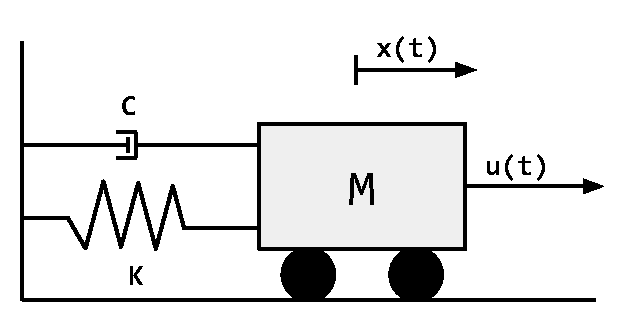
\includegraphics[width=0.44\textwidth]{chapter1/massSpringDamper}};
		\node [right of=img1,yshift=-0.8em](img2) {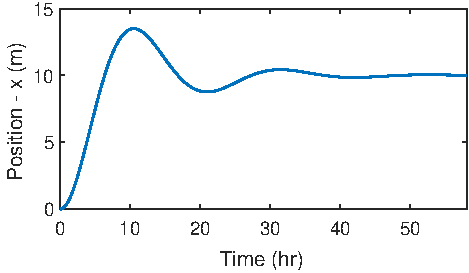
\includegraphics[width=0.47\textwidth]{chapter1/massSpringDamperPlot}};
	\end{tikzpicture}
	\caption{The schematic of a simple Mass-Spring-Damper system and its dynamical response to being forced by an unitary constant force.}
	\label{fig:intro01}
\end{figure}

In this simulation, quantities as the rise time, peak time, overshoot ratio and steady-state value of the visualized signal are examples of response specifications that can be defined to describe the system behavior to an external stimuli (in this case, a constant force of unit magnitude). These specified parameters are characteristic to responses of a class of systems known as \textit{underdamped second-order systems}, that will be discussed further in the document. 

A controller is used to calculate, for a time $t \in \left[ t_0, t_N \right]$, the necessary input $u(t)$ to produce an output $y(t)$ as close as possible to a desired reference signal $r(t)$. There are two common configurations, shown in Fig. \ref{fig:intro02}, of how to connect the controller to the system.

\begin{figure}[ht] 
	\begin{subfigure}{0.65\textwidth}
	\vskip0.25cm
	\begin{tikzpicture}[auto, node distance=2.5cm,>=latex']
	    % We start by placing the blocks
	    \node [input, name=input] {};
	    \node [block, minimum width=6em, minimum height=3.5em, right of=input] (controller) {\textbf{Controller}};
	    \node [block, minimum width=6em, minimum height=3.5em, right of=controller,
	            node distance=3.5cm] (system) {\textbf{System}};
	    % We draw an edge between the controller and system block to 
	    % calculate the coordinate u. We need it to place the measurement block. 
	    \draw [->, thick] (controller) -- node[pos=0.5] {$u(t)$} node[name=u] {} (system);
	    \node [output, right of=system, node distance=3cm] (output) {};
	
	    % Once the nodes are placed, connecting them is easy. 
	    \draw [draw,->, thick] (input) -- node[pos=0.1] {$r(t)$}  (controller);
	    \draw [->, thick] (system) -- node [name=y,pos=0.4]{} node[pos=0.75]{$y(t)$} (output);
	\end{tikzpicture}
	
	\end{subfigure} \\ \vspace{.6ex}
	\hfill \begin{subfigure}{0.65\textwidth}
	\vskip0.75cm
	\begin{tikzpicture}[auto, node distance=2.5cm,>=latex']
	    % We start by placing the blocks
	    \node [input, name=input] {};
	    \node [sum, right of=input] (sum) {};
	    \node [block, minimum width=6em, minimum height=3.5em, right of=sum] (controller) {\textbf{Controller}};
	    \node [block, minimum width=6em, minimum height=3.5em, right of=controller,
	            node distance=3.5cm] (system) {\textbf{System}};
	    % We draw an edge between the controller and system block to 
	    % calculate the coordinate u. We need it to place the measurement block. 
	    \draw [->, thick] (controller) -- node[pos=0.5,name=u] {$u(t)$} (system);
	    \node [output, right of=system, node distance=3cm] (output) {};
	    \node [block, minimum width=6em, minimum height=3.5em, below of=u] (measurements) {\textbf{Sensor}};
	
	    % Once the nodes are placed, connecting them is easy. 
	    \draw [draw,->, thick] (input) -- node[pos=0.1] {$r(t)$} node[pos=0.8] {$+$}  (sum);
	    \draw [->, thick] (sum) -- node[pos=0.4] {$e(t)$} (controller);
	    \draw [->, thick] (system) -- node [name=y,pos=0.4]{} node[pos=0.75]{$y(t)$} (output);
	    \draw [->, thick] (y) |- (measurements);
	    \draw [->, thick] (measurements) -| node[pos=0.95] {$-$} node [near end] {} (sum);
	\end{tikzpicture}
	\end{subfigure}
	
	\caption{The two most popular configurations for connecting controllers to dynamical systems. }
	\label{fig:intro02}
\end{figure}

The configuration shown in the upper left of Fig. \ref{fig:intro02}, known as the \textit{Open-Loop Controller}, calculates the action as a function $u(t) = \pi(r, t)$, given an initial condition $y(t_0) = y_0$. In this case, the controller does not observe the output $y(t)$, and relies on the model to guarantee that the system is driven to the reference. Of course, if there are any external disturbances acting on this configuration, or if the model is not reliable enough, it is not possible to guarantee that the requirements are met. Thus, these type of controllers are not suitable for critical applications, and its use is restricted to systems where deviance from the desired reference can be tolerated. \textbf{[reference]}

In contrast, the configuration in the lower right of Fig. \ref{fig:intro02}, known as the \textit{Closed-Loop Controller} or \textit{Feedback Controller}, calculates the action as a function $u(t) = \pi(e, t)$, where $e(t) = r(t) - y(t)$ is the error between the reference and the actual response. Now, the controller will observe the system output, trough some sensor device, and compares it to the desired reference in order to calculate a \textit{corrective action}. This feedback property can make the system reject disturbances while still driving it to the desired reference. Thus, the Feedback Controller became the most popular choice of controller configuration in industry for a wide range of applications, even for critical ones.  \textbf{[reference]}

\section{Chemical reactor Systems}

A chemical reaction, the transformation of a chemical substance into another, is a process central to chemistry and to nature itself. A reaction equation is an intuitive representation of such transformations. For instance, consider the following equation representing a \textit{synthesis} reaction:
\begin{equation}
    A + 2 B \longrightarrow 3 C + D 
.\end{equation} 

\noindent In this equation, the compounds $A$ and $2 B$ forms the set of reactants, $\mathcal{R}$, while $3 C$ and $D$ forms the set of products, $\mathcal{P}$. The coefficients in such equations are the stoichiometric numbers, providing an information about proportionality between the quantity of each substances in this reaction. 

Usually the products can be directly used as reactants in another reaction, in which case they can also be referred as an intermediate product (or byproduct), and the equations can be appended in a ``series" representation. In this case, each $k$-th intermediate product forms a set $\mathcal{I}_k$. In addition to a chain of series reactions, there is also the possibility of different reactions to occur in parallel, in the same system. The combination of these sets of reactants, byproducts, products and reactions are often referred as a \textit{chemical reaction network}, and the associated equation can be represented in general form as:
\begin{equation} \label{eq:chemNetwork}
\left\{ \begin{matrix}
    \mathbb{R}^{(1)}  & \longrightarrow & \mathcal{I}^{(1)}_1  &  \longrightarrow & \cdots & \longrightarrow & \mathcal{I}^{(1)}_{M_1} & \longrightarrow & \mathcal{P}^{(1)} \\
    \mathbb{R}^{(2)} & \longrightarrow & \mathcal{I}^{(2)}_1  &  \longrightarrow & \cdots & \longrightarrow & \mathcal{I}^{(2)}_{M_2} & \longrightarrow & \mathcal{P}^{(2)} \\
    \vdots &  & \vdots &  & \vdots &  & \vdots &  & \vdots \\
    \mathbb{R}^{(N)} & \longrightarrow & \mathcal{I}^{(N)}_1  &  \longrightarrow & \cdots & \longrightarrow & \mathcal{I}^{(N)}_{M_N} & \longrightarrow & \mathcal{P}^{(N)} \\
\end{matrix} \right.
.\end{equation} 

Moreover, chemical reactions displays a dynamical behavior concerning the speed at which a reaction occurs. This rate of reaction, its \textit{kinetics}, are dependent on the conditions in the environment, such as temperature and pressure, and on some properties of the reaction itself. In the case of a \textit{isothermal process}, i.e., when the temperature in the environment remains constant, this rate can be calculated as a constant $K$, leading to a representation on the form:
\begin{equation}
    \mathcal{R} \overset{K}{\longrightarrow} \mathcal{P}
.\end{equation} 

When the temperature in the environment is not constant, the process is said to be endothermic or exothermic if, respectively, it consumes or produces energy. The kinetics of the reactions in such processes are usually functions of the temperature $T$ which are assumed to follow the following form, known as the Arrhenius equation
\begin{equation} \label{eq:arrhenius1}
    K(T) = K_0 e^{\frac{-E/R}{T}}
,\end{equation}

\noindent where $K_0$ is the nominal kinetic rate, $E$ is an activation energy associated with the reaction, $R$ is the universal gas constant and $T$ is the absolute temperature (in kelvins).

In practice, these chemical reactions are produced by mixing the reactants in some environment with adequate conditions. In order to control the quantities of these substances, actual processes consists in a manipulation of the concentrations of reactants in some container, usually by providing a mass flow of these substances through some fluid. A major interest is to manipulate the reactants in some way to produce a desired concentration of one or more products in the chemical reaction network, allowing this problem to be addressed by a control engineering perspective. A \textit{chemical reactor system}, depicted in Fig. Fig. \ref{fig:intro03a}, is a system where the concentration of some reactants is manipulated to produce a desired concentration of some products, given a chemical reaction network describing the reaction between these entities.

\begin{figure} \centering
	\begin{subfigure}{0.47\textwidth}
	\resizebox{\textwidth}{!}{
	\begin{tikzpicture}[auto, node distance=3cm, >=latex']
		\node [input] (input1) {};
		\node [block, right of=input1, minimum width=8em, minimum height=5em] (system) {{\large \bfseries System}};
		\node [output, right of=system] (output) {};
		
		\node [below of=system, node distance=6em] {$\left\{ \begin{matrix} \mathbb{R}^{(1)}  & \overset{K_{11}}{\longrightarrow} & \cdots & \overset{K_{1n}}{\longrightarrow} &  \mathcal{P}^{(1)} \\ \vdots &  & \vdots &  & \vdots \\ \mathbb{R}^{(N)} &  \overset{K_{n1}}{\longrightarrow} & \cdots & \overset{K_{nn}}{\longrightarrow} & \mathcal{P}^{(N)} \\\end{matrix} \right.$};		
		
		\draw[->, line width=0.5mm] (input1) node[pos=0.1]{Reactants} -- (system);
		\draw[->, line width=0.5mm] (system) -- node[pos=0.9]{Products} (output);
	\end{tikzpicture}}
	
	\caption{Isothermal chemical reactor}
	\label{fig:intro03a}
	\end{subfigure} \hfill
	\begin{subfigure}{0.49\textwidth}
	\resizebox{\textwidth}{!}{
	\begin{tikzpicture}[auto, node distance=3cm, >=latex']
		\node [input] (input1) {};
		\node [input, below of=input1, node distance=1.5em] (input2) {};
		\node [input, below of=input2, node distance=1.5em] (input3) {};
		\node [block, right of=input2, minimum width=8em, minimum height=5em] (system) {{\large \bfseries System}};
		\node [output, right of=system] (output2) {};
		\node [output, above of=output2, node distance=1.5em] (output1) {};		
		\node [output, below of=output2, node distance=1.5em] (output3) {};
		
		\node [below of=system, node distance=6em] {$\left\{ \begin{matrix} \mathbb{R}^{(1)}  & \overset{K_{11}(T)}{\longrightarrow} & \cdots & \overset{K_{1n}(T)}{\longrightarrow} &  \mathcal{P}^{(1)} & & \Delta H_1 \\ \vdots &  & \vdots &  & \vdots  & &  \\ \mathbb{R}^{(N)} &  \overset{K_{n1}(T)}{\longrightarrow} & \cdots & \overset{K_{nn}(T)}{\longrightarrow} & \mathcal{P}^{(N)}  & & \Delta H_n \\ \end{matrix} \right.$};				
		
		\draw[->, line width=0.5mm] (input1) node[pos=0.1]{Reactants} -- (input1-|system.west);
		\draw[->, line width=0.5mm] (input3) -- node[pos=0.1]{Heat Capacity} (input3-|system.west);
		\draw[<-, line width=0.5mm] (output1) -- node[pos=0.1,yshift=1.5em]{Products} (output1-|system.east);
		\draw[<-, line width=0.5mm] (output3) -- node[pos=0.1,yshift=1.5em]{Temperature} (output3-|system.east);
	\end{tikzpicture}}
	
	\caption{Non-isothermal chemical reactor}
	\label{fig:intro03b}
	\end{subfigure}	
	
	\caption{General graphical representations of common chemical reactor systems.}
	\label{fig:intro03}
\end{figure}

When the process is non-isothermal, the occurrence of a reaction contributes to the entropy of the environment, and consequently affects the kinetics of the subsequent ones. To compensate for this, practical applications also try to control the conditions in the environment using instruments external to the reactions themselves. Because of the use of the Arrhenius equation to model these reaction rates, this control is usually implemented through a cooling or heating system coupled to the original reactor system, resulting in the schematic on Fig. \ref{fig:intro03b}. Moreover, note that the equation associated with non-isothermal reactions suffers a change of notation to include the value of entropy change, denoted $\Delta H$, resulting in the following general equation known as the \textit{reaction heat equation}:
\begin{equation}
\begin{matrix}    
	\mathcal{R} \overset{K(T)}{\longrightarrow} \mathcal{P} & & \Delta H
\end{matrix}
.\end{equation} 

\section{Motivation}

The use of automatic controllers to impose a desired behaviour to physical systems is a practice ubiquitous in many engineering fields. In the last years, the price of digital computers have been dropping while their performance have been growing. Consequently, digital controllers have became the central key in developments in important and innovative fields such as aeronautics \textbf{[reference]}, autonomous driving \textbf{[reference]} and several industrial applications \textbf{[reference]}. In parallel, this theory is also useful to understand and bring inspiration from nature itself since, for instance, the mechanisms for temperature regulation observed in vertebrate animals behave as a feedback controller \cite{Heller:1978}.

Most recent developments in Control Theory focus on using Feedback Controllers to achieve \textit{Robust and Optimal Control} \textbf{[reference]}. This theory accounts for the design of controllers that deals with uncertainty, either from the model or from the observation of the system, and are able to achieve the control objectives in a \textit{optimal manner}. Despite being a few decades old, these fields have gained a lot of interest in the last years thanks to recent results in \textit{Machine Learning} theory, particularly in \textit{Reinforcement Learning}, which have been successful in applying optimization techniques for controlling artificial agents in environments loaded with uncertainty \textbf{[reference]}.

Furthermore, the specific application of controlling chemical reactor systems brings benefits from the fact that this class of dynamical system are present in most biological and industrial processes \textbf{[reference]}. In general, controllers can be used to guarantee safety constraints, maximize productivity and minimize the use of resources, in such a way that could not be achieved without automatic and high performing machinery. The inherent complexity and uncertainty existent in these systems also poses this control problem as a challenging research field still open to be explored.

\section{Objectives}

This works aims to provide a self-contained discussion of modeling and control of chemical rector systems in the perspective of modern control, with focus on optimal control theory. Therefore, the results are focused on \textit{state-feedback controllers} modeled in continuous time. Several properties of the dynamical models of such systems, both in the open-loop and feedback regime, are summarized in the document and the intention is to have a generalized mathematical framework to understand, evaluate and design those control systems. Finally, a specific problem concerning the control of a non-isothermal continuous reactor is explored to demonstrate an application of the theory developed throughout the document.

\section{Chapters Organization}

The chapters of this document are mainly organized in two parts. The first part, comprised by the chapters 2, 3 and 4, builds the necessary theoretical background and provides the mathematical framework for modeling and control of the discussed systems. The second part, comprised by the chapters 5 and 6, describes the experiments and results of applying these methods in real-world applications.

Individually, the chapters are organized as follows. Chapter 2 introduces the concept of dynamical models and their several properties with respect to a real system behavior. Chapter 3 discusses general results of state-feedback controllers and state observers. Chapter 4 presents the theory of optimal estimation and optimal control, in a broad perspective. Chapter 5 describes practical experiments in respect to a real-world continuous reactor system. Chapter 6 summarizes and discusses the results of these experiments, emphasizing the theory from the previous sections. Finally, chapter 7 concludes the document and highlight the most important results.


% %%%%%%%%%%%%%%%%%%%%%%%%%%%%%%%%%%%%%%%%%%%%%%%%%%%%%%%%%%%%%%%
% %%%%%%%%%%%%%%%%%%%%%%%%%%%%%%%%%%%%%%%%%%%%%%%%%%%%%%%%%%%%%%%
% 2 - Dynamical System Modelling
% ---------------------------------------------------------------
\clearpage
\chapter{Dynamical System Analysis}

This chapter discusses the mathematical models for dynamical systems. The sections starts by introducing a procedure to build models from physical principles and presenting equivalent common representations. Next, the time evolution of dynamical systems is analyzed in relation to the mathematical structure of such models. Finally, some important properties of the systems are defined and discussed. A discussion of the system evolution in the frequency domain is also presented.

\section{First Principles Models}

A dynamical system is a physical system whose state evolves with time. One can represent a dynamical system using the \textit{first principles} from physics, and formulate the evolution in time by calculating the rate of change of its state in respect to time. Thus, dynamical models are represented using differential equations with time derivatives. 

A straightforward procedure to model a system consists of identifying the variables of interest and relate them using conservation laws, such as conservation of mass, conservation of energy or conservation of momentum. The resulting models are in the form:
\begin{equation} \label{eq:massCons01}
    \begin{pmatrix}
        \text{Rate of} \\ \text{accumulation of} \\ \text{Mass/Energy/Momentum}  
    \end{pmatrix} = \begin{pmatrix}
        \text{Mass/Energy/Momentum} \\ \text{entering} \\ \text{the system}
    \end{pmatrix} - \begin{pmatrix}
        \text{Mass/Energy/Momentum} \\ \text{leaving} \\ \text{the system}
    \end{pmatrix}
.\end{equation}

The choice of which conservation law to use depends on the system itself. Usually, conservation of mass is used to relate dynamics of concentrations and volumes, or other material variables, while conservation of momentum is used to relate dynamics of motion. Since energy can be converted on form, the conservation laws of this quantity can be used to model several dynamics, such as the rate of change in heat, electrical charges or velocity of a system.

In the case of a chemical reactor system, the variables of interest are the concentrations of the chemical substances in the system. Hence, the rate of accumulation of a substance can be represented using the mass conservation law, or mass balance:
\begin{equation} \label{eq:massCons02}
\begin{split}
    \begin{pmatrix}
        \text{Accumulation} \\ \text{of mass} \\ \text{in the system}
    \end{pmatrix} &= 
    \begin{pmatrix}
        \text{Mass} \\ \text{entering} \\ \text{the system}
    \end{pmatrix} - \begin{pmatrix}
        \text{Mass} \\ \text{leaving} \\ \text{the system}
    \end{pmatrix} \\
    &= \left[ \begin{pmatrix}
        \text{Mass flow} \\ \text{entering} \\ \text{system}
    \end{pmatrix} + \begin{pmatrix}
        \text{Mass} \\  \text{produced} \\ \text{by reactions}
    \end{pmatrix} \right] - \left[ \begin{pmatrix}
        \text{Mass flow} \\ \text{leaving} \\ \text{system}
    \end{pmatrix} + \begin{pmatrix}
        \text{Mass} \\ \text{consumed} \\ \text{by reactions}
    \end{pmatrix} \right]
\end{split}
.\end{equation}

\begin{boxed-example}{(\textit{Mass Balance of Reactors})} \label{ex:isoReactSys01}
    For the sake of illustration, consider the process of obtaining a first principles model for the concentration of a general substance in a reactor system, as follows. Consider a system such as the one depicted in \ref{fig:intro03a}. First of all, one has to evaluate the mass flow through the system, as denoted in \eqref{eq:massCons02}. The mass of any substance $A$ entering and leaving the system, denoted respectively by $M_{in}$ and $M_{out}$, are assumed to be provided by a flow of fluid carrying the substance. Given a fluid inflow $F_{in}$, with density $\rho^{(A)}_{in}$, and an outflow $F_{out}$, with density $\rho^{(A)}_{out}$, the mass flow is calculated by equations:
    \begin{equation}
        \begin{matrix}
            M_{in} = \rho^{(A)}_{in} F_{in} &; & M_{out} = \rho^{(A)}_{out} F_{out}
        \end{matrix}
    .\end{equation}
    
    Now, one has to consider the quantities of mass that are consumed and produced by the reactions of the chemical reaction network associated to the system. In this case, consider the following reaction between two chemical compounds $X$ and $Y$, with stoichiometric numbers $\alpha$ and $\beta$:
    \begin{equation} \label{eq:simpleEq01}
        \alpha X \overset{K_{XY}}{\longrightarrow} \beta Y
    .\end{equation}
    
    Under the assumption that the reactant is in a dilute solution, the rate of this equation obeys the \textit{law of mass action} \cite{Horn:1972}. Given a constant kinetic rate $K_{XY}$ and the volume of the solution as $V$, the mass of $X$ consumed, $M^{(X)}_\text{cons}$, and the mass of $Y$ produced, $M^{(Y)}_\text{prod}$, are given by the power-laws:
    \begin{equation}
        \begin{matrix}
            M^{(X)}_\text{cons} = \cfrac{V}{\beta} K_{XY} (\rho_X)^{\alpha} &; & M^{(Y)}_\text{prod} = \cfrac{V}{\alpha} K_{XY} (\rho_X)^{\alpha}
        \end{matrix}
    ,\end{equation}
    
    \noindent where $\rho_X$ and $\rho_Y$ are the respective densities of these compounds. Assuming that the network represents a set of reactions occurring within an chemical solution of volume $V$, the mass of a substance $A$ that is consumed and produced by the reactions, named respectively $M_\text{cons}$ and $M_\text{prod}$, are given by summing over the contribution of each reaction on the network where $A$ is either a reactant or a product to any other compound $X$:
    \begin{equation}
    \begin{matrix}
            M_\text{cons} = V \displaystyle\sum_{\alpha A \rightarrow \beta X} \cfrac{1}{\beta} K_{AX} (\rho_A)^{\alpha} &; &  M_\text{prod} = V \displaystyle\sum_{\alpha X \rightarrow \beta A} \cfrac{1}{\beta} K_{XA} (\rho_X)^{\alpha}
    \end{matrix}
    .\end{equation}
    
    Finally, directly substituting these values in \eqref{eq:massCons02}, the mass balance of any substance $A$ in an isothermal chemical reactor system can be represented by the general dynamical model:
    \begin{equation}
    \begin{split}
        \begin{pmatrix}
        \text{Accumulation} \\ \text{of mass} \\ \text{in the system}
    \end{pmatrix} &= \left[ \begin{pmatrix}
        \text{Mass flow} \\ \text{entering} \\ \text{System}
    \end{pmatrix} + \begin{pmatrix}
        \text{Mass} \\  \text{produced} \\ \text{by reactions}
    \end{pmatrix} \right] - \left[ \begin{pmatrix}
        \text{Mass flow} \\ \text{leaving} \\ \text{System}
    \end{pmatrix} + \begin{pmatrix}
        \text{Mass} \\ \text{consumed} \\ \text{by reactions}
    \end{pmatrix} \right] \\
        \cfrac{d (\rho_A V)}{dt} &= \left[ \rho^{(A)}_{in} F_{in} + V \sum_{\alpha X \rightarrow \beta A} \cfrac{1}{\beta} K_{XA} (\rho_X)^{\alpha} \right] - \left[ \rho^{(A)}_{out} F_{out} + V \sum_{\alpha A \rightarrow \beta X} \cfrac{1}{\beta} K_{AX} (\rho_A)^{\alpha} \right]
    \end{split}
    .\end{equation}
    
    Since the system is closed, i.e., there are no leaks or unknown sources of fluids, the assumptions of a constant volume implies that $F_{in} = F_{out} = F$. Normalizing each term by the volume and substituting a new variable $q = F/V$ results in:
    \begin{equation} \label{eq:isoModel3}
            \cfrac{d (\rho_A)}{dt} = q (\rho^{(A)}_{in} - \rho^{(A)}_{out}) + \left( \sum_{\alpha X \rightarrow \beta A} \cfrac{1}{\beta} K_{XA} (\rho_X)^{\alpha} \right) - \left(\sum_{\alpha A \rightarrow \beta X} \cfrac{1}{\beta} K_{AX} (\rho_A)^{\alpha} \right)
    .\end{equation}
\end{boxed-example}

Notice some important restrictions to the use of the model just presented. First of all, to calculate the mass contribution of an individual reaction was necessary to use a model which assumes that the reactor system is actually comprised of a dilute solution in some closed container. In industry, this means that the reactor system is actually a tank containing the solution. The inflow and outflow of fluid can be represented by flows through pipes which can be manipulated by some valve or pump. An illustration of such physical system is exhibited at Fig. \ref{fig:tank01a}.

Furthermore, this model accounts for a single substance $A$, but the system is actually a solution of several compounds, each one with a specific concentration. From the model presented, it is visible that it is necessary to compute each concentration $\rho_X$ before actually computing the rate of change in $\rho_A$. However, from the same model, the computation of the rate of change of any $\rho_X$ may depend on $\rho_A$ itself. Therefore, the change of concentration inside the whole system is actually the result of a system of differential equations:
\begin{align}   \label{eq:isoSys01}
\begin{cases}
    \hfill \cfrac{d (\rho_{X_1})}{dt} &= f(\rho_{X_1}, \rho_{X_2}, ..., \rho_{X_n}, \rho_{in}^{(X_1)}, \rho_{out}^{(X_1)}, t) \\
    \hfill \cfrac{d (\rho_{X_2})}{dt} &= f(\rho_{X_1}, \rho_{X_2}, ..., \rho_{X_n}, \rho_{in}^{(X_2)}, \rho_{out}^{(X_2)}, t) \\
    & \vdots   \\
    \hfill \cfrac{d (\rho_{X_n})}{dt} &= f(\rho_{X_1}, \rho_{X_2}, ..., \rho_{X_n}, \rho_{in}^{(X_n)}, \rho_{out}^{(X_n)}, t)
\end{cases}
,\end{align}

\noindent where $X_1, X_2, ..., X_n$ are the chemical compounds inside the reactor and $f(\cdot)$ is the dynamical model presented in Example \ref{ex:isoReactSys01}.

\begin{figure}[ht] 
    \centering
    \begin{subfigure}{0.49\textwidth}   
        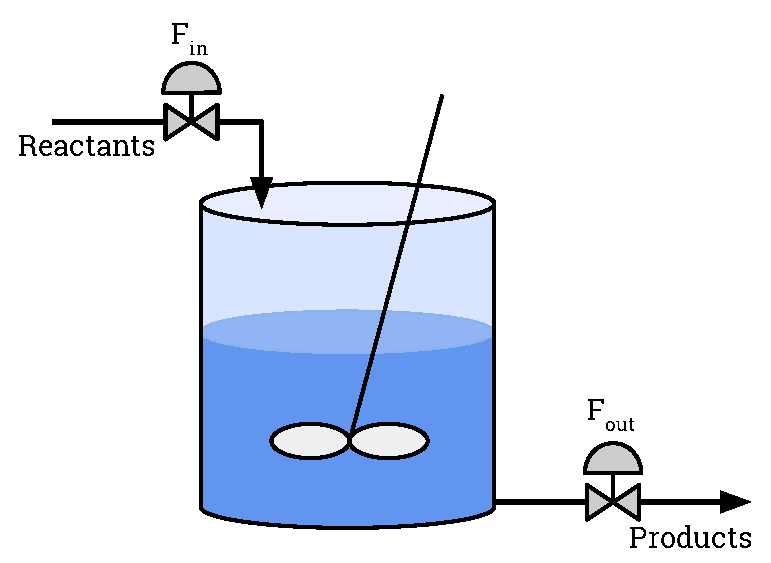
\includegraphics[width=\textwidth]{chapter2/tank01}
        \caption{$\ \ \ \ \ $}  \label{fig:tank01a}
    \end{subfigure}
    \begin{subfigure}{0.49\textwidth}   
        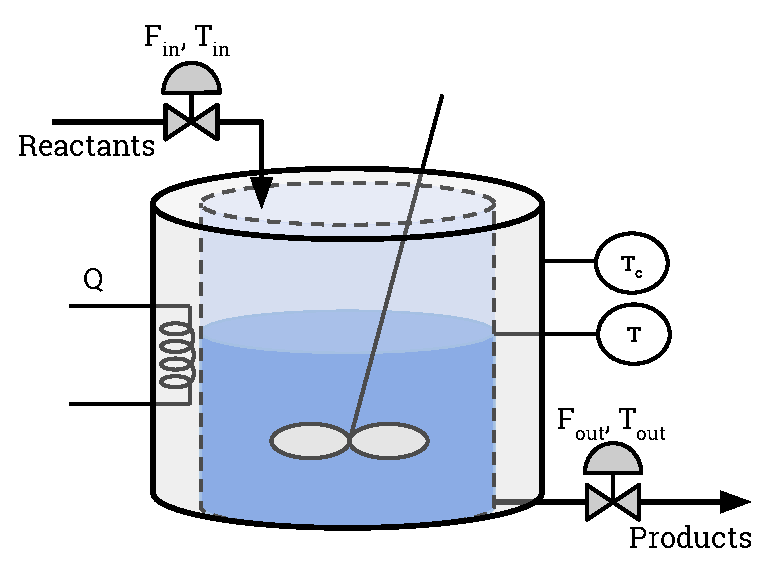
\includegraphics[width=\textwidth]{chapter2/tank02}
        \caption{$\ \ \ \ \ $} \label{fig:tank01b}
    \end{subfigure}
    
    \caption{Schematic representations of industrial reactor tanks for (a) a simple isothermal process and (b) a non-isothermal process with heating/cooling system.} 
    \label{fig:tank01}
\end{figure}

The model discussed so far is fairly simple. To account for more complex systems, the same modeling procedure can still be applied. For instance, it is possible to extend the description to account for exothermic and endothermic processes, when the temperature inside the system has a dynamical evolution and the dynamics of the reactions starts to depend on it.

When discussing non-isothermal processes, it is also common to discuss heating or cooling systems that tries to impose certain operational conditions to the reactions, as illustrated in Fig. \ref{fig:tank01b}. In exothermic processes, for instance, the heat accumulated in the system tends to grows as the reactions occurs, which can be very dangerous. One approach to regulate the temperature consists in involving the chemical solution, or the container containing it, with a material whose temperature can be manipulated, transferring or absorbing heat by conductance. The temperature of this material can be manipulated by, for instance, running a heated fluid or converting electrical energy to heat energy.

\begin{boxed-example}{(Non-isothermal Reactor System)} \label{ex:exoReactSys01}
    Consider the process of obtaining a first principle model for a non-isothermal reactor, such as the one depicted in \ref{fig:intro03b}. In this case, the kinetic rates will follow the Arrhenius equation from \eqref{eq:arrhenius1}. Following the same procedure from Example \ref{ex:isoReactSys01}, a dynamical model for the concentrations of a substance $A$, inside this reactor, can be formulated as: 
    \begin{equation} \label{eq:exoModel1}
            \cfrac{d (\rho_A)}{dt} = q (\rho^{(A)}_{in} - \rho^{(A)}_{out}) + \left( \sum_{\alpha X \rightarrow \beta A} \cfrac{1}{\beta} K_{XA} e^{-\frac{E_{XA}/R}{T}} (\rho_X)^{\alpha} \right) - \left(\sum_{\alpha A \rightarrow \beta X} \cfrac{1}{\beta} K_{AX} e^{-\frac{E_{AX}/R}{T}} (\rho_A)^{\alpha} \right)
    ,\end{equation}

    \noindent where $E_{XA}$ and $E_{AX}$ are the activation energy needed for each reaction, and the rest of the parameters are still the same as defined in Example \ref{ex:isoReactSys01}.  
    
    Furthermore, since the process is non-isothermal, the reactions will cause a change of temperature inside the reactor system. Consider the temperature inside the reactor, denoted as $T$. In this case, it is possible to relate its dynamics to the conservation law:  
    \begin{equation}
    \begin{split}
        \begin{pmatrix}
            \text{Accumulation} \\ \text{of thermal energy} \\ \text{in the system}
        \end{pmatrix} &= \begin{pmatrix}
            \text{Thermal energy} \\ \text{entering} \\ \text{the system}
        \end{pmatrix} - \begin{pmatrix}
            \text{Thermal energy} \\ \text{leaving} \\ \text{the system}
        \end{pmatrix} \\
         &= \begin{pmatrix}
            \text{Heat flow} \\ \text{entering} \\ \text{the system}
        \end{pmatrix} - \begin{pmatrix}
            \text{Heat flow} \\ \text{leaving} \\ \text{the system}
        \end{pmatrix} + \begin{pmatrix}
            \text{Entropy} \\ \text{contribution} \\ \text{from reactions}
        \end{pmatrix}
    \end{split}
    .\end{equation}
    
    It is well known, from Fourier's law \textbf{[seek reference]}, that the transfer of heat by conduction between the reactor and the coolant/heater, in their respective contact interfaces, is proportional to $(T_C - T)$, where $T_C$ represents the temperature of the latter. Moreover, another identifiable source of heat transfer consists in the fluid flow entering and leaving the system. Similarly for the conduction, this heat contribution should also be proportional to $(T_{in} - T_{out})$, where $T_{in}$ and $T_{out}$ are respectively the temperature of the fluid entering and leaving the reactor.
    
    The entropy contribution from a reaction $\alpha X \rightarrow \beta Y$, denoted as $S_{XY}$, is proportional to the concentration of $\rho_X$ consumed, or produced, by the reactions multiplied by the energy that it liberates or absorbs \textbf{[reference]}:
    \begin{equation}
        S_{XY} \sim K_{XY} e^{-\frac{E_{XY}}{T}} (\rho_X)^{\alpha} \Delta H_{XY}
    .\end{equation}

    All the proportionality can be turned into equalities by imposing real constant factors that are calculated independent of the dynamical variables. In the case of the heat transfer from the fluid, this constant factor is the flow-rate $q$ itself. Plugging all together, and summing the entropy contribution from each reaction, the accumulation of heat can be modeled:
    \begin{equation}
        \cfrac{d(T)}{dt} = q(T_{in} - T_{out}) + \eta (T_C - T) + \delta \sum_{\alpha A \rightarrow \beta X} K_{AX} e^{-\frac{E_{AX}}{T}} (\rho_A)^{\alpha} \Delta H_{AX}
    .\end{equation}
    
    Consider now the heating/cooling system involving the reactor system. From the choice of design of this apparatus, it is possible to manipulate the temperature of its material using a heat capacity $Q$, up to a real factor of $\gamma$. Similar to the temperature inside the container, there is the conduction of heat between the healing/cooling system and the walls of the container for the reactor. Therefore, the model of heat accumulation for this quantity is simply given by:
    \begin{equation}
        \cfrac{d(T_C)}{dt} = \gamma Q + \beta (T - T_C)
    .\end{equation}
\end{boxed-example}

The non-isothermal reactor system is a more general model that accounts for the fact that the temperature of the environment is usually not constant. From this assumption, the flow entering and leaving the system are also not assumed to have the same temperature that the fluid inside the reactor. In practical applications, the temperature of the fluid inflow can either be manipulated or measured, where the temperature of the fluid outflow is actually assumed to be equal to the temperature inside the reactor. In addition, the proportionality constants are not functions of any dynamical variable, so they can be calculated before the operation of the system by using the properties of the materials and containers.

In the case of this model, the rate of changes in the chemical concentrations depends on the temperature through the Arrhenius equation. However, the temperature of the reactor itself depends on those concentrations. So, as noted in \eqref{eq:isoSys01}, the dynamical model of the entire reactor is a system of differential equations relating all those quantities.


\section{Canonical Representations for Dynamical Models}

The last section presented the foundation for modeling a dynamical system using first principles from physics. Although it is a well-defined formulation, the resulting models are not guaranteed to be practical in a mathematical sense. This motivates a discussion about possible canonical formats for such models, which would allow for systematic analysis approaches. In the perspective of control theory, that are two main formats for the model of a system: the \textit{Input-Output} (IO) and the \textit{State-Space} (SS) representations.

An input-output representation is a simple model that describes the entire system using only two types of variables, and their derivatives. Therefore, the dimension of these variables and the order of derivatives at each differential equation provides the information about the structure of the model. For instance, in the case where $p = r = 1$ the system can be classified as a \textit{Single-Input Single-Output} (SISO) configuration, whereas it is classified as a \textit{Multiple-Input Multiple-Output} (MIMO) configuration if $p,r > 1$. A formal definition is given below.

\begin{boxed-definition}{(Input-Output Representation)} \label{def:IORepr01}
    An Input-Output (IO) representation of a dynamical system with $p \geq 1$ output variables, represented by $\bm{y} : \mathbb{R} \rightarrow \mathbb{R}^{p}$, and $r \geq 1$ input variables, represented by $\bm{u} : \mathbb{R} \rightarrow \mathbb{R}^{r}$, is the system of differential equations:
    \begin{equation} \label{eq:IERepr01}
    \begin{cases}
        h_1 \left( y_1, \dot{y_1}, ..., y_1^{(n_1)}, u_1, \dot{u}_1, ..., u^{(m_{11})}_1, u_2, \dot{u}_2, ..., u^{(m_{12})}_2, ..., u_r, \dot{u}_r, ..., u^{(m_{1r})}_r, t   \right) = 0 & \\
        h_2 \left( y_2, \dot{y_2}, ..., y_2^{(n_2)}, u_1, \dot{u}_1, ..., u^{(m_{21})}_1, u_2, \dot{u}_2, ..., u^{(m_{22})}_2, ..., u_r, \dot{u}_r, ..., u^{(m_{2r})}_r, t   \right) = 0 & \\
         \vdots \hfill & \\
        h_p \left( y_p, \dot{y_p}, ..., y_p^{(n_p)}, u_1, \dot{u}_1, ..., u^{(m_{p1})}_1, u_2, \dot{u}_2, ..., u^{(m_{p2})}_2, ..., u_r, \dot{u}_r, ..., u^{(m_{pr})}_r, t   \right) = 0 &
    \end{cases}
    ,\end{equation}
    
    \noindent where:
    \begin{equation*}
    \begin{matrix}
        \dot{y}(t) = \cfrac{d y(t)}{dt}, & \ddot{y}(t) = \cfrac{d^2 y(t)}{dt^2}, & \cdots, & y^{(n)}(t) = \cfrac{d^n y(t)}{dt^n}
    \end{matrix}
    \end{equation*}

	\noindent and    
    \begin{equation*}
    \begin{matrix}
        \dot{u}(t) = \cfrac{d u(t)}{dt}, & \ddot{u}(t) = \cfrac{d^2 u(t)}{dt^2}, & \cdots, & u^{(n)}(t) = \cfrac{d^n u(t)}{dt^n}
    \end{matrix}
    .\end{equation*}
\end{boxed-definition}

This model presents a cause-and-effect interpretation of the system where the direct relationship between the input and output signal, and its derivatives, are equated as if the system is a processing unit. In practice, the input signals $\bm{u}(t)$ are the manipulated variables of the system, where the output signals $\bm{y}(t)$ are the observations of the controlled variables. This representation brings an easy visualization on how a desired system behavior can be achieved by applying a specific input signal, posing as a practical framework for designing controllers. 

The State-Space representation is another formulation for a dynamical model, centered in the concept of \textit{state variables}. In a formal definition, the set of state variables is the smallest set of linearly independent variables that can unequivocally determine the value of all the states variables given an initial state $\bm{x}(t_0)$, at time $t_0 \in \mathbb{R}$, and a forcing function $\bm{u}(t)$, for any time $t \geq t_0$. From a physical perspective, however, these variables may account for quantities that can describe the dynamics of the system, such as position or velocities. In comparison to the Input-Output representation, this formulation poses a simpler mathematical model, since it is composed by a system of first order ordinary differential equations and a system of algebraic equations. However, this model presents a semantical improvement over the latter since the inclusion of the state variables expands the internal description of the system. A formal definition is given below.

\begin{boxed-definition}{(State-Space Representation)} \label{th:SSRepr01}
    A State-Space (SS) representation of a system with $n \geq 1$ states variables, represented by $\bm{x} : \mathbb{R} \rightarrow \mathbb{R}^{n}$, for $p \geq 1$ output variables, represented by $\bm{y} : \mathbb{R} \rightarrow \mathbb{R}^{p}$, and $r \geq 1$ input variables, represented by $\bm{u} : \mathbb{R} \rightarrow \mathbb{R}^{r}$, is given by the systems of state and output equations:
    \begin{align} \label{eq:SSRepr01}
    \begin{split}
    \textbf{State Equations:}\ \ \ \ \ \ \ \ \ \ \ \ \ \ \ \ \ \ \ \ \ \  \hfill & \textbf{ Output Equations:} \hfill \\
    \begin{cases}
        \dot{x}_1(t) = f_1(x_1, ..., x_n, u_1, ..., u_r, t) \\
        \dot{x}_2(t) = f_2(x_1, ..., x_n, u_1, ..., u_r, t) \\
        \vdots \\
        \dot{x}_n(t) = f_n(x_1, ..., x_n, u_1, ..., u_r, t)
    \end{cases} \hfill &;  \begin{cases}
        y_1(t) = g_1(x_1, ..., x_n, u_1, ..., u_r, t) \\
        y_2(t) = g_2(x_1, ..., x_n, u_1, ..., u_r, t) \\
        \vdots \\
        y_p(t) = g_p(x_1, ..., x_n, u_1, ..., u_r, t) \hfill
    \end{cases}
    \end{split}
    ,\end{align}
    
    \noindent or, in the matrix form:
    \begin{align} \label{eq:SSRepr02}
    \begin{cases}
        \dot{\bm{x}}(t) = \bm{f}(\bm{x}(t), \bm{u}(t), t) \\
        \bm{y}(t) = \bm{g}(\bm{x}(t), \bm{u}(t), t)
    \end{cases}
    .\end{align}
\end{boxed-definition}

\begin{figure}[ht] 
    \centering
    \begin{subfigure}{0.49\textwidth}
        \centering  
        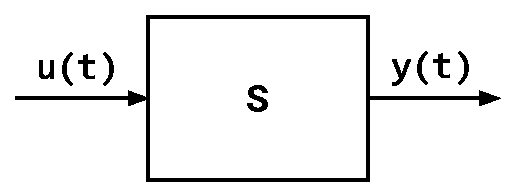
\includegraphics[scale=0.7]{chapter2/model01}
        \caption{}  \label{fig:model01a}
    \end{subfigure}
    \begin{subfigure}{0.49\textwidth}   
    \centering
        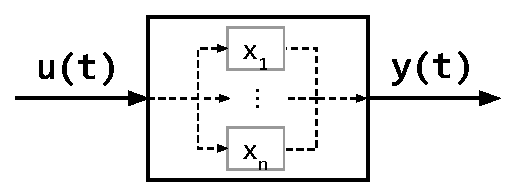
\includegraphics[scale=0.7]{chapter2/model02}
        \caption{} \label{fig:model01b}
    \end{subfigure}
    
    \caption{Graphical interpretation of (a) Input-Output models and (b) State-Spaces models.} 
    \label{fig:model1}
\end{figure}

A graphical illustration of both representations is shown at Fig. \ref{fig:model1}. In the light of these formulations, a system can be classified with respect to the model mathematical structure. There are five main properties used for this classification: whether the system is causal or non-causal, linear or nonlinear, dynamical or instantaneous, time-invariant or time-varying and with or without delay. The necessary and sufficient conditions for each one of these properties are summarized in Table \ref{table:classes01}.

\begin{table}[!ht]
    \centering
    \begin{tabular}{r | c | c }
     & \textbf{Input-Output} & \textbf{State-Space} \\
    \hline 
        \textbf{Causal}         & \makecell{$m_{ij} \leq n_k$\\$i \in [1,..., p],\ j \in [1,...,r]$} & Always causal \\
    \hline 
        \textbf{Linear}         & \makecell{$h_i(\cdot) = \sum_{j=0}^{n_i} y^{(j)} + ... \ \ \ \ \ \ \ \ $\\$ \ \ \ \ \ \ \ \ \ \ \ \ ... + \sum_{k=1}^{r} \sum_{l=0}^{m_{ik}} u_k^{(l)}$\\$i \in [1,2,...,p]$} & \makecell{$f_i = \bm{a}_i(t) \bm{x}(t) + \bm{b}_i(t) \bm{u}(t), i = 1,2,...,n$ \\ $g_j = \bm{c}_j(t) \bm{x}(t) + \bm{d}_j(t) \bm{u}(t), j = 1,2,...,p$ \\ $\bm{a}_i,\bm{c}_j \in \mathbb{R}^{1 \times n}$ and $\bm{b}_i, \bm{d}_j \in \mathbb{R}^{1 \times r}$} \\
    \hline 
        \textbf{Dynamical}      & \makecell{$n_i > 0$ or $m_{jk} > 0$\\$i, j \in [1,...,p],\ k \in [1,...,r]$} & $n > 0$ \\
    \hline 
        \textbf{Time-Invariant} & \makecell{$h_i(y_i(t),...,u_1(t),...,u_r(t)) = 0$\\$i \in  [1,2,...,p]$} & \makecell{$\dot{\bm{x}}(t) = \bm{f}(\bm{x}(t), \bm{u}(t))$ \\ $\bm{y}(t) = \bm{g}(\bm{x}(t), \bm{u}(t))$} \\
    \hline 
        \textbf{Without-Delay}  & \makecell{All the signals share\\the same time arguments} & \makecell{All the signals share\\the same time arguments} \\
    \end{tabular} 
    \caption{Necessary and sufficient conditions for different classes of models.}
    \label{table:classes01} 
\end{table} 

This work focus on dynamical linear systems, since its models are the most well studied in the control theory community. In reality, a physical system is always causal, nonlinear and time-varying \cite{Vidyasagar:2002}, but the models can be assumed differently with fairly accuracy. The benefit of linear systems is that it obeys the superposition principle, and a linear combination of the inputs directly causes the exact same linear combination of the individual outputs. Under the assumption of a linear system, a nice result is that the vectorial functions $\bm{f}(\cdot)$ and $\bm{g}(\cdot)$ of the State-Space representation in \eqref{eq:SSRepr03} reduces to simple matrix forms.

\begin{boxed-definition}{(Linear State-Space Representation)}
    A State-Space representation describing a linear system with state vector $\bm{x}(t) : \mathbb{R} \rightarrow \mathbb{R}^{n}$, output vector $\bm{y}(t) : \mathbb{R} \rightarrow \mathbb{R}^{p}$ and input vector $\bm{u}(t) : \mathbb{R} \rightarrow \mathbb{R}^{r}$ is given by the system of equations: 
    \begin{align} \label{eq:SSRepr04}
    \begin{cases}
        \dot{\bm{x}}(t) = \bm{A}(t) \bm{x}(t) + \bm{B}(t) \bm{u}(t) & \\
        \bm{y}(t) = \bm{C}(t) \bm{x}(t) + \bm{D}(t) \bm{u}(t) &
    \end{cases}
    ,\end{align}

    \noindent where $\bm{A}(t) : \mathbb{R} \rightarrow \mathbb{R}^{n \times n}$, $\bm{B}(t) : \mathbb{R} \rightarrow \mathbb{R}^{n \times r}$, $\bm{C}(t) : \mathbb{R} \rightarrow \mathbb{R}^{p \times n}$ and $\bm{D}(t) : \mathbb{R} \rightarrow \mathbb{R}^{p \times r}$. In the case of a time-invariant linear system, these matrices becomes constants. 
\end{boxed-definition}

This formulation has the advantage that the time response of the system can be easily calculated and that the analysis of the dynamics follows well-established results from linear algebra applied to the matrices $\bm{A}(t)$, $\bm{B}(t)$, $\bm{C}(t)$ or $\bm{D}(t)$, as well as for the vectors $\bm{x}(t)$ and $\bm{u}(t)$. Furthermore, the physical interpretation of the system through the state variables becomes straightforward in this model.

In addition to the State-Space representation, the linear assumption also benefits Input-Output representations. One major analytical tool that can be used in these cases is to transform this model to a frequency domain, using a linear transform operator, in order to simplify the solution for the differential equations. The most popular choice of transformation is the \textit{Laplace transform}, $\mathcal{L}\{ h(t) \}$, which converts functions in time to functions in complex frequencies. Using the properties of this operator, differential equations are converted to simple algebraic equations.

\begin{boxed-definition}{(Transfer Function)} \label{th:transFun01}
    Given a linear model for a SISO system, with initial conditions $\bm{y}(0^-) = \bm{u}(0^-) = \bm{0}$, in the Input-Output formulation:
    \begin{equation}
    \begin{split}
        \alpha_n \cfrac{d^n y(t)}{dt^n} + \cdots + \alpha_{1} \cfrac{d y(t)}{dt} + \alpha_{0} y(t) &= \beta_m \cfrac{d^m u(t)}{dt^m} + \cdots + \beta_{1} \cfrac{d u(t)}{dt} + \beta_{0} u(t)
    \end{split}
    ,\end{equation}
    
\noindent its correspondent transfer function, calculated in the Laplace domain, is defined as:
    \begin{equation} \label{eq:transFun01}
         G(s) = \cfrac{Y(s)}{U(s)} = \cfrac{\beta_m s^m + \beta_{m-1} s^{m-1} + \cdots + \beta_{1} s + \beta_0}{\alpha_n s^n + \alpha_{n-1} s^{n-1} + \cdots + \alpha_{1} s + \alpha_0}
    .\end{equation}
\end{boxed-definition}

An indirect result of this is that the SS representation can be converted to the IO representation using the Laplace transform operator, leading to a notion of equivalence between the two representations. Notice that the extension to the MIMO case is straightforward: just compute the transfer function between each pair of input and output, leading to the matrix $\bm{G} \in \mathbb{C}^{p \times r}$, for a system with $p$ outputs and $r$ inputs. For the general linear case, this matrix has the form:
\begin{align}
\bm{G}(s) = 
\begin{bmatrix}
	\cfrac{Y_1(s)}{U_1(s)} & \cfrac{Y_1(s)}{U_2(s)} & \cdots & \cfrac{Y_1(s)}{U_r(s)} \vspace{0.7ex} \\
	\cfrac{Y_2(s)}{U_1(s)} & \cfrac{Y_2(s)}{U_2(s)} & \cdots & \cfrac{Y_2(s)}{U_r(s)} \vspace{0.7ex} \\
	\vdots & \vdots & \ddots & \vdots \vspace{0.7ex} \\
	\cfrac{Y_p(s)}{U_1(s)} & \cfrac{Y_p(s)}{U_2(s)} & \cdots & \cfrac{Y_p(s)}{U_r(s)}
\end{bmatrix} =
\begin{bmatrix}
	\cfrac{\beta_{m_{11}}^{(11)} s^{m_{11}} + \cdots + \beta^{(11)}_{0}}{\alpha^{(1)}_{n_1} s^{n_1} + \cdots + \alpha^{(1)}_0} & \cdots & \cfrac{\beta_{m_1}^{(1r)} s^{m_{1r}} + \cdots + \beta^{(1r)}_0}{\alpha^{(1)}_{n_1} s^{n_1} + \cdots + \alpha^{(1)}_0} \vspace{0.7ex} \\
	\cfrac{\beta_{m_{21}}^{(21)} s^{m_{21}} + \cdots + \beta^{(21)}_{0}}{\alpha^{(2)}_{n_2} s^{n_2} + \cdots + \alpha^{(2)}_0} & \cdots & \cfrac{\beta_{m_2}^{(2r)} s^{m_{2r}} + \cdots + \beta^{(2r)}_0}{\alpha^{(2)}_{n_2} s^{n_2} + \cdots + \alpha^{(2)}_0} \vspace{0.7ex} \\
	\vdots & \ddots & \vdots \vspace{0.7ex} \\
	\cfrac{\beta_{m_{p1}}^{(p1)} s^{m_{p1}} + \cdots + \beta^{(p1)}_{0}}{\alpha^{(p)}_{n_p} s^{n_p} + \cdots + \alpha^{(p)}_0} & \cdots & \cfrac{\beta_{m_p}^{(pr)} s^{m_{pr}} + \cdots + \beta^{(pr)}_0}{\alpha^{(p)}_{n_p} s^{n_p} + \cdots + \alpha^{(p)}_0} 
\end{bmatrix}
.\end{align}

\begin{boxed-theorem}{(Passage from SS to IO)} \label{th:SSToIO}
    Consider a linear and time-invariant system in State-Space form with initial states $\bm{x}(0^-) = \bm{0}$ and represented as:
    \begin{align}
    \begin{cases}
        \dot{\bm{x}}(t) = \bm{A} \bm{x}(t) + \bm{B} \bm{u}(t) \\
        \bm{y}(t) = \bm{C} \bm{x}(t) + \bm{D} \bm{u}(t) \\
    \end{cases}     
    .\end{align}
    
\noindent The equivalent system in Input-Output representation is given by the transfer function:
    \begin{align}
    \bm{G}(s) = \bm{C} (s\bm{I} - \bm{A})^{-1} \bm{B} + \bm{D}
    .\end{align}
\end{boxed-theorem}
 
\begin{proof}
    Applying the Laplace formation to both sides of the equation, using the property of derivative in time, results in:
    \begin{equation} \label{eq:convertSSIO01}
    \begin{split}
        \mathcal{L} \left\{ \dot{\bm{x}}(t) \right\} &= \bm{A} \mathcal{L} \left\{ \bm{x}(t) \right\} + \bm{B} \mathcal{L} \left\{ \bm{u}(t) \right\} \\
        s \bm{X}(s) - \dot{\bm{x}}(0^-) &= \bm{A} \bm{X}(s) + \bm{B} \bm{U}(s) \\
    \end{split}
    .\end{equation}

\noindent Substituting the derivative $\dot{\bm{x}}(0^-) = 0$ and doing some manipulations results in:
	\begin{equation}
	\begin{split}
		(s\bm{I}  - \bm{A}) \bm{X}(s) &=  \bm{B} \bm{U}(s) \\
		\bm{X}(s) &= (s\bm{I}  - \bm{A})^{-1} \bm{B} \bm{U}(s)		
	\end{split}
	.\end{equation}    
    
\noindent Finally, applying the same procedure to the output equations, and using the previous result, the Laplace transform of the output is:
    \begin{equation} \label{eq:convertSSIO02}
    \begin{split}
        \mathcal{L} \left\{ \bm{y}(t) \right\} &= \bm{C} \mathcal{L} \left\{ \bm{y}(t) \right\} + \bm{D} \mathcal{L} \left\{ u(t) \right\} \\
        \bm{Y}(s)  &= \bm{C} \bm{X}(s) + \bm{D} \bm{U}(s) \\
          &= \bm{C} \left( (s\bm{I}  - \bm{A})^{-1} \bm{B} \bm{U}(s) \right) + \bm{D} \bm{U}(s) \\
          &= \left( \bm{C} (s\bm{I} - \bm{A})^{-1} \bm{B}   + \bm{D} \right) \bm{U}(s) \\
    \end{split}
    .\end{equation}
    
    Since, by definition, $\bm{Y}(s) = \bm{G}(s) \bm{U}(s)$, it is possible to obtain the transfer function matrix $\bm{G}(s) = \bm{C} (s\bm{I} - \bm{A})^{-1} \bm{B} + \bm{D}$ as an equivalent representation of the system.
\end{proof}

Despite of the discussion about the benefits of linear models, it is necessary to account for the fact that physical systems will present, in most situations, nonlinear behavior. For this reason, some effort must be done to develop a linear model that can describe the nonlinear behavior with certain accuracy, even if over some small region of the space. With this motivation, a technique for \textit{linearization} of a nonlinear model is detailed below.

\begin{boxed-theorem}{(Linearization by Taylor Expansion)} \label{th:linearization}
    Consider a nonlinear time-invariant system:
    \begin{equation} \label{eq:SSRepr03}
    \begin{cases}
        \dot{\bm{x}}(t) = \bm{f}(\bm{x}(t), \bm{u}(t)) \\
        \bm{y}(t) = \bm{g}(\bm{x}(t), \bm{u}(t))
    \end{cases}
    .\end{equation}
    
    Given steady-state operating points $\bm{x}_o$, $\bm{y}_o$ and $\bm{u}_o$, the dynamics of the system in the neighborhood of these points can be represented by the linear model: 
    \begin{align}
    \begin{cases}
        \Delta \dot{\bm{x}}(t) = \bm{A}\Delta \bm{x}(t) + \bm{B}\Delta \bm{u}(t) & \\
        \hfill \bm{y}(t) = \bm{C}\Delta \bm{x}(t) + \bm{D}\Delta \bm{u}(t) &
    \end{cases}
    ,\end{align}
    
    \noindent where
    \begin{equation}
    \begin{matrix}
        \bm{A} = \left. \cfrac{\partial \bm{f}}{\partial \bm{x}} \right|_{\bm{x}_o, \bm{u}_o}; & \bm{B} = \left. \cfrac{\partial \bm{f}}{\partial \bm{u}} \right|_{\bm{x}_o, \bm{u}_o}; & \bm{C} = \left. \cfrac{\partial \bm{g}}{\partial \bm{x}} \right|_{\bm{x}_o,  \bm{u}_o}; & \bm{D} = \left. \cfrac{\partial \bm{g}}{\partial \bm{u}} \right|_{\bm{x}_o, \bm{u}_o} 
    \end{matrix}
    \end{equation}
    
    \noindent and
    \begin{equation}
    \begin{matrix}
        \Delta \bm{x}(t) = \bm{x}(t) - \bm{x}_o; & & \Delta \bm{u}(t) = \bm{u}(t) - \bm{u}_o
    \end{matrix}
    .\end{equation}
\end{boxed-theorem}

\begin{proof}
    Consider a system represented by state equations $\bm{f}(\cdot)$ and output equations $\bm{g}(\cdot)$, with steady-state points $\bm{x}_o$, $\bm{y}_o$ and $\bm{u}_o$. Now, consider a very small perturbation $\Delta \bm{u}(t)$ in the input signal around these operation points. This perturbation will result in small changes in the state and output variables:
    \begin{align}
    \begin{matrix}
        \bm{x}(t) = \bm{x}_o + \Delta \bm{x}(t); & &
        \bm{u}(t) = \bm{u}_o + \Delta \bm{u}(t); & &
        \bm{y}(t) = \bm{y}_o + \Delta \bm{y}(t)
    \end{matrix}
    .\end{align}
    
    \noindent This results in the following configuration on the State-Space:
    \begin{align}
    \begin{cases}
        \cfrac{d(\bm{x}_o + \Delta \bm{x}(t))}{dt} &= \bm{f}(\bm{x}_o + \Delta \bm{x}(t), \bm{u}_o + \Delta \bm{u}(t) ) \\
        \bm{y}_o + \Delta \bm{y}(t) &= \bm{g}(\bm{x}_o + \Delta \bm{x}(t), \bm{u}_o + \Delta \bm{u}(t) ) \\
    \end{cases}
    ,\end{align}
    
    \noindent where $d(\bm{x}_o + \Delta \bm{x}(t)) / dt = d(\Delta \bm{x}(t)) / dt$, since $\bm{x}_o$ is constant. The perturbed variables are very close to the steady-state points, hence the functions $\bm{f}(\cdot)$ and $\bm{g}(\cdot)$ can be approximated by a Taylor series expansion, yielding:
    \begin{align}
    \begin{cases}
        \hfill \cfrac{d(\Delta \bm{x}(t))}{dt} &= \bm{f}(\bm{x}_o, \bm{u}_o) + \left. \cfrac{\partial \bm{f}}{\partial \bm{x}}\right\vert_{\bm{x}_o, \bm{u}_o} \Delta \bm{x}(t) + \left. \cfrac{\partial \bm{f}}{\partial \bm{u}}\right\vert_{\bm{x}_o, \bm{u}_o}  \Delta \bm{u}(t) + \mathcal{O}(\Delta \bm{x}^2, \Delta \bm{u}^2) \\ \\
        \bm{y}_o + \Delta \bm{y}(t) &= \bm{g}(\bm{x}_o, \bm{u}_o) + \left. \cfrac{\partial \bm{g}}{\partial \bm{x}}\right\vert_{\bm{x}_o, \bm{u}_o} \Delta \bm{x}(t) + \left. \cfrac{\partial \bm{g}}{\partial \bm{u}}\right\vert_{\bm{x}_o, \bm{u}_o}  \Delta \bm{u}(t) + \mathcal{O}(\Delta \bm{x}^2, \Delta \bm{u}^2) \\
    \end{cases}
    .\end{align}
    
    Since the steady-state condition implies zero variation, it is possible to assume $\bm{f}(\bm{x}_o, \bm{u}_o) = \bm{0}$ and $g(\bm{x}_o, \bm{u}_o) = \bm{0}$, since they are ordinary differential equations. Truncating in the first order terms and substituting $\bm{y}(t) = \bm{y}_o + \Delta \bm{y}(t)$ results in:
    \begin{align}
    \begin{cases}
        \cfrac{d(\Delta \bm{x}(t))}{dt} =\left. \cfrac{\partial \bm{f}}{\partial \bm{x}}\right\vert_{\bm{x}_o, \bm{u}_o} \Delta \bm{x}(t) + \left. \cfrac{\partial \bm{f}}{\partial \bm{u}}\right\vert_{\bm{x}_o,  \bm{u}_o}  \Delta \bm{u}(t) \\ \\
        \hfill \bm{y}(t) = \left. \cfrac{\partial \bm{g}}{\partial \bm{x}}\right\vert_{\bm{x}_o, \bm{u}_o} \Delta \bm{x}(t) + \left. \cfrac{\partial \bm{g}}{\partial \bm{u}}\right\vert_{\bm{x}_o, \bm{u}_o} \Delta \bm{u}(t) \\
    \end{cases}
    .\end{align}
    
    Finally, since all the Jacobians involved are actually matrices of appropriate dimensions, the final linear approximation of the system is the SS model given by:
    \begin{align}
    \begin{cases}
        \Delta \dot{\bm{x}}(t) = \bm{A}\Delta \bm{x}(t) + \bm{B}\Delta \bm{u}(t) & \\
        \hfill \bm{y}(t) = \bm{C}\Delta \bm{x}(t) + \bm{D}\Delta \bm{u}(t) &
    \end{cases}
    .\end{align}
\end{proof}

Note that this method can be used to convert non-linear models obtained from the first-principle procedure to a desirable State-Space form, since those models are usually in the non-linear State-Space representation. 

\begin{boxed-example}{(Van de Vusse Reactor)} \label{ex:vanDeVusse01}
	Consider, for instance, a reactor system describing an isothermal process that follows the Van de Vusse reaction scheme \cite{VanDeVusse:1964}:
	\begin{align}
	\left\{ \begin{matrix*}[r]
	    A & \overset{K_{AB}}{\longrightarrow} & B & \overset{K_{BC}}{\longrightarrow} & C \\
	    2 A & \overset{K_{AD}}{\longrightarrow} & D & &
	\end{matrix*} \right.
	.\end{align}
	
\noindent Consider, also, that the concentration of substances $A$, $B$, $C$ and $D$ inside the fluid inflow and outflow are described by the following conditions: 
	\begin{align}
	\left\{ \begin{matrix*}[l]
		\rho_{in}^{(B)}(t) = \rho_{in}^{(C)}(t) = \rho_{in}^{(D)}(t) = 0 \\
		\rho_{out}^{(k)}(t) = \rho_k(t),\ \forall k \in \{A, B, C, D\}
	\end{matrix*} \right.
	.\end{align}
	
\noindent Now, let $\bm{x} = [\rho_A, \rho_B, \rho_C, \rho_D]^T$ and $u = q$, and assume that the states are perfectly observed, so that $\bm{y} = \bm{x}$. Using Example \ref{ex:isoReactSys01},  the nonlinear State-Space representation of this reactor is can be modeled by the state-equations:
	\begin{align}
	\begin{cases}
	    \dot{x_1}(t) = u(t) (\rho_{in}^{(A)} - x_1(t)) - (K_{AB} x_1(t) + K_{AD} (x_1(t))^2)\\
	    \dot{x_2}(t) = -u(t) x_2(t) + K_{AB} x_1(t) - K_{BC} x_2(t) \\
	    \dot{x_3}(t) = -u(t) x_3(t) + K_{BC} x_2(t) \\
	    \dot{x_4}(t) = -u(t) x_4(t) + \cfrac{1}{2} K_{AD} (x_1(t))^2
	\end{cases}
	.\end{align}
	
	To select steady-state points $\bm{x}_o$ and $u_o$, it is necessary to find values for $\bm{x}(t)$ and $u(t)$ that satisfies the system $\dot{\bm{x}}(t) = \bm{0}$. This can be done analytically, in some cases, or by using numerical methods. Finally, the linear State-Space matrices $(\bm{A}, \bm{B}, \bm{C}, \bm{D})$ are obtained by taking the derivative each one of these equations in respect to each state and input, resulting in:
	\begin{align}   \label{eq:isoReact01}
	\left\{ \begin{matrix*}[l]
	    \bm{A} = \begin{bmatrix}
	        -u_o - K_{AB} - 2K_{AC} x_{1o} & 0 & 0 & 0 \\ K_{AB} & -u_o - K_{BC} & 0 & 0 \\ 0 & K_{BC} & -u_o & 0 \\ K_{AD} x_{1o} & 0 & 0 & -u_o
	    \end{bmatrix}; \hfill & &
	    \bm{B} = \begin{bmatrix}
	        \rho_{in}^{(A)}-x_{1o} \\ -x_{2o} \\ -x_{3o} \\ -x_{4o} 
	    \end{bmatrix}; \hfill \\  \\ 
	    \bm{C} = \begin{bmatrix}
	        1 & 0 & 0 & 0 \\ 0 & 1 & 0 & 0 \\ 0 & 0 & 1 & 0 \\ 0 & 0 & 0 & 1
	    \end{bmatrix}; \hfill & &
	    \bm{D} = \begin{bmatrix}
	        0 \\ 0 \\ 0 \\ 0
	    \end{bmatrix} \hfill
	\end{matrix*} \right.
	.\end{align}
\end{boxed-example}

	Notice that the response of a linearized model represents the deviations around the given steady-state points. If the errors in approximating the non-linearities of the actual system are somehow tolerable, however, this model can still be used as a nominal model to represent the system in any point in space. For the sake of illustration, the simulation of both the nonlinear and the linear systems are displayed in Fig. \ref{fig:linResp01}, for a realization of the system accounted in Example \ref{ex:vanDeVusse01}. In this realization, the kinetic rates were set as $K_{AB} = 5/6$, $K_{BC} = 5/3$ and $K_{AC} = 1/6$, and the inflow concentration was consider constant as $\rho_{in}^{(A)} = 10\ (mol/l)$. In this simulation, the dashed line represents the linear response of the linearized model given $\bm{x}_o = [6.19, 1.09, 0.60, 1.05]^T$ and $u_0 = 3.03$. Notice how the linearized system is capable of approximating the behavior of the non-linear system when closer to the steady-state point, but starts to display an error when the system leaves that state.
	
\begin{figure}[ht] \centering
	\begin{subfigure}{0.9\textwidth}
	\begin{tikzpicture}
    	\node (img) {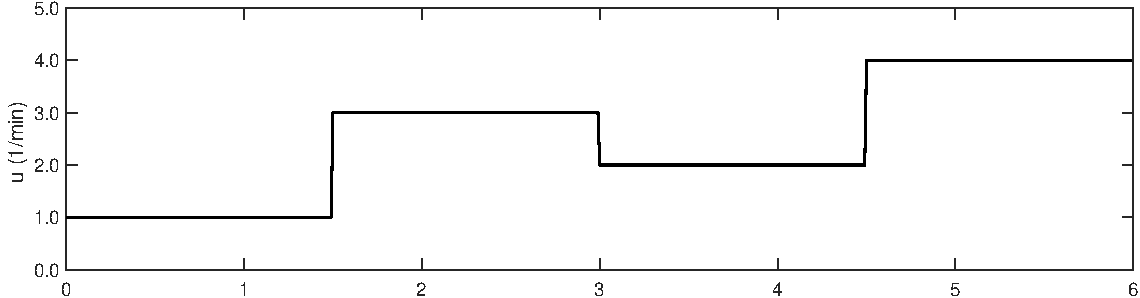
\includegraphics[width=\textwidth]{chapter2/linResp_1_1}};
    	\node [below of=img, node distance=5.5em] (xlabel) {\footnotesize Time (min)};
   	\end{tikzpicture}
	\end{subfigure} \\
    \begin{subfigure}{0.9\textwidth}
    	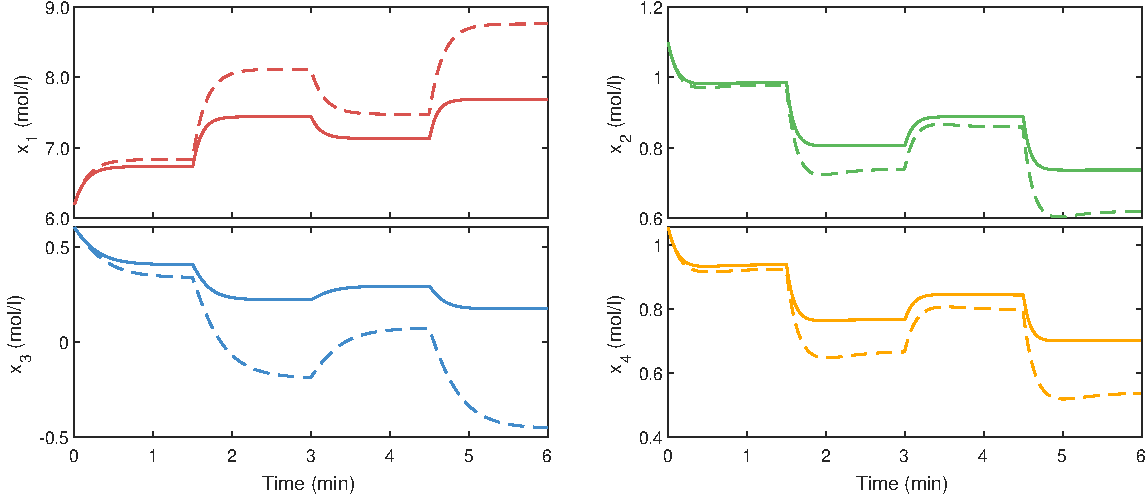
\includegraphics[width=\textwidth]{chapter2/linResp_1_2}
	\end{subfigure}
	
    \caption{Comparison between the nonlinear and linear response of the reactor system.}
    \label{fig:linResp01}
\end{figure}

\section{Response Analysis in the Time Domain}

Once that a model is well-established, it is possible both to simulate the system and to analyze its response, given an initial state and input signal. This section focus on developing a quantitative understanding of a system behavior through a linear model. The results are focused on continuous-time response of linear and time-invariant systems in the form:
\begin{align}
\begin{cases}
    \dot{\bm{x}}(t) = \bm{A} \bm{x}(t) + \bm{B} \bm{u}(t) \\
    \bm{y}(t) = \bm{C} \bm{x}(t) + \bm{D} \bm{u}(t)
\end{cases}
.\end{align}

First of all, it is necessary to access some properties of the matrix $\bm{A}$, which describes the influence of the states in the evolution of the system. Consider, in this case, the following matrix defined by computing the exponential of the matrix $\bm{A}$. 	

\begin{boxed-definition}{(State-Transition Matrix)} \label{def:stateTransM}
    Consider a system in State-Space representation with matrix $\bm{A} \in \mathbb{R}^{n \times n}$. Its \textit{State-Transition Matrix}, $e^{\bm{A} t} \in \mathbb{R}^{n \times n}$ , is the converging series:
\begin{equation}
    e^{\bm{A} t} = \bm{I} + \bm{At} + \cfrac{\bm{A}^2 t^2}{2!} + \cfrac{\bm{A}^3 t^3}{3!} + \cdots = \sum_{k=0}^{\infty} \cfrac{A^k t^k}{k!}
.\end{equation} 
\end{boxed-definition}

This matrix is central to the computation of the system time response, since it can directly relate the initial state of a system to any other state forward in time \textbf{[reference?]}. Moreover, the exponential of a matrix is not a trivial operation. However, the fact that the State-Space matrix $\bm{A}$ is always a square matrix results in the following properties for the State-Transition matrix, stated below.

\begin{boxed-theorem}{} \label{th:stateTransMProp}
    Consider a matrix exponential as in Definition \ref{def:stateTransM}, for a matrix $\bm{A}  \in \mathbb{R}^{n \times n}$. Then, the following properties holds:
\begin{align}
        {\rm I})\ \cfrac{d ( e^{\bm{A} t} )}{dt} = \bm{A} e^{\bm{A} t}; & &
        {\rm II})\ e^{\bm{A} t} e^{\bm{A} \tau} = e^{\bm{A} (t + \tau)}; & &
        {\rm III})\ e^{-\bm{A} t} e^{\bm{A} t} = e^{\bm{A} t} e^{-\bm{A} t}; = \bm{I}
.\end{align}
\end{boxed-theorem}

The proof of these properties can be obtained directly from using the Definition \ref{def:stateTransM} and doing some algebra. Given these results, the calculation of the time response of a system in SS representation becomes straightforward.

\begin{boxed-theorem}{(Lagrange Formula)} \label{th:lagrangeForm}
    Consider a LTI system in State-Space representation. Its response for any time $t \geq t_0$, initial state $\bm{x}(t_0)$ and input signal $\bm{u}(t)$ is given by the solutions of the state and output equations:
    \begin{align}
    \begin{cases}
        \bm{x}(t) = e^{\bm{A}(t - t_0)} \bm{x}(t) + \int_{t_0}^{t} e^{\bm{A}(t - \tau)} \bm{B} \bm{u}(\tau) d \tau \hfill & \\
        \bm{y}(t) = \bm{C} e^{\bm{A}(t - t_0)} \bm{x}(t) + \bm{C} \int_{t_0}^{t} e^{\bm{A}(t - \tau)} \bm{B} \bm{u}(\tau) d \tau + \bm{D} \bm{u}(t) &
    \end{cases}
    .\end{align}
\end{boxed-theorem}

\begin{proof}
    First of all, consider a system in State-Space representation with state equation as defined in \eqref{eq:SSRepr03}. Multiplying both sides by $e^{-\bm{A} t}$:
    \begin{equation} \label{eq:lagrTH01}
    \begin{split}
        e^{-\bm{A} t} \dot{\bm{x}}(t) &= e^{-\bm{A} t} (\bm{A} \bm{x}(t) + \bm{B} \bm{u}(t)) \\
        e^{-\bm{A} t} \dot{\bm{x}}(t) - \bm{A}e^{-\bm{A} t} \bm{x}(t)  &=  e^{-\bm{A} t} \bm{B} \bm{u}(t)
    \end{split}
    .\end{equation}
    
\noindent Using the multiplication rule and the first property from Theorem \ref{th:stateTransMProp}, it is easy to see that $d[e^{-\bm{A} t} \bm{x}(t)]/dt = e^{-\bm{A} t} \dot{\bm{x}}(t) - \bm{A} e^{-\bm{A} t} \bm{x}(t)$. Substituting this result in \eqref{eq:lagrTH01} and integrating both sides from $t_0$ to $t$:
    \begin{equation} \label{eq:lagrTH02}
    \begin{split}
        \cfrac{d(e^{-\bm{A} t} \bm{x}(t))}{dt} &= e^{-\bm{A} t} \bm{B} \bm{u}(t) \\
        \left. e^{-\bm{A} t} \bm{x}(t) \right|^{t}_{t_0}  &= \int_{t_0}^{t} e^{-\bm{A} \tau} \bm{B} \bm{u}(\tau) d\tau \\
        e^{-\bm{A} t} \bm{x}(t) - e^{-\bm{A} t_0} \bm{x}(t_0)  &= \int_{t_0}^{t} e^{-\bm{A} \tau} \bm{B} \bm{u}(\tau) d\tau
    \end{split}
    .\end{equation}
    
\noindent Multiplying both sides of \eqref{eq:lagrTH02} by $e^{\bm{A} t}$ and using the second and third property from Theorem \ref{th:stateTransMProp}, the state response can be calculated as:
    \begin{equation} \label{eq:lagrTH03}
    \begin{split}
        e^{\bm{A} t} \left( e^{-\bm{A} t} \bm{x}(t) \right. &- \left. e^{-\bm{A} t_0} \bm{x}(t_0) \right) = e^{\bm{A} t} \int_{t_0}^{t} e^{-\bm{A} \tau} \bm{B} \bm{u}(\tau) d\tau \\
        \bm{I} \bm{x}(t) &- e^{\bm{A} (t - t_0)} \bm{x}(t_0) = \int_{t_0}^{t} e^{\bm{A}(t - \tau)} \bm{B} \bm{u}(\tau) d\tau \\
        \bm{x}(t) &= e^{\bm{A} (t - t_0)} \bm{x}(t_0) + \int_{t_0}^{t} e^{\bm{A}(t - \tau)} \bm{B} \bm{u}(\tau) d\tau \\
    \end{split}
    .\end{equation}
    
\noindent Finally, substituting \eqref{eq:lagrTH03} into the output equation leads to:
    \begin{equation} \label{eq:lagrTH04}
    \begin{split}
        \bm{y}(t) &= \bm{C} \left( e^{\bm{A} (t - t_0)} \bm{x}(t_0) + \int_{t_0}^{t} e^{\bm{A}(t - \tau)} \bm{B} \bm{u}(\tau) d\tau \right) + \bm{D} \bm{u}(t) \\ 
         &= \bm{C} e^{\bm{A}(t - t_0)} \bm{x}(t) + \bm{C} \int_{t_0}^{t} e^{\bm{A}(t - \tau)} \bm{B} \bm{u}(\tau) d \tau + \bm{D} \bm{u}(t) 
    \end{split}
    .\end{equation}
\end{proof}

When discussing the response of a system, the focus is directed to the state equation describing its dynamics, since the output equation represents an observation of the system through the states. In this sense, the Lagrange formula shows the nice characteristic of linear systems that the total response is a composition of two separated actions:
\begin{equation}
    \bm{x}(t) = \bm{x}_{\text{n}}(t) + \bm{x}_{\text{f}}(t) 
,\end{equation}

\noindent where the natural response, $\bm{x}_{\text{n}}(t)$, corresponds to the state-transition matrix multiplication term and the forced response, $\bm{x}_{\text{f}}(t)$, corresponds to the integral term. This concept is visualized in Fig. \ref{fig:linResp02} for the total response of the first two states of the model derived in \eqref{eq:isoReact01}, given the operation points $\bm{x}_o = [6.19, 1.09]$ and $u_o = 3.03$, excited with a step input $u(t) = 3$, $t \in [0, 1.2]$. In this plot, the solid line represents the total response, whereas the dashed and dotted lines represents the natural and forced response, respectively. It is easy to verify that the decomposition of the total response is equal to the sum of those independent components.

\begin{figure}[ht] \centering
    \begin{subfigure}{0.46\textwidth}
    	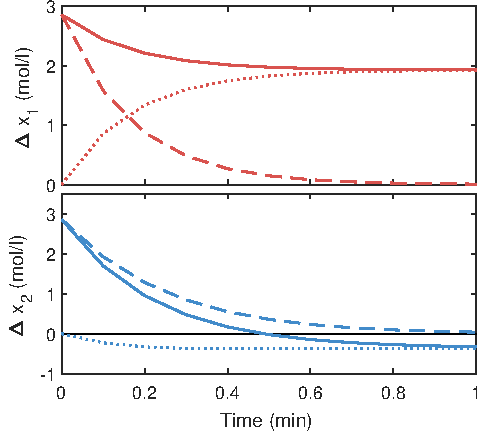
\includegraphics[width=\textwidth]{chapter2/linResp_2_1}
   	\end{subfigure} \hfill
    \begin{subfigure}{0.50	\textwidth}
    	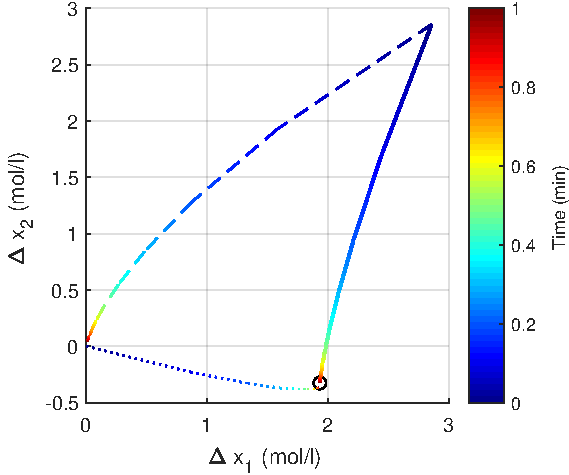
\includegraphics[width=\textwidth]{chapter2/linResp_2_2}
   	\end{subfigure}

    \caption{Simulation of the total response decomposition for the two first states of the model from \eqref{eq:isoReact01}. Each state response is shown separately (left) and together into a trajectory visualization (right), in which the steady-state point is indicated by a circle.}
    \label{fig:linResp02}
\end{figure}

In order to characterize the dynamical response of a system, there is still the need to compute the state-transition matrix. This can be done in several ways \cite{Moler_VanLoan:2003}. A specific method, known as the \textit{Sylvester expansion}, is an analytical solution that brings an understanding of the system behavior through the eigenvalues of the state-state matrix $\bm{A}$.

\begin{boxed-theorem}{(Sylvester expansion)} \label{th:sylvester01}
    Consider a matrix exponential function $e^{\bm{A} t}$ for any square matrix $\bm{A} \in \mathbb{R}^{n \times n}$, whose distinct eigenvalues are $\bm{\lambda} \in \mathbb{R}^{m},\ m \leq n,$ with associated multiplicity vector $\bm{\nu} \in \mathbb{R}^m$ such that $\| \bm{\nu} \|_1 = n$. The result of this function can be expanded as
    \begin{equation} \label{eq:sylvester01}
        e^{\bm{A} t} = \beta_0(t) \bm{I} + \beta_1(t) \bm{A} + \beta_2(t) \bm{A}^2 + ... + \beta_{n-1}(t) \bm{A}^{n-1} = \sum_{i=0}^{n-1} \beta_i(t) \bm{A}^i
    ,\end{equation} 
    
    \noindent where $\beta_i(t) : \mathbb{R} \rightarrow \mathbb{R}$, $i \in [1,2,...,n-1]$, are scalar functions of time. These functions are obtained by solving the linear system
    \begin{equation} \label{eq:sylvester02}
        \bm{V} \bm{\beta} = \bm{\eta}
    ,\end{equation} 
    
    \noindent for the parameter vector $\bm{\beta} = [\beta_0(t), \beta_1(t), ..., \beta_{n-1}(t)]^T$, given vector of modes $\bm{\eta} = [\eta_1, \eta_2, ..., \eta_m]^T$ such that
    \begin{align*}
        \eta_i & = \begin{bmatrix} e^{\lambda_i t} & te^{\lambda_i t} & t^2e^{\lambda_i t} & \cdots & t^{\nu_i-1}e^{\lambda_i t} \end{bmatrix}^T \\
    \end{align*}
    
	\noindent and the confluent Vandermonde matrix $\bm{V} = [V_1, V_2, ..., V_m]^T$ such that
    \begin{align*}
        V_j     & = \begin{bmatrix}
            1 & \lambda_j & \lambda_j^2 & \cdots & \lambda_j^{(\nu_j - 1)} & \cdots & \lambda_j^{n-1} \\
            0 & 1 & 2\lambda_j & \cdots & (\nu_j - 1) \lambda_j^{(\nu_j - 1)} & \cdots & (n-1)\lambda_j^{n-2} \\
            \vdots & \vdots & \vdots & \ddots & \vdots & \ddots & \vdots \\
            0 & 0 & 0 & \cdots & (\nu_j - 1)! & \cdots & \cfrac{(n - 1)!}{(n - \nu_j)!}\lambda_j^{n-\nu_j} \\
        \end{bmatrix}\
    \end{align*} 
\end{boxed-theorem}

The proof of this expansion is somewhat extensive, but a detailed discussion can be found in \cite{Chen:1998}. Basically, the expansion in \eqref{eq:sylvester01} is a direct application of the Cayley-Hamilton theorem \cite{Atiyah:2018} and the linear system in \eqref{eq:sylvester02} is a result of the Sylvester's matrix theorem \cite{Horn:2012}.

From the expansion presented in Theorem \ref{th:sylvester01}, it is possible to understand the relationship between the state-transition matrix $e^{\bm{At}}$ and each eigenvalue $\lambda$ of the matrix $\bm{A}$, also known as the \textit{poles} of the system. First of all, notice that the formulation of the linear system that defines the parameters $\beta_0(t), \beta_1(t), ..., \beta_{n-1}(t)$ implies that each one of these functions are linear combinations of the exponentials $e^{\lambda_i t}$ for each eigenvalue $\lambda_i,\ i=1,2,...m$. These exponentials are known as the \textit{modes} of the matrix $\bm{A}$. Since the Sylvester expansion is linear in those parameters, it is possible to conclude that the state-transition matrix, and consequently the response of a system, is a linear combination of the modes.

\begin{boxed-example}{} \label{ex:stateTrans}
	Consider, for the sake of illustration, the same State-Space model as the one simulated in Fig. \ref{fig:linResp01}, but considering only the first two states (since they are independent of the others). Its matrix $\bm{A}$ is shown below:
	\begin{align} \label{eq:stateRespEx01}
	    \bm{A} = \begin{bmatrix} 
	        -5.93  &        0 \\
	        0.83   &  -4.70 
	    \end{bmatrix}
	.\end{align}
	
\noindent It is easy to see that $\bm{\lambda} = [-5.93, -4.70]$, since $\bm{A}$ is diagonal. The Sylvester expansion for the exponential of this matrix has the parameter vector $\bm{\beta} = [\beta_0(t), \beta_1(t)]$ which solves the system
	\begin{align}
	\begin{bmatrix}
		1 & -5.93 \\ 1 & -4.70
	\end{bmatrix} \begin{bmatrix}
		\beta_0(t) \\ \beta_1(t)
	\end{bmatrix} = \begin{bmatrix}
		e^{-5.93 t} \\ e^{-4.70 t}
	\end{bmatrix}
	.\end{align}
	
	\noindent The solution to this system is $\bm{\beta} = [4.82e^{-4.7t}-3.82e^{-5.93t},\ 0.813e^{-4.7t} - 0.813e^{-5.93t}]$. Hence, state-transition matrix is calculated through the expansion:
	\begin{align}
	\begin{split}
		e^{\bm{A} t} & = \beta_0(t) \bm{I} + \beta_1(t) \bm{A} \\ & = 4.82e^{-4.7t}-3.82e^{-5.93t} \begin{bmatrix} 1 & 0 \\ 0 & 1 \end{bmatrix} + 0.813e^{-4.7t}-0.813e^{-5.93t} \begin{bmatrix} -5.93  & 0 \\ 0.83  & -4.70 \end{bmatrix} \\
		& =  \begin{bmatrix} e^{-5.93t} & 0 \\ 0.675e^{-4.7t} - 0.675e^{-5.93t} & e^{-4.7t} \end{bmatrix} \\
	\end{split}
	.\end{align}
\end{boxed-example}

The simulation in Fig \ref{fig:stateTrans01} shows the evolution of each element of the state-transition matrix from Example \ref{ex:stateTrans}, for a given time interval. Considering only the natural response $\bm{x}_n(t)$, i.e., setting $\bm{u}(t) = \bm{0},\ t \in [t_0, t]$, it is evident from the Lagrange formula that the time evolution of each state is given by a row-wise weighted sum of these elements. The weights, in this case, are given by the initial state $\bm{x}(t_0)$. Therefore, the $(i, j)$ element of this matrix describes how the $j$-th state affects the response of the $i$-th state.

\begin{figure}[ht] \centering
    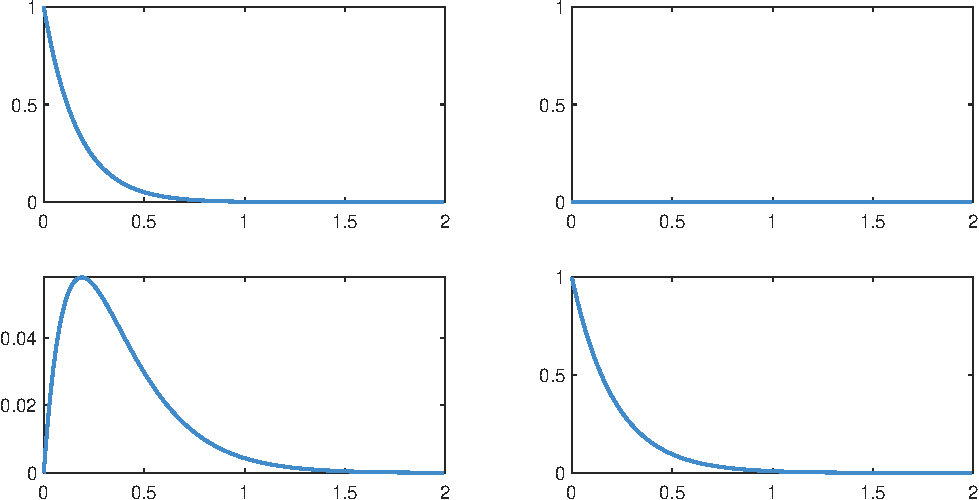
\includegraphics[width=\textwidth]{chapter2/stateTrans01}
    
    \caption{Simulation of the state-transition matrix $e^{\bm{A} t}$ from Example \ref{ex:stateTrans} for $t \in [0, 1.5]$.}
    \label{fig:stateTrans01}
\end{figure}

Now, attention must be drawn to the case where the eigenvalues are not real, but complex and conjugate. Despite that the Sylvester expansion is still defined as in Theorem \ref{th:sylvester01}, this case introduces a slightly different interpretation of the modes contributions to the natural response.

\begin{boxed-theorem}{} \label{th:sylvester02}
    Consider the same expansion defined in Theorem \ref{th:sylvester01}. Consider, now, that the matrix $\bm{A}$ has two distinct eigenvalues $\lambda_c, \lambda_c' \in \mathbb{C}$ in the form $\lambda_c, \lambda_c' = \alpha \pm j \omega$. In this case, the linear system solved by the parameters $\beta_0(t), \beta_1(t), ..., \beta_{n-1}(t)$ will have two equations:
    \begin{align} \label{eq:sylvEq01}
    \begin{cases}
        \beta_0 + \alpha \beta_1 + \alpha^{2} \beta_2 + ... + \alpha^{n-1} \beta_{n-1} = e^{\alpha t} cos(\omega t) & \\
        \hfill 0 + \omega \beta_1 + \omega^{2} \beta_2 + ... + \omega^{n-1} \beta_{n-1} = e^{\alpha t} sin(\omega t) &
    \end{cases}
    .\end{align}
\end{boxed-theorem}

\begin{proof}
    Consider the matrix $\bm{A}$ with eigenvalues as specified and the Sylvester expansion as presented. In this case, there will be two equations in the system:
    \begin{align} 
    \begin{cases}
        \beta_0 + \lambda_c \beta_1 + \lambda_c^2  \beta_2 + ... + \lambda_c^{n-1} \beta_{n-1} = e^{\lambda_c t} & \\
        \beta_0 + \lambda_c' \beta_1 + (\lambda_c')^{2} \beta_2 + ... + (\lambda_c')^{n-1} \beta_{n-1} = e^{\lambda_c' t} &
    \end{cases}
    .\end{align}
    
    Since the eigenvalues are complex and conjugate, it has that $\lambda_c + \lambda'_c = 2 \mathbb{R}e[\lambda_c] = 2 \alpha$ and $\lambda_c - \lambda'_c = 2j \mathcal{I}m[\lambda_c] = 2j \omega$. Moreover, the Euler identity $e^{\alpha \pm j \omega} = e^{\alpha t}(cos(\omega) \pm j sin(\omega))$ shows that $e^{\lambda} + e^{\lambda'} = 2 e^{\alpha t} cos(\omega t)$ and $e^{\lambda} - e^{\lambda'} = 2 e^{\alpha t} sin(\omega t)$. In this case, summing the two rows and subtracting the first row by the second one results in:
    \begin{align} 
    \begin{cases}
        \beta_0 + 2 \alpha \beta_1 + 2 \alpha^2  \beta_2 + ... + 2 \alpha^{n-1} \beta_{n-1} = 2 e^{\alpha t} cos(\omega t) & \\
        0 + 2j \omega \beta_1 + 2j \omega^{2} \beta_2 + ... + 2j \omega^{n-1} \beta_{n-1} = 2j e^{\alpha t} sin(\omega t) &
    \end{cases}
    .\end{align}
    
    Finally, dividing the first row by $2$ and the second row by $2j$ results in \eqref{eq:sylvEq01}.
\end{proof}

From the same reasons stated before, this result implies that the actual response of the system will have sinusoidal components that produces oscillations in the response. The modes associated with complex and conjugate eigenvalues are classified as \textit{pseudo-periodic}, since they are composed by an exponential growth (or decay) enveloping a sinusoidal function. 

\begin{boxed-example}{} \label{ex:stateTrans02}
	Consider, again for the sake of illustration, the following example. A toy system is described by the matrix
	\begin{align} \label{eq:stateRespEx02}
	    \bm{A} = \begin{bmatrix} 
	         -0.1  &  \hfill 0.5 \\
	        -0.5   &  -0.1 
	    \end{bmatrix}
	.\end{align}
	
	\noindent The eigenvalues of this matrix are given as $\lambda, \lambda' = -0.1 \pm j0.5$. The Sylvester expansion for the exponential of this matrix has the parameter vector $\bm{\beta} = [\beta_0(t), \beta_1(t)]$ which solves the system
	\begin{align}
	\begin{bmatrix}
		1 & -0.1 \\ 0 & \phantom{-} 0.5
	\end{bmatrix} \begin{bmatrix}
		\beta_0(t) \\ \beta_1(t)
	\end{bmatrix} = \begin{bmatrix}
		e^{-0.1t} cos(0.5 t) \\ e^{-0.1t} sin(0.5 t)
	\end{bmatrix}
	.\end{align}
	
	\noindent The solution to this system is $\bm{\beta} = [e^{-0.1t}cos(0.5 t) + 0.2e^{-0.1 t} sin(0.5 t),\ 2 e^{-0.1 t} sin(0.5 t)$. Hence, state-transition matrix is calculated through the expansion:
	\begin{align}
	\begin{split}
		e^{\bm{A} t} & = \beta_0(t) \bm{I} + \beta_1(t) \bm{A} \\ & = e^{-0.1t}cos(0.5 t) + 0.2e^{-0.1 t} sin(0.5 t) \begin{bmatrix} 1 & 0 \\ 0 & 1 \end{bmatrix} + 2 e^{-0.1 t} sin(0.5 t) \begin{bmatrix} -0.1  & 0.5 \\ -0.5  & -0.1 \end{bmatrix} \\
		& =  \begin{bmatrix} \phantom{-}e^{-0.1t} cos(0.5 t) & e^{-0.1t} sin(0.5 t) \\ -e^{-0.1t} sin(0.5 t) & e^{-0.1t} cos(0.5 t) \end{bmatrix} \\
	\end{split}
	.\end{align}
\end{boxed-example}
	
The elements of the resulting state-transition matrix are shown in Fig. \ref{fig:stateTrans02}. It is possible to see, in this case, the pseudo-periodic behavior of the complex conjugate modes, where the dashed lines represents the exponential envelope. 

\begin{figure}[ht] \centering
    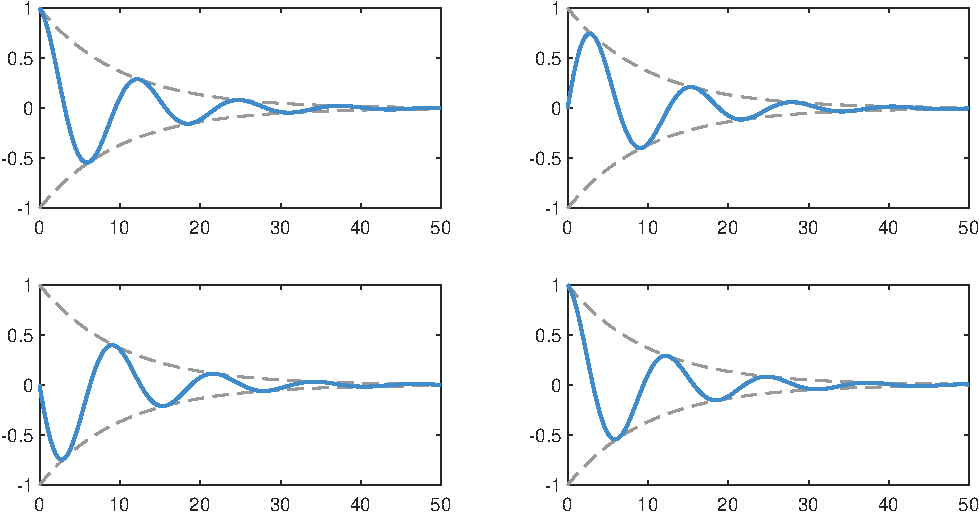
\includegraphics[width=\textwidth]{chapter2/stateTrans02}
    
    \caption{Simulation of the state-transition matrix $e^{\bm{A} t}$ from Example \ref{ex:stateTrans02} for $t \in [0,50]$.}
    \label{fig:stateTrans02}
\end{figure}

The previous discussion on the modes of matrix $\bm{A}$ introduced the importance of the eigenvalues of this matrix in analyzing the system response. The analysis, however, focused on the natural response $\bm{x}_n(t)$, whereas the forced response $\bm{x}_f(t)$ was deliberately omitted. Now, the analysis focus on the opposite case. Consider the two systems described by the matrices $(\bm{A}^{(1)}, b^{(1)})$ and $(\bm{A}^{(2)}, b^{(2)})$ given below. These matrices are more complete descriptions of the systems from Examples \ref{ex:stateTrans} and \ref{ex:stateTrans02}. 
\begin{equation} \label{eq:isoSys02}
\begin{matrix}
    \bm{A}^{(1)} = \begin{bmatrix} 
        -5.93  &      0 \\
        \hfill 0.83   &  -4.70 
    \end{bmatrix} & b^{(1)} = \begin{bmatrix} \phantom{-}3.81 \\ -1.09 \end{bmatrix}; & & \bm{A}^{(2)} = \begin{bmatrix} 
         -0.1  &  \hfill 0.5 \\
        -0.5   &  -0.1 
    \end{bmatrix} & b^{(2)} = \begin{bmatrix} 1 \\ 1 \end{bmatrix}
\end{matrix}
.\end{equation}

Considering initial states $\bm{x}^{(1)}(0) = \bm{x}^{(2)}(0) = \bm{0}$ and the input signals $\bm{u}^{(1)}(t) = \bm{u}^{(2)}(t) = \bm{1}$, for time $t \in [0, 60]$, the evolution of the first state of both systems are shown in Fig. \ref{fig:forcedResponse}. Since $\bm{A}^{(1)}$ is diagonal and $\bm{A}^{(2)}$ has a pair of complex conjugate eigenvalues, it is possible to consider that those are characteristic responses of aperiodic and pseudo-periodic modes, respectively, to an unitary step input signal.

\begin{figure}[ht] \centering
    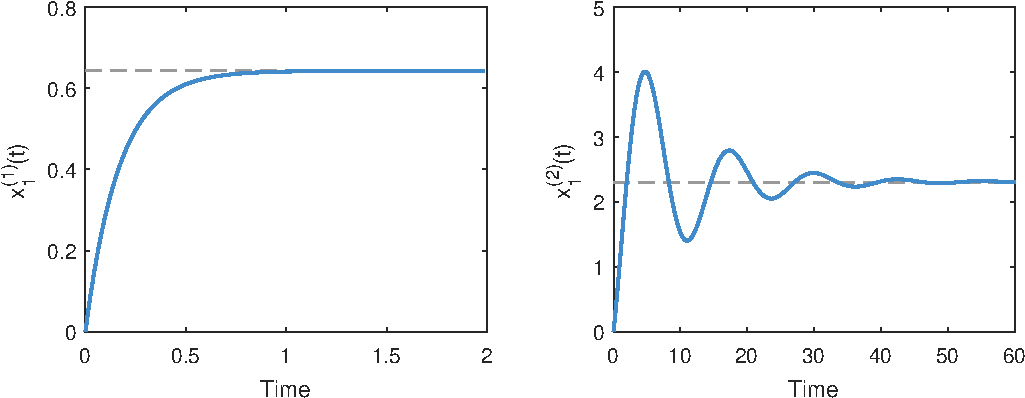
\includegraphics[width=\textwidth]{chapter2/forcedResponse}
    
    \caption{One-state forced response of the two systems from \eqref{eq:isoSys02}.}
    \label{fig:forcedResponse}
\end{figure}

The unitary step is the default input signal used to analyze the forced response of dynamical systems. This is due to the fact that any continuous signal can be approximated by a sequence of step signals. When discussing the time evolution of systems given forcing input signals, the response can be separated into a transient regime and a subsequent steady-state regime. The transient part of the response corresponds to the dynamical evolution from the previous state equilibrium to the next steady-state point. The steady-state point, as already mentioned, corresponds to the point in which the derivatives of the states are zero, which represents the discharge of the initial energy given by the forcing input. These regimes can be characterized in respect to the specifications given below.

\begin{boxed-definition}{(Unit-Step Response Specifications)} \label{def:responseParameters}
    Given a mode $e^{\lambda t}$ associated with the eigenvalue $\lambda \in \mathbb{R}$, its contribution to the response has a time constant ($\tau$) defined as
    \begin{equation}
        \tau = - \cfrac{1}{\lambda}
    .\end{equation}  
    
    Furthermore, given pseudo-periodic modes $e^{\lambda t}$ and $e^{\lambda' t}$ associated with the eigenvalues $\lambda,\lambda' = \alpha \pm j \omega$ of a matrix $\bm{A}$, their contribution to the response has a time constant ($\tau$), a natural frequency ($\omega_n$) and a damping coefficient ($\zeta$) defined as:
    \begin{equation}
    \begin{matrix}
        \tau = - \cfrac{1}{\alpha} &; & & \omega_n = \sqrt{\alpha^2 + \omega^2} &; & & \zeta = - \cfrac{\alpha}{\omega_n}
    \end{matrix}
    .\end{equation}
    
\end{boxed-definition}   

The specifications just defined provides a quantitative way to describe the response of a system in terms of time and frequencies. The time constant, for instance, is a quantity that represents the time needed for the mode to lost $63\%$ of its initial value, since $e^{\lambda \tau} = e^{-1} = 0.37$. A greater value of a time constant indicates that the system is able to ``discharge" energy faster. The damping coefficient, in turn, provides an information about the intensity of the peak in the pseudo-periodic responses, which is known as \textit{overshoot} (or \textit{undershoot} in the case of a negative peak) and the natural frequency represents the oscillation of the response before reaching steady-state. From the perspective of control theory, these are some of the specifications used to define desirable transient responses to a controlled system.

Notice that the response specifications are always functions of the real and imaginary parts of the eigenvalues. This brings the possibility of a visualization in the complex plane to interpret how each eigenvalue contributes to the total response. A straightforward notion is that the closer an eigenvalue is to the imaginary axis, the faster is its contribution. Similarly, the furthest an eigenvalue is to the real axis, the more oscillatory is its contribution. Finally, a vector from the origin of the plane to a complex eigenvalue has a norm equal to the natural frequency ($\omega_n$) and the cosine of the angle formed with the imaginary axis is equal to the damping factor ($\zeta$). A simulation of the contributions from different eigenvalues are shown in Fig. \ref{fig:eigen01}.

\begin{figure}[ht]  \centering
    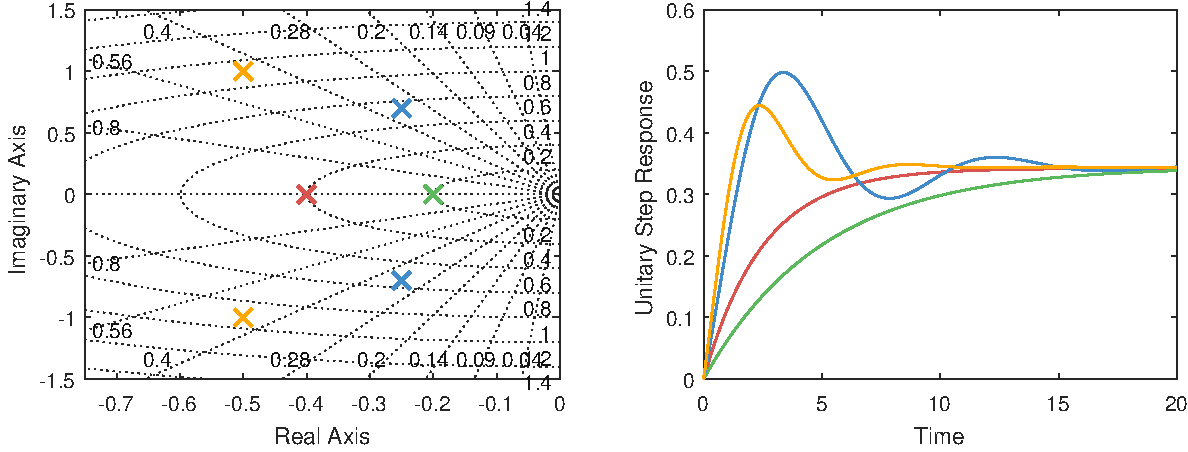
\includegraphics[width=\textwidth]{chapter2/eigen01}
    
    \caption{Eigenvalues of a system and the forced response associated with their modes.}
    \label{fig:eigen01}
\end{figure}

\section{Similarity Transformations}

A State-Space representation can be interpreted through a system of coordinates. A state, in this context, represents a point as visualized through this reference. Under the assumption of a linear time-invariant system, there is an intuition that is possible to change the representation of the states by changing this system of coordinates through some linear transformation, obtaining a different representation to the same system. This is the motivation for this section.

First of all, consider a brief reflection about the geometrical interpretation of a State-Space model. Let any state-vector at an arbitrary time $t$ be $\bm{x}(t)$, defined in the $\mathbb{R}^{2}$ space. Naturally, it is possible to associate to this vector an orthonormal basis $\bm{I} \in \mathbb{R}^2$, the 2-dimensional identity matrix. There is, however, the possibility to associate any other arbitrary basis to represent a state-vector and visualize both states through this new perspective. When the basis is not orthogonal, a change in the state-vector in a direction parallel to a component of the basis, i.e., a change in only one element of this vector, also produces a change in other directions if observed through the original orthonormal basis. This is an interesting result, since it allows for the use of a single direction to represent the simultaneous evolution of both states.

In the State-Space formulation, the matrix $\bm{A}$ represents a linear function that maps state-vectors from $\mathbb{R}^{n}$ to itself. When applying a new basis to represent the state-vectors, it is intuitive that the mapping performed by this function also changes so that it still represents the same linear combination of the states.

\begin{boxed-theorem}{(Similarity Transformation)}
    Consider a system in SS representation described by the matrices $(\bm{A}, \bm{B}, \bm{C}, \bm{D})$ and a nonsingular transformation matrix $\bm{P} \in \mathbb{R}^{n \times n}$. An equivalent representation for the transformation $\bm{z}(t) = \bm{P} \bm{x}(t)$ is:
    \begin{align}
    \begin{cases}
        \dot{\bm{z}}(t) = \tilde{\bm{A}} \bm{z}(t) + \tilde{\bm{B}} \bm{u}(t) & \\
        \bm{y}(t) = \tilde{\bm{C}} \bm{z}(t) + \tilde{\bm{D}} \bm{u}(t)
    \end{cases} 
    ,\end{align}
    
    \noindent where:
    \begin{equation}
        \begin{matrix}
            \tilde{\bm{A}} = \bm{P} \bm{A} \bm{P}^{-1} &; & \tilde{\bm{B}} = \bm{P} \bm{B} &; & \tilde{\bm{C}} = \bm{C} \bm{P}^{-1} &; & \tilde{\bm{D}} = \bm{D}
        \end{matrix}
    .\end{equation}
\end{boxed-theorem}

\begin{proof}
    Consider a SS representation and any nonsingular matrix $\bm{P} \in \mathbb{R}^{n \times n}$. Making $\bm{z}(t) = \bm{P} \bm{x}(t)$ leads to $\bm{x}(t) = \bm{P}^{-1} \bm{z}(t)$. Substituting this in the state equation results in:
    \begin{equation}
    \begin{split}
        \dot{\bm{x}}(t) &= \bm{A} \bm{x}(t) + \bm{B} \bm{u}(t) \\
        \bm{P}^{-1} \dot{\bm{z}}(t) &= \bm{A} \bm{P}^{-1} \bm{z}(t) + \bm{B} \bm{u}(t) \\
        \bm{I} \dot{\bm{z}}(t) &= \bm{P} \bm{A} \bm{P}^{-1} \bm{z}(t) + \bm{P} \bm{B} \bm{u}(t) \\
        \dot{\bm{z}}(t) &= \tilde{\bm{A}} \bm{z}(t) + \tilde{\bm{B}} \bm{u}(t)
    \end{split}
    .\end{equation}
    
    Thus, substituting $\bm{x}(t) = \bm{P}^{-1} \bm{z}(t)$ in the output equation results in:
    \begin{equation}
    \begin{split}
        \bm{y}(t) &= \bm{C} \bm{x}(t) + \bm{D} \bm{u}(t) \\
        	&= \bm{C} \bm{P}^{-1} \bm{y}(t) + \bm{D} \bm{u}(t) \\
        	&= \tilde{\bm{C}} \bm{z}(t) + \tilde{\bm{D}} \bm{u}(t)
    \end{split}
    .\end{equation}
\end{proof}

By this theorem is it clear that, after transforming the state-vector, the entire dynamical model $(\bm{A}, \bm{B}, \bm{C}, \bm{D})$ changes. This would imply that the analysis of the original system, for its properties and time response, is not valid for the similar transformed system. However, as discussed before, these transformations accounts for the same system when observed through a different reference basis. Therefore, it is expected that the model presents the same analysis results, as demonstrated below.

\begin{boxed-theorem}{} \label{th:simTrans01}
    Consider a system in State-Space form with matrix $\bm{A}$. Consider also a similarity transformation $\bm{z}(t) = \bm{P} \bm{x}(t)$ that results in a matrix $\tilde{\bm{A}} = \bm{P} \bm{A} \bm{P}^{-1}$. In this case, $\bm{A}$ and $\tilde{\bm{A}}$ shares the same set of eigenvalues.
\end{boxed-theorem}

\begin{proof}
    The eigendecomposition problem is defined as $\bm{A} \bm{v} = \bm{\lambda} \bm{v}$. From the similarity transformation, $\tilde{\bm{A}} = \bm{P} \bm{A} \bm{P}^{-1}$ leads to $\bm{A} = \bm{P}^{-1} \tilde{\bm{A}} \bm{P}$. Substituting this in the eigendecomposition:
    \begin{align}
    \begin{split}
        \bm{P}^{-1} \tilde{\bm{A}} \bm{P} \bm{v} & = \bm{\lambda} \bm{v} \\
        \tilde{\bm{A}} \bm{P} \bm{v} & =  \bm{\lambda} \bm{P} \bm{v}
    \end{split}
    .\end{align}
   
    Considering the transformed eigenvector $\tilde{\bm{v}} = \bm{P} \bm{v}$, it is clear that $\tilde{\bm{A}} \tilde{\bm{v}} = \bm{\lambda} \tilde{\bm{v}}$. This implies that matrices $\bm{A}$ and $\tilde{\bm{A}}$ shares the same set of eigenvalues $\bm{\lambda}$.
\end{proof}

It is clear from previous results that, since both the matrices shares the same set of eigenvalues, the original and transformed model provides the same dynamical responses and, as shown later, the same general dynamic properties. Therefore, the similarity transformation consists in a method to produce new State-Spaces representations that emphasizes some geometrical perspective of the model, hopefully helping to analyze a specific property, without actually changing the relationship between the original model and the physical system.

The use of similarity transformations can also benefits the computation of functions of the matrices of the State-Space representation, given that they impose a desirable structure to this matrix. With this motivation, a popular transformation that provides a new representation with computational advantages is the Similarity transformation.

\begin{boxed-theorem}{(Diagonalization)}
    Consider a $n$-dimensional system in State-Space form represented by the matrices $(\bm{A}, \bm{B}, \bm{C}, \bm{D})$. Let matrix $\bm{A}$ have $n$ distinct real eigenvalues, i.e., $\bm{\lambda} \in \mathbb{R}^n$. Performing the transformation $\bm{z}(t) = \bm{V} \bm{x}(t)$, where $\bm{V} = [\bm{v}_1, \bm{v}_2, ..., \bm{v}_n]$ is the modal matrix composed by the eigenvectors $\bm{v}_i \in \mathbb{R}^n$, $i \in [1, ..., n]$, of matrix $\bm{A}$, will result in a transformed matrix $\bm{\Lambda} = \bm{V} \bm{A} \bm{V}^{-1}$ is diagonal.
\end{boxed-theorem} 

\begin{proof}
    Since the eigenvalues are real and distinct, the eigenvectors must be linearly independent, proving that the inverse $\bm{V}^{-1}$ always exist and that it is a feasible transformation matrix. Using the identity for the eigendecomposition of matrix $\bm{A}$:
    \begin{align}
    \begin{split}
        \bm{\lambda} \bm{v} &= \bm{A} \bm{v} \\
        \begin{bmatrix} \lambda_1 \bm{v}_1 & \lambda_2 \bm{v}_2 & \cdots & \lambda_n \bm{v}_n \end{bmatrix} &= \begin{bmatrix} \bm{A} \bm{v}_1 & \bm{A} \bm{v}_2 & \cdots & \bm{A} \bm{v}_n  \end{bmatrix} \\
        \begin{bmatrix} \bm{v}_1 & \bm{v}_2 & \cdots & \bm{v}_n \end{bmatrix} \begin{bmatrix} \lambda_1 & 0 & \cdots & 0 \\ 0 & \lambda_2 & \cdots & 0 \\ \vdots & \vdots & \ddots & \vdots \\ 0 & 0 & \cdots & \lambda_n  \end{bmatrix} & = \bm{A} \begin{bmatrix} \bm{v}_1 & \bm{v}_2 & \cdots & \bm{v}_n \end{bmatrix} \\
        \begin{bmatrix} \lambda_1 & 0 & \cdots & 0 \\ 0 & \lambda_2 & \cdots & 0 \\ \vdots & \vdots & \ddots & \vdots \\ 0 & 0 & \cdots & \lambda_n  \end{bmatrix} & = \begin{bmatrix} \bm{v}_1 & \bm{v}_2 & \cdots & \bm{v}_n \end{bmatrix}^{-1} \bm{A} \begin{bmatrix} \bm{v}_1 & \bm{v}_2 & \cdots & \bm{v}_n \end{bmatrix} \\
        \bm{\Lambda}  &= \bm{V}^{-1} \bm{A} \bm{V}
    \end{split}
    .\end{align}
    
    Thus, $\bm{\Lambda}$ is a diagonal matrix whose elements are the eigenvalues of matrix $\bm{A}$.
\end{proof}

A model with a diagonal matrix $\bm{A}$ has the nice property that the evolution of the states are decoupled, in the sense that each state evolution is a linear function of itself. A geometrical interpretation of this transformation is that the eigenvectors of this matrix produces a basis that encode information about the interaction between those states, while the interaction in the original formulation was the linear combination of the modes. This result can be easily extended to the case where the eigenvalues are distinct conjugate complex pairs.

In this diagonalization procedure, the elements of the resulting matrix $\bm{\Lambda}$ are the very own eigenvalues of the original matrix $\bm{A}$. Furthermore, it is easy to verify that the state-transition matrix for the transformed matrix, $e^{\bm{\Lambda} t}$, is also a diagonal matrix whose elements are the modes of the system, and can be easily computed as:
\begin{align}
\begin{split}
    e^{\bm{\Lambda} t} & = \sum_{k=0}^{\infty} \cfrac{A^k t^k}{k!   }  = \sum_{k=0}^{\infty} \cfrac{t^k}{k!} \begin{bmatrix} \lambda_1^k & 0 & \cdots & 0 \\ 0 & \lambda_2^k & \cdots & 0 \\ \vdots & \vdots & \ddots & \vdots \\ 0 & 0 & \cdots & \lambda_n^k  \end{bmatrix} = \begin{bmatrix} \displaystyle\sum_{k=0}^{\infty} \cfrac{t^k\lambda_1^k}{k!} & 0 & \cdots & 0 \\ 0 & \displaystyle\sum_{k=0}^{\infty} \cfrac{t^k\lambda_2^k}{k!} & \cdots & 0 \\ \vdots & \vdots & \ddots & \vdots \\ 0 & 0 & \cdots & \displaystyle\sum_{k=0}^{\infty} \cfrac{t^k\lambda_n^k}{k!} \end{bmatrix} \\ 
    &= \begin{bmatrix} e^{\lambda_1 t} & 0 & \cdots & 0 \\ 0 & e^{\lambda_2 t} & \cdots & 0 \\ \vdots & \vdots & \ddots & \vdots \\ 0 & 0 & \cdots & e^{\lambda_n t} \end{bmatrix} .
\end{split}
\end{align}

In the case that the eigenvalues are not all distinct, it may be not possible to design a modal matrix in the same way, since the eigenvectors could not be all linearly independent, and the matrix would not form a basis. In those cases, however, it is still possible to design a generalized modal matrix that transform the original matrix $\bm{A}$ to a quasi-diagonal matrix $\bm{J}$, in which there are decoupled states between blocks. This similarity transformation is known as the Jordan form \cite{Strang:2016}, and it generalizes the notion of diagonalization for any arbitrary matrix.

\section{Stability, Controlability and Observability}

When moving from the dynamical system analysis to a practical perspective of control theory, it is necessary to define and discuss some important properties system and their models. These are definitions concerning the stability, controllability and observability of dynamical systems. Although those properties are established from the dynamical model of the system, they can be directly related to questions about control and measurement instrumentation applied to the control system. .

\subsubsection{Stability}

The first property to be discussed consists in the stability of a system. An instable system, as the name suggests, is a system whose response does not converge to a specific value and rather oscillates or grows unbounded. In physical scenarios, unstable systems are problematic, since their response to external stimuli can result in dangerous situations to itself and, maybe, to the environment around it. Because of this, determining the stability of a system is a crucial procedure into analyzing a system that will be controlled. Under the several quantitative methods to determine if a system is indeed stable, given a mathematical model, a popular and practical one is the Bounded-Input Bounded-Output (BIBO) stability criteria.

\begin{boxed-definition}{(BIBO Stability)} \label{def:BIBOStab}
    A dynamical system is defined as BIBO stable if every bounded input stimuli $| \bm{u}(t) | \leq \epsilon < \infty$ produces in it a bounded output response $| \bm{y}(t) | \leq \delta < \infty$.
\end{boxed-definition}

The main result behind this criteria is that the natural response of a system should vanish as time evolves, i.e., $\bm{x}(t) \to \bm{0}$ as $t \to \infty$. This result is very intuitive from Theorem \ref{th:lagrangeForm}, since the vanishing of the natural response implies that $e^{\bm{A} t} \to \bm{0}$ as $t \to \infty$ and the forced response is expected to be bounded, if $\bm{u}(t)$ is bounded. Since the state-transition matrix is a linear combination of the modes, and the modes are exponential functions of the eigenvalues of the matrix $\bm{A}$, it is possible to determine a condition for stability in the light of these quantities, as shown in the following theorem.

\begin{boxed-theorem}{(BIBO Stability in SS)} \label{th:BIBOStab}
    A system in State-Space form, represented by a matrix $\bm{A} \in \mathbb{R}^{n \times n}$ with eigenvalues $\bm{\lambda} \in \mathbb{R}^n$, is BIBO stable if and only if $\text{Re}[\lambda_i] < 0,\ \forall i \in [1,2,...,n]$.
\end{boxed-theorem}

A detailed proof of this theorem can be found in Appendix A. First of all, note that this criteria depends only on the eigenvalues of matrix $\bm{A}$, so the stability property of a system is invariant to any similarity transformation, since $\bm{A}$ and any transformed matrix $\tilde{\bm{A}} = \bm{P} \bm{A} \bm{P}^{-1}$ shares the same eigenvalues. From the previous results it is also known that the real part of the eigenvalues, independent of their multiplicity or domain, appears as the arguments of the exponential functions that are the system modes. Therefore, an eigenvalue with a negative real part will produce a mode that decays exponentially, as this theorem shows. By the same argument, if the matrix $\bm{A}$ has at least one eigenvalue $\lambda_j = 0$ such that $\mathbb{R}e[\lambda_i] \leq 0,\ \forall i \in [1,2,...,n]$, then the mode associated with this eigenvalue is a constant and the natural response becomes bounded. This configuration is known as a marginally stable condition, in the BIBO perspective. The time response of a $2$-nd order system is shown Fig. \ref{fig:stability01} for three different poles configurations, given an unitary step.

\begin{figure}[ht] \centering
    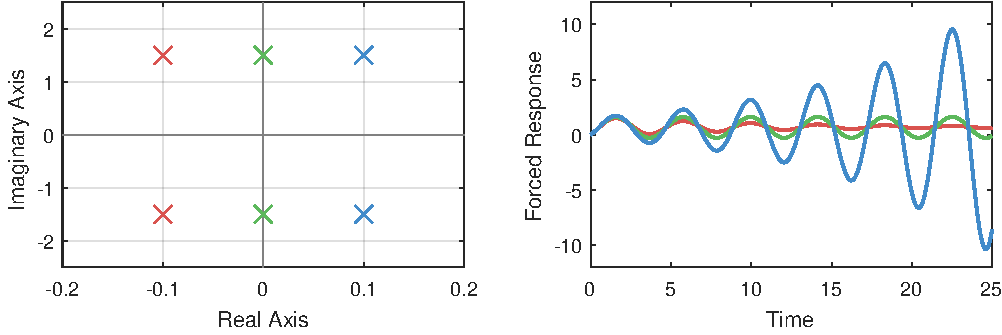
\includegraphics[width=\textwidth]{chapter2/stability01}
    
    \caption{Stability of forced responses given the positions of the system poles.}
    \label{fig:stability01}
\end{figure} 

\subsubsection{Controllability}

Later chapters will discuss the possibility of stabilize an unstable system through a controller. There are, however, some restrictions to the possibility of controlling or not the states of a system, which includes the necessity of discussing \textit{controllability}. The controllability of a system states whether it is possible to calculate an input signal that drives the system to any arbitrary point in the space, in a finite time interval. This property accounts exclusively for this possibility, in the sense that it does not account for the operational feasibility of actually applying this input signal into a physical system, since it may need more energy than an actuator can produce. 

\begin{boxed-definition}{(Controllability)}
    A system in State-Space form with matrices $(\bm{A}, \bm{B})$ is said to be controllable if, for any initial state $\bm{x}(t_0) = \bm{x}_0$ and terminal state $\bm{x}(T) = \bm{x}_T$, $T < \infty$, there exists an input signal $\bm{u}(t)$, $t \in [t_0, T]$, that can transfer $\bm{x}(t_0)$ to $\bm{x}(T)$. Otherwise, the system is said to be uncontrollable. 
\end{boxed-definition}

There are several methods to analyze the controllability of a system given a mathematical model and the definition above. A popular criteria introduces the concept of a controllability matrix and has a nice geometrical interpretation.

\begin{boxed-theorem}{(Controllability in SS)}
    Consider a system in linear State-Space form with matrices $(\bm{A}, \bm{B})$ and the controllability matrix $\bm{\mathcal{C}} \in \mathbb{R}^{n \times nr}$ defined as:
    \begin{equation}
        \bm{\mathcal{C}} = \begin{bmatrix} \bm{B} & \bm{A} \bm{B} & \bm{A}^2 \bm{B} & \cdots & \bm{A}^{n-1} \bm{B} \end{bmatrix}
    .\end{equation}
    
    The system is controllable if and only if $\bm{\mathcal{C}}$ has full row rank.
\end{boxed-theorem}   

An intuition behind this theorem is that the full row rank condition implies that $\mathcal{C}$ has $n$ linearly independent columns, therefore these columns can be used as a basis for what is known as the \textit{controllable subspace}. To better understand that, consider the following forced solution $\bm{x}_f(t)$ given by the Lagrange formula:
\begin{equation} \label{eq:ctrbCayley}
    \bm{x}_f(t) = \int_{0}^{t} e^{\bm{A} (t-\tau)} \bm{B} \bm{u}(\tau) d\tau
.\end{equation}

From the Cayley-Hamilton theorem, it is possible to represent $e^{\bm{A}(t-\tau)}$ as a linear combination of scalars $\beta_i(t-\tau)$ and powers of the matrix $\bm{A}^i$, $i \in [0, 1,..., n-1]$. Using this theorem to substitute the matrix exponential at \eqref{eq:ctrbCayley}, and letting $\tau_2 = t - \tau$ for easier manipulation, the forced response can be represented as:
\begin{align}
\begin{split}
    \bm{x}_f(t) &= \int_{0}^{t} \left( \sum_{i=0}^{n-1} \beta_i(\tau_2) \bm{A}^i \right) \bm{B} \bm{u}(t - \tau_2) d\tau_2 = \sum_{i=0}^{n-1} \left( \bm{A}^i \bm{B} \right) \int_{0}^{t} \beta_i(\tau_2) \bm{u}(t - \tau_2) d\tau_2  \\
        &= \sum_{i=0}^{n-1} \left( \bm{A}^i \bm{B} \right) \tilde{\beta}_i(\bm{u}, t) ,
\end{split}
\end{align}

\noindent where $\bm{A}^i \bm{B}$ are the columns of the matrix $\bm{\mathcal{C}}$ and $\tilde{\beta}_i(\bm{u}, t)$, comprising the integral term, is a function that depends only on the input signal $\bm{u}(t)$ and time $t$. This result implies that the forced response $\bm{x}_f(t)$ is a linear combination given by the columns of $\bm{\mathcal{C}}$. If $\bm{\mathcal{C}}$ has $n$ linearly independent columns, than it spans the entire $n$-dimensional space, i.e., the entire state space, and thus any desirable state vector can be reached. If the column rank of $\bm{\mathcal{C}}$ is less than $n$, then only a subspace of smaller dimension can be reached.

\subsubsection{Observability}

While the discussion on controllability concerns the possibility of driving a system to a desirable state through an actuator signal, there is also the necessity to discuss the possibility of determining the internal state of a system given the output signal $\bm{y}(t)$. This property, known as \textit{observability}, comes from the fact that any output of a system, related to the states through the matrix $\bm{C}$, may be a combination of states, and that some states may not even be present in the output signal. Thus, it is necessary to know if it is possible to reconstruct $\bm{x}(t)$ through $\bm{y}(t)$. 

\begin{boxed-definition}{Observability}
    A system in State-Space form with matrices $(\bm{A}, \bm{C})$ is said to be observable if, given an input signal $\bm{u}(t)$ and output signal $\bm{y}(t)$, over the interval $t \in [t_0, T]$, it is possible to uniquely determine the value of the initial state $\bm{x}(t_0)$. Otherwise, the system is said to be unobservable.
\end{boxed-definition}

Similarly to the controllability property, there are several ways to analyze the observability of a system, given a mathematical model. A popular criteria introduces the concept of an observability matrix.

\begin{boxed-theorem}{(Observability in SS)}
    Consider a system in linear State-Space form with matrices $(\bm{A}, \bm{C})$ and the observability matrix $\bm{\mathcal{O}} \in \mathbb{R}^{nq \times n}$ defined as:
    \begin{equation}
        \bm{\mathcal{O}} = \begin{bmatrix} \bm{C} & \bm{C} \bm{A} & \bm{C} \bm{A}^2 & \cdots & \bm{C} \bm{A}^{n-1} \end{bmatrix}^T
    .\end{equation}
    
    The system is observable if and only if $\bm{\mathcal{O}}$ has full column rank.
\end{boxed-theorem}   

The interpretation of this theorem follows the same intuition of before: if the matrix $\bm{\mathcal{O}}$ has full column rank, then it can be used as a basis to span a subspace with the same dimension as the State-Space. In fact, the proof of both theorems follows the same procedures and there is a direct relationship between controllability and observability, known as the Theorem of Duality \textbf{[reference]}.

The concepts of controllability and observability just presented, together with the conditions to fulfill these properties, were first introduced by \cite{Kalman:1960}. The geometrical interpretations of both theorems may suggest a practical solution for the cases where a system is uncontrollable or unobservable. In the first case, the solution would be to add specific actuators to the system, in the condition that they are linearly independent between themselves and the ones actually in operation. The same procedure can be done to solve the unobservable problem, but adding more sensors instead. Those procedures would change the matrices $\bm{B}$ and $\bm{C}$ and could ensure the necessary conditions in matrices $\bm{\mathcal{C}}$ and $\bm{\mathcal{O}}$. Of course, the implementation of such instrumentation may not be practical, due to technical or economical constraints. In the case which these additional devices are not feasible, one is restricted to control and/or observe only a subspace of the state variables.

\section{Response Analysis in the Frequency Domain}

Although the response of dynamical systems are naturally perceived in time, there are advantages of analyzing the models in a frequency domain perspective. This analysis differs from a simple time domain analysis from the fact that, in a steady-state regime, the response of a linear system for a sinusoidal input is itself sinusoidal, with the same frequency but different amplitude and phase, as illustrated at Fig. \ref{fig:freq01}.

\begin{figure}[ht] 
    \centering
    \begin{subfigure}{0.25\textwidth}   
        \centering
        $u(t) = M_i cos(\omega t + \phi_i)$\par\medskip
        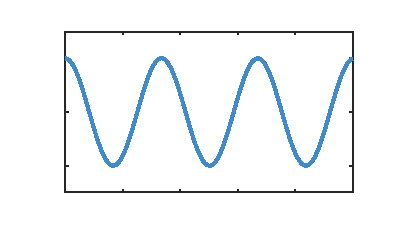
\includegraphics[scale=0.55]{chapter2/freq01_1}
    \end{subfigure}
    \begin{subfigure}{0.38\textwidth}   
        \centering
        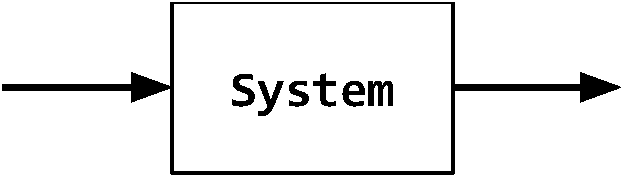
\includegraphics[scale=0.6]{chapter2/freq01_2}
    \end{subfigure}
    \begin{subfigure}{0.25\textwidth}   
        \centering
        $y(t) = M_o cos(\omega t + \phi_o)$\par\medskip
        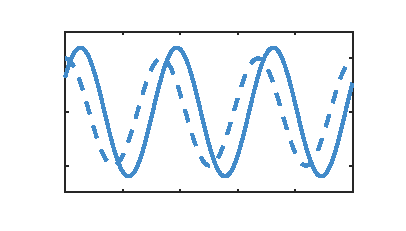
\includegraphics[scale=0.55]{chapter2/freq01_3}
    \end{subfigure}
    
    \caption{Illustration of the steady-state response of LTI systems to sinusoidal inputs.}
    \label{fig:freq01}
\end{figure}

A common representation is the phasor representation, where $M \angle \phi = M cos(\omega t + \phi)$. In the context of SISO Input-Output models, the response of the system can be summarized by a transfer function which is also a phasor:
\begin{equation}
    g(t) = \cfrac{y(t)}{u(t)} = \cfrac{M_o \angle \phi_o}{M_i \angle \phi_i} = M_g \angle \phi_g
,\end{equation}

\noindent where $M_g = M_o / M_i$ and $\phi_g = \phi_o - \phi_i$. Notice that this formulation makes the time-dependance implicit in the system response, since it is periodic in this case. For this reason, the system response can be visualized as a function of frequency rather than a function of time, and the properties of the system can be accessed in this way. The two most popular techniques for frequency response analysis are Bode plots \cite{Bode:1945} and Nyquist diagrams \cite{Nyquist:1932}. The first is a direct plot of $M_g(\omega)$ and $\phi_g(\omega)$ for several values of $\omega$, making $M_g(\omega) = 20 log \left| G(j\omega) \right|$ and $\phi_g(\omega) = \angle G(j\omega)$, where $G(j\omega)$ is a transfer function of a system evaluated for an input signal with exclusively oscillatory components. The Nyquist diagram, in the other hand, is a direct phasor visualization obtained by applying the Argument Principle to a contour containing the entire right-hand side of the complex plane. Both visualizations are depicted in Fig. \ref{fig:freq02}, for a transfer function obtained by applying the transformation of Theorem \ref{th:SSToIO} to the system from \eqref{eq:stateRespEx01}:
\begin{equation} \label{eq:IOSys01}
    \bm{G}(s) = \begin{bmatrix}
        \cfrac{3.81}{s + 5.92} & \cfrac{-1.09s - 3.33}{s^2 + 10.62s + 27.84}
    \end{bmatrix}
.\end{equation}

\begin{figure}[ht] \centering
	\begin{subfigure}{0.46\textwidth}
    	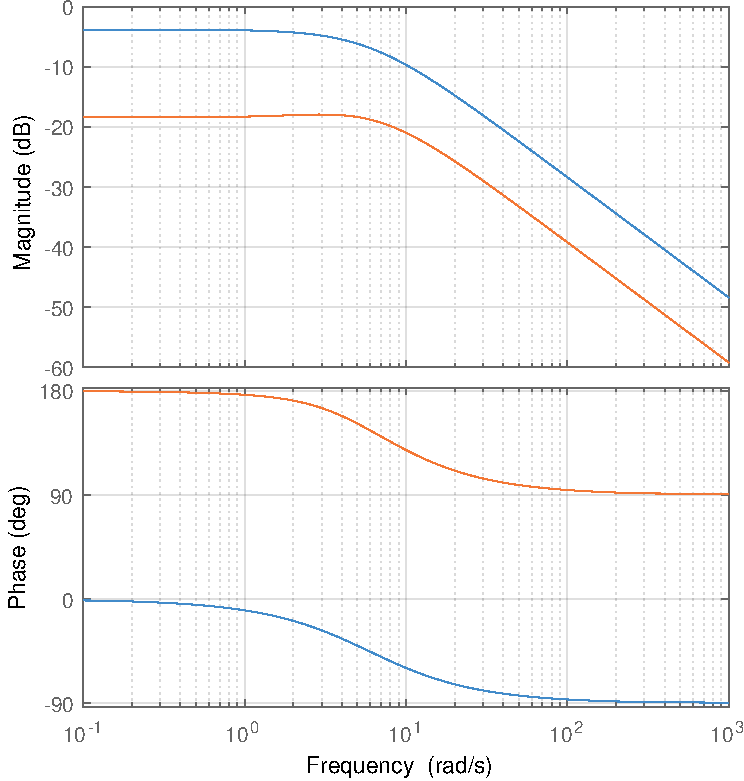
\includegraphics[width=\textwidth]{chapter2/freq02_1}
    \end{subfigure} \hfill
	\begin{subfigure}{0.47\textwidth}
		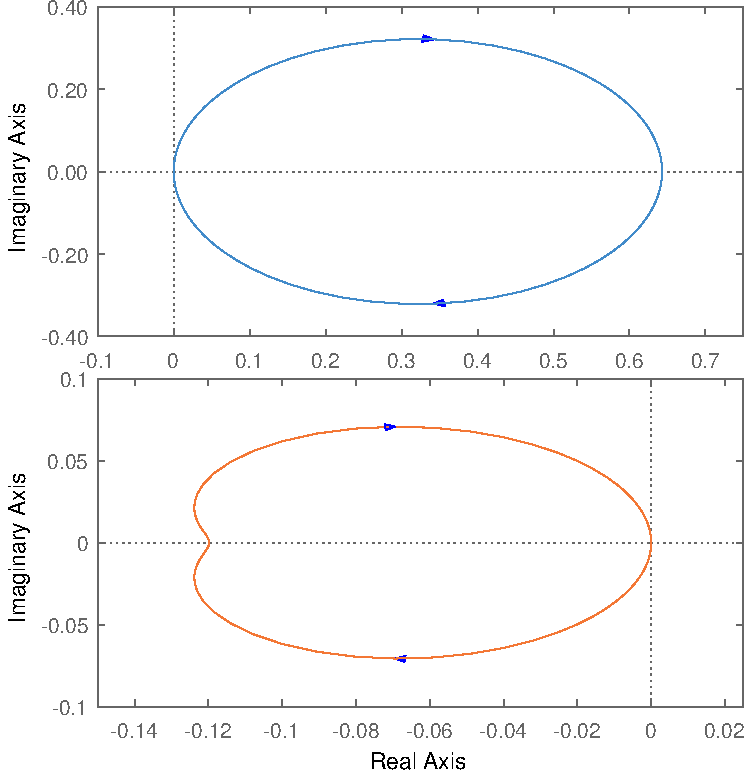
\includegraphics[width=\textwidth]{chapter2/freq02_2}
	\end{subfigure}

    \caption{Visualization of the two-states system in \eqref{eq:IOSys01} in Bode plots (left) and Nyquist diagrams (right). The blue and orange lines represents the states $x_1$ and $x_2$, respectively.}
    \label{fig:freq02}
\end{figure}

The immediate advantage of these visualizations is that is not necessary to compute an entire simulation of this system, until it reaches steady-state, to be able to perform analysis, which is really critic for high-dimensional systems with slow time-constants. In addition to that, these visualizations (specially the Bode plot) can be easily sketched by hand with fairly accuracy, allowing for some understanding of the system without need for solving differential equations or the inverse Laplace transforms. For these reasons, frequency responses methods for analyzing systems were ubiquitous for many years in industry applications, and some properties assessments, such as closed-loop stability, are still better understood under this formulation, as it will be shown in later chapters.

% 3 - Controller Design
% ---------------------------------------------------------------
\clearpage
\chapter{Controller Synthesis}

This chapter discusses the general results and properties for the design of controllers, focusing on feedback architectures. The devices are motivated and formulated using the State-Space model for dynamical systems, so the feedback is performed on the state response rather than on the system output. For this reason, the results in this section focus on this formulation explicitly through the state-equations, where the output-equations are made implicit.

\section{State Feedback Controllers}

In modern control theory, advances in computer performance and the maturing of State-Space model analysis have made the design of controllers using State-Space models feasible for real-world applications. This is usually desirable since these kind of models provides a practical solution to understand dynamical system response and properties, so it is natural to want a controller design technique that accounts for that representation. The most basic, yet very popular, feedback controller used in those settings is the \textit{Full-State Feedback Controller}, defined below. 

\begin{boxed-definition}{Full-State Linear Feedback}
    Given a linear system in State-Space representation, an input action $\bm{u}(t)$ is calculated by the linear control law $\pi(\cdot)$ through state-feedback as:
    \begin{equation}
        \bm{u}(t) = \pi(\bm{r}(t), \bm{x}(t)) = \bm{r}(t) - \bm{K} \bm{x}(t)
    ,\end{equation}
    
    \noindent where $\bm{r} : \mathbb{R} \rightarrow \mathbb{R}^{n}$ is a state reference signal that the system must follows and $\bm{K} \in \mathbb{R}^{r \times n}$ is the \textit{feedback gain matrix}.
\end{boxed-definition}

A block diagram of the closed-loop system for the state-feedback controller is shown at Fig. \ref{fig:feedback01}. In this schematic each blocks represents a function or operation that is applied to the denoted signals, which themselves are represented by the arrows. The direction of the arrows indicates whether the signal variable is an operand or a result of an operation. 

Notice that the control law of the full-state feedback is both linear and time-invariant, which makes the analysis of the closed-loop system similar to the one used in open-loop configurations.  Of course, this is a specific choice of control law, and feedback controllers can also be defined using nonlinear or time-dependent functions. Notice that this new definition for the calculation of $\bm{u}(t)$ allows for the following closed-loop representation of the system:
\begin{align}
\begin{split}
    \dot{\bm{x}}(t) &= \bm{A} \bm{x}(t) + \bm{B} \left( \bm{r}(t) - \bm{K} \bm{x}(t) \right) \\
    	 &= \left( \bm{A} - \bm{B} \bm{K} \right) \bm{x}(t) + \bm{B} \bm{r}(t)
\end{split}
.\end{align}

\begin{figure}[ht]
    \centering
    \resizebox{!}{!}{
    \begin{tikzpicture}[auto, node distance=2cm,>=latex', scale=0.2]
        % We start by placing the blocks
        \node [input, name=input] {};
        \node [sum, right of=input, node distance=4em] (fbckSum) {};
        \node [block, right of=fbckSum] (inputMatrix) {$\bm{B}$};
        \node [sum, right of=inputMatrix, node distance=4em] (stateSum) {};
        \node [block, right of=stateSum, node distance=4em] (integral) {$\int   $};
        \node [block, right of=integral, node distance=8em] (outputMatrix) {$\bm{C}$};
        \node [output, right of=outputMatrix] (output) {};
        \node [block, below of=integral] (stateMatrix) {$\bm{A}$};
        \node [block, below of=stateSum, node distance=10em, label={below:Controller}] (fbckGain) {$\bm{K}$};
        
        \begin{scope}[on background layer]
            \node [fit=(inputMatrix) (stateMatrix) (outputMatrix), fill= myBlue!10, rounded corners, inner sep=.4cm, label={[xshift=3.5em, myBlue!90]above left:Open-Loop System}] {};
        \end{scope}     
        
        % Once the nodes are placed, connecting them is easy.       
        \draw [draw,->] (input) -- node[pos=0.1] {$\bm{r}$} node[pos=0.8] {$+$}  (fbckSum);
        \draw [->] (fbckSum) -- node[pos=0.3]{$\bm{u}$} (inputMatrix);
        \draw [->] (inputMatrix) -- node[pos=0.8]{$+$} (stateSum);
        \draw [->] (stateSum) -- node[pos=0.5]{$\dot{\bm{x}}$} (integral);
        \draw [->] (integral) -- node[name=bk1,pos=0.5]{} node[name=bk2,pos=0.5]{} node[pos=0.5]{$\bm{x}$} (outputMatrix);
        \draw [->] (outputMatrix) -- node[pos=0.6]{$\bm{y}$} (output);
        \draw [->] (bk1) |- (stateMatrix);
        \draw [->] (bk2) |- (fbckGain);
        \draw [->] (stateMatrix) -| node[pos=0.95]{$+$} (stateSum);
        \draw [->] (fbckGain) -| node[pos=0.97]{$-$} (fbckSum);
    \end{tikzpicture} 
    }
    \caption{Block diagram of a state-feedback closed-loop system.}
    \label{fig:feedback01}
\end{figure}

Clearly, the inclusion of a feedback controller in the loop is equivalent to transform an open-loop system into a new system $(\bm{A}_{cl}, \bm{B})$, with $\bm{A}_{cl} = \bm{A} - \bm{B} \bm{K}$, whose manipulated variable is now the reference signal $\bm{r}(t)$. Therefore, an appropriate choice of $\bm{K}$ allows to modify the behavior of the closed-loop system such that a desirable behavior is obtained. To understand better the capabilities of the state feedback, consider the following theorems.

%\begin{boxed-theorem}
%   Given any matrix $\bm{K} \in \mathbb{R}^{r \times n}$, the closed-loop system described by matrices $(\bm{A}-\bm{B}\bm{K}, \bm{B})$ is controllable if and only if the open-loop system $(\bm{A}, \bm{B})$ is controllable.
%\end{boxed-theorem} 
%
%\begin{proof}
%   From definition, the controllability matrix $\bm{\mathcal{C}}_{cl}$ of the closed-loop system is given by:
%   \begin{equation}
%       \bm{\mathcal{C}}_{cl} = \begin{bmatrix} \bm{B} & (\bm{A}-\bm{B}\bm{K})\bm{B} & (\bm{A}-\bm{B}\bm{K})^2 \bm{B} & \cdots & (\bm{A}-\bm{B}\bm{K})^{n-1} \bm{B} \end{bmatrix}
%   \end{equation}
%   
%   It is possible to factorize this matrix as:
%   \begin{equation}
%       \bm{\mathcal{C}}_{cl} = \bm{\mathcal{C}} 
%       \begin{bmatrix} \bm{I} & -\bm{K} \bm{B} & -\bm{K} (\bm{A} - \bm{B}\bm{K})\bm{B} & \cdots & -\bm{K} (\bm{A} - \bm{B}\bm{K})^{n-3}\bm{B} & -\bm{K} (\bm{A} - \bm{B}\bm{K})^{n-2}\bm{B} \\ 
%       0 & \bm{I} & -\bm{K} \bm{B} & \cdots & -\bm{K} (\bm{A} - \bm{B}\bm{K})^{n-4}\bm{B} & -\bm{K} (\bm{A} - \bm{B}\bm{K})^{n-3}\bm{B} \\ 
%       \vdots & \vdots & \vdots & \iddots & \vdots & \vdots \\
%       0 & 0 & 0 & \cdots & -\bm{K} \bm{B} & -\bm{K} (\bm{A} - \bm{B}\bm{K})\bm{B} \\
%       0 & 0 & 0 & \cdots & \bm{I} & -\bm{K} \bm{B} \\
%       0 & 0 & 0 & \cdots & 0 & \bm{I} \end{bmatrix}
%   \end{equation}
%   
%   Notice that the multiplication $\bm{K} \bm{B} \in \mathbb{R}^{1 \times r}$ and $\bm{I} \in \mathbb{R}^{r \times r}$. Since the rightmost matrix is upper-triangular, and has no zeros in the main diagonal, the rank of $\bm{\mathcal{C}}$ and $\bm{\mathcal{C}}_{cl}$ are equal. Therefore, if $\bm{\mathcal{C}}$ has full row rank, so has $\bm{\mathcal{C}}_{cl}$, proving the statement.
%\end{proof}

\begin{boxed-theorem}{(Controller Canonical Form)} \label{th:controlCanon}
    If a SISO system in State-Space representation is controllable, then by applying the transformation $\bm{z}(t) = \bm{P}\bm{x}(t)$, for a matrix $\bm{P}$ calculated as the inverse of:
    \begin{equation}
        \bm{P}^{-1} = \bm{\mathcal{C}} \begin{bmatrix}
        1 & \alpha_1 & \cdots  & \alpha_{n-1} \\
        0 & 1 & \cdots & \alpha_{n-2} \\
        \vdots & \vdots & \ddots & \vdots \\
        0 & 0 & \cdots &1
        \end{bmatrix}
    ,\end{equation}
    
    \noindent where $[\alpha_1, \alpha_2, ..., \alpha_{n-1}]$ are the $n-1$ first coefficients of the characteristic polynomial $\Delta(s) = det(s\bm{I} - \bm{A})$, the resulting representation is in the \textit{controller canonical form} given as:
    \begin{align}
    \begin{cases}
        \dot{\bm{z}}(t) = \begin{bmatrix}
            -\alpha_1 & -\alpha_2 & \cdots & -\alpha_{n-1} & -\alpha_n \\
            1 & 0 & \cdots & 0 & 0 \\
            \vdots & \vdots & \ddots & \vdots & \vdots \\
            0 & 0 & \cdots & 1 & 0 
        \end{bmatrix} \bm{z}(t) + \begin{bmatrix}
            1 \\ 0 \\ \vdots \\ 0
        \end{bmatrix} u(t) \\
        y(t) = \begin{bmatrix} \beta_1 & \beta_2 & \cdots & \beta_n \end{bmatrix} \bm{z}(t)
    \end{cases}
    .\end{align}
\end{boxed-theorem} 

Details for the proof of this theorem can be found in \textbf{[reference]}. An equivalent result can be proved for MIMO systems \textbf{[reference]}, but the result is cumbersome and does not highlight the main results for the state-feedback. Using the canonical form just presented, it is possible to discuss an important result for the state feedback controller.

\begin{boxed-theorem}{(Pole-Placement Method)} \label{th:polePlace}
    If a system in State-Space representation is controllable, then by state feedback using a gain matrix $\bm{K} \in \mathbb{R}^{r \times n}$ the eigenvalues of $\bm{A}_{cl}=\bm{A}-\bm{B}\bm{K}$, the poles of the closed-loop system, can be placed arbitrarily in the complex plane, as long as complex conjugate eigenvalues are assigned in pairs.
\end{boxed-theorem} 

\begin{proof}
    Suppose that the system is controllable. In this case, it can be converted to the controller canonical form of Theorem \ref{th:controlCanon}. Substituting $\bm{z}(t) = \bm{P} \bm{x}(t)$ results in the following control law for the state feedback:
    \begin{equation}
        u(t) = r(t) - \bm{K} \left( \bm{P}^{-1} \bm{z}(t) \right) = r(t) - \tilde{\bm{K}} \bm{z}(t)
    .\end{equation}
    
    \noindent Applying the state feedback, the transformed closed-loop is given by:
    \begin{equation} \label{eq:fdbckContrCanon}
    \tilde{\bm{A}}_{cl} = \bm{P} (\bm{A} - B \bm{K}) \bm{P}^{-1} = \bm{P} \bm{A} \bm{P}^{-1} - \bm{P} B \bm{K} \bm{P}^{-1} = \tilde{\bm{A}} - \tilde{B} \tilde{\bm{K}}
    .\end{equation}   
    
    \noindent From Theorem \ref{th:simTrans01} it is known that $\bm{A}_{cl}$ and $\tilde{\bm{A}}_{cl}$ share the same set of eigenvalues, and, consequently, the same characteristic equations. Consider this characteristic equation as:
    \begin{equation}
        \Delta(s) = det(s\bm{I} - \bm{A}) = s^n + \alpha_1 s^{n-1} + \alpha_2 s^{n-2} + \cdots + \alpha_{n-1} s + \alpha_n
    .\end{equation}
    
    \noindent Given a set of coefficients $[\tilde{\alpha}_1, \tilde{\alpha}_2, ..., \tilde{\alpha}_n]$ for a characteristic polynomial whose roots are the closed-loop eigenvalues, define the transformed feedback gain matrix as:
    \begin{equation}
        \tilde{\bm{K}} = \begin{bmatrix} \tilde{\alpha}_1 - \alpha_1 & \tilde{\alpha}_2 - \alpha_2 & \cdots & \tilde{\alpha}_n - \alpha_n \end{bmatrix}
    .\end{equation}
    
    \noindent Substituting this in \eqref{eq:fdbckContrCanon}, it is easy to see that the resulting representation is:
    \begin{align} \label{eq:SSFdbckControlCanon}
    \begin{cases}
        \dot{\bm{z}}(t) = \begin{bmatrix}
            -\tilde{\alpha}_1 & -\tilde{\alpha}_2 & \cdots & -\tilde{\alpha}_{n-1} & -\tilde{\alpha}_n \\
            1 & 0 & \cdots & 0 & 0 \\
            \vdots & \vdots & \ddots & \vdots & \vdots \\
            0 & 0 & \cdots & 1 & 0 
        \end{bmatrix} \bm{z}(t) + \begin{bmatrix}
            1 \\ 0 \\ \vdots \\ 0
        \end{bmatrix} u(t) \\
        y(t) = \begin{bmatrix} \beta_1 & \beta_2 & \cdots & \beta_n \end{bmatrix} \bm{z}(t)
    \end{cases}
    ,\end{align} 
    
    \noindent whose characteristic polynomial is now described by the designed coefficients that yield the desirable eigenvalues. Since $\tilde{\bm{A}}_{cl}$ and $\bm{A}_{cl}$ shares the same set of eigenvalues, it can be concluded that it is possible to assign the system poles directly through matrix $\tilde{\bm{K}}$.
\end{proof}

Notice that an ``original" feedback gain matrix can be obtained as $\bm{K} = \tilde{\bm{K}} \bm{P}$ and still yield the same eigenvalues assignment directly in $\bm{A}_{cl}$ (since $\bm{P}$ is just a linear transformation). The theorem has the direct result that, under full-state feedback, the transient response of a linear system can be completely determined by including a controller, which is described by this matrix $\bm{K}$. The result is preserved for MIMO systems, although the design of $\bm{K}$ is not as straightforward, since it is not unique for a desired set of eigenvalues in this case \textbf{[reference]}. 

Using the parameters from Definition \ref{def:responseParameters}, the positions of the closed-loop system poles can be designed given desirable operations, and the matrix $\bm{K}$ can be hand-designed to meet these requirements. This method is known as the \textit{Pole-Placement method} for control synthesis. Algorithm \ref{alg:stateFeedback} summarizes a simple procedure of designing an appropriate feedback gain matrix, given desirable pole positions.

\begin{algorithm}[ht] 
    \caption{Pole-Placement Method for SISO Systems} \label{alg:stateFeedback}
    \SetAlgoLined
    \SetKwInOut{Input}{Input}
    \SetKwInOut{Output}{Output}
    
    \Input{State-space model $(\bm{A}, B)$ and a set of $n$ desired eigenvalues $\bm{\lambda}^*$.}
    \Output{Feedback gain matrix $\bm{K}$.}
    \vskip0.25cm
    
    Calculate $[\alpha_1, \alpha_2, ..., \alpha_n]$ as the coefficients of the polynomial $\Delta(s) = det(s\bm{I} - \bm{A})$;
    
    Let $\bm{P}^{-1} = \begin{bmatrix} B & \bm{A} B & \bm{A}^2 B & \cdots & \bm{A}^{n-1} B \end{bmatrix} \begin{bmatrix}
        1 & \alpha_1 & \cdots  & \alpha_{n-1} \\
        0 & 1 & \cdots & \alpha_{n-2} \\
        \vdots & \vdots & \ddots & \vdots \\
        0 & 0 & \cdots &1
        \end{bmatrix}$;
    
    Let $\bm{P} = \left( \bm{P}^{-1} \right)^{-1}$;
    
    Calculate $[\tilde{\alpha}_1, \tilde{\alpha}_2, ..., \tilde{\alpha}_n]$ as the coefficients of the polynomial $\Delta_{cl}(s) = \prod_{i=1}^n (s - \lambda^*_i)$;
    
    Let $\tilde{\bm{K}} = \begin{bmatrix} \alpha_1 - \tilde{\alpha}_1 & \alpha_2 - \tilde{\alpha}_2 & \cdots & \alpha_n - \tilde{\alpha}_n \end{bmatrix}$;
    
    Return $\bm{K} = \tilde{\bm{K}} \bm{P}$;
\end{algorithm} 

Albeit being a simple formula, Pole-Placement can be used in several applications to yield controllers capable of achieve performance requirements. Of course, the designer must take into account that, although the eigenvalue assignment allows for the whole complex plane, a careless choice of eigenvalues could result in controllers requesting very aggressive or oscillatory input signals. For this reason, it is necessary some knowledge of the instruments limits before designing the matrix $\bm{K}$.

\section{Regulation and Reference Tracking}

When discussing controller synthesis it is also necessary to account for the objective that the device is expected to fulfill. There exists two modes of operation that the controller may require for the system: regulation and reference tracking. In the case of state-feedback, these two classes of controllers differs only by what type of reference signal $\bm{r}(t)$, for an operation in a time interval $t \in [t_0, t_f]$, the system is expected to follow. 

\subsubsection{Regulator Problem}

The following statements gives a formal definition of a controller for regulation:

\begin{boxed-definition}{(Regulator)} \label{def:regulator}
    If a state-feedback controller has to make a system follows the reference $\bm{r}(t) = \bm{0}$, as $t \to \infty$, it is said to be a \textit{regulator}. In this case, the closed-loop state equation and equivalent solutions reduces to the following:
        \begin{align}
    \begin{matrix*}[l]
    \textbf{State Equation:} \hfill & & & \textbf{Lagrange solution:} \hfill \\
    \dot{\bm{x}}(t) = \left( \bm{A} - \bm{B} \bm{K} \right) \bm{x}(t)  & & &
    \bm{x}(t) = e^{(\bm{A} - \bm{B} \bm{K}) t} \bm{x}(t_0) \hfill
    \end{matrix*}
    .\end{align}
\end{boxed-definition}

Of course, if the feedback gain matrix impose that all poles of the system are in the left-half plane, the closed-loop is stable and the natural response will eventually converge to zero (Theorem \ref{th:BIBOStab}). Therefore, all stable feedback controllers are able to impose regulation to a system, and the characteristics of the transient response can be fully determined by the matrix $\bm{K}$. These type of controllers are used to make systems goes from nonzero initial states to the zero-state $\bm{x}(t) = \bm{0}$ and stays there, meaning that the the controller can also be used to reject disturbances. Now, one may wonder if this operation is too restrictive in the sense that the zero-state is not the desirable state in many control objectives. However, it is common to have linear systems that are linearized versions of nonlinear models, using the approximation from Theorem \ref{th:linearization}. In these cases, the regulator actually has to impose $\Delta \bm{x}(t) = \bm{x}(t) - \bm{x}_o = \bm{0}$, i.e., drives the system to the steady-state point $\bm{x}_o$ and reject disturbances. 

\begin{boxed-example}{} \label{ex:regulator01}
	For the sake of illustration, considers the first system of \eqref{eq:isoSys02}, repeated here:
	\begin{equation} \label{eq:isoSys02Rep}
	\begin{matrix}
	    \bm{A} = \begin{bmatrix} 
	        -5.93  &      0 \\
	        \hfill 0.83   &  -4.70 
	    \end{bmatrix} &; & b = \begin{bmatrix} 3.81 \\ -1.09 \end{bmatrix}
	\end{matrix}    
	.\end{equation}
	
	\noindent It is easy to verify that this system is controllable, since its controllability matrix is full-rank. In this case, consider the gains $K_1 = [-0.993, 1.221]$, $K_2 = [0.782, 0.549]$ and $K_3 = [0.81, 5.20]$ to yield regulator controllers. The correspondent closed-loop systems $\bm{A}^{(i)}_{cl}$ for each $i$-th controller are given as:
	\begin{equation}
	\begin{matrix}
		\bm{A}^{(1)}_{cl} = \begin{bmatrix} 
	        -2.144 &  -4.651 \\
		   -0.257 & -3.355
	    \end{bmatrix}; & 
	    \bm{A}^{(2)}_{cl} = \begin{bmatrix} 
	        -8.906 & -2.092 \\
    		\phantom{-}1.692 & -4.093
	    \end{bmatrix}; &
	    \bm{A}^{(3)}_{cl} = \begin{bmatrix} 
	        -9.014 & -19.812 \\
    		\phantom{-}1.723 & \phantom{-}1.014
	    \end{bmatrix} &
	\end{matrix}
	.\end{equation}
	
	\noindent Since the open-loop system was obtained by the linearized model in \eqref{eq:isoReact01} for $\bm{x}_o = [6.19, 1.09]^T$ and $u_o = 3.03$, the regulator will impose the zero-state $\Delta \bm{x} = \bm{0}$ which actually means imposing $\bm{x}(t) = [6.19, 1.09]^T$ as $t \to \infty$. 
\end{boxed-example}

The responses of the three closed-loop systems calculated in Example \ref{ex:regulator01} are shown in Fig. \ref{fig:regulator01}. The simulations assumed initial state $\Delta \bm{x}(t) = \bm{0} - \bm{x}_o$, and the response and input signal were vertically corrected by $\bm{x}_o$ and $\bm{u}_o$, respectively. Notice that, as expected, the feedback gains $\bm{K}_i$ can effectively change the system behavior, even causing pseudo-periodic responses.	

\begin{figure}[ht] \centering
    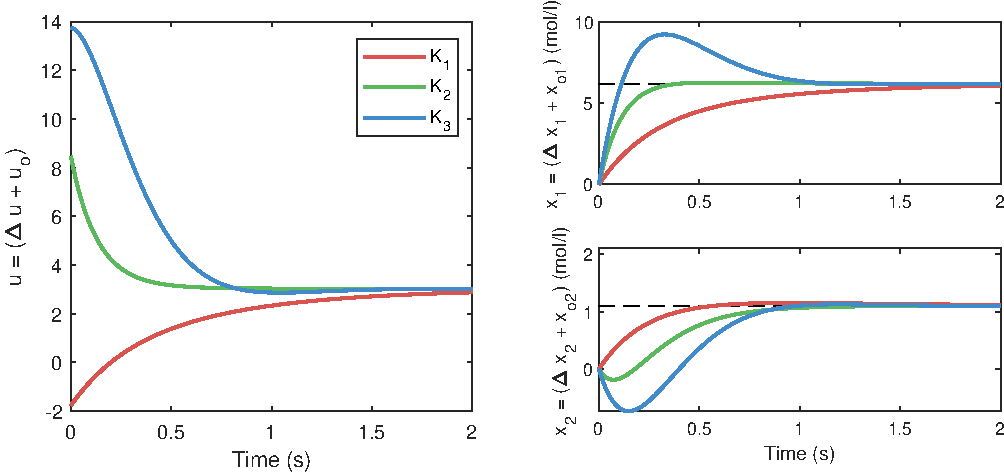
\includegraphics[width=\textwidth]{chapter3/report_ch3_1}
    
    \caption{Simulation of three closed-loop systems from Example \ref{ex:regulator01} showing the input signal (left) and state responses (right).}
    \label{fig:regulator01}
\end{figure}

\subsubsection{Reference Tracking Problem}

In contrast, the control objective could be to follow a non-constant signal $\bm{r}(t)$, or to follow a constant signal different from the zero-state, giving rise to the tracking or servomechanism controllers. A more complete discussion is needed in such cases, since there is a possibility that state-feedback is not capable of actually perform the tracking. To understand this question, consider, for simplicity, that the system must follow a constant reference $\bm{r}(t) = a$. Consider, now, an Input-Output conversion of a closed-loop SISO State-Space model, which from \eqref{eq:SSFdbckControlCanon} directly results in the transfer function:
\begin{equation}
    G(s) = \cfrac{Y(s)}{R(s)} = \cfrac{\beta_1 s^{n-1} + \beta_2 s^{n-2} + \cdots + \beta_{n-1} s + \beta_n}{s^{n} + \tilde{\alpha}_1 s^{n-1} + \tilde{\alpha}_2 s^{n-2} + \cdots + \tilde{\alpha}_{n-1} s + \tilde{\alpha}_n}
.\end{equation}

From that formulation it is clear that the response $Y(s) = G(s)R(s)$ will yield a perfect tracking if $G(s) = 1$. Moreover, if the system has to track asymptotically track this reference, this operation can be evaluated as time $t \to \infty$ or, equivalently, as the frequency $s \to 0$. Plugging this limit in the transfer function implies that a perfect tracking is always possible if $G(0) = \beta_n /  \tilde{\alpha}_n = 1$, which is not guaranteed a priori. A possible solution is to transform the reference with as $\tilde{r}(t) = F r(t)$, so that $Y(s) = G(s)\tilde{R}(s) = G(s) F R(s)$, resulting that:
\begin{equation}
    G(0) F = 1 \Rightarrow F = \cfrac{\tilde{\alpha}_n}{\beta_n}
,\end{equation}

\noindent which allows for perfect asymptotically tracking in all cases but when $\beta_n = 0$. This same reasoning can easily be extended to MIMO systems (the gain $F$ turns into a matrix). In the case of non-constant references, the same intuition could still be used, but the analysis and design of $F$ becomes more complex \textbf{[reference]}. This, however, allows for the definition of tracking controllers.

\begin{boxed-definition}{(Tracking Controllers)} \label{def:tracking}
    If a state-feedback controller has to make a system track any step reference $\bm{r}(t) \neq \bm{0}$, as $t \to \infty$, it is said to be a \textit{tracking controller}. In this case, one has to apply the \textit{feedforward gain} $\bm{F}$ to adapt the reference as $\tilde{\bm{r}}(t) = \bm{F}\bm{r}(t)$, resulting in the following closed-loop state equation and equivalent solution:
    \begin{align}
    \begin{matrix*}[l]
    \textbf{State Equation:} \hfill & & \textbf{Lagrange solution:} \hfill \\
    \dot{\bm{x}}(t) = \left( \bm{A} - \bm{B} \bm{K} \right) \bm{x}(t) + \bm{B} \bm{F} \bm{r}(t)  & &
    \bm{x}(t) = e^{(\bm{A} - \bm{B} \bm{K}) t} \bm{x}(t_0) + \int_{t_0}^{t} e^{(\bm{A} - \bm{B} \bm{K}) (t - \tau)} \bm{B} \bm{F} \bm{r}(\tau) d \tau \hfill
    \end{matrix*}
    .\end{align}
\end{boxed-definition}

Despite being a feasible solution, there are still problems with this definition of tracking controllers. For instance, if the system is subject to a \textit{constant additive disturbance}, which has not been included in the model, the resulting operation will not yield a perfect tracking. 

The problem of the previous formulation for a tracking controller is that it is not robust to actions that happens outside the model. A direct cause of this is the fact that the feedforward gain $\bm{F}$ does not benefit from the real-time corrective action of the state-feedback, but rather is calculated \textit{off-line} using the model properties. Therefore, a way to ensure a more robust operation could be to insert real-time information about the tracking error directly to the feedback corrective action. With this motivation, a new formulation of the tracking controller is given below.

\begin{boxed-definition}{(Robust Tracking Controllers)} \label{def:robustTracking}
    Consider a State-space system and augmented state $\bm{x}_a : \mathbb{R} \rightarrow \mathbb{R}^{p}$ defined by:
    \begin{equation}
        \bm{x}_a(t) = \int_{0}^{t} \bm{r}(\tau) - \bm{y}(\tau) d\tau \Longrightarrow \dot{\bm{x}}_a(t) = \bm{r}(t) - \bm{y}(t)
    .\end{equation}
    
\noindent A robust tracking (or servo) controller, defined by the gain $\tilde{\bm{K}} = \begin{bmatrix} \bm{K} & \bm{K}_a \end{bmatrix}$, for $\bm{K} \in \mathbb{R}^{r \times n}$ and $\bm{K}_a \in \mathbb{R}^{r \times p}$, operates on the following augmented version of the original system:
    \begin{align} \label{eq:augmentedSystem}
    \begin{cases}
        \begin{bmatrix}
            \dot{\bm{x}}(t) \\
            \dot{\bm{x}}_a(t)
        \end{bmatrix} &= \begin{bmatrix}
            \bm{A} - \bm{B} \bm{K} & -\bm{B} \bm{K}_a \\ - \bm{C} & \bm{0}
        \end{bmatrix} \begin{bmatrix}
            \bm{x}(t) \\
            \bm{x}_a(t)
        \end{bmatrix} + \begin{bmatrix}
            \bm{0} \\
            \bm{I_p}
        \end{bmatrix} \bm{r}(t)
        \\
        \hfill \bm{y}(t) &= \begin{bmatrix}
            \bm{C} & \bm{0}
        \end{bmatrix} \begin{bmatrix}
            \bm{x}(t) \\
            \bm{x}_a(t)
        \end{bmatrix}
    \end{cases}
    \end{align}
    
    \noindent or, equivalently:
    \begin{align}
    \begin{cases}
        \dot{\tilde{\bm{x}}}(t) = \tilde{\bm{A}}_{cl} \tilde{\bm{x}}(t) + \tilde{\bm{B}} \bm{r}(t) \\
        \bm{y}(t) = \tilde{\bm{C}} \tilde{\bm{x}}(t) \hfill
    \end{cases}
    .\end{align}
\end{boxed-definition}

Since the augmented state $\bm{x}_a(t)$ represents an integral of the tracking error until a time $t$, this formulation is usually characterized as imposing ``integral action" to the controller. The schematic in Fig. \ref{fig:tracking02} illustrates how an integrator can be included to the block diagram of the control loop.

\begin{figure}[ht]
    \centering
    \resizebox{\textwidth}{!}{
    \begin{tikzpicture}[auto, node distance=2cm,>=latex']
        % We start by placing the blocks
        \node [input, name=input] {};
        \node [sum, right of=input, node distance=4em] (intFbckSum) {};
        \node [block, right of=intFbckSum, node distance=4em] (integralAction) {$\int$};
        \node [block, right of=integralAction, node distance=6em] (intActGain) {$\bm{K}_a$};
        \node [sum, right of=intActGain, node distance=4.5em] (fbckSum) {};
        \node [block, right of=fbckSum] (inputMatrix) {$\bm{B}$};
        \node [sum, right of=inputMatrix, node distance=4em] (stateSum) {};
        \node [block, right of=stateSum, node distance=4em] (integral) {$\int   $};
        \node [block, right of=integral, node distance=8em] (outputMatrix) {$\bm{C}$};
        \node [output, right of=outputMatrix] (output) {};
        \node [block, below of=integral] (stateMatrix) {$\bm{A}$};
        \node [block, below of=stateSum, node distance=10em, label={below:Controller}] (fbckGain) {$\bm{K}$};
        
        \begin{scope}[on background layer]
            \node [fit=(inputMatrix) (stateMatrix) (outputMatrix), fill= myBlue!10, rounded corners, inner sep=.4cm, label={[xshift=3.5em, myBlue!90]above left:Open-Loop System}] {};
        \end{scope}     
        
        \begin{scope}[on background layer]
            \node [fit=(integralAction) (intActGain), fill= myGreen!10, rounded corners, inner sep=.4cm, label={[xshift=4.3em, myGreen!90]above left:Integral Action}] {};
        \end{scope} 
        
        % Once the nodes are placed, connecting them is easy.       
        \draw [draw,->] (input) -- node[pos=0.1] {$\bm{r}$} node[pos=0.8] {$+$}  (intFbckSum);
        \draw [->] (intFbckSum) -- (integralAction);
        \draw [->] (integralAction) -- node[pos=0.5]{$\bm{x}_a$} (intActGain);
        \draw [->] (intActGain) -- node[pos=0.8]{$-$} (fbckSum);
        \draw [->] (fbckSum) -- node[pos=0.3]{$\bm{u}$} (inputMatrix);
        \draw [->] (inputMatrix) -- node[pos=0.8]{$+$} (stateSum);
        \draw [->] (stateSum) -- node[pos=0.5]{$\dot{\bm{x}}$} (integral);
        \draw [->] (integral) -- node[name=bk1,pos=0.5]{} node[name=bk2,pos=0.5]{} node[pos=0.5]{$\bm{x}$} (outputMatrix);
        \draw [->] (outputMatrix) -- node[name=bk3,pos=0.5]{} node[pos=0.6]{$\bm{y}$} (output);
        \draw [->] (bk1) |- (stateMatrix);
        \draw [->] (bk2) |- (fbckGain);
        \draw [->] (stateMatrix) -| node[pos=0.95]{$+$} (stateSum);
        \draw [->] (fbckGain) -| node[pos=0.97]{$-$} (fbckSum);
        \draw [->] (bk3) -- ++(0, -14em) -| node[pos=0.97]{$-$} (intFbckSum);
    \end{tikzpicture} 
    }
    \caption{Block diagram of a state-feedback closed-loop system with integral action.}
    \label{fig:tracking02}
\end{figure}

Notice that state-equation for closed-loop of this new augmented system is resulting from
\begin{equation}  \label{eq:augmentedSystem02} 
	\tilde{\bm{A}}_{cl} = \begin{bmatrix} \phantom{-}\bm{A} & \bm{0} \\ -\bm{C} & \bm{0} \end{bmatrix} - \begin{bmatrix} \bm{B} \bm{K} & \bm{B} \bm{K}_a \\ \bm{0} & \bm{0} \end{bmatrix} = \begin{bmatrix} \phantom{-}\bm{A} & \bm{0} \\ -\bm{C} & \bm{0} \end{bmatrix} - \begin{bmatrix} \bm{B} \\ \bm{0} \end{bmatrix} \begin{bmatrix} \bm{K} & \bm{K}_a \end{bmatrix} = \tilde{\bm{A}} - \tilde{\bm{B}} \tilde{\bm{K}}
.\end{equation}

\noindent In this case, it must be discussed whether the new gain $\tilde{\bm{K}}$ still preserves the eigenvalue assignment property of a state-feedback gain defined on the original State-Space model.

\begin{boxed-theorem}{} \label{th:augmentedCtrb}
    If the SISO system described by $(\bm{A}, B)$ is controllable and its transfer function $G(s)$ has no zero at $s = 0$, then the eigenvalues of the augmented matrix $\tilde{\bm{A}}$ can be assigned arbitrary by the feedback gain $\tilde{\bm{K}}$.
\end{boxed-theorem}

\begin{proof}
    Consider a SISO controllable system. After the augmentation, the new controllability matrix $\tilde{\bm{\mathcal{C}}} \in \mathbb{R}^{(n+p)\times nr}$ is calculated as:
    \begin{align}
    \begin{split}
        \tilde{\bm{\mathcal{C}}} &= \begin{bmatrix}
        \begin{array}{c c c c c c}
            B & \bm{A} B & \bm{A}^2 B & \bm{A}^3 B & \cdots & \bm{A}^{n-1} B \\ 
            0 & -C B & -C \bm{A} B & -C \bm{A}^2 B & \cdots & -C \bm{A}^{n-2} B
        \end{array}
        \end{bmatrix} \\
        &=
            \begin{bmatrix}
            \begin{array}{c c c c c c}
                1 & -\alpha_1 & -\alpha_1^2 - \alpha_2 & -\alpha_1(\alpha_1^2 - \alpha_2) + \alpha_2 \alpha_1 - \alpha_3 & \cdots & \Delta_1(\alpha_1,...,\alpha_n) \\
                0 & 1 & -\alpha_1 & -\alpha_1^2 - \alpha_2  & \cdots & \Delta_2(\alpha_1,...,\alpha_n) \\
                0 & 0 & 1 & -\alpha_1  & \cdots & \Delta_1(\alpha_1,...,\alpha_n) \\
                0 & 0 & 0 & 1 &  \cdots & \Delta_3(\alpha_1,...,\alpha_n) \\
                \vdots & \vdots & \vdots & \vdots & \ddots & \vdots \\
                0 & 0 & 0 & 0 & \cdots & \Delta_{n}(\alpha_1,...,\alpha_n) \\
                0 & -\beta_1 & -\beta_1 \alpha_1 - \beta_2 & -\beta_1(\alpha_1^2 - \alpha_2) + \beta_2 \alpha_1 - \beta_3  & \cdots & \Delta_{n+1}(\alpha_1,...,\alpha_n)
            \end{array}
            \end{bmatrix},
    \end{split}
    \end{align}
    
    \noindent where $\Delta_i(\alpha_1,...,\alpha_n)$ is a polynomial used to save space in the equations. By inspection of this matrix, it is possible to discover a pattern between the rows. Since elementary operations between the rows ${r_1, r_2, ..., r_n}$ do not change the matrix row rank, the last row of the matrix can be transformed as $r_n = r_n + r_{n-1}\beta_{n-2} + r_{n-2}\beta_{n-3} + \cdots + r_{2}\beta_{1}$. The result is the triangular matrix in the form:
    \begin{align}
    \begin{split}
        \tilde{\bm{\mathcal{C}}} &= 
            \begin{bmatrix}
                1 & -\alpha_1 & -\alpha_1^2 - \alpha_2 & -\alpha_1(\alpha_1^2 - \alpha_2) + \alpha_2 \alpha_1 - \alpha_3 & \cdots & \Delta_1(\alpha_1,...,\alpha_n) \\
                0 & 1 & -\alpha_1 & -\alpha_1^2 - \alpha_2  & \cdots & \Delta_2(\alpha_1,...,\alpha_n) \\
                0 & 0 & 1 & -\alpha_1  & \cdots & \Delta_3(\alpha_1,...,\alpha_n) \\
                0 & 0 & 0 & 1 &  \cdots & \Delta_4(\alpha_1,...,\alpha_n) \\
                \vdots & \vdots & \vdots & \vdots & \ddots & \vdots \\
                0 & 0 & 0 & 0 & \cdots & \Delta_{n}(\alpha_1,...,\alpha_n) \\
                0 & 0 & 0 & 0  & \cdots & \beta_n
            \end{bmatrix}
    \end{split}
    .\end{align}
    
    Since $G(s)$ has no zeros at $s = 0$, then $\beta_n \neq 0$, meaning that $\tilde{\bm{\mathcal{C}}}$ is nonsingular and, therefore has full row rank. From this it can be concluded that the augmented system $(\tilde{\bm{A}}, \tilde{B})$ is controllable and, from Theorem \ref{th:polePlace}, the eigenvalues of $\tilde{\bm{A}}$ can be assigned anywhere in the complex plane.
\end{proof}

Although the result was only shown for the SISO case, the main intuition still holds in the MIMO case, but the equations become cumbersome. Basically, if the augmented matrices are controllable, the robust tracking can be achieved by the same formulation. 

A possible intuition on how this system performs robust tracking and disturbance rejection can be taken from the fact that the first row of \eqref{eq:augmentedSystem02} has the same form of a basic regulator, except from the term $\bm{B} \bm{K}_a$ which is a linear function of $\bm{x}_a(t)$. Because of this, a control action will always be requested whenever $\bm{x}_a(t) \neq \bm{0}$, i.e., when there is an error between the reference and the output signal. When $\bm{x}_a(t) = \bm{0}$, the equation reduces to a simple regulator. A more quantitative analysis on why this controller yields both robust tracking and disturbance rejection can be found in \textbf{[reference]}. 

\begin{boxed-example}{}
	For the sake of illustration, consider the same system used in \eqref{eq:isoSys02Rep}. Unfortunately, the augmented version of this \textit{single-input multiple-output} (SIMO) formulation is not controllable. However, the SISO version obtained by letting $C = \begin{bmatrix} 0, 1 \end{bmatrix}$ obeys Theorem \ref{th:augmentedCtrb} and has no zeros at $s=0$. Thus, a robust tracking controller can be designed by state-feedback. Consider the gains $\tilde{K}_1 = [-0.99, 1.22, -25]$, $\tilde{K}_2 = [0.78, 0.55, -25]$ and $\tilde{K}_3 = [0.81, 5.20, -50]$. The correspondent closed-loop systems $tilde{\bm{A}}^{(i)}_{cl}$ for each $i$-th controller are given as:
	\begin{equation}
	\begin{matrix}
		\tilde{\bm{A}}^{(1)}_{cl} = \begin{bmatrix*}[r] 
	       -9.70 7 & \phantom{-}4.65 & -95.25 \\
    \phantom{-}1.92 & -6.04 & \phantom{-}27.45 \\
         0 & -1.00     &   0
	    \end{bmatrix*}; & \tilde{B} = \begin{bmatrix} 0 \\ 0 \\ 1 \end{bmatrix} \\ \\
	    \tilde{\bm{A}}^{(2)}_{cl} = \begin{bmatrix*}[r] 
	        -2.94 &  2.09 & -95.25 \\
   			-0.02 & -5.30 &  27.46 \\
         		  0 & -1.00  &      0
	    \end{bmatrix*}; & \tilde{B} = \begin{bmatrix} 0 \\ 0 \\ 1 \end{bmatrix} \\ \\
	    \tilde{\bm{A}}^{(3)}_{cl} = \begin{bmatrix*}[r] 
	        -2.84 & 19.81 &-190.50 \\
	 	  	-0.06 & -10.41 & 54.91 \\
        		 0  & -1.00   &     0
	    \end{bmatrix*}; & \tilde{B} = \begin{bmatrix} 0 \\ 0 \\ 1 \end{bmatrix}
	\end{matrix}.
	\end{equation}
\end{boxed-example}

Some simulations of closed-loop systems for this system to track are shown in Fig. \ref{fig:tracking03} for a non-constant reference consisting of a sequence of step signals.

\begin{figure}[ht] \centering
    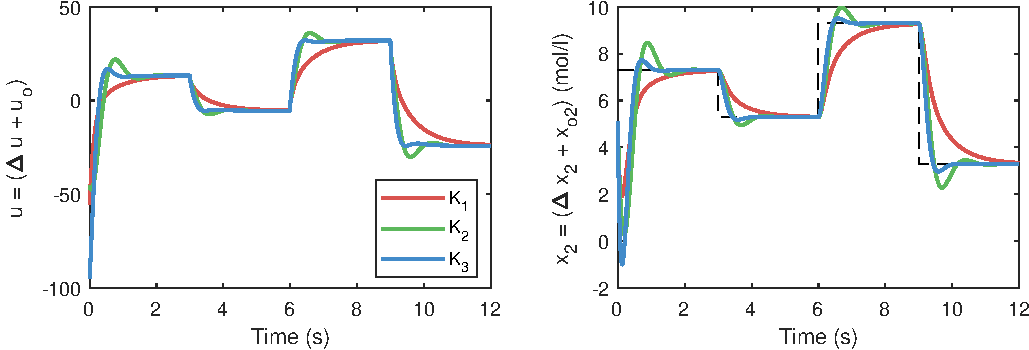
\includegraphics[width=\textwidth]{chapter3/report_ch3_2}
    
    \caption{Simulation of three closed-loop systems showing the input signal (left) and state response (right) for reference tracking. The reference signal is indicated by the black dashed line.}
    \label{fig:tracking03}
\end{figure}


\section{Deterministic State Observers}

Until now, the state feedback was discussed from the perspective that the device has direct access to the real value of all the states of the system. This assumption is unrealistic, since the states are only observed through the output signal $\bm{y}(t)$, through the matrix $\bm{C}$, which itself is not assumed to be always equal to the identity matrix. In practice, this means that some states could not be measured, due to technical difficulties or economic reasons, or that the instrumentation available is not perfect, and the observations are prone to deviate from the real value. Since the state-vector is necessary for the state-feedback to compute the input to the system, this section discusses how to develop devices that can reconstruct the states from the observations.

A device that determines a state-vector $\bm{x}(t)$ from the output signal $\bm{y}(t)$ is known as \textit{state observer}, or \textit{state estimator} in some cases. Amongst several possible techniques, a practical and popular one is the \textit{Luenberger observer}, which is defined below.

\begin{boxed-definition}{(Luenberger Observer)} \label{def:luenberger}
    Given a system in State-Space with output signal $\bm{y}(t) : \mathbb{R} \rightarrow \mathbb{R}^p$ and an observer gain $\bm{L} \in \mathbb{R}^{n \times p}$, the estimated state-vector $\hat{\bm{x}}(t)$ is represented by the observer system:
    \begin{equation}
        \dot{\hat{\bm{x}}}(t) = \bm{A} \hat{\bm{x}}(t) + \bm{B} \bm{u}(t) + \bm{L} \left( \bm{y}(t) - \bm{C} \hat{\bm{x}}(t) \right)
    ,\end{equation}
    
    \noindent or, equivalently:
    \begin{equation} \label{eq:luenberger02}
        \dot{\hat{\bm{x}}}(t) = \left( \bm{A} - \bm{L} \bm{C} \right) \hat{\bm{x}}(t) + \bm{B} \bm{u}(t) + \bm{L} \bm{y}(t)
    .\end{equation}
\end{boxed-definition}

The observer system works as a parallel system that is simulated alongside the actual system, as illustrate in Fig. \ref{fig:luenberger01}. The expected result is that the observer yields $\hat{\bm{x}}(t) = \bm{x}(t)$, as time $t \to \infty$. Alternatively, it is possible to create a variable $\bm{e}(t) = \bm{x}(t) - \hat{\bm{x}}(t)$ such that, using \eqref{eq:luenberger02}:
\begin{align}
\begin{split}
    \dot{\bm{e}} &= \bm{x} - \hat{\bm{x}} \\ 
        &= \left( \bm{A} \bm{x} + \bm{B} \bm{u} \right) - \left( \left( \bm{A} - \bm{L} \bm{C} \right) \hat{\bm{x}} + \bm{B} \bm{u} + \bm{L} \bm{C} \bm{x} \right) \\
        &= \left( \bm{A} - \bm{L} \bm{C} \right) \bm{x} - \left( \bm{A} - \bm{L} \bm{C} \right) \hat{\bm{x}} \\
        &= \left( \bm{A} - \bm{L} \bm{C} \right) \left( \bm{x} - \hat{\bm{x}} \right) \\
        &= \left( \bm{A} - \bm{L} \bm{C} \right) \bm{e}
\end{split}
,\end{align}

\noindent which implies that the observer asymptotically tracks the actual state-vector if $\bm{e}(t) = \bm{0}$ as $t \to \infty$. Analyzing the equation above, it is intuitive to notice that this result can be guaranteed if all the eigenvalues of matrix $\bm{A}_{obs} = \bm{A} - \bm{L} \bm{C}$ have negative real parts, since it implies that the natural response of $\dot{\bm{e}}$ vanishes and there is no forcing input action to yield forcing response to this variable (Theorem \ref{th:BIBOStab}). Therefore, a specific gain $\bm{L}$ could be designed to ensure this condition and allows the observer to asymptotically track the state-vector with a desired behavior. The following theorem relates this statement with the choice of a gain $\bm{L}$.

\begin{figure}[ht]
    \centering
    \resizebox{!}{!}{
    \begin{tikzpicture}[auto, node distance=2cm,>=latex']
        % We start by placing the blocks
        \node [input](input) {};
        \node [block, right of=input, minimum height=4em, node distance=18em, fill=myBlue!20] (openLoopSystem) {Open-Loop System};
        \node [output, right of=openLoopSystem, node distance=18em] (output) {};

        \node [block, below of=openLoopSystem, node distance=6em] (integralLU) {$\int   $};     
        \node [sum, left of=integralLU, node distance=4em] (stateSumLU1) {};                
        \node [sum, left of=stateSumLU1, node distance=3em] (stateSumLU2) {};       
        \node [block, left of=stateSumLU2, node distance=4em] (inputMatrixLU) {$\bm{B}$};
        \node [block, right of=integralLU, node distance=8em] (outputMatrixLU) {$\bm{C}$};
        \node [block, below of=integralLU] (stateMatrixLU) {$\bm{A}$};
        \node [block, below of=stateMatrixLU] (luenbergerGain) {$\bm{L}$};      
        \node [sum, right of=outputMatrixLU, node distance=4em] (fbckOutput) {};    
        
        \begin{scope}[on background layer]
            \node [fit=(inputMatrixLU) (luenbergerGain) (fbckOutput), fill= myRed!10, rounded corners, inner sep=.4cm, label={[xshift=-4em, myRed!90]below right:Luenberger Observer}] {};
        \end{scope} 
        
        % Once the nodes are placed, connecting them is easy.       
        \draw [draw,->] (input) -- node[pos=0.1]{$\bm{u}$} node[name=bk1,pos=0.25]{} (openLoopSystem);
        \draw [->] (openLoopSystem) -- node[name=bk2,pos=0.75]{} node[pos=0.9]{$\bm{y}$}  (output);
        
        \draw [->] (bk1) |-  (inputMatrixLU);
        \draw [->] (bk2) |- node[pos=0.8]{$+$}  (fbckOutput);
        
        \draw [->] (inputMatrixLU) -- node[pos=0.8]{$+$} (stateSumLU2);
        \draw [->] (stateSumLU2) -- node[pos=0.8]{$+$} (stateSumLU1);
        \draw [->] (stateSumLU1) -- node[pos=0.5]{$\dot{\hat{\bm{x}}}$} (integralLU);
        \draw [->] (integralLU) -- node[name=bk1,pos=0.5]{} node[pos=0.5]{$\hat{\bm{x}}$} (outputMatrixLU);
        \draw [->] (outputMatrixLU) -- node[pos=0.8]{$-$} (fbckOutput);
        \draw [->] (bk1) |- (stateMatrixLU);
        \draw [->] (fbckOutput) |- (luenbergerGain);
        \draw [->] (stateMatrixLU) -| node[pos=0.95]{$+$} (stateSumLU1);
        \draw [->] (luenbergerGain) -| node[pos=0.95]{$+$} (stateSumLU2);
    \end{tikzpicture} 
    }
    \caption{Block diagram of a State-Space system with Luenberger observer.}
    \label{fig:luenberger01}
\end{figure}

\begin{boxed-theorem}
    If a system in State-Space representation is observable, then by a Luenberger observer with gain matrix $\bm{L} \in \mathbb{R}^{n \times p}$ the eigenvalues of $\bm{A}_{obs} = \bm{A} - \bm{L} \bm{C}$ can arbitrarily be assigned anywhere in the complex plane, as long as that complex conjugate eigenvalues are assigned in pairs.
\end{boxed-theorem} 

\begin{proof}
    Consider that a State-Space with matrices $(\bm{A}, \bm{C})$ is observable. From the Duality Theorem \textbf{[reference]} if the pair $(\bm{A}, \bm{C})$ is observable then the pair $(\bm{A}^T, \bm{C}^T)$ is controllable. In this case, it is possible to design     a gain matrix $\bm{K}$ to assign the eigenvalues of $\tilde{\bm{A}}_{obs} = \bm{A}^T - \bm{C}^T \bm{K}$ in any desirable points in the complex space. Since the eigenvalues of a matrix are invariant to the transpose operation, the design of $\bm{K}$ can also place the eigenvalues of the matrix $(\tilde{\bm{A}}_{obs})^T = \bm{A} - \bm{K}^T \bm{C}$. Therefore, making $\bm{L} = \bm{K}^T$ proves the theorem.
\end{proof}

The procedure stated in this proof highlights the similarities between existing closed-loop observers, such as the Luenberger observer, and closed-loop controllers, such as the state-feedback. Basically, the same design considerations that concerns state-feedback are important in the design of the observer gain $\bm{L}$. For instance, the eigenvalues of $\tilde{\bm{A}}_{obs} = \bm{A}^T - \bm{C}^T \bm{K}$ can be assigned such that the time evolution of the error $\bm{e}(t)$ has a desirable time constant, damping coefficient or natural frequency. In conclusion, the state-vector $\bm{x}(t)$ can be reconstructed by using an observer gain such that each eigenvalue of $\bm{A}_{obs}$ is on the left-half side of the complex plane. 

The only reason to develop an observer is to allow for state-feedback controllers to access the values of the state-vector, thus being able to calculate an appropriate action to follow the reference signal. If a controller can only access the estimated state-vector $\tilde{\bm{x}}(t)$, it is possible to define a State-Space formulation for a closed-loop based on feedback from estimated states given data from a, possibly non-linear and time-varying, disturbed system.

\begin{boxed-definition}{(Feedback from Estimated States)} \label{def:fdbckLuenberger}
    Given a system in State-Space representation whose state-vector is reconstructed from a Luenberger observer of gain $\bm{L} \in \mathbb{R}^{n \times p}$ and input signal is calculated through state-feedback with gain $\bm{K} \in \mathbb{R}^{n \times r}$, its time evolution can be represented through the model:
    \begin{align} \label{eq:fdbckLuenberger01}
    \begin{cases}
        \dot{\bm{x}}(t) = \bm{A} \bm{x}(t) - \bm{B} \bm{K} \hat{\bm{x}}(t) + \bm{B} \bm{r}(t) \\
        \dot{\hat{\bm{x}}}(t) = \left(\bm{A} - \bm{L} \bm{C} - \bm{B} \bm{K} \right) \hat{\bm{x}}(t) + \bm{B} \bm{r}(t) + \bm{L} \bm{C} \bm{x}(t) 
    \end{cases}
    .\end{align}
\end{boxed-definition} 

A schematic for this formulation of feedback from estimated states is shown Fig. \ref{fig:observer02}, including the possibility for integral action. In fact, this schematic summarizes several different control architectures that includes both feedback action and state estimation, and it will be a reference whenever this work mentions physical control loops and instrumentation.

\begin{figure}[ht]
    \centering
    \resizebox{\textwidth}{!}{
    \begin{tikzpicture}[auto, node distance=2cm,>=latex']
        % We start by placing the blocks
        \node [input, name=input] {};
        \node [sum, right of=input, node distance=3em] (intFbckSum) {};
        \node [block, right of=intFbckSum, node distance=4em] (integralAction) {$\int$};
        \node [block, right of=integralAction, node distance=6em] (intActGain) {$\bm{K}_a$};
        \node [sum, right of=intActGain, node distance=4.5em] (fbckSum) {};
        \node [block, right of=fbckSum, node distance=6em] (inputMatrix) {$\bm{B}$};
        \node [sum, right of=inputMatrix, node distance=4em] (stateSum) {};
        \node [block, right of=stateSum, node distance=4em] (integral) {$\int   $};
        \node [block, right of=integral, node distance=8em] (outputMatrix) {$\bm{C}$};
        \node [output, right of=outputMatrix, node distance=7em] (output) {};
        \node [block, below of=integral] (stateMatrix) {$\bm{A}$};
        
        \node [block, below of=stateMatrix, node distance=12.5em] (integralLU) {$\int$};        
        \node [sum, left of=integralLU, node distance=4em] (stateSumLU) {};             
        \node [block, left of=stateSumLU, node distance=4em] (inputMatrixLU) {$\bm{B}$};
        \node [block, right of=integralLU, node distance=8em] (outputMatrixLU) {$\bm{C}$};
        \node [block, below of=integralLU] (stateMatrixLU) {$\bm{A}$};
        \node [block, above of=integralLU] (luenbergerGain) {$\bm{L}$};     
        
        \draw [->] (outputMatrix) -- node[name=bk3,pos=0.33]{} node[name=bk5,pos=0.8]{} node[pos=0.9]{$\bm{y}$} (output);
        \node [sum, anchor=base] (fbckOutput) at (bk3.base |- luenbergerGain) {};
        
        \node [block, below of=stateSumLU, node distance=11em, label={below:Controller}] (fbckGain) {$\bm{K}$};     
        
        \begin{scope}[on background layer]
            \node [fit=(inputMatrix) (stateMatrix) (outputMatrix), fill= myBlue!10, rounded corners, inner sep=.4cm, label={[xshift=3.5em, myBlue!90]above left:Open-Loop System}] {};
        \end{scope}     
        
        \begin{scope}[on background layer]
            \node [fit=(integralAction) (intActGain), fill= myGreen!10, rounded corners, inner sep=.4cm, label={[xshift=4.3em, myGreen!90]above left:Integral Action}] {};
        \end{scope} 
        
        \begin{scope}[on background layer]
            \node [fit=(inputMatrixLU) (luenbergerGain) (stateMatrixLU) (fbckOutput), fill= myRed!10, rounded corners, inner sep=.4cm, label={[xshift=5.8em, myRed!90]above left:Luenberger Observer}] {};
        \end{scope} 
        
        % Once the nodes are placed, connecting them is easy.       
        \draw [draw,->] (input) -- node[pos=0.1] {$\bm{r}$} node[pos=0.8] {$+$}  (intFbckSum);
        \draw [->] (intFbckSum) -- (integralAction);
        \draw [->] (integralAction) -- node[pos=0.5]{$\bm{x}_a$} (intActGain);
        \draw [->] (intActGain) -- node[pos=0.8]{$-$} (fbckSum);
        \draw [->] (fbckSum) -- node[pos=0.3]{$\bm{u}$} node[name=bku1, pos=0.5]{} (inputMatrix);
        \draw [->] (inputMatrix) -- node[pos=0.8]{$+$} (stateSum);
        \draw [->] (stateSum) -- node[pos=0.5]{$\dot{\bm{x}}$} (integral);
        \draw [->] (integral) -- node[name=bk1,pos=0.5]{} node[name=bk2,pos=0.5]{} node[pos=0.5]{$\bm{x}$} (outputMatrix);
        \draw [->] (bk1) |- (stateMatrix);
        \draw [->] (stateMatrix) -| node[pos=0.95]{$+$} (stateSum);
        \draw [->] (fbckGain) -| node[pos=0.98]{$-$} (fbckSum);
        \draw [->] (bk5) |- ++(0, -33em) -| node[pos=0.98]{$-$} (intFbckSum);
        
        
        \draw [->] (bku1) |- (inputMatrixLU);
        \draw [->] (inputMatrixLU) -- node[pos=0.8]{$+$} (stateSumLU);
        \draw [->] (stateSumLU) -- node[pos=0.5]{$\dot{\hat{\bm{x}}}$} (integralLU);
        \draw [->] (integralLU) -- node[name=bk4,pos=0.5]{} node[pos=0.5]{$\hat{\bm{x}}$} (outputMatrixLU);
        \draw [->] (outputMatrixLU) -| node[pos=0.95]{$-$} (fbckOutput);
        \draw [->] (bk4) |- (stateMatrixLU);
        \draw [->] (fbckOutput) -- (luenbergerGain);
        \draw [->] (stateMatrixLU) -| node[pos=0.95]{$+$} (stateSumLU);
        \draw [->] (luenbergerGain) -| node[pos=0.95]{$+$} (stateSumLU);
        \draw [->] (bk3) -- node[pos=0.95]{$+$} (fbckOutput);
        
        \draw [->] (bk4) |- (fbckGain);
    \end{tikzpicture} 
    }
    \caption{Block diagram of a state-feedback closed-loop system with integral action and Luenberger observer.}
    \label{fig:observer02}
\end{figure}

Notice, now, that the formulation just defined imposes that the dynamics of the estimated state $\hat{\bm{x}}(t)$ is dependent both in $\bm{K}$ and $\bm{L}$, which are arbitrary matrices chosen by the control designer. This leads to the possible conclusion that the choice of $\bm{K}$ is now restricted by the effect that it will produce in the choice of $\bm{L}$, which is not true. The following theorem, known as the Separation Principle \textbf{[reference]}, states that design of these two gains are independent.

\begin{boxed-theorem}{(Separation Principle)} \label{th:separationPrinciple}
    Given a system in State-Space with a Luenberger observer of gain $\bm{L}$ and state-feedback controller of gain $\bm{K}$, the closed-loop eigenvalues contributions of $(\bm{A} - \bm{B}\bm{K})$ are independent from those of $(\bm{A} - \bm{L}\bm{C})$.
\end{boxed-theorem}

\begin{proof}
    Consider a feedback from estimated states as defined in \eqref{eq:fdbckLuenberger01}. The controller-estimator system can be rewritten as a single state equation:
    \begin{equation}
    \begin{bmatrix} \dot{\bm{x}} \\ \dot{\hat{\bm{x}}}  \end{bmatrix}
    =
    \underbrace{\begin{bmatrix}
        \bm{A} & - \bm{B} \bm{K} \\
        \bm{L} \bm{C} & \bm{A} - \bm{L} \bm{C} - \bm{B} \bm{K}
    \end{bmatrix}}_{\tilde{\bm{A}}} \begin{bmatrix} \bm{x} \\ \hat{\bm{x}} \end{bmatrix}
    +
    \underbrace{\begin{bmatrix} \bm{B} \\ \bm{B} \end{bmatrix}}_{\tilde{\bm{B}}} \bm{r}
.\end{equation} 

Consider, now, the following similarity transformation $\bm{z}(t) = \bm{P} \bm{x}(t)$:
\begin{equation}
    \underbrace{\begin{bmatrix}
        \bm{I} & 0 \\ \bm{I} & -\bm{I}
    \end{bmatrix}}_{\bm{P}} \begin{bmatrix}
        \bm{x} \\ \hat{\bm{x}}
    \end{bmatrix} = \begin{bmatrix}
        \bm{x} \\ \bm{x} - \hat{\bm{x}}
    \end{bmatrix} = \begin{bmatrix}
        \bm{x} \\ \bm{e}
    \end{bmatrix} 
.\end{equation}

Since $\bm{P} = \bm{P}^{-1}$, and this is a valid similarity transformation that does not alter the system eigenvalues, the equivalent system for state $\bm{z}(t)$ is obtained as:
\begin{equation}
    \begin{bmatrix} \dot{\bm{x}} \\ \dot{\bm{e}}    \end{bmatrix}
    =
    \begin{bmatrix}
        \bm{A} - \bm{B} \bm{K} & - \bm{B} \bm{K} \\
        \bm{0} & \bm{A} - \bm{L} \bm{C}
    \end{bmatrix} \begin{bmatrix} \bm{x} \\ \bm{e} \end{bmatrix}
    +
    \begin{bmatrix} \bm{B} \\ \bm{0} \end{bmatrix} \bm{r}
.\end{equation} \vskip0.2cm

Since the system matrix obtained is block triangular, it is possible to conclude that the system in such configuration has eigenvalues that are separate contributions from the eigenvalues of $\left( \bm{A} - \bm{B} \bm{K} \right)$ and from $\left( \bm{A} - \bm{L} \bm{C} \right)$.
\end{proof}

The Separation Principle is a nice results that further motivates the topology of Fig. \ref{fig:observer02}, since it explicitly states that the design of the controller and the state observer can be done separately. Thus, any structure that obeys the state feedback formulation can be used as a controller and the same is valid for the observer device. In the next chapter, this result will be explored to motivate the use of more advanced control and state estimation techniques without having to redefine the analytical tools and intuitions built for traditional state-feedback controllers from pole-placement methods.

\section{Properties of State-Feedback Controllers}

The last section introduces the first considerations into applying state-feedback in real-world systems, given limitations on the instruments and uncertainty on the environment. Basically, a mathematical analysis of such closed-loop systems allows for a full characterization of its behavior, but the real system will exhibit a different response due to these limitations and, essentially, due to unmodelled external disturbances. Therefore, it is desirable to anticipate these variations and discuss the properties of the closed-loop system in the sense of robustness and stability margins. Since this goal requires that the system response is evaluated in as general as possible context, the discussion in this section relies on frequency response analysis, which consider a broader class of input signals: sinusoids of any frequency. Consider the representation of closed-loop systems shown in Fig. \ref{fig:properties01}, which consists of a simplified version of Fig. \ref{fig:feedback01} in the Laplace frequency domain considering only the state response.

\begin{figure}[ht]
    \centering
    \resizebox{!}{!}{
    \begin{tikzpicture}[auto, node distance=2cm,>=latex']
        % We start by placing the blocks
        \node [input](input) {};
        \node [sum, right of=input](fbckSum) {};
        \node [block, right of=fbckSum, node distance=8em, minimum width=5em, fill=myBlue!20, label={below:Open-Loop System}] (openLoopSystem) {$\bm{G}(s)$};
        \node [block, node distance=8em, right of=openLoopSystem, label={below:Controller}] (fbckGain) {$K^T$};
        \node [sum,  right of=fbckGain, node distance=4em](distXSum) {};
        \node [input, above of=distXSum, node distance=3em](distX) {};      
        \node [text width=1em, above of=distX, node distance=1em] {$\bm{D}_x$};     
        \node [output, node distance=4em, right of=distXSum] (output) {};
        \draw [->] (distXSum) -- node[name=bk1, pos=0.4]{} node[pos=0.8]{}  (output);
        \node [sum, node distance=4em, below of=bk1](distESum) {};
        \node [input, right of=distESum, node distance=3em](distE) {};
        \node [text width=1em, right of=distE, node distance=1em] {$\bm{D}_k$};
        
        % Once the nodes are placed, connecting them is easy.       
        \draw [draw,->] (input) -- (fbckSum);
        \draw [->] (fbckSum) -- node[pos=0.75]{$\bm{U}$}  (openLoopSystem);
        \draw [->] (openLoopSystem) -- node[pos=0.25]{$\bm{X}$} (fbckGain);
        \draw [->] (fbckGain) -- node[pos=0.8]{$+$}  (distXSum);
        \draw [->] (bk1) -- node[pos=0.8]{$+$}  (distESum);
        \draw [->] (distESum) |- ++(0,-3em) -| node[pos=0.95]{$-$} (fbckSum);       
        
        \draw [->] (distX) -- node[pos=0.85]{$+$} (distXSum);       
        \draw [->] (distE) -- node[pos=0.85]{$+$} (distESum);       
        
    \end{tikzpicture} 
    }
    \caption{Simplified block diagram of a perturbed state-feedback closed-loop.}
    \label{fig:properties01}
\end{figure}

Using block diagram algebra and Theorem \ref{th:SSToIO}, it is possible to associate a forward-path transfer function $\bm{G}_{f}(s)$ given as \textbf{[reference]}:
\begin{equation} \label{eq:fdbckForwardTrnsfer}
    \bm{G}_{f}(s) = -\bm{K}^T G(s) =  -\bm{K}^{T} \left(s \bm{I} - \bm{A} \right)^{-1} B 
.\end{equation}

Now, it is possible to characterize the properties of this quantity which relates the state-feedback gain $\bm{K}$ with the system disturbance $\bm{D}_x(s)$ and gain disturbance $\bm{D}_k(s)$. To facilitate the definitions and discussion, the results are shown for single-state single-input systems, so $\bm{G}_f(s)$ is a scalar function, where the extension for $n > 1$ states is intuitive in most cases. The first property to be discussed, then, considers the stability of closed-loop feedback controllers. Consider the following closed-loop stability criterion from a Bode plot visualization.

\begin{boxed-theorem}{(Bode stability criterion)}
    Consider a feedback system whose closed-loop transfer function is defined, assuming perfect measuring sensors, as:
    \begin{equation}
        T(s) = \cfrac{K G(s)}{1 + K G(s)}
    .\end{equation}
    
    The closed-loop system is said to be stable if $| G(j \omega_{pc}) | \leq 0 $, where $\omega_{pc}$ is the \textit{phase crossover frequency} obtained such that $\angle G(j \omega_{pc}) = -180º$.
\end{boxed-theorem}

Additionally, it is possible to define a stability criterion through a Nyquist diagram of the closed-loop system.

\begin{boxed-theorem}{(Nyquist criterion)}
    Consider a system with feedforward transfer function as defined in \eqref{eq:fdbckForwardTrnsfer}. Now, let $P$ and $Z$ be respectively the number of poles of $G_{f}(s)$ and zeros of $1 + G_{f}(s)$ that are in the right-half plane. In this case, the Nyquist contour shall clockwise encircle the point $s = -1$ a number of times $N$ such that $N = Z - P$.
\end{boxed-theorem}

A detailed proof of both criterion can be found in \textbf{[reference]}. The introduction of these stability evaluation techniques may seem redundant, given that the closed-loop BIBO stability can still be characterized from Theorem \ref{th:BIBOStab}. However, their graphical nature allows for an easy understanding of how disturbances can affect the stability of state-feedback systems. For instance, a system subject to a sinusoidal disturbance of constant magnitude, but with the same frequency as the natural frequency of the system, will show a response with higher magnitude for the phase crossover frequency than the one visualized in the Bode plot. This phenomenon is widely known in Physics as ``resonance". Therefore, the influence of disturbances can inflict instability to a stable system.

Of course, not all disturbances observed in real operations are strong enough to bring any reasonable stable controller to an unstable condition. However, depending on the choice of the gain $\bm{K}$, some closed-loop systems can be more prone to these undesired problems than others. This motivates the discussion on stability margins.

\begin{boxed-definition}{(Stability Margins)}
    Given a closed-loop system with transfer function $T(s)$, the \textit{Gain Margin} ($GM$) is defined as a factor of how much a gain can be increased before the system becomes unstable, and is equated as:
    \begin{equation}
        GM = \cfrac{1}{|T(j \omega_{pc})|}
    ,\end{equation}
    
    \noindent where $\omega_{pc}$ is the phase crossover frequency such that $\angle T(j\omega_{pc}) = -180º$ (or the point where a Nyquist diagram crosses the real axis for $-1 < s < 0$). In addition, the \textit{Phase Margin} ($PM$) is defined as how much phase lag can be added to $T(s)$ the system becomes unstable, and is equated as:
    \begin{equation}
        PM = \angle T(j \omega_{gc})
    ,\end{equation}
    
    \noindent where $\omega_{gc}$ is the \textit{gain crossover frequency} such that $| T(j\omega_{gc}) | = 0 dB$ (or the angle when a Nyquist diagram crosses the unit circle centered at $s = 0$). 
\end{boxed-definition}

A graphical representation of these margins, for both Bode plots and Nyquist diagrams is shown in Fig. \ref{fig:properties03}, for the same system as the one from last figure. If a closed-loop system has small Gain Margin, it is clear that its stability is not robust to gain uncertainties, while a small Phase Margins implies that its stability is not robust to time delay uncertainties in the control actions. Despite the fact that high gain controllers are usually beneficial for performance requirements, it is clear that they also can lead to disastrous operations in uncertain environments \textbf{[reference]}. Therefore, the design of state-feedback gains must account for these quantities, and a trade-off between performance and robustness is always necessary for this formulation. 

\begin{figure}
    \centering
    \begin{minipage}[t]{.48\textwidth}
	\begin{tikzpicture}
		\node (image) {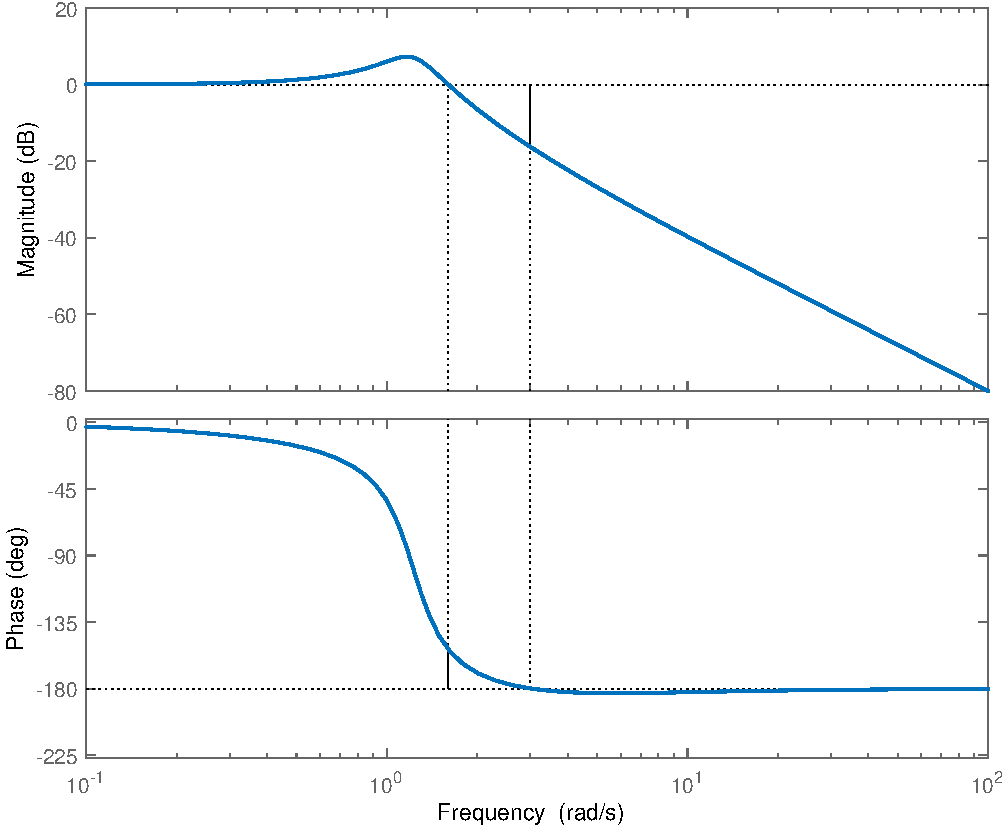
\includegraphics[width=1\textwidth]{chapter3/report_ch3_3_1}};
		\node (Wgc) at (-.8,0.5) {\small $\omega_{gc}$};
		\node (Wpc) at (.6,-0.5) {\small $\omega_{pc}$};		
		
		\node (GM) at (1.5,2.2) {\small $GM$};
	    \draw [-latex, ultra thick, black] (GM) -- (0.3,2.2);
		
		\node (PM) at (-1.6,-1.9) {\small $PM$};	    
	    \draw [-latex, ultra thick, black] (PM) -- (-0.5,-1.9);
	\end{tikzpicture}
	\end{minipage}%
	\hfill
	\begin{minipage}[t]{0.48\textwidth}
	\begin{tikzpicture}
		\node (img) {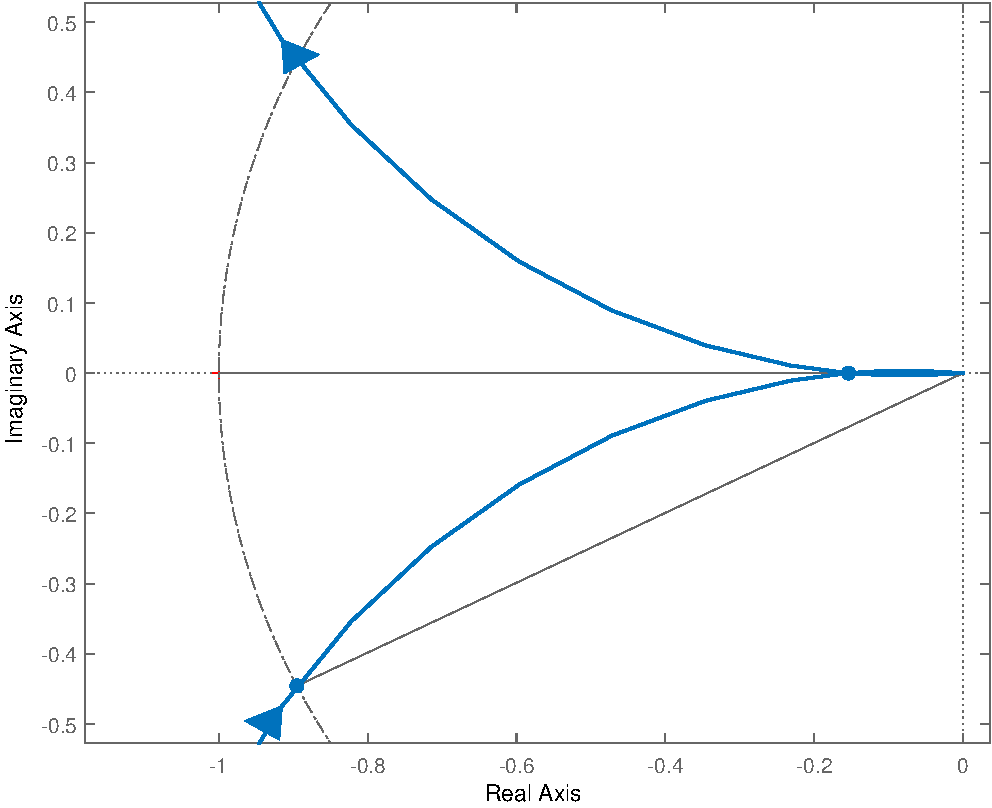
\includegraphics[width=1\textwidth]{chapter3/report_ch3_3_2}};
		\node (Wpc) at (3.1,0.5) {\small $\omega_{pc}$};
		\node (Wgc) at (-1.9,-2.1) {\small $\omega_{gc}$};		
		
		\node (GM) at (1.2,1.4) {\small $1 - \cfrac{1}{GM}$};
		\draw [-latex, <->] (-2.05,0.8) -- (2.65,0.8);
		\draw [-latex, -, dashed] (2.72,0.3) -- (2.72,1.1);
		\draw [-latex, -, dashed] (-2.12,0.3) -- (-2.12,1.1);
	    		
		\node (PM) at (-0.4, -0.5) {\small $PM$};	  
		\draw [-latex, <->] (0.5,-1.15) to[bend left] (0,0.2);  
	\end{tikzpicture}
	\end{minipage}%	
    
    \caption{Stability margins visualizations given Bode plots (left) and Nyquist diagrams (right) of closed-loop dynamical systems.}
    \label{fig:properties03}
\end{figure}

% The first property to be discussed is that of sensitivity \textbf{[reference]}. 

% \begin{boxed-definition}{(Sensitivity)} \label{def:sensitivity}
%   Consider a SISO system with state-feedback controller of gain $\bm{K}$ whose forward transfer function $\bm{G}_{f}(s)$ is given by \eqref{eq:fdbckForwardTrnsfer}. The \textit{sensitivity} function of this controlled system, denoted by the matrix $\bm{S}$, is defined as the transfer function from the system disturbances $\bm{D}_x(s)$ to the system total response, and it is equated as:
%   \begin{equation}
%       \bm{S}(s) = \left( \bm{I} + \bm{G}_f(s) \right)^{-1} = \cfrac{1}{1+G_f(s)}
%   \end{equation}
    
%   Additionally, the \textit{complementary sensitivity} function, denoted by the matrix $\bm{T}$, is defined as the transfer function from the reference to the state response, and it is equated as:
%   \begin{equation}
%       \bm{T}(s) = \left( \bm{I} + \bm{G}_f(s) \right)^{-1} \bm{G}_f(s) = \cfrac{G_f(s)}{1+G_f(s)}
%   \end{equation}
% \end{boxed-definition}

% This quantity states an important trade-off that has to be made when the feedback gain $\bm{K}$ is applied to a system subject to disturbances. To understand this, notice that:
% \begin{equation}
%   \bm{S} + \bm{T} = I
% \end{equation}

% Since both these quantities are transfer functions, a value of either one that is equal to the identity implies a perfect operation. Moreover, those values are directly affect by the increase or decrease of $\bm{K}$. This leads to the following observations:

% \begin{enumerate}
%   \item a
%   \item b
%   \item c
%   \item d
% \end{enumerate}

% 4 - Optimal Control and Estimation
% ---------------------------------------------------------------
\clearpage
\chapter{Optimal Control and Estimation}

This chapter introduces the vast field of optimal control and optimal estimation of dynamical systems. The developments are focused in optimizing a cost function that produces an optimal sequence of control actions to achieve the desired control objective, under some conditions. The chapter starts by discussing a general formulation of the optimal control problem and then specializes the formulation to a case of a linear system with quadratic cost functions. After that, the dual optimal state estimation problem is discussed and a result that merges the optimal control with the optimal estimation is presented. Finally, the main stability and robustness properties of the controllers derived in this chapter are accessed.

\section{Formulation}

The last chapter introduced the notion of controller synthesis as an engineering procedure to be done ``by hand" from a designer with some knowledge about the system and the control environment. This approach, despite being very popular and practical, is rather time-consuming and demands the designer to consider what are the best pole locations given some hard specifications. In addition to that, the design techniques previously presented becomes more involving when applied to MIMO systems. Thus, a more general and automatic procedure to control synthesis is desirable.

With this motivation, the concept of \textit{Optimal Control} \textbf{[references]} was introduced as an alternative strategy for controlling dynamical systems. Optimal controllers determines the necessary action by minimizing a cost function (or maximizing a reward function). These formulations produces feedback controllers that autonomously requires optimal input signals given a desired objective and possible restrictions, begin easily generalized to different systems \textbf{[reference]}.

\begin{boxed-definition}{(Optimal Control)} \label{def:optimalControl}
Given a system in State-Space formulation, with state signal $\bm{x} : \mathbb{R} \rightarrow \mathbb{R}^{n}$, and a reference signal $\bm{r} : \mathbb{R} \rightarrow \mathbb{R}^{n}$, the input signal $\bm{u}	(t) \in \mathbb{R}^r$, for any time $t$, is optimal if an optimal control law $\pi^* : \mathbb{R}^{n \times n \times 1} \rightarrow \mathbb{R}^r$ can be found as:
    \begin{equation}
        \bm{u}(t) = \pi^*(\bm{x}, \bm{r}, t) = \min_{\bm{u}} J(\bm{x}, \bm{r}, t)
    ,\end{equation}
    
\noindent where $J : \mathbb{R}^{n \times n \times 1} \rightarrow \mathbb{R}$ is known as a \textit{cost function} of the states and reference signals.
\end{boxed-definition}

Note that this optimization can be converted to maximizing a function $V(\cdot)$ by evaluating $V(\cdot) = -J(\cdot)$. Thus, this document will only refers to optimization as minimizing some cost function. The problem of finding an optimal control law, or optimal control policy, $\pi^*(\cdot)$ depends on the choice of the cost function $J(\cdot)$, and several optimization techniques can be used to determine the value of $\bm{u}(t)$ that achieve its minimum. This problem differs from standard optimization problems because it is dependent of time, there can be a decision variable and it is constrained by the dynamics of the model and by the optimal policy action. Solutions to this optimization can be obtained from several methods \textbf{[references]}. The approach used in this work focus on Dynamic Programming \textbf{[reference]}.

To facilitate the discussion and analysis of optimal controllers, consider a subclass of these controllers (that is still very general) defined below by a specific choice of functional for the cost function.

\begin{boxed-definition}{(Finite-Horizon Optimal Regulators)} \label{def:finiteHorizonOC}
    Consider a controller setup as in Definition \ref{def:optimalControl}. A \textit{Finite-Horizon Optimal Regulator} is defined as any controller whose optimal policy over a time interval $t \in [t_0, T]$ minimizes the cost functional:
    \begin{equation}
        J(\bm{x}, \bm{u}, t_0) = \int_{t_0}^T l(\bm{x}, \bm{u}, \tau) d \tau + l_f(\bm{x}, T)
    ,\end{equation}
    
    \noindent where $l(\cdot) : \mathbb{R}^{n \times r \times 1} \rightarrow \mathbb{R}$ and $l_f(\cdot) : \mathbb{R}^{n} \rightarrow \mathbb{R}$ are, respectively, the \textit{trajectory} and \textit{terminal loss functions}. In the case that $t_0 = 0$, $T$ is also known as the \textit{control horizon}.
\end{boxed-definition}

This formulation presents a notion of optimizing for a sequence of control actions $[\bm{u}(t_0), \cdots, \bm{u}(T)]$ that can cause a state trajectory $[\bm{x}(t_0), \cdots, \bm{x}(T)]$, which is optimal given the loss functions. As will be shown later, this is a very feasible strategy for controllable linear systems. In an optimization notation, this problem can also be presented as the following \textit{program}: 
\begin{align}
\begin{matrix*}[l]
    \text{minimize} & \int_{t_0}^T l(\bm{x}, \bm{u}, \tau) d \tau + l_f(\bm{x}, T) \\
    \hfill \text{s.t.} & \dot{\bm{x}}(t) = \bm{f}(\bm{x}, \bm{u}, t)  \\
                & \bm{u}(t) = \bm{pi}(\bm{x}(t_0), \cdots, \bm{x}(t))
\end{matrix*}
.\end{align}

Now, the discussion turns to how to solve this general problem. In this work, the solution for the optimal control will follow the dynamic programming formulation as in \textbf{[reference]}. The first necessary effort, then, is to define an important partial differential equation known as the Hamilton-Jacobi equation.

\begin{boxed-theorem}{(Hamilton-Jacobi equation)} \label{th:hamiltonJacobi}
    Consider a finite-horizon cost function in the form of Definition \ref{def:finiteHorizonOC}, for a system described by the state-equation $\dot{\bm{x}} = \bm{f}(\bm{x}, \bm{u}, t)$, restated as:
    \begin{equation} \label{eq:valueCostFunctional}
    	V(\bm{x}, \bm{u}, t_0) = \int_{t_0}^T l(\bm{x}, \bm{u}, \tau) d \tau + l_f(\bm{x}(T))
    \end{equation}
    
    \noindent Consider also that the loss $l(\cdot)$ and state function $\bm{f}$ are smooth on their parameters. Then, minimizing any functional in the form of $V(\cdot)$ is equivalent to determining the solution of the \textit{Hamilton-Jacobi equation}, which is given by the partial differential equation:
    \begin{equation} \label{eq:HJEquation}
        \cfrac{\partial V^*}{\partial t} = - \min_{u(t)} \left[ l(\bm{x}, \bm{u}, t) + \left[ \cfrac{\partial V^*}{\partial x} \right]^T \bm{f}(\bm{x}, \bm{u}, t)  \right]
    \end{equation}
    
    \noindent and the boundary condition:
    \begin{equation}
        V^*(\bm{x}, T) = l_f(\bm{x}(T))
    .\end{equation}
\end{boxed-theorem}

\begin{proof}
    First of all, consider the cost functional $V(\cdot)$ from \eqref{eq:valueCostFunctional}. Minimizing this functional with respect to the control inputs $\bm{u}(t_0), \cdots, \bm{u}(T)$ consists of evaluating the optimal cost:
    \begin{equation}
        V^*(\bm{x}, t_0) = \min_{\bm{u}(t_0), \cdots, \bm{u}(T)} \left[ \int_{t_0}^T l(\bm{x}, \bm{u}, \tau) d \tau + l_f(\bm{x}(T)) \right]
    .\end{equation}
    
    Now, consider any $t \in [t_0, T]$ and $t_r \in [t, T]$. Since the original control action $\bm{u}(t), \cdots, \bm{u}(T)$ can be obtained through the concatenation of $\bm{u}(t), \cdots, \bm{u}(t_r)$ and $\bm{u}(t_r), \cdots, \bm{u}(T)$, the optimal cost in this interval can be represented as:
    \begin{equation} \label{eq:HJERecursive}
    \begin{split}
    V^*(\bm{x}, t) &= \min_{\bm{u}(t), \cdots, \bm{u}(T)} \left[ \int_{t}^T l(\bm{x}, \bm{u}, \tau) d \tau + l_f(\bm{x}(T)) \right] \\
        &= \min_{\bm{u}(t), \cdots, \bm{u}(t_r)} \left\{ \min_{\bm{u}(t_r), \cdots, \bm{u}(T)} \left[ \int_{t}^{t_r} l(\bm{x}, \bm{u}, \tau) d \tau + \int_{t_r}^{T} l(\bm{x}, \bm{u}, \tau) d \tau + l_f(\bm{x}(T)) \right] \right\} \\
        &= \min_{\bm{u}(t), \cdots, \bm{u}(t_r)} \left\{ \int_{t}^{t_r} l(\bm{x}, \bm{u}, \tau) d \tau + \min_{\bm{u}(t_r), \cdots, \bm{u}(T)} \left[ \int_{t_r}^{T} l(\bm{x}, \bm{u}, \tau) d \tau + l_f(\bm{x}(T)) \right] \right\} \\
        &= \min_{\bm{u}(t), \cdots, \bm{u}(t_r)} \left\{ \int_{t}^{t_r} l(\bm{x}, \bm{u}, \tau) d \tau + V^*(\bm{x}, t_r) \right\}.
    \end{split}
    \end{equation}

	\noindent Notice that this is a recursive formula, since the optimal cost $V^*(\bm{x}, t)$ depends on $V^*(\bm{x}, t_r)$, which itself is an optimal cost for the future time $t_r \geq t$. Without loss of generalization, let $t_r = t + \delta t$, where $\delta t$ is a small number. Since $l(\cdot)$ is a smooth function, the right-hand side of the recursive form above can be expanded by a Taylor series expansion:
    \begin{equation}
    \begin{split}
        V^*(\bm{x}, t) = \min_{\bm{u}(t), \cdots, \bm{u}(t+\delta t)} & \biggl\{  l(\bm{x}, \bm{u}, t + \delta t) \delta t \biggr. \\ 
        & \left. + V^*(\bm{x}, t) + \left[ \cfrac{\partial V^*(\bm{x}, t)}{\partial \bm{x}} \right]^T \cfrac{d \bm{x}(t)}{dt} \delta t + \cfrac{\partial V^*(\bm{x}, t)}{\partial t} \delta t + \mathcal{O}(\delta t)^2  \right\}
    \end{split}
    ,\end{equation}
    
    \noindent where $\mathcal{O}(\delta t)^2$ denotes high order terms. Since the terms $V^*(\bm{x}, t)$ and $(\partial V^*/\partial t) \delta t$ do not depend on $\bm{u}(t)$, they can be disregarded of the minimization. Rearranging the terms and substituting $d \bm{x} / dt = \bm{f}(\bm{x}, \bm{u}, t)$ results in:
    \begin{equation}
        \cfrac{\partial V^*}{\partial t}(\bm{x}, t) =  - \min_{\bm{u}(t), \cdots, \bm{u}(t+\delta t)} \left\{ l(\bm{x}, \bm{u}, t + \delta t)  + \left[ \cfrac{\partial V^*(\bm{x}, t)}{\partial \bm{x}} \right]^T \bm{f}(\bm{x}, \bm{u}, t) + O(\delta t)^2  \right\}
    .\end{equation}
    
    Finally, letting $\delta t \to 0$ yields:
    \begin{equation}
        \cfrac{\partial V^*}{\partial t} =  - \min_{\bm{u}(t)} \left\{ l(\bm{x}, \bm{u}, t)  + \left[ \cfrac{\partial V^*}{\partial \bm{x}} \right]^T \bm{f}(\bm{x}, \bm{u}, t) \right\}
    .\end{equation}
    
    To prove the theorem it remains to derive the boundary condition. This result, however, is direct from the form of the cost function, since $V^*(\bm{x}, T) = l_f(\bm{x}(T))$ can not be changed through any more control action inside the time horizon.
\end{proof}

The Hamilton-Jacobi equation implies that finite-horizon optimal controllers can be optimized in a recursive manner, starting from the boundary condition at $t = T$ to the beginning of the horizon at $t = t_0$. This results from the fact that the last action $u(T)$ depends only on $l_f(\cdot)$, so it can be directly calculated for a desired final state $\bm{x}(T)$ and used to calculate the remaining optimal costs backward in time. This recursive property, directly evidenced in \eqref{eq:HJERecursive}, is a statement of the Bellman's Principle of Optimality \textbf{[reference]} and, for this reason, the Hamilton-Jacobi equation in the context of optimal control theory is known as the Hamilton-Jacobi-Bellman (HJB) equation. An illustration of this principle is shown in Fig. \ref{fig:generalOC01}

\begin{figure}[ht]
    \centering
    \resizebox{!}{!}{
    \begin{tikzpicture}[auto, node distance=1.75cm,>=latex', scale=0.2]
        % Nodes
        \node [mcCircle] (x0) {$x_0$};
        
        \node [mcCircle, right of=x0, node distance=8em] (x12) {};
        \node [mcCircle, above of=x12] (x11) {};
        \node [mcCircle, below of=x12] (x13) {};
        
        \node [mcCircle, right of=x12, node distance=12em] (xT) {$x_T$};
        
        % Scopes
        \begin{scope}[on background layer]
            \node [fit=(x11) (x13), fill= black!10, rounded corners, inner sep=.4cm, label={[xshift=0em, black!90]above:$x_1$}] {};
        \end{scope}         
        
        % Lines
        \draw [->, color=myRed!80, line width=.75mm] (x0) -- node[pos=0.7]{$70$} (x11);
        \draw [->] (x0) -- node[pos=0.6]{$40$} (x12);
        \draw [->] (x0) -- node[pos=0.45]{$130$} (x13);
        
        \draw [->, color=myRed!80, line width=.75mm, decorate, decoration={snake,amplitude=1.5mm, segment length=8mm}] (x11) -- node[pos=0.3]{$220$} (xT);
        \draw [->, decorate, decoration={snake,amplitude=1.5mm, segment length=8mm}] (x12) -- node[pos=0.4]{$270$} (xT);
        \draw [->, decorate, decoration={snake,amplitude=1.5mm, segment length=8mm}] (x13) -- node[pos=0.53]{$190$} (xT);
    \end{tikzpicture} 
    }
    \caption{Illustration of the Bellman's Principle of Optimality for a system with discrete set of states for a discrete time evolution. Each column represents a time instance and each node represents a possible state. The straight lines represents state transitions given an action with associated costs, whereas the curves represents the trajectory from that state to the terminal state with associated optimal cost. The optimal trajectory between the initial and terminal state is shown in red.}
    \label{fig:generalOC01}
\end{figure}

\section{Linear Quadratic (LQ) Controllers}

The last section introduced a general condition for solving a finite-horizon optimal control problem. Developing an analytical solution of that condition for any arbitrary loss function $l(\cdot)$ and state-equation $\bm{f}(\cdot)$ is usually intractable. However, there is a choice of loss function that, under a linear system, allows for a nice closed-form solution to the Hamilton-Jacobi-Bellman equation. This defines the popular class of optimal controllers known as the Linear Quadratic Controllers. Since these controllers are realizations of state-feedback controllers, this section discuss the two possible control operations presented in the last chapter, namely regulation and reference tracking. 

\subsubsection{Regulation}

\begin{boxed-definition}{(Linear Quadratic Regulator)} \label{def:lqr}
    Given a linear State-Space system in the form:
    \begin{align}
    \begin{cases}
        \dot{\bm{x}}(t) = \bm{A} \bm{x}(t) + \bm{B} \bm{u}(t) \\
        \bm{y}(t) = \bm{C} \bm{x}(t) + \bm{D} \bm{u}(t)
    \end{cases}
    .\end{align}
    
    A \textit{Linear Quadratic Regulator} (LQR) for this system is an optimal controller defined by the quadratic cost function:
    \begin{equation}
        J(\bm{x}, \bm{u}, t_0) = \int_{t_0}^{T} \left( \bm{x}^T \bm{Q} \bm{x} + \bm{u}^T \bm{R} \bm{u} \right) dt + \bm{x}^T(T) \bm{Q}_f \bm{x}(T)
    ,\end{equation}
    
    \noindent where is assumed that $\bm{Q},\bm{Q}_f  \succ 0$ and $\bm{R} \succ 0$ are matrices penalizing, respectively, the state-vector magnitude and the control effort.
\end{boxed-definition}

The LQR optimal controller was first introduced in \textbf{[reference]} and has been a foundation of optimal control theory ever since. From an engineering point of view, this choice of cost function has the advantage that it breaks the controller design to simply choose matrices $\bm{Q}$ and $\bm{R}$ as a trade-off between performance and actuator restrictions. From a mathematical point of view, the cost function has the advantage of being a quadratic function of the state and input signals, which is desirable since quadratic optimization problems have been widely studied in the literature \textbf{[reference]}. Now, it is necessary to develop a solution for the Hamilton-Jacobi equation in the light of this formulation. First of all, consider the following theorem.

\begin{boxed-theorem}{} \label{th:costQuadraForm}
    Consider a continuous cost function $V : \mathbb{R}^{n \times r \times 1} \rightarrow \mathbb{R}$ given by the LQR cost function defined in Definition \ref{def:lqr} for a linear system. The optimal cost $V^*(\bm{x}, t)$ has the quadratic form:
    \begin{equation}
        V^*(\bm{x}, t) = \bm{x}^T(t) \bm{P}(t) \bm{x}(t)
    \end{equation}
    
\noindent for any (possibly symmetric) matrix $\bm{P}(t)$ of appropriate dimensions. More precisely, the optimal cost $V^*(\bm{x}, t)$ satisfies the necessary and sufficient conditions for a quadratic function given as, for any $\lambda \in \mathbb{R}$:
    \begin{align} 
        V^*(\lambda \bm{x}, t) &= \lambda^2 V^*(\bm{x}, t) \label{eq:costQuadraForm021} \\ 
        V^*(\bm{x}_1 , t) + V^*(\bm{x}_2 , t) &= \cfrac{1}{2} \left( V^*(\bm{x}_1 + \bm{x}_2 , t) + V^*(\bm{x}_1 - \bm{x}_2 , t) \right) \label{eq:costQuadraForm022}
    .\end{align}
\end{boxed-theorem}

\begin{proof}
    Since $V^*(\bm{x}, t)$ is the minimum value of $V(\bm{x}, \bm{u}^*, t)$, given an optimal input $\bm{u}^*(t)$ for $t \in [t, T]$, then any deviation $\lambda \in \mathbb{R}$ in the parameters $(\bm{x},\ \bm{u}(t))$ will result in a greater value of the cost. A direct result from this and the fact that $V(\bm{x}, \bm{u}, t)$ is a quadratic function of $\bm{x}(t)$ and $\bm{u}(t)$ is that:
    \begin{equation}
        V^*(\bm{x}, t) \leq V(\lambda \bm{x}, \lambda \bm{u}^*, t) = \lambda^2 V^*(\bm{x}, t) \leq \lambda^2 V(\bm{x}, \lambda^{-1} \bm{u}^*, t) = V^*(\bm{x}, t)
    ,\end{equation}
    
    \noindent or, simply:
    \begin{equation}
        V^*(\bm{x}, t) \leq \lambda^2 V^*(\bm{x}, t) \leq V^*(\bm{x}, t)
    ,\end{equation}
    
    \noindent which directly implies $V^*(\bm{x}, t) = \lambda^2 V^*(\bm{x}, t)$ and establishes \eqref{eq:costQuadraForm021}. Similarly:
    \begin{align}
    \begin{split}
        V^*(\bm{x}_1, t) + V^*(\bm{x}_2, t) &= \cfrac{1}{4} \left( V^*(2 \bm{x}_1, t) + V^*(2 \bm{x}_2, t) \right) \\
            & \leq \cfrac{1}{4} \left( V(2 \bm{x}_1, \bm{u}_{x_1+x_2}^* + \bm{u}_{x_1-x_2}^*, t) + V(2 \bm{x}_2, \bm{u}_{x_1+x_2}^* - \bm{u}_{x_1-x_2}^*, t) \right) \\
            & = \cfrac{1}{2} \left( V(\bm{x}_1 + \bm{x}_2, \bm{u}_{x_1+x_2}^*, t) + V(\bm{x}_1 - \bm{x}_2, \bm{u}_{x_1-x_2}^*, t) \right) \\
            & = \cfrac{1}{2} \left( V^*(\bm{x}_1 + \bm{x}_2, t) + V^*(\bm{x}_1 - \bm{x}_2, t) \right) \leq V^*(\bm{x}_1, t) + V^*(\bm{x}_2, t),
    \end{split}
    \end{align}
    
    \noindent which implies $V^*(\bm{x}_1, t) + V^*(\bm{x}_2, t) = (1/2) \left( V^*(\bm{x}_1 + \bm{x}_2, t) + V^*(\bm{x}_1 - \bm{x}_2, t) \right)$ and establishes \eqref{eq:costQuadraForm022}. Therefore, the optimal cost function has a quadratic form $V^*(\bm{x}, t) = \bm{x}^T(t) \bm{P}(t) \bm{x}(t)$.
\end{proof}

This theorem shows that the fact that the cost function $V(\bm{x}, \bm{u}, t)$ is quadratic directly implies that the optimal cost $V^*(\bm{x}, t)$ is also quadratic. Therefore, it is possible to define the optimal action $\bm{u}^*(t)$ that produce this optimal cost by evaluating its relationship with the matrix $\bm{P}$. Since the quadratic cost just evaluated is defined for a finite-horizon optimal controller, it has to obey the condition imposed by the Hamilton-Jacobi equation, and the optimal controller can be solved as shown in the following theorem.

\begin{boxed-theorem}{(LQR Control Action)} \label{th:LQRAction}
    Given a Linear Quadratic Regulator as defined in Definition \ref{def:lqr}, the optimal action produced by this optimal controller at any time $t \in [t_0, T]$ is given by:
    \begin{equation}
        \bm{u}^*(t) = - \bm{R}^{-1} \bm{B}^T \bm{P}(t) \bm{x}(t)
    ,\end{equation}
    
    \noindent where $\bm{P}(t)$ is the solution of the matrix Riccati differential equation:
    \begin{equation}
        -\dot{\bm{P}}(t) = \bm{A}^T \bm{P}(t) + \bm{P}(t) \bm{A} - \bm{P}(t) \bm{B} \bm{R}^{-1} \bm{B}^T \bm{P}(t) + \bm{Q}
    ,\end{equation}
    
    \noindent with terminal condition $\bm{P}(T) = \bm{Q}_f$.
\end{boxed-theorem}

\begin{proof}
    Consider the Hamilton-Jacobi equation from \eqref{eq:HJEquation} restated below for a quadratic loss function $l(\bm{x}, \bm{u}, t$ and a linear system with state equation $\bm{f}(t)$ as given by Definition \ref{def:lqr}:
    \begin{equation}
    \begin{split}
        \cfrac{\partial (\bm{x}^T \bm{P} \bm{x})}{\partial t} &=  - \min_{\bm{u}(t)} \left\{ \bm{x}^T \bm{Q} \bm{x} + \bm{u}^T \bm{R} \bm{u} + \left[ \cfrac{\partial (\bm{x}^T \bm{P} \bm{x})}{\partial \bm{x}} \right]^T \left( \bm{A} \bm{x} + \bm{B} \bm{u} \right) \right\} \\
        \bm{x}^T \dot{\bm{P}} \bm{x} &= - \min_{\bm{u}(t)} \left\{ \bm{x}^T \bm{Q} \bm{x} + \bm{u}^T \bm{R} \bm{u} + (2 \bm{x}^T \bm{P}) \left( \bm{A} \bm{x} + \bm{B} \bm{u} \right) \right\}
    \end{split}
    ,\end{equation}
    
    \noindent where, without loss of generalization, $\bm{P}(t)$ was assumed to be symmetric. Because of the quadratic nature, it is possible to calculate the minimum of the right-hand side of the equation by taking its derivative with respect to the control action and equating it to zero:
    \begin{equation}
    \begin{split}
        0 &= \cfrac{\partial}{\partial \bm{u}(t)} \left( \bm{x}^T \bm{Q} \bm{x} + \bm{u}^T \bm{R} \bm{u} + (2 \bm{x}^T \bm{P}) \left( \bm{A} \bm{x} + \bm{B} \bm{u} \right) \right) \\
        0 &= 2 \bm{u}^T(t) \bm{R} + (2 \bm{x}^T(t) \bm{P}(t)) \bm{B} \\
        \bm{u}(t) &= - \bm{R}^{-1}  \bm{B}^T \bm{P}(t) \bm{x}(t)
    \end{split}
    .\end{equation}
    
    To solve for $\bm{P}$ first note that the following identity can be found by completing the squares:
    \begin{equation}
    \begin{split}
        \bm{x}^T \bm{Q} \bm{x} + \bm{u}^T \bm{R} \bm{u} + (2 \bm{x}^T \bm{P}) \left( \bm{A} \bm{x} + \bm{B} \bm{u} \right) = & (\bm{u} + \bm{R}^{-1} \bm{B}^T \bm{P} \bm{x})^T \bm{R} (\bm{u} + \bm{R}^{-1} \bm{B}^T \bm{P} \bm{x}) \\ & + \bm{x}^T (\bm{A}^T \bm{P} + \bm{P} \bm{A} - \bm{P} \bm{B} \bm{R}^{-1} \bm{B}^T \bm{P} + \bm{Q}) \bm{x}
    \end{split}
    .\end{equation}
    
\noindent Thus, substituting this identity and substituting the optimal control action results in the matrix Riccati equation:
    \begin{equation}
    \begin{split}
    \bm{x}^T \dot{\bm{P}} \bm{x} &= \bm{x}^T (\bm{A}^T \bm{P} + \bm{P} \bm{A} - \bm{P} \bm{B} \bm{R}^{-1} \bm{B}^T \bm{P} + \bm{Q}) \bm{x} \\
    \dot{\bm{P}} &= \bm{A}^T \bm{P} + \bm{P} \bm{A} - \bm{P} \bm{B} \bm{R}^{-1} \bm{B}^T \bm{P} + \bm{Q}
    \end{split}
    .\end{equation}
    
\noindent Finally, the terminal condition is direct from the fact that $V^*(\bm{x}, T) = \bm{x}^T(T) \bm{Q}_f \bm{x}(T)$.
\end{proof}

A closed-form solution for the LQR problem makes this controller a very appealing solution in several applications, since not only it is an optimal controller but the action can be calculated analytically. Several others optimal controllers may offer performance improvements, but usually depends on iterative optimization procedures, which can be computationally expensive to calculate for high-dimensional systems. Furthermore, the time complexity of the LQR control action computation is governed by the solution of the Riccati differential equation which can be done very efficiently \textbf{[reference]}.

Now, consider the optimal control action $\bm{u}^*(t)$. Applying this action to a linear system in State-Space representation results in the following state-equation:
\begin{equation}
\begin{split}
    \dot{\bm{x}}(t) &= \bm{A} \bm{x}(t) + \bm{B} \left( -\bm{R}^{-1} \bm{B}^T \bm{P}(t) \bm{x}(t) \right) \\
        & = \left( \bm{A} - \bm{B} \bm{R}^{-1} \bm{B}^T \bm{P}(t) \right) \bm{x}(t) \\
        & = \left( \bm{A} - \bm{B} \bm{K}(t) \right) \bm{x}(t)
\end{split}
.\end{equation}

This formulation indicates that the Linear Quadratic Regulator solution follows the exact same form of a general state-feedback regulator, represented by the linear but time-variant feedback system $\bm{A}_{cl}(t) = \left( \bm{A} - \bm{B} \bm{K}(t) \right)$. Notice, also, that both the computation of $\bm{K}(t)$ and $\bm{P}(t)$ does not explicitly depends on $\bm{x}(t)$, meaning that, for a specific control horizon, they can be calculated off-line and then provided to the controller actuator for the on-line operation. For this reason, despite being a closed-loop controller with corrective action, the LQR can be considered an open-loop optimizer, since the optimization solution itself does not depend on the state signal, but only on the system dynamical model.

\subsubsection{Reference Tracking}

As discussed in the previous chapter, the class of regulation controllers are broad but still restricted to a zero-state reference signal. To expand the range of application for the optimal controller just derived, it is possible to introduce integral action to the feedback.

\begin{boxed-definition}{(Linear Quadratic Servo)} \label{def:lqServo}
    Given a linear State-Space system represented by matrices $(\bm{A}, \bm{B}, \bm{C}, \bm{D})$, augmented with state $\dot{\bm{x}}_a(t) = \bm{r}(t) - \bm{C} \bm{x}(t)$:
    \begin{align} 
    \begin{cases}
        \begin{bmatrix}
            \dot{\bm{x}}(t) \\
            \dot{\bm{x}}_a(t)
        \end{bmatrix} &= \underbrace{\begin{bmatrix}
            \bm{A}  & \bm{0} \\ - \bm{C} & \bm{0}
        \end{bmatrix}}_{\tilde{\bm{A}}} \underbrace{\begin{bmatrix}
            \bm{x}(t) \\
            \bm{x}_a(t)
        \end{bmatrix}}_{\tilde{\bm{x}}(t)} + \underbrace{\begin{bmatrix}
            \bm{B} \\
            \bm{0}
        \end{bmatrix}}_{\tilde{\bm{B}}} \bm{u}(t) + \begin{bmatrix}
            \bm{0} \\
            \bm{I}
        \end{bmatrix} \bm{r}(t)
        \\
        \hfill \bm{y}(t) &= \begin{bmatrix}
            \bm{C} & \bm{0}
        \end{bmatrix} \begin{bmatrix}
            \bm{x}(t) \\
            \bm{x}_a(t)
        \end{bmatrix}
    \end{cases}
    .\end{align}
    
    A \textit{Linear Quadratic Servo} (LQ-Servo) for this system is an optimal controller defined by the quadratic cost function:
    \begin{equation}
        J(\bm{x}, \bm{u}, t_0) = \int_{t_0}^{T} \left( \tilde{\bm{x}}^T \tilde{\bm{Q}} \tilde{\bm{x}} + \bm{u}^T \bm{R} \bm{u} \right) dt +\tilde{\bm{x}} \tilde{\bm{Q}}_f \tilde{\bm{x}}(T)
    ,\end{equation}
    
    \noindent where is assumed that $\tilde{\bm{Q}}, \tilde{\bm{Q}}_f \succ 0$ and $\bm{R} \succ 0$ are matrices penalizing, respectively, the state-vector magnitude and the control effort.
\end{boxed-definition}

As before, the integral action turns the tracking problem into a regulation problem. In this case, the optimal controller will try to regulate towards a zero-state for $\bm{x}_a(t)$, yielding a zero error between the output $\bm{y}(t)$ and reference signal $\bm{r}(t)$. The new $p$ diagonal entries of the augmented matrix $\tilde{\bm{Q}}$ can be interpreted as weights penalizing the state deviation from the reference signal. The solution for this controller is the same as the one derived in Theorem \ref{th:LQRAction}, with $\bm{A} = \tilde{\bm{A}}$ and $\bm{B} = \tilde{\bm{B}}$. The resulting control action is equal to:
\begin{equation}
    \bm{u}(t) = \tilde{\bm{K}}(t)\tilde{\bm{x}}(t) = \begin{bmatrix} \bm{K}(t) & \bm{K}_a(t) \end{bmatrix} \begin{bmatrix} \bm{x}(t) \\ \bm{x}_a(t) \end{bmatrix}
.\end{equation}

\subsubsection{Infinite-Horizon LQ Controllers}

To conclude the section, it is also worth mentioning that, for the LQR cost function, it is possible to determine an optimal controller for an infinite-horizon operation, that is, when $T \to \infty$. The fact that the control horizon is now infinite results in a stationary state-feedback gain $\bm{K}$, as stated below.

\begin{boxed-theorem}{(Infinite-Horizon LQR)} \label{th:infiniteLQR}
    Consider a Linear Quadratic Regulator as defined in Definition \ref{def:lqr}, but with $T = \infty$. The optimal control action produced by this optimal controller at any time $t \in [t_0, \infty]$ is given by:
    \begin{equation}
        \bm{u}^*(t) = - \bm{K} \bm{x}(t) = - \bm{R}^{-1} \bm{B}^T \bm{P} \bm{x}(t)
    ,\end{equation}
    
    \noindent where $\bm{K} = \bm{R}^{-1} \bm{B}^T \bm{P}$ and $\bm{P}$ is the solution of the matrix algebraic Riccati equation:
    \begin{equation}
        \bm{0} = \bm{A}^T \bm{P} + \bm{P} \bm{A} - \bm{P} \bm{B} \bm{R}^{-1} \bm{B}^T \bm{P} + \bm{Q}
    .\end{equation}
\end{boxed-theorem}

A detailed proof of this result can be found in \textbf{[reference]}. The possibility for an infinite-horizon LQR is desirable in the sense that it doesn't restrict the operation to a fixed time interval, however, the resulting optimal controller suffers from a worst performance when compared to finite-time horizon controllers.

\section{Optimal State Estimators}

The state-vector $\bm{x}(t)$ is a necessary information to calculate $\bm{u}(t)$ in state-feedback controllers, but may also be inaccessible in practice. In Chapter 3, a deterministic observer, namely the Luenberger observer, was derived to deal with this problem. Despite being possible to utilize the Luenberger observer together with optimal controllers, this method suffers from the same design limitations of the Pole-Placement method, since they are dual problems. Therefore, this section develops an optimal state estimation approach which, from the estimation nature of the problem, relies on a statistical interpretation of the dynamical system and its observations. 

\subsubsection{General State Estimators}

First of all, consider a system perturbed by disturbances in the state-response and in the measurements, respectively $\bm{w} : \mathbb{R} \rightarrow \mathbb{R}^{n}$ and $\bm{v} : \mathbb{R} \rightarrow \mathbb{R}^{p}$. This configuration is illustrated at Fig. \ref{fig:optSE01}. If these disturbances are assumed to be zero-mean Gaussian variables, i.e., $\bm{w}_k \sim \mathcal{N}(\bm{0}, \bm{Q}_{kf})$ and $\bm{v}_k \sim \mathcal{N}(\bm{0}, \bm{R}_{kf})$ where $\bm{Q}_{kf}$ and $\bm{R}_{kf}$ are covariances matrices of appropriate sizes, then it is possible to motivate a stochastic formulation of the linear State-Space model. For the sake of simplicity, the discussion is focused on the discrete-time case. 

\begin{boxed-definition}{(Stochastic Discrete-Time State-Space)} \label{def:stochSS}
    Given an additive process noise variable $\bm{w}_k \sim \mathcal{N}(\bm{0}, \bm{Q}_{kf})$ with covariance $\bm{Q}_{kf} \in \mathbb{R}^{n \times n}$ and an additive measurement noise variable $\bm{v}_k \sim \mathcal{N}(\bm{0}, \bm{R}_{kf})$ with covariance $\bm{R}_{kf} \in \mathbb{R}^{p \times p}$, the stochastic discrete-time State-Space model is given by the equations:
    \begin{align}
    \left\{ \begin{matrix*}[l]
        \bm{x}_{k+1} = \bm{A}_d \bm{x}_k + \bm{B}_d \bm{u}_k + \bm{w}_k \\
        \bm{y}_{k\phantom{+1}} = \bm{C}_d \bm{x}_k + \bm{v}_k 
    \end{matrix*} \right.
    ,\end{align}
    
    \noindent for the initial condition $\bm{x}_0 \sim p(\bm{x}_0)$.
\end{boxed-definition}

\begin{figure}[ht]
    \centering
    \resizebox{!}{!}{
    \begin{tikzpicture}[auto, node distance=2cm,>=latex', scale=0.2]
        % We start by placing the blocks
        \node [input, name=input] {};
        \node [block, right of=input] (inputMatrix) {$\bm{B}$};
        \node [sum, right of=inputMatrix, node distance=4em] (stateSum) {};
        \node [block, right of=stateSum, node distance=6em] (integral) {$\bm{z}^{-1}$};        
        \node [input, above of=stateSum, node distance=4em] (wInput) {};
        \node [text width=1em, above of=wInput, node distance=1em] (wText) {$w_k$};
        \node [block, right of=integral, node distance=8em] (outputMatrix) {$\bm{C}$};
        \node [sum, right of=outputMatrix, node distance=4em] (vSum) {};
        \node [input, above of=vSum, node distance=4em] (vInput) {};
        \node [text width=1em, above of=vInput, node distance=1em] (vText) {$v_k$};
        \node [output, right of=vSum] (output) {};
        \node [block, below of=integral] (stateMatrix) {$\bm{A}$};
        
        \begin{scope}[on background layer]
            \node [fit=(inputMatrix) (stateMatrix) (vSum), fill= myBlue!10, rounded corners, inner sep=.4cm, label={[xshift=1.2em, myBlue!90]below left:Open-Loop System}] {};
        \end{scope}     
        
        % Once the nodes are placed, connecting them is easy.       
        \draw [draw,->] (input) -- node[pos=0.1] {$\bm{u}_k$} (inputMatrix);
        \draw [->] (inputMatrix) -- node[pos=0.8]{$+$} (stateSum);
        \draw [->] (stateSum) -- node[pos=0.6]{$\bm{x}_{k+1}$} (integral);
        \draw [->] (integral) -- node[name=bk1,pos=0.6]{$\bm{x}_{k}$} (outputMatrix);
        \draw [->] (wInput) -- node[pos=0.8]{$+$} (stateSum);
        \draw [->] (outputMatrix) -- node[pos=0.8]{$+$} (vSum);
        \draw [->] (vInput) -- node[pos=0.8]{$+$} (vSum);
        \draw [->] (vSum) -- node[pos=0.8]{$\bm{y}_k$} (output);
        \draw [->] (bk1) |- (stateMatrix);
        \draw [->] (stateMatrix) -| node[pos=0.95]{$+$} (stateSum);
    \end{tikzpicture} 
    }
    \caption{Block diagram of a stochastic discrete State-Space system.}
    \label{fig:optSE01}
\end{figure}

With this formulation, the noise variables can actually represent both the effect of external disturbances and the model uncertainty. This is important because dynamical models, even those developed according to a first-principle methodology, are not the true representation of the actual dynamical system or process. The motivation for a discussion of only a discrete State-Space model is to facilitate the interpretation of the statistical properties of the model. 

A direct result from Definition \ref{def:stochSS} is that, since $\bm{w}_k$ and $\bm{v}_k$ are random variables, $\bm{x}_k$ and $\bm{y}_k$ are also random variables. More precisely, since the noises variables are assumed to have a Gaussian distribution, both variables $\bm{x}_k \sim \mathcal{N}(\bm{\mu}_{x_k}, \bm{\Sigma}_{x_k})$ and $\bm{y}_k \sim \mathcal{N}(\bm{\mu}_{y_k}, \bm{\Sigma}_{y_k})$ are also Gaussian, where $\bm{\mu}_{x_k},\bm{\mu}_{y_k}$ are their respective mean vectors and $\bm{\Sigma}_{x_k},\bm{\Sigma}_{y_k}$ are the respective covariance matrices. This is because this distribution is closed to linear operations \textbf{[reference]}. For this reason, each state and output trajectory over a discrete time interval is a collection of time-indexed random variables following the Gaussian distribution, i.e., a stochastic process known as a Gaussian Process (GP) \textbf{[reference]}.

\begin{boxed-definition}{(Gaussian Process)} \label{def:gaussianProcess}
    Given a Gaussian process defined as a collection of random variables:
    \begin{equation}
        \bm{X} = \left\{ \bm{x}_k \sim \mathcal{N}(\mu_{\bm{x}_k}, \Sigma_{\bm{x}_k}) ; k \in [0,1,\cdots,K] \right\}
    .\end{equation}
    
    \noindent In the case that the variables represents states of a causal system, the joint probability of the random variables can be modeled as:
    \begin{equation} \label{eq:markovProp01}
        p(\bm{X}) = p(\bm{x}_0, \bm{x}_1, \cdots, \bm{x}_K) = \prod_{k=0}^K p(\bm{x}_k | \bm{x}_{k-1}, \cdots, \bm{x}_1, \bm{x}_0)
    .\end{equation}
\end{boxed-definition}

The defined joint probability $p(\bm{x}_0, \cdots, \bm{x}_K)$ is interpreted as the probability of a specific state trajectory to occur. The conditional probability $p(\bm{x}_k | \bm{x}_{k-1}, \cdots, \bm{x}_0)$ states that the probability associated with a random state variable $\bm{x}_k$ can be conditioned on the state trajectory $(\bm{x}_{k-1}, \cdots, \bm{x}_0)$ from the previous time instants. These two probabilities can be related through the well-known \textit{Chain Rule of Probability}, which, in the context of stochastic processes, is a realization of the \textit{Markov Property} \textbf{[reference]}. A nice property of Gaussian distributions is that the joint and condition distribution of Gaussian random variables are still Gaussian \textbf{[reference]}.


\subsubsection{Kalman Filter}

The dynamic response $\bm{x}_{k+1}$ of a system for a time instant $k+1$, given its trajectory until the actual state $\bm{x}_{k}$, is given by the conditional probability $p(\bm{x}_{k+1} | \bm{x}_{k}, \cdots, \bm{x}_1, \bm{x}_0)$. One can assume, however, that the an actual state stores enough information from the state trajectory until that point, that is possible to determine the next state response directly through its probability. Therefore, the conditional probability could be restated as:
\begin{equation}
    p(\bm{x}_{k+1} | \bm{x}_{k}, \cdots, \bm{x}_1, \bm{x}_0) =  p(\bm{x}_{k+1} | \bm{x}_{k})
.\end{equation}

A process that exhibits this property is known as a First-Order Markov process \textbf{[reference]}. With this formulation, it is always possible to marginalize the probability distribution of a random variable $\bm{x}_{k+1}$ given the initial state $\bm{x}_0$, which are related through the equation:
\begin{equation}
    p(\bm{x}_{k+1}) =  p(\bm{x}_{k+1} | \bm{x}_{k}) p(\bm{x}_{k} | \bm{x}_{k-1}) \cdots p(\bm{x}_{1} | \bm{x}_{0})p(\bm{x}_0) = p(\bm{x}_0) \prod_{i=0}^k p(\bm{x}_{i+1} | \bm{x}_{i})
.\end{equation}

\noindent Combining this assumption with Definition \ref{def:gaussianProcess}, in order to describe a Gauss-Markov Process, and using the model from Definition \ref{def:stochSS} it is possible to describe a stochastic dynamical system as the following probabilistic State-Space model.

\begin{boxed-definition}{(Controlled Hidden Markov Model)} \label{def:HMM}
    Given a stochastic State-Space model as in Definition \ref{def:stochSS}, and assuming the Markov property, a \textit{Controlled Hidden Markov Model} for this dynamical system at a time instant $k$ is defined through the two distributions:
    \begin{align}
    \begin{cases}
        p(\bm{x}_{k} | \bm{x}_{k-1}, \bm{u}_{k-1}) & \text{(Transition Distribution)} \\
        p(\bm{y}_{k} | \bm{x}_{k}) & \text{(Emission Distribution)}
    \end{cases}
    ,\end{align}
    
    \noindent for the initial condition given by $p(\bm{x}_0)$. Furthermore, since the noises $\bm{w}_k$ and $\bm{v}_k$ are zero-mean Gaussian noises, these distributions are modeled as the Normal conditional distributions:
    \begin{align}
    \left\{ \begin{matrix*}[l]
        p(\bm{x}_{k} | \bm{x}_{k-1}) = \mathcal{N}(\bm{x}_k | \bm{A}\bm{x}_{k-1} + \bm{B}\bm{u}_{k-1}, \bm{Q}_{kf}) \\
         p(\bm{y}_{k} | \bm{x}_{k})\phantom{_{-1}} = \mathcal{N}(\bm{y}_k | \bm{C}\bm{x}_{k}, \bm{R}_{kf}) \hfill
    \end{matrix*} \right.
    .\end{align}
\end{boxed-definition}

A Hidden-Markov Model is a statistical interpretation of dynamical system that is well-known in the literature \textbf{[reference?]}. An illustration of the dependence between these variables as a graphical model is depicted in Fig. \ref{fig:HMM01}. Notice that, in this formulation, the state-vector $\bm{x}_k$ actual value is never known (since it is a latent variable), but can be observed through the emission variable $\bm{y}_k$, under the assumption that system model is perfectly known. This raises the problem of state estimation as a common inference problem known as the \textit{filtering}, which consists on determining statistically the actual value of $\bm{x}_k$ given the observations $\bm{y}_0, \cdots, \bm{y}_k$ and control actions $\bm{u}_0, \cdots, \bm{u}_k$. Thus, the state can be obtained through the distribution:
\begin{equation}
    p(\bm{x}_k | \bm{y}_{k}, \bm{y}_{k-1}, \cdots, \bm{y}_0, \bm{u}_{k-1}, \bm{u}_{k-2}, \cdots, \bm{u}_0)
,\end{equation}

\noindent from which a representative value, such as the expected value $\mathbb{E}\left[ p(\bm{x}_k | \bm{y}_{k}, \cdots, \bm{y}_0, \bm{u}_{k-1}, \cdots, \bm{u}_0) \right]$ can be selected.

\begin{figure}[ht]
    \centering
    \resizebox{!}{!}{
    \begin{tikzpicture}[auto, node distance=1.9cm,>=latex', scale=0.2]
        % Nodes
        \node [mcInput] (u0) {$u_0$};
        \node [mcCircleX, below of=u0] (x0) {$x_0$};
        \node [mcCircleY, below of=x0] (y0) {$y_0$};
        
        \node [mcInput, right of=u0] (u1) {$u_1$};
        \node [mcCircleX, below of=u1] (x1) {$x_1$};
        \node [mcCircleY, below of=x1] (y1) {$y_1$};
        
        \node [text width=2em, right of=x1] (cdots1) {$\cdots$};    
        
		\node [mcCircleX, right of=cdots1] (xi1) {$x_{k-1}$};     
        \node [mcInput, above of=xi1] (ui1) {$u_{k-1}$};
        \node [mcCircleY, below of=xi1] (yi1) {$y_{k-1}$};        
        
        \node [mcCircleX, right of=xi1] (xi2) {$x_{k}$};     
        \node [mcInput, above of=xi2] (ui2) {$u_{k}$};
        \node [mcCircleY, below of=xi2] (yi2) {$y_{k}$};
        
		\node [mcCircleX, right of=xi2] (xi3) {$x_{k+1}$};     
        \node [mcInput, above of=xi3] (ui3) {$u_{k+1}$};
        \node [mcCircleY, below of=xi3] (yi3) {$y_{k+1}$};        
        
        \node [text width=2em, right of=xi3] (cdots2) {$\cdots$};
        
        \node [mcCircleX, right of=cdots2] (xk) {$x_K$};
        \node [mcCircleY, below of=xk] (yk) {$y_K$};
        
        % Lines
        \draw [->,line width=.5mm] (u0) -- (x1);
        \draw [->,line width=.5mm] (u1) -- (cdots1);
        \draw [->,line width=.5mm] (ui1) -- (xi2);
        \draw [->,line width=.5mm] (ui2) -- (xi3);
        \draw [->,line width=.5mm] (ui3) -- (cdots2);
        
        \draw [->,line width=.5mm] (x0) -- (x1);
        \draw [->,line width=.5mm] (x1) -- (cdots1);
        \draw [->,line width=.5mm] (cdots1) -- (xi1);
        \draw [->,line width=.5mm] (xi1) -- (xi2);
        \draw [->,line width=.5mm] (xi2) -- (xi3);
        \draw [->,line width=.5mm] (xi3) -- (cdots2);
        \draw [->,line width=.5mm] (cdots2) -- (xk);
       
        \draw [->,line width=.5mm] (x0) -- (y0);
        \draw [->,line width=.5mm] (x1) -- (y1);
        \draw [->,line width=.5mm] (xi1) -- (yi1);
        \draw [->,line width=.5mm] (xi2) -- (yi2);
        \draw [->,line width=.5mm] (xi3) -- (yi3);
        \draw [->,line width=.5mm] (xk) -- (yk);
    \end{tikzpicture} 
    }
    \caption{A Controlled Hidden Markov Model for a discrete-time system, where the shaded boxes indicates that the inputs are not random variables.}
    \label{fig:HMM01}
\end{figure}

There are several approaches to solve the filtering and other related problems in statistical state estimation \textbf{[reference-Sarkka]}, but the most popular method has been the Kalman filter \textbf{[reference]} which is discussed below for a discrete-time system.

\begin{boxed-theorem}{(Kalman Filter)} \label{th:kalmanFilter}
    Given a Controlled Hidden Markov Model as in Definition \ref{def:HMM} and initial state distribution $\bm{x}_0 \sim \mathcal{N}(\bar{x}_0, \bm{P}_0)$, the filtering distribution can be solved in closed-form as:
    \begin{equation}
        p(\bm{x}_k | \bm{y}_{k}, \cdots, \bm{y}_0, \bm{u}_{k-1}, \cdots, \bm{u}_0)  = \mathcal{N}(\bar{\bm{x}}_k, \bm{P}_k)
    ,\end{equation}   
    
    \noindent where $\bar{x}_k$, which denotes the mean of $\bm{x}_k$, and covariance $\bm{P}_k$ are recursively computed through the prediction and update steps below.
    \begin{itemize}
    	\item Prediction Step:
    	\begin{align}
	    \begin{matrix*}[l]
		    \hat{\bar{\bm{x}}}_k = \bm{A} \bar{\bm{x}}_{k-1} + \bm{B} \bm{u}_{k-1},  \\
		    \hat{\bm{P}}_k = \bm{A} \bm{P}_{k-1} \bm{A}^T + \bm{Q_{kf}}.
		\end{matrix*}
		\end{align}
		
		\item Update Step:
		\begin{align}
	    \begin{matrix*}[l] 
		    \bm{K}_k = \hat{\bm{P}}_k \bm{C}^T (\bm{R}_{kf} + \bm{C} \hat{\bm{P}}_k \bm{C}^T)^{-1} ,\\
		    \bar{\bm{x}}_k = \hat{\bar{\bm{x}}}_k + \bm{K}_k(\bm{y}_k - \bm{C} \hat{\bar{\bm{x}}}_k), \\
		    \bm{P}_k = \hat{\bm{P}}_k - \bm{K}_k (\bm{R}_{kf} + \bm{C} \bar{\bm{P}}_k \bm{C}^T) \bm{K}_k^T.
	    \end{matrix*}   
	    \end{align}
	    \end{itemize}
\end{boxed-theorem}

\begin{proof}
    Consider the transition and emission distributions given as:
    \begin{align}
    \left\{ \begin{matrix*}[l]
        p(\bm{x}_{k} | \bm{x}_{k-1}) = \mathcal{N}(\bm{x}_k | \bm{A}\bar{\bm{x}}_{k-1} + \bm{B}\bm{u}_{k-1}, \bm{Q}_{kf}) \\
         p(\bm{y}_{k} | \bm{x}_{k})\phantom{_{-1}} = \mathcal{N}(\bm{y}_k | \bm{C}\bar{\bm{x}}_{k}, \bm{R}_{kf}) \hfill
    \end{matrix*} \right.
    .\end{align}
    
    \noindent Consider, now, the distribution of $\left( \bm{x}_{k-1}, \bm{x}_k \right)$ conditioned on measurements $\left( \bm{y}_0, \bm{y}_1, \cdots, \bm{y}_{k-1} \right)$. Since the joint and condition distributions of a Gaussian are themselves Gaussian, this density can be expressed as:
    \begin{align}
    \begin{split}
        p(\bm{x}_k, \bm{x}_{k-1} | \bm{y}_0, \bm{y}_1, \cdots, \bm{y}_{k-1}) &= p(\bm{x}_k | \bm{x}_{k-1}) p(\bm{x}_{k-1} | \bm{y}_0, \bm{y}_1, \cdots, \bm{y}_{k-1}) \\
        &= \mathcal{N}(\bm{x}_k | \bm{A}\bar{\bm{x}}_{k-1}+\bm{B}\bm{u}_{k-1}, \bm{Q}_{kf}) \mathcal{N}(\bm{x}_{k-1} | \bar{\bm{x}}_{k-1}, \bm{P}_{k-1}) \\
        &= \mathcal{N}\left( \begin{bmatrix} \bm{x}_{k-1} \\ \bm{x}_{k} \end{bmatrix}    \right| \left. \begin{bmatrix} \bar{\bm{x}}_{k-1} \\ \bm{A}\bar{\bm{x}}_{k-1}+\bm{B}\bm{u}_{k-1} \end{bmatrix}, \begin{bmatrix} \bm{P}_{k-1} & \bm{P}_{k-1} \bm{A}^T  \\ \bm{A} \bm{P}_{k-1} & \bm{A} \bm{P}_{k-1} \bm{A}^T + \bm{Q}_{kf} \end{bmatrix}  \right).
    \end{split}
    \end{align}
    
    Marginalizing the joint distribution, it is possible to obtain the distribution of $\bm{x}_k$ conditioned in the measurement history as:
    \begin{equation}
        p(\bm{x}_k | \bm{y}_0, \bm{y}_1, \cdots, \bm{y}_{k-1}) = \mathcal{N}( \underbrace{\bm{A} \bar{\bm{x}}_{k-1} + \bm{B} \bm{u}_{k-1}}_{\hat{\bar{\bm{x}}}_k}, \underbrace{\bm{A} \bm{P}_{k-1} \bm{A}^T + \bm{Q}_{kf}}_{\hat{\bm{P}}_k} )
    ,\end{equation}
    
    \noindent which completes the \textit{prediction step} of the Kalman filter. For the update step, consider the joint distribution between $(\bm{x}_k, \bm{y}_k)$, the actual state and actual measurement, which applying Lemma \ref{le:jointGauss} results in:
    \begin{align}
    \begin{split}
        p(\bm{x}_k, \bm{y}_{k} | \bm{y}_0, \bm{y}_1, \cdots, \bm{y}_{k-1}) &= p(\bm{y}_k | \bm{x}_{k}) p(\bm{x}_{k} | \bm{y}_0, \bm{y}_1, \cdots, \bm{y}_{k-1}) \\
        &= \mathcal{N}(\bm{y}_k | \bm{C}\bar{\bm{x}}_{k}, \bm{R}_{kf}) \mathcal{N}(\bm{x}_{k} | \hat{\bar{\bm{x}}}_k, \hat{\bm{P}}_k) \\
        &= \mathcal{N}\left( \begin{bmatrix} \bm{x}_{k} \\ \bm{y}_{k} \end{bmatrix}  \right| \left. \begin{bmatrix} \hat{\bar{\bm{x}}}_k \\ \bm{C}\hat{\bar{\bm{x}}}_k \end{bmatrix}, \begin{bmatrix} \hat{\bm{P}}_k & \hat{\bm{P}}_k \bm{C}^T  \\ \bm{C} \hat{\bm{P}}_k & \bm{C} \hat{\bm{P}}_k \bm{C}^T + \bm{R}_{kf} \end{bmatrix}   \right).
    \end{split}
    \end{align}
    
    Therefore, using Lemma \ref{le:condGauss}, the filtering distribution can be obtained as:
    \begin{align}
        p(\bm{x}_k | \bm{y}_k, \bm{y}_0, \bm{y}_1, \cdots, \bm{y}_{k-1}) = \mathcal{N}(\bm{x}_k | \bar{\bm{x}}_k, \bm{P}_k)
    ,\end{align}

    \noindent where $\hat{\bm{x}}_k$ and $\bm{P}_k$ are the computations of the update step, given as:
    \begin{align}
    \begin{cases}
        \bar{\bm{x}}_k = \hat{\bar{\bm{x}}}_k + \hat{\bm{P}}_k \bm{C}^T (\bm{R}_{kf} + \bm{C} \hat{\bm{P}}_k \bm{C}^T)^{-1}(\bm{y}_k - \bm{C}\hat{\bar{\bm{x}}}_k) \\
        \bm{P}_k = \hat{\bm{P}}_k - \hat{\bm{P}}_k \bm{C}^T (\bm{R}_{kf} + \bm{C} \hat{\bm{P}}_k \bm{C}^T)^{-1} \bm{C} \hat{\bm{P}}_k
    \end{cases}
    .\end{align}
    
    \noindent Finally, making $\bm{K}_k = \hat{\bm{P}}_k \bm{C}^T (\bm{R}_{kf} + \bm{C} \hat{\bm{P}}_k \bm{C}^T)^{-1}$ concludes the proof.
\end{proof}

Notice that the Kalman filter solution implies that an ``open-loop" estimation of the mean of the states, $\hat{\bar{\bm{x}}}_k$, can be corrected by the equation:
\begin{equation}
    \bar{\bm{x}}_k = \hat{\bar{\bm{x}}}_k + \bm{K}_k (\bm{y}_k - \bm{C} \hat{\bar{\bm{x}}}_k)
,\end{equation}

\noindent which, by expanding $\hat{\bar{\bm{x}}}_k$, results in a similar state-equation expression for a system with a deterministic observer as defined earlier, but for a time-varying gain $\bm{K}_k$:
\begin{equation}
\begin{split}
    \bar{\bm{x}}_k &= \bm{A} \bar{\bm{x}}_k + \bm{B} \bm{u}_k + \bm{K}_k (\bm{y}_k - \bm{C} \hat{\bar{\bm{x}}}_k) \\
    &= \left( \bm{A} - \bm{K}_k \bm{C} \right) \bar{\bm{x}}_k + \bm{B} \bm{u}_k + \bm{K}_k \bm{y}_k
\end{split}
.\end{equation}

Notice that, despite the similarity with Luenberger observers, the Kalman gain has the advantage that the gain matrix $\bm{K}_k$ is not resulting from a designer procedure but rather from solving an inference problem whose only additional information needed are the covariances $\bm{Q}_{kf}$ and $\bm{R}_{kf}$, which can be assumed or estimated. 

\subsubsection{Controller-Estimator Duality}

In addition to that, it can be shown that the recursive steps that solves the filtering problem are also responsible for iteratively minimizing the trace of the covariance matrix $\bm{P}_k$ [reference], which is given as:
\begin{equation}
    \bm{P}_k = \mathbb{E}\left[ (\bm{x}_k - \bar{\bm{x}}_k)(\bm{x}_k - \bar{\bm{x}}_k)^T \right]
.\end{equation}

\noindent Since this method minimizes some cost function, it is indeed an optimal estimator. In fact, the Kalman filter can be formulated through an optimal control formulation, which motivates the development of a continuous-time version of this estimator, as shown below.

\begin{boxed-theorem}{(Kalman-Bucy Filter)} \label{th:kalmanBucy}
    Consider a continuous-time State-Space linear system subject to additive process noise variable $\bm{w}_k \sim \mathcal{N}(\bm{0}, \bm{Q}_{kf})$ and measurement noise variable $\bm{v}_k \sim \mathcal{N}(\bm{0}, \bm{R}_{kf})$, where the covariances $\bm{Q}_{kf} \in \mathbb{R}^{n \times n}$  and $\bm{R}_{kf} \in \mathbb{R}^{p \times p}$ represents the \emph{power spectral density} of the noises. In this case, for an estimated state $\bar{\bm{x}}(t)$ at time $t$, the error covariance:
    \begin{equation}
        \bm{J}(\bm{x}, \bar{\bm{x}}, t) = \mathbb{E}\left\{ [\bm{x}(t) - \bar{\bm{x}}(t)][\bm{x}(t) - \bar{\bm{x}}(t)]^T \right\}
    \end{equation}
    
    \noindent is minimized by $\bar{\bm{x}}(t)$ obtained through the system:
    \begin{equation}
        \dot{\bar{\bm{x}}}(t) = \bm{A} \bar{\bm{x}}(t) + \bm{B} \bm{u}(t) + \bm{K}_{e}(t) \left( \bm{y}(t) - \bm{C} \bar{\bm{x}}(t) \right)
    ,\end{equation}
    
    \noindent where $\bm{K}_e(t) = \bm{P}_e(t)\bm{C}\bm{R}^{-1}$, being $\bm{P}_e(t)$ the solution of the Riccati differential matrix equation:
    \begin{equation}
        \dot{\bm{P}_e}(t) = \bm{A} \bm{P}_e(t) + \bm{P}_e(t) \bm{A}^T - \bm{P}_e(t)\bm{C}^T\bm{R}_{kf}^{-1} \bm{C} \bm{P}_e(t) + \bm{Q}_{kf}
    ,\end{equation}
    
    \noindent with initial condition $\bm{P}_e(t_0) = \mathbb{E} \left\{ [\bm{x}(t_0) - \bar{\bm{x}}(t_0)][\bm{x}(t_0) - \bar{\bm{x}}(t_0)]^T \right\}$ for $t_0 > -\infty$.
\end{boxed-theorem}

A detailed proof of this theorem can be found in \textbf{[reference]}. The formulation of an optimal state estimator further emphasizes the duality between controllers and observers. Notice that the gain $\bm{K}_e(t)$ of a Kalman-Bucy filter depends on a matrix $\bm{P}_e(t)$ that solves the exact same Riccati differential equation as the one in Theorem \ref{th:LQRAction}, but forward in time for matrices $\bm{A}^T$ and $\bm{C}^T$ instead of $\bm{A}$ and $\bm{B}$. Notice, however, that these filters are not limited to a terminal time $T$, since the boundary condition only requires information on the initial time $t_0 > -\infty$, which implies that they could also be used in forward infinite-horizon operations. Another direct result of the duality is that is possible to derive an estimator considering $t_0 \to -\infty$, which, as in Theorem \ref{th:infiniteLQR}, results in a time-invariant filter with gain $K_e$ \textbf{[reference]}.

\section{Linear Quadratic Gaussian (LQG)}

This chapter presented formulation for controllers and state estimators that are optimal, in the sense that they minimize some cost function based on information about the model and measurements. In the previous chapter, the Theorem \ref{th:separationPrinciple} stated that a controller and an estimator can be designed separately, and a resulting control by feedback of estimated states is always feasible. In this section, a similar configuration is shown for optimal control and estimation operations, as depicted in Fig. \ref{fig:lqg01}. 

\begin{figure}[ht]
    \centering
    \resizebox{\textwidth}{!}{
    \begin{tikzpicture}[auto, node distance=2cm,>=latex']
        % We start by placing the blocks
        \node [input, name=input] {};
        \node [sum, right of=input, node distance=3em] (intFbckSum) {};
        \node [block, right of=intFbckSum, node distance=4em] (integralAction) {$\int$};
        \node [block, right of=integralAction, node distance=6em] (intActGain) {$\bm{K}_a$};
        \node [sum, right of=intActGain, node distance=4.5em] (fbckSum) {};

        \node [block, fill=myBlue!20, minimum height=4em, right of=fbckSum, node distance=14em] (openloopSystem) {Open-Loop System};    
        \node [output, right of=outputMatrix, node distance=25em] (output) {};
        
        \node [block, below of=openloopSystem, node distance=12.5em] (integralLU) {$\int$};     
        \node [sum, left of=integralLU, node distance=4em] (stateSumLU) {};             
        \node [block, left of=stateSumLU, node distance=4em] (inputMatrixLU) {$\bm{B}$};
        \node [block, right of=integralLU, node distance=8em] (outputMatrixLU) {$\bm{C}$};
        \node [block, below of=integralLU] (stateMatrixLU) {$\bm{A}$};
        \node [block, above of=integralLU] (kalmanGain) {$\bm{K}_e$};       
        
        \draw [->] (openloopSystem) -- node[name=bk3,pos=0.5]{} node[name=bk5,pos=0.75]{} node[pos=0.9]{$\bm{y}$} (output);
        \node [sum, anchor=base] (fbckOutput) at (bk3.base |- kalmanGain) {};
        
        \node [block, below of=stateSumLU, node distance=11em, label={below:LQR Controller}] (fbckGain) {$\bm{K}$};     
        
        
        \begin{scope}[on background layer]
            \node [fit=(integralAction) (intActGain), fill= myGreen!10, rounded corners, inner sep=.4cm, label={[xshift=4.3em, myGreen!90]above left:Integral Action}] {};
        \end{scope} 
        
        \begin{scope}[on background layer]
            \node [fit=(inputMatrixLU) (kalmanGain) (stateMatrixLU) (fbckOutput), fill= myRed!10, rounded corners, inner sep=.4cm, label={[xshift=5.8em, myRed!90]above left:Kalman-Bucy Filter}] {};
        \end{scope} 
        
        % Once the nodes are placed, connecting them is easy.       
        \draw [draw,->] (input) -- node[pos=0.1] {$\bm{r}$} node[pos=0.8] {$+$}  (intFbckSum);
        \draw [->] (intFbckSum) -- (integralAction);
        \draw [->] (integralAction) -- node[pos=0.5]{$\bm{x}_a$} (intActGain);
        \draw [->] (intActGain) -- node[pos=0.8]{$-$} (fbckSum);        
        \draw [->] (fbckSum) -- node[pos=0.2]{$\bm{u}$} node[name=bku1, pos=0.2]{} (openloopSystem);
        

        \draw [->] (fbckGain) -| node[pos=0.98]{$-$} (fbckSum);
        \draw [->] (bk5) |- ++(0, -28em) -| node[pos=0.98]{$-$} (intFbckSum);
        
        
        \draw [->] (bku1) |- (inputMatrixLU);
        \draw [->] (inputMatrixLU) -- node[pos=0.8]{$+$} (stateSumLU);
        \draw [->] (stateSumLU) -- node[pos=0.5]{$\dot{\hat{\bm{x}}}$} (integralLU);
        \draw [->] (integralLU) -- node[name=bk4,pos=0.5]{} node[pos=0.5]{$\hat{\bm{x}}$} (outputMatrixLU);
        \draw [->] (outputMatrixLU) -| node[pos=0.95]{$-$} (fbckOutput);
        \draw [->] (bk4) |- (stateMatrixLU);
        \draw [->] (fbckOutput) -- (kalmanGain);
        \draw [->] (stateMatrixLU) -| node[pos=0.95]{$+$} (stateSumLU);
        \draw [->] (kalmanGain) -| node[pos=0.95]{$+$} (stateSumLU);
        \draw [->] (bk3) -- node[pos=0.95]{$+$} (fbckOutput);
        
        \draw [->] (bk4) |- (fbckGain);
    \end{tikzpicture} 
    }
    \caption{Block diagram of a Linear Quadratic Gaussian control configuration.}
    \label{fig:lqg01}
\end{figure}

The control configuration that connects an optimal control action of a Linear Quadratic Regulator together with the estimation states from a Kalman filter (or Kalman-Bucy filter) is know as a Linear Quadratic Gaussian (LQG) controller \textbf{[reference]}. Since the controller is independent of the estimator, it is also possible to include integral action to the configuration, as shown in the block diagram, presenting this architecture as a general configuration that can deal with a broad range of applications. Because of the stochastic nature of the estimation and the optimal procedure of the control, this configuration is central to the field of Stochastic Optimal Control \textbf{[reference?]}. A formal definition is given below.

\begin{boxed-definition}{(Linear Quadratic Gaussian)} \label{def:lqg}
    Consider a stochastic system in State-Space representation just as in Definition \ref{def:stochSS}, rewritten below:
	\begin{align}
    \begin{cases}
        \hfill \dot{\bm{x}}(t) &= \bm{A} \bm{x}(t) + \bm{B} \bm{u}(t) + \bm{w}(t) \\
        \hfill \bm{y}(t) &= \bm{C} \bm{x}(t) + \bm{v}(t)
    \end{cases}
    ,\end{align}
    
     \noindent whose estimated state-vector $\hat{\bm{x}}(t)$ is determined by a Kalman-Bucy filter and whose optimal input signal $\bm{u}(t)$ is calculated through a finite-horizon LQR. The Linear Quadratic Gaussian (LQG) control for the horizon $t \in [t_0, T]$, with $-\infty < t_0 \leq T < \infty$, is defined as:
    \begin{align} \label{eq:lqg01}
        \dot{\hat{\bm{x}}}(t) = \left[\bm{A} - \bm{K}_e(t) \bm{C} - \bm{B} \bm{K}(t) \right] \hat{\bm{x}}(t) + \bm{K}_e(t) \bm{y}(t) 
    ,\end{align}
    
    \noindent where $\bm{K}(t) = \bm{R}^{-1}\bm{B}^T \bm{P}(t)$ and $\bm{K}_e(t) = \bm{P}_e(t) \bm{C} \bm{R}^{-1}$ are, respectively, the LQR and Kalman-Bucy gains for matrices $\bm{P}(t)$ and $\bm{P}_e(t)$ that solve the Riccati differential equations:
    \begin{align}
    \begin{cases}
        -\dot{\bm{P}}(t) = \bm{A}^T \bm{P}(t) + \bm{P}(t) \bm{A} - \bm{P}(t) \bm{B} \bm{R}^{-1} \bm{B}^T \bm{P}(t) + \bm{Q} \\
        \phantom{-} \dot{\bm{P}_e}(t) = \bm{A} \bm{P}_e(t) + \bm{P}_e(t) \bm{A}^T - \bm{P}_e(t)\bm{C}^T\bm{R}_{kf}^{-1} \bm{C} \bm{P}_e(t) + \bm{Q}_{kf}
    \end{cases}
    \end{align}
    
    \noindent for boundary conditions $\bm{P}(T) = \bm{Q}_f$ and $\bm{P}_e(t_0) = \mathbb{E} \left\{ [\bm{x}(t_0) - \bar{\bm{x}}(t_0)][\bm{x}(t_0) - \bar{\bm{x}}(t_0)]^T \right\}$, respectively.
\end{boxed-definition}

Notice that another advantage of this controller-estimator configuration is that the solution for both Riccati differential equations does not depends on the states at any time $\bm{x}(t)$, with the exception of the boundary condition $\bm{P}_e(t_0)$ which can in any case be obtained before the system operation. Therefore, the values for matrices $\bm{P}(t)$ and $\bm{P}_e(t)$, and consequently $\bm{K}(t)$ and $\bm{K}_e(t)$, for $t \in [t_0, T]$, can be evaluated beforehand and then applied in the on-line operation.

The LQG controller can also be used for tracking non-constant references, given that the system can be augmented while maintaining controllability. The augmented system is used to calculate the controller gains $\bm{K}(t)$ using Definition \ref{def:lqServo}, while the estimator gains $\bm{K}_e(t)$ are optimized through the original system. Given that it can optimally solve both the regulator and tracking problems, while still accounting for uncertainty in the system, the Linear Quadratic Gaussian poses as a high performing multi-purpose controller. The resulting augmented system can be represented by the closed-loop state equation:
\begin{align}
\begin{cases}
        \begin{bmatrix}
            \dot{\hat{\bm{x}}}(t) \\
            \dot{\hat{\bm{x}}}_a(t)
        \end{bmatrix} &= \begin{bmatrix}
            \bm{A} - \bm{B} \bm{K}(t) - \bm{K}_e(t) \bm{C} & -\bm{B} \bm{K}_a(t) \\ - \bm{C} & \bm{0}
        \end{bmatrix} \begin{bmatrix}
            \hat{\bm{x}}(t) \\
            \hat{\bm{x}}_a(t)
        \end{bmatrix} + \begin{bmatrix}
            \bm{K}_e(t) & \bm{0}  \\
            \bm{0} & \bm{I} 
        \end{bmatrix} \begin{bmatrix}
	        \bm{y}(t) \\ \bm{r}(t)
        \end{bmatrix} \\
        \hfill \bm{y}(t) &= \begin{bmatrix}
            \bm{C} & \bm{0}
        \end{bmatrix} \begin{bmatrix}
            \bm{x}(t) \\
            \bm{x}_a(t)
        \end{bmatrix}
    \end{cases}
.\end{align}

\begin{boxed-example}{} \label{ex:lqg01}
	For the sake of illustration, consider the same system as in Example \ref{ex:regulator01}. Consider, now, that it is perturbed by noises $\bm{w}_k \sim \mathcal{N}(\bm{0}, \bm{Q}_{kf})$ and $\bm{v}_k \sim \mathcal{N}(\bm{0}, \bm{R}_{kf})$, with covariances:
	\begin{equation}
		\begin{matrix}
			\bm{Q}_{kf} = \begin{bmatrix}
				0.001  &  0.001 \\
			    0.001  &  0.001
			\end{bmatrix} & \bm{R}_{kf} = 0.001
		\end{matrix}
	.\end{equation}
	
	\noindent A LQG controllers for reference tracking is obtained by solving the controller Ricatti differential equation for weights $\bm{Q} = \texttt{diag}(10, 10, 1)$ and $\bm{R} = 0.1$, considering the terminal weight $\bm{P}(T) = \bm{Q}$. The estimator is solved forward in time for initial condition $\bm{P}_e(t_0) = \bm{Q}_{kf}$. 
\end{boxed-example}

The resulting simulations from Example \ref{ex:lqg01} are shown in Fig. \ref{fig:lqg02}. Notice that, since the integral action is now calculated over the observations, which are noisy, the controller produced a noisy input signal. The reference tracking was still achieved, but with very oscillatory behavior. A solution to this problem could be using the integral action as a feedback over an output signal obtained from the estimated states, which are probably smoother. Another solution would be to use a \textit{smoothing filter} directly to the input signal to avoid this oscillatory action.

\begin{figure}[ht]
	\centering
	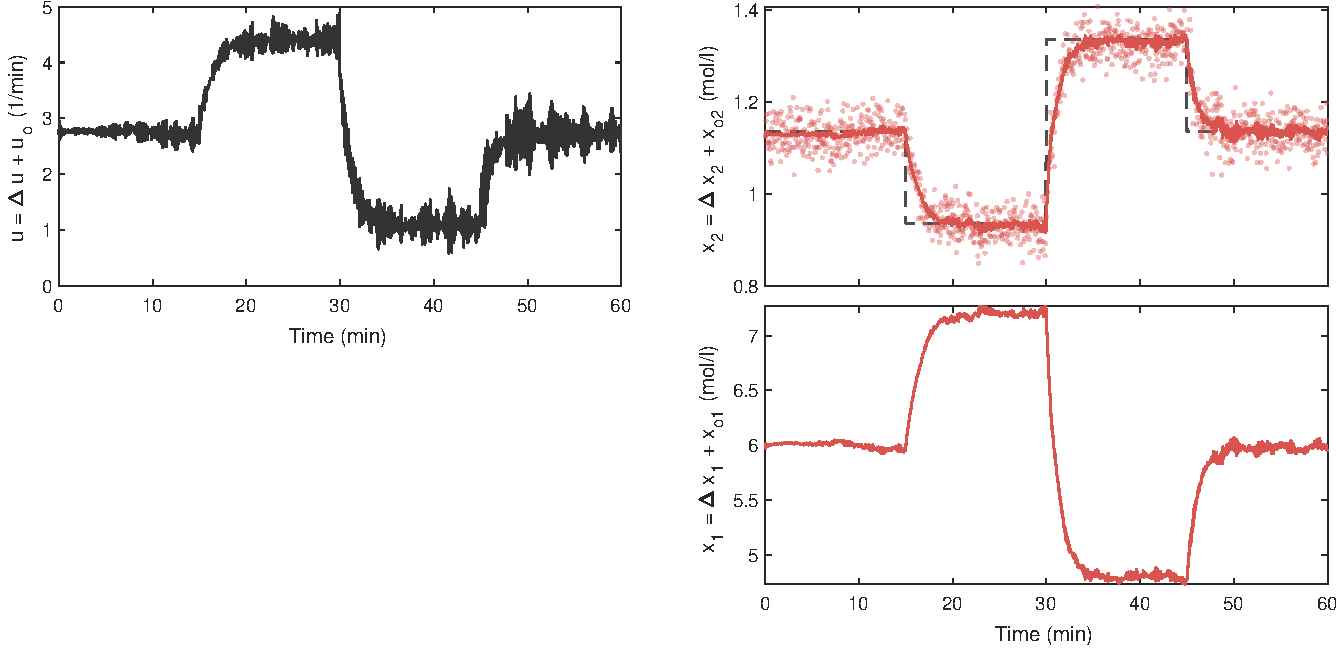
\includegraphics[width=0.9\textwidth]{chapter4/report_ch4_1}
	\caption{Simulation of the LQG controllers showing the input signal (left) and correspondent actual state responses (right). The dots denotes represents the measurements from the real system.}
	\label{fig:lqg02}
\end{figure}

\section{Stability and Robustness Analysis}

In the last chapter, the poles of the feedback controlled system where arbitrarily assigned using the pole-placement method. In this chapter, however, the controllers result from optimization procedures, so it is necessary to discuss whether or not these controllers are stable and robust given the criteria already presented. 

\subsubsection{Stability}

First of all, the stability of the closed-loop system via Linear Quadratic Regulator is discussed. One might conclude that, since this controller is obtained from an optimization process, the resulting controller can not be unstable. Consider, however, the popular counter-intuition: consider a scalar system $\dot{x}(t) = x(t) + u(t)$, with $R = 1$ and $Q = 0$, such that its associated LQR cost function is:
\begin{equation}
    J(x,u,t_0) = \int_{t_0}^{\infty} u^2(t) dt
.\end{equation}

In this case, the optimal control action is always $u(t) = 0$, for $t \in [t_0, \infty]$. However, this control action results in the system $\dot{x}(t) = x(t)$ which is clearly BIBO unstable. Therefore, there are conditions under which the optimization process may result in a stable or unstable closed-loop system, as shown by the following theorem.

\begin{boxed-theorem}{(LQR Assymptoptic Stability)} \label{th:lqrStab}
    Consider the infinite-horizon Linear Quadratic Regulator as defined in Theorem \ref{th:infiniteLQR}. If the system is observable, then the closed-loop matrix $\bm{A}_{cl} = (\bm{A} - \bm{B}\bm{K}) = (\bm{A} - \bm{B}\bm{R}^{-1}\bm{B}^T\bm{P})$ is BIBO stable.
\end{boxed-theorem}

\begin{proof}
    Consider, without loss of generality, that $\bm{Q} = \bm{C}^T \bm{C}$, which is still positive definite. In this case $\bm{C} = \bm{Q}^{1/2}$, given that $\bm{Q}^{1/2} \bm{Q}^{1/2} = \bm{C}$, which is a nonsingular matrix and the observability assumption holds. Furthermore, consider the LQR cost function given an optimal input trajectory $\bm{u}^* : \mathbb{R} \rightarrow \mathbb{R}^r$:
    \begin{equation} \label{eq:lqrStab01}
    J(\bm{x},\bm{u}^*,t_0) = \int_{t_0}^{\infty} \left( \bm{x}^T (\bm{C}^T \bm{C}) \bm{x} + (\bm{u}^*)^T \bm{R} \bm{u}^* \right) dt = \int_{t_0}^{\infty} \left( \bm{y}^T \bm{y} + (\bm{u}^*)^T \bm{R} \bm{u}^* \right) dt
.\end{equation}

The optimal output trajectory resulting from this control action is given by $\bm{y}^*(t) = \bm{C} \bm{x}^*(t)$, where $\bm{x}^*(t)$ is the corresponding optimal state trajectory. Since $\bm{u}^*(t)$ was obtained by solving the algebraic Riccati equation on Theorem \ref{th:infiniteLQR}, a well-known result is that the optimal cost function is bounded:
\begin{equation}
    \bm{V}^*(\bm{x}, t_0) \leq \bm{x}^T(t_0) \bm{P} \bm{x}(t_0)
,\end{equation}

\noindent and, therefore, \eqref{eq:lqrStab01} must also be bounded. This is only possible if $\bm{y}^*(t) \to 0$ and $\bm{u}^*(t) \to 0$ as $t \to \infty$, which, since the system is observable, directly implies $\bm{x}^*(t) \to 0$ as $t \to \infty$, concluding that the system is BIBO stable.
\end{proof}

Notice that, in contrast to the Pole-Placement method where the stability must be explicitly defined through the assignment of the eigenvalues, the LQR controller guarantees a stable closed-loop system directly, as long as the system is observable, even when the open-loop system is unstable. Since the BIBO stability (Definition \ref{def:BIBOStab}) discusses the magnitude of a system response as $t \to \infty$, the results are derived for infinite-horizon LQR. Despite of this, it is also possible to interpret some notion of stable response for finite-horizon LQR, since the cost function is always bounded by the optimal cost as conditioned by the Hamilton-Jacobi equation.

\subsubsection{Robustness}

Now, the discussion turns to the robustness properties of these optimal controllers. It can be shown that the LQR has a gain margin $GM = \infty$ and a phase margin $PM \geq \ang{60}$ \textbf{[reference]}. This assumption can be verified from a visual inspection of the Nyquist plot, as shown in Fig. \ref{fig:lqrProperties01}. The reason for these values comes from the fact that the Nyquist diagram of an optimal regulator never crosses the unit circle centered at $s = -1$ (implied by the Return Difference Equality). Therefore, the diagram never crosses the point $s = -1$ no matter how much the gain $K$ is changed, which establishes the infinite gain margin. In addition, the angle that the closest permissible point of an unit circle centered in $s = 0$ makes with the point $s = -1$ is exactly $\ang{60}$, which establishes the lower bound on the gain phase.

\begin{figure}[ht]
	\centering
	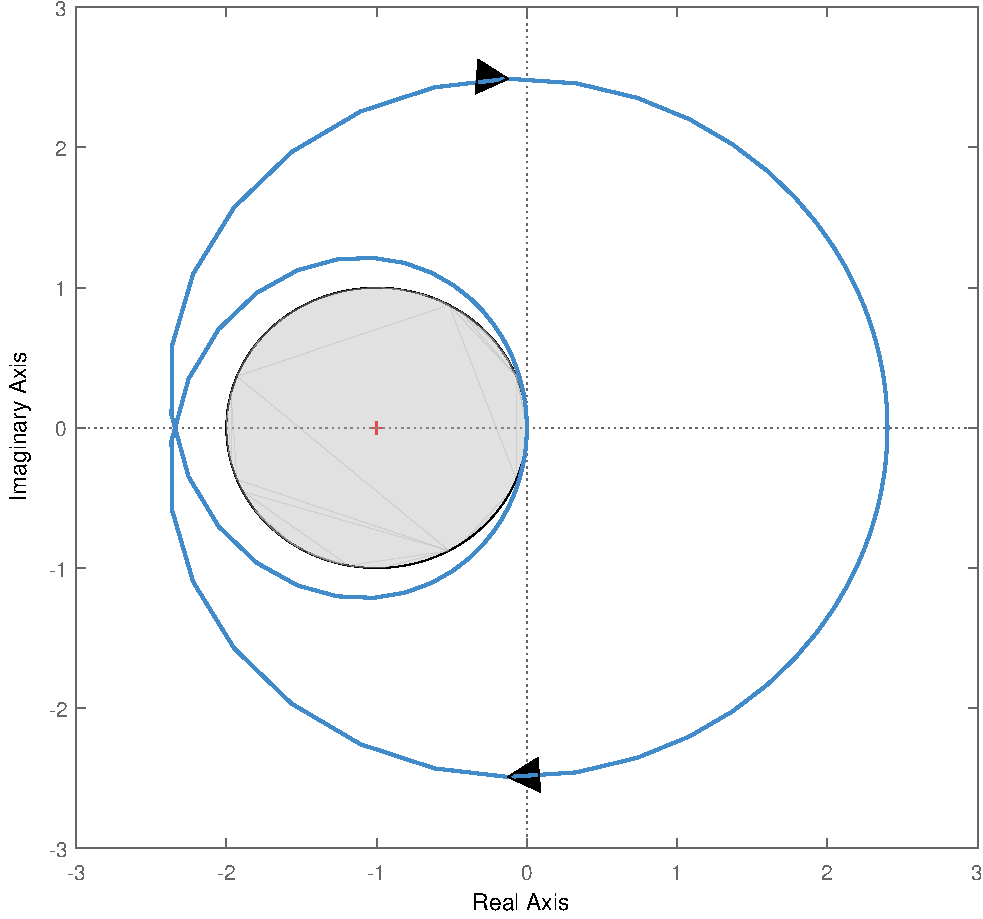
\includegraphics[scale=0.65]{chapter4/report_ch4_2}
	\caption{Nyquist diagram of a single state system with an open-loop unstable pole but which is closed-loop stable. The gain calculated by a LQR stabilizing controller never crosses the unit circle centered at $s = -1 + j0$.}
	\label{fig:lqrProperties01}
\end{figure}

Of course, there is no physical support of saying that a controller device exhibits an infinite gain margin, since there is always uncertainty about the model, the instrumentation and the environment. However, the fact that the mathematical model displays infinite gain margin allows for the assumption that the physical controller will have an extremely large margin. In fact, the uncertainty just mentioned is the main motivation into using optimal state estimators to reconstruct the state-vector from data, and it was shown by \textbf{[reference]} that an optimal controller-estimator configuration, i.e., the Linear Quadratic Gaussian, has no guaranteed margins.

%% 5 - Receding Horizon Optimal Control
%% ---------------------------------------------------------------
%\clearpage
%\chapter{Receding Horizon Optimal Control}
%
%The previous chapter introduced the concept of finite-horizon optimal control, presenting the Linear Quadratic Regulator as a solution to the condition imposed by the Hamilton-Jacobi equation. Despite being a popular solution with nice properties, there are some downsides of the LQR standard formulation. This chapter explores an optimal controller formulation based on a receding horizon control strategy. In the first section the motivation and definition of the moving horizon strategy are stated. The second sections explores the possibility of combining the receding horizon strategy with an iterative linearization procedure to yield an optimal operation in respect to the nonlinear system itself.
%
%\section{Optimization in Moving Horizons}
%
%A major disadvantage of the standard finite-horizon optimal controller is that the time in which the system will operate becomes restricted to the time horizon used for the optimization. This might becomes a problem in the case that the system is interrupted or subjected to strong disturbances, given that corrective action would require time and the desired state could not be achieved in the given horizon. Similarly, the restricted time horizon is also problematic in the case that the system should track a non-constant reference signal, since it also has be assumed of fixed length for the optimization to account for the entire signal. 
%
%A possible solution to this issue is to perform a Receding Horizon Control (RHC) strategy \textbf{[references]}. In the context of optimal control, a receding horizon controller is also known in literature as the \textit{Model-Predictive Controller} \textbf{[references]}, although this name is usually associated with constrained optimization procedures. The strategy is defined as follows:
%
%\begin{boxed-definition}{(Receding-Horizon Control)} \label{def:recedingHorizon}
%	Considers a linear system in State-Space form and a control horizon of size $T \in \mathbb{R}^+$. The \textit{Receding-Horizon Control} strategy for an optimal controller of this system is represented as:
%	\begin{equation}
%        \dot{\bm{x}}(t) = \left( \bm{A} - \bm{B} \bm{K}(t) \right) \bm{x}(t)
%    ,\end{equation} 
%    
%	\noindent where $\bm{K}(t) = - \bm{R}^{-1} \bm{B}^T \bm{P}(t)$ represents the optimal gain from the LQR cost function (Definition \ref{def:lqr}) for an iterative time interval $[t, t+T]$, and $\bm{P}(t)$ which solves the the Riccati differential equation:
%    \begin{equation}
%        -\dot{\bm{P}}(t) = \bm{A}^T \bm{P}(t) + \bm{P}(t) \bm{A} - \bm{P}(t) \bm{B} \bm{R}^{-1} \bm{B}^T \bm{P}(t) + \bm{Q}
%    ,\end{equation}
%    
%    \noindent with terminal condition $\bm{P}(t+T) = \bm{Q}_f$.
%\end{boxed-definition}
%
%In the optimization community, this problem is also popular in the following notation, where the moving horizon becomes explicit:
%\begin{align}
%\begin{matrix*}[l]
%    \textbf{minimize} & {\displaystyle \int_{t}^{t+T}  \left( \bm{x}^T \bm{Q} \bm{x} + \bm{u}^T \bm{R} \bm{u} \right) d\tau } \\
%    \hfill \textbf{s.t.} & \left. \begin{matrix*}[l] 
%    	\dot{\bm{x}}(\tau) = \bm{A}\bm{x}(\tau) + \bm{B}\bm{u}(\tau)  \\ 
%    	\bm{u}(\tau) = \pi(\bm{x}(t), \cdots, \bm{x}(\tau))
%    \end{matrix*} \right\} \forall \tau \in [t, t+T]
%\end{matrix*}
%.\end{align}
%
%This definition basically states that the optimization to be performed is similar to the standard case, but, since the time horizon is now a moving window of size $T$, the gain matrices $\bm{K} : \mathbb{R} \rightarrow \mathbb{R}^{r \times n}$ changes together with time. This is a consequence for the fact the the Ricatti differential equation has to be solved backwards in time for each new horizon at each new time instance. Of course, this means that for each which time interval that is optimized, only the first action is actually applied to the system. The Fig. \ref{fig:rhc01} illustrates this control strategy.
%
%\begin{figure}[ht]
%	\centering
%	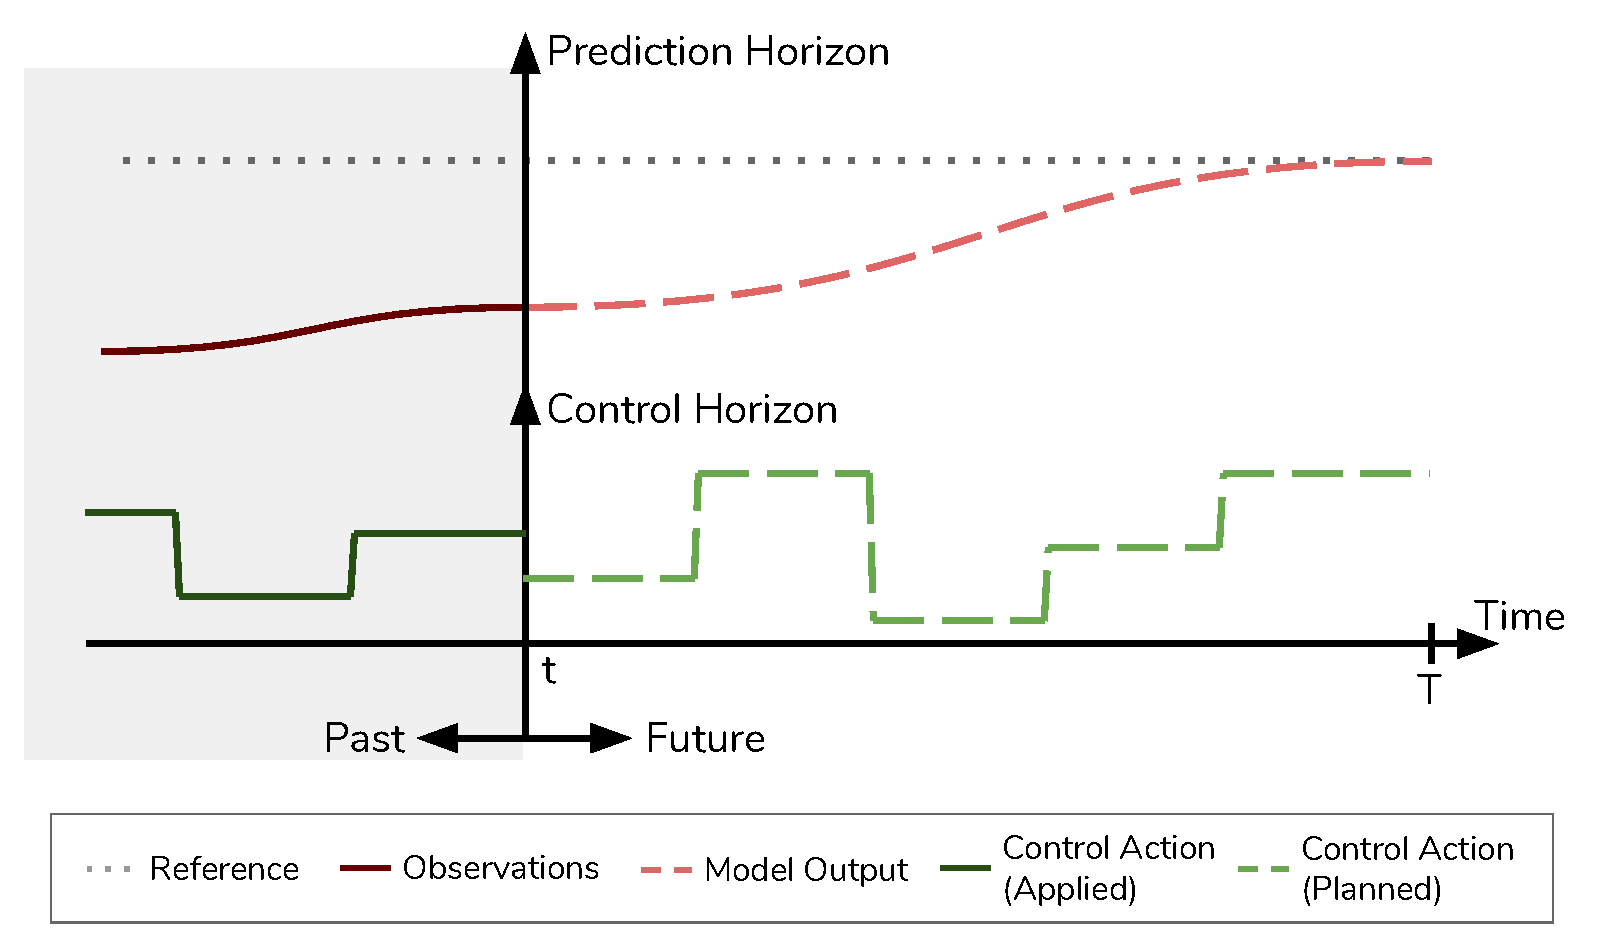
\includegraphics[width=\textwidth]{chapter5/recedingHorizon}
%	\caption{Illustration of the Receding Horizon Control strategy.}
%	\label{fig:rhc01}
%\end{figure}
%
%From the Separation Principle, it is always possible to increment this approach by introducing an optimal state estimator in a receding horizon fashion, as well. In this case, similarly to the controller, the optimal estimator gains are obtained for the entire horizon, but only the first gain is used to correct the state, before the horizon is updated.
%
%\textbf{[properties?]}
%
%\section{Linear Parameter-Varying Models}
%
%The optimal controllers discussed so far suffers from a performance disadvantage when regarding the control of nonlinear systems. As shown in Theorem \ref{th:linearization}, a nonlinear system can be approximated by a linear model around a specific steady-state point. The problem, however, is that the optimization accounts for a nominal linear system that, in the case of a linearized model, will not represent the real dynamics of the nonlinear system as its states deviates from the steady-state value used. For this reason, the LQR solution will not provide an optimal solution in the light of the real system.
%
%In this section, a solution to the nonlinear problematic is presented through an iterative linearization process, where the full dynamics are approximated by a series of linear models obtained for each time instance. This approach is referred in literature as Linear Switched Systems \textbf{[references]}. Before any further discussion, first consider the following definition.
%
%\begin{boxed-definition}{(Linear Parameter-Varying System)} \label{def:lpv}
%	A \textit{Linear Parameter-Varying} (LPV) State-Space representation describing a system with state vector $\bm{x} : \mathbb{R} \rightarrow \mathbb{R}^{n}$, output vector $\bm{y} : \mathbb{R} \rightarrow \mathbb{R}^{p}$ and input vector $\bm{u} : \mathbb{R} \rightarrow \mathbb{R}^{r}$ is given by the system of equations: 
%    \begin{align} \label{eq:SSRepr04}
%    \begin{cases}
%        \dot{\bm{x}}(t) = \bm{A}(\bm{\theta}(t)) \bm{x}(t) + \bm{B}(\bm{\theta}(t)) \bm{u}(t) & \\
%        \bm{y}(t) = \bm{C}(\bm{\theta}(t)) \bm{x}(t) + \bm{D}(\bm{\theta}(t)) \bm{u}(t) &
%    \end{cases}
%    ,\end{align}
%
%    \noindent where $\bm{A}(\cdot) \in \mathbb{R}^{n \times n}$, $\bm{B}(\cdot) \in \mathbb{R}^{n \times r}$, $\bm{C}(\cdot) \in \mathbb{R}^{p \times n}$ and $\bm{D}(\cdot) \in \mathbb{R}^{p \times r}$ are appropriate functions of the parameter function $\bm{\theta} : \mathbb{R} \rightarrow \mathbb{R}^{z}$. 
%\end{boxed-definition}
%
%The LPV State-Space model is a linear realization of a system that can change with time through the result of a function $\bm{\theta}(\cdot)$. The first discussions on this representation for dynamical models were motivated from the Gain Scheduling control method \textbf{[references]}, where it serves as an linear embedding of the nonlinear model. From Theorem \ref{th:linearization} it is clear that a possible formulation for such a model is given by: 
%\begin{equation}
%\begin{cases}
%        \Delta \dot{\bm{x}}(t)) =\left. \cfrac{\partial \bm{f}}{\partial \bm{x}}\right\vert_{\bm{x}_o, \bm{u}_o} \Delta \bm{x}(t) + \left. \cfrac{\partial \bm{f}}{\partial \bm{u}}\right\vert_{\bm{x}_o,  \bm{u}_o}  \Delta \bm{u}(t) \\ \\
%        \hfill \bm{y}(t) = \left. \cfrac{\partial \bm{g}}{\partial \bm{x}}\right\vert_{\bm{x}_o, \bm{u}_o} \Delta \bm{x}(t) + \left. \cfrac{\partial \bm{g}}{\partial \bm{u}}\right\vert_{\bm{x}_o, \bm{u}_o} \Delta \bm{u}(t) \\
%\end{cases}
%,\end{equation}
%
%\noindent in which case it is possible to set $\bm{\theta}(t) = \begin{bmatrix} \bm{x}(t-\delta t), \bm{u}(t-\delta t) \end{bmatrix}^T$ and denote the Jacobians as:
%\begin{align} \label{eq:lpvJacobians}
%\begin{matrix*}[l]
%        \bm{A}(\bm{x}(t-\delta t), \bm{u}(t-\delta t)) = \left. \cfrac{\partial \bm{f}}{\partial \bm{x}}\right\vert_{\bm{x}(t-\delta t), \bm{u}(t-\delta t)}; & \bm{B}(\bm{x}(t-\delta t), \bm{u}(t-\delta t)) = \left. \cfrac{\partial \bm{f}}{\partial \bm{u}}\right\vert_{\bm{x}(t-\delta t), \bm{u}(t-\delta t)}; \\ \\ \bm{C}(\bm{x}(t-\delta t), \bm{u}(t-\delta t)) = \left. \cfrac{\partial \bm{g}}{\partial \bm{x}}\right\vert_{\bm{x}(t-\delta t), \bm{u}(t-\delta t)} ; & \bm{D}(\bm{x}(t-\delta t), \bm{u}(t-\delta t)) = \left. \cfrac{\partial \bm{g}}{\partial \bm{u}}\right\vert_{\bm{x}(t-\delta t), \bm{u}(t-\delta t)} 
%\end{matrix*}
%\end{align}
%
%The formulation in \eqref{eq:lpvJacobians} might not be a perfect linearization of the system, since the values $\bm{x}(t)$ and $\bm{u}(t)$ are not constrained to yield $\bm{f}(\bm{x}(t), \bm{u}(t))$, i.e., they may be non-stationary points of the system. In the case that $\delta t > 0$, these matrices functions represents a causal switching law for linear systems \textbf{[reference]}, and the LPV system tends to a nonlinear system as $\delta t \to 0$. For some families of state and input trajectories it is possible to guarantee stability and other asymptotic system properties \textbf{[reference]}, which are heavily based on Lyapunov's theory \textbf{[reference]}. 
%
%Consider the linearization Jacobians stated in \eqref{eq:isoReact01}. In the case that only the two first states are modelled, a LPV formulation for that system is given as:
%\begin{align}   \label{eq:isoReactLPV}
%\left\{ \begin{matrix*}[l]
%    \Delta \dot{\bm{x}}(t) = \begin{bmatrix}
%        -\theta^{(1)} - K_{AB} - 2K_{AC} \bm{\theta}^{(2)}_1 & 0 \\ K_{AB} & - \theta^{(1)} - K_{BC} 
%    \end{bmatrix} \Delta \bm{x}(t) +  \begin{bmatrix}
%        \rho_{in}^{(A)} - \bm{\theta}^{(2)}_1 \\ - \bm{\theta}^{(2)}_2
%    \end{bmatrix} \Delta u(t) \\ \\
%    \phantom{\Delta} \bm{y}(t) = \begin{bmatrix}
%        1 & 0  \\ 0 & 1 
%    \end{bmatrix} \Delta \bm{x}(t) + \begin{bmatrix}
%        0 \\ 0 
%    \end{bmatrix} \Delta u(t)
%\end{matrix*} \right.
%,\end{align}
%
%\noindent where $\theta^{(1)} = u(t-\delta t)$ and $\bm{\theta}^{(2)} = \bm{x}(t-\delta t)$. Notice that the matrix $\bm{A}(\cdot)$ in this case should always result in a stable system, since the variables in the diagonal are constrained to be positive, given their physical meaning. A simulation is shown in Fig. \ref{fig:lpvSim01} for this system, given a sequence of different amplitude steps as inputs, to visualize how well this system response can approxima	te the nonlinear response.
%
%[fig]
%
%\section{Receding Horizon Control for Switched Systems}
%
%Combining the receding horizon strategy together with the linear switching approach, it is possible to develop a method to controlling nonlinear systems by optimizing over a series of linearized systems. The receding horizon, in this case, becomes a necessity since the optimization has to be repeated every time that the matrices $\bm{A}(\cdot)$ and $\bm{B}(\cdot)$ changes. A formal definition of such controller is given below.
%
%\begin{boxed-definition}{(RHC for LPV Systems)} \label{def:recedingHorizon}
%	Considers a linear parameter-varying system in State-Space form, a control horizon of size $T \in \mathbb{R}^+$ and a switching time distance $\delta t$. The receding horizon control strategy for an optimal controller of this switched system is represented as:
%	\begin{equation}
%        \dot{\bm{x}}(t) = \left( \bm{A}(\bm{\theta}(t)) - \bm{B}(\bm{\theta}(t)) \bm{K}(t) \right) \bm{x}(t)
%    ,\end{equation} 
%    
%	\noindent where $\bm{\theta}(t) = \begin{bmatrix} \bm{x}(t - \delta t), \bm{u}(t - \delta t) \end{bmatrix}$ is the parameter function and $\bm{K}(t) = - \bm{R}^{-1} \bm{B}^T(\bm{\theta}(t)) \bm{P}(t)$ represents the optimal gain for an iterative time interval $[t, t+T]$, given $\bm{P}(t)$ which solves the the Riccati differential equation:
%    \begin{equation}
%        -\dot{\bm{P}}(t) = \bm{A}^T(\bm{\theta}(t)) \bm{P}(t) + \bm{P}(t) \bm{A}(\bm{\theta}(t)) - \bm{P}(t) \bm{B}(\bm{\theta}(t)) \bm{R}^{-1} \bm{B}^T(\bm{\theta}(t)) \bm{P}(t) + \bm{Q}
%    ,\end{equation}
%    
%    \noindent with terminal condition $\bm{P}(t+T) = \bm{Q}_f$.
%\end{boxed-definition}
%
%A simulation of controlling the system from \eqref{eq:isoReactLPV} is shown at Fig. \ref{fig:rhcLPV01}, demonstrating the quality of this approach to directly control the nonlinear system. For this configuration, the transient characteristics of the response can then be tuned by the design of $\bm{Q}$, $\bm{R}$ and the time parameters $\bm{T}$ and $\delta t$. 
%
%[fig]
%
%As stated earlier, it is also possible to apply this approach to stochastic systems, which are modelled as the nominal State-Space models perturbed by white Gaussian noise. The main difference is that the switching is done through the estimated states, making the approximation to the nonlinear response dependent on the estimator capabilities. A simulation of such configuration is shown in Fig. \ref{fig:rhcLPV02}. Notice how the action of noise made the closed-loop system exhibits some pseudo-periodic behavior, while still being able to follow the reference signal.
%
%[fig]

% 6 - Methodology
% ---------------------------------------------------------------
\clearpage
\chapter{Methodology}

This chapter details the methodology used in order to attest the discussion presented until now. The experiments were performed in a simulated environment, using the MATLAB software \textbf{[reference]} as the framework to compute such simulations. The results obtained are presented and discussed in the next chapter.   

\section{Non-Isothermal Continuous Stirred Tank}

The system used for the experiments was the non-isothermal Continuous Stirred Tank Reactor (CSTR) presented by \textbf{[reference-Engel]}. This system is a realization of a class of processes that characterize a wide range of industrial applications, hence being considered a classical benchmark for reactor systems. In particular, the system proposed for the experiment is a multiple-input multiple-output (MIMO) system which is highly nonlinear, with non-minimum phase behavior and unmeasurable states, thus makes it very challenging to control \textbf{[reference]}. 

This system is comprised by a tank containing a dilute solution of cyclopentadiene ($\textbf{C}_5 \textbf{H}_6$), which suffers reactions together with water molecules and together with the side-products of these reactions. The reaction scheme follows the same Van de Vusse scheme explored earlier in this report:
\begin{align}
\left\{\ \begin{matrix*}[l]
	\overbrace{\textbf{C}_5 \textbf{H}_6}^{A} & \overset{K_1(T)}{\longrightarrow} & \overbrace{\textbf{C}_5 \textbf{H}_7 \textbf{OH}}^{B} & \overset{K_2(T)}{\longrightarrow} & \overbrace{\textbf{C}_5 \textbf{H}_8 \textbf{(OH)}_2}^{C} \\ 
	\overbrace{2 \textbf{C}_5 \textbf{H}_6}^{2A} & \overset{K_3(T)}{\longrightarrow} & \overbrace{\textbf{C}_10 \textbf{H}_12}^{D}
\end{matrix*} \right.
.\end{align}

Since the reaction is non-isothermal, the kinetics rates $K_1(T)$, $K_2(T)$ and $K_3(T)$ are function of the temperature inside the tank, and they are assumed to follow the Arrhenius equation in the form:
\begin{equation}
	K_{i}(T) = K_{i0} e^{\frac{-E_i / R}{T+273.15}}
\end{equation}

In order to control the temperature, ensuring some safety constraints to the process, a coolant system is coupled to the tank reactor to perform heat exchange by conduction. This scenario also assumes that only the concentration of chemical $\textbf{C}_5 \textbf{H}_7 \textbf{OH}$ and the temperature inside the tank can be measured. Additionally, the liquid inflow into the tank carries only the chemical $\textbf{C}_5 \textbf{H}_6$ with a concentration $\rho^{(A)}_{in}$ and temperature $T_{in}$. The schematic of this operation is shown in Fig. \ref{fig:methodology01}. 

\begin{figure}[ht] \centering
	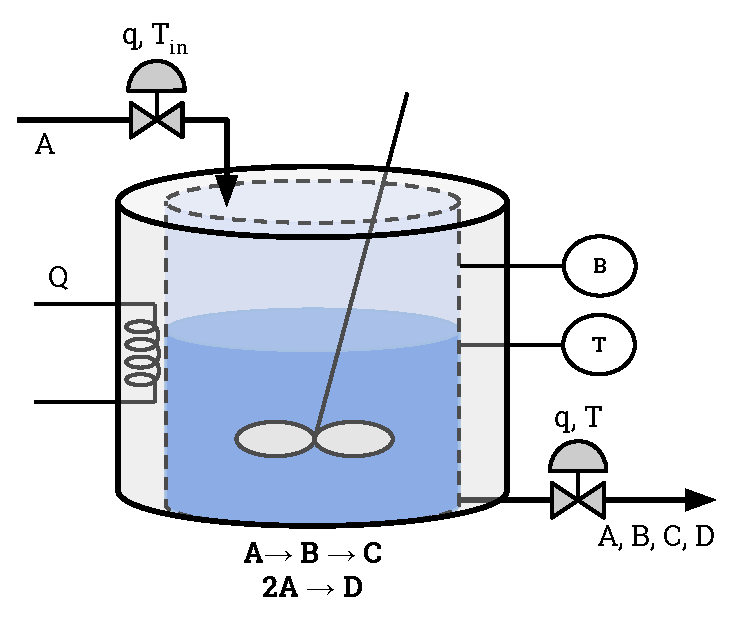
\includegraphics[scale=0.75]{chapter6/exoCSTR}
	\caption{The non-isothermal continuous stirred tank reactor proposed.}
	\label{fig:methodology01}
\end{figure}

A nonlinear dynamical model, which was obtained from the first principles approach, is proposed to represent the evolution of the important states:
\begin{align} \label{eq:engellModel}
\begin{cases}
	\hfill \cfrac{d \rho_A}{dt} &= q (\rho^{(A)}_{in} - \rho_A) - \left( K_1(T) \rho_A + K_3(T) \rho^2_A  \right) \\
	\hfill \cfrac{d \rho_B}{dt} &= - q \rho_B + K_1(T) \rho_A - K_2(T) \rho_B \\
	\hfill \cfrac{d T}{dt} &= q(T_{in} - T) + \cfrac{k_W A_r}{\varrho C_p V_r} (T_C - T) \\ & \ \ \ \ \ \ \ \ \ \ \ \ -\cfrac{1}{\varrho C_p} \left( K_1(T) \rho_A \Delta H_{AB} + K_2(T) \rho_B \Delta H_{BC} + K_1(T) \rho_A^2 \Delta H_{AC} \right) \\
	\hfill \cfrac{d T_C}{dt} &= \cfrac{1}{m_K C_{pK}} Q + \cfrac{k_W A_r}{m_K C_{pK}} (T - T_C) 
\end{cases}
.\end{align}

The meaning and value of each system variable is shown in Table \ref{table:exo_parameters}. Additionally, the real system has some constraints in respect to the manipulated variables, namely:
\begin{equation}
\begin{matrix}
	5 hr^{-1} \leq F \leq 35 h^{-1}; & -8500 \cfrac{kJ}{h} \leq Q \leq 0 \cfrac{kJ}{h}
\end{matrix}
.\end{equation}

\begin{table}[ht]
  \centering
	\begin{tabular}{l | c | c l }
	\textbf{System Variable} & \textbf{Symbol} & \textbf{Value} & \textbf{Unit} \\
	\hline
	Concentration $A$ in the reactor solution & $\rho_A$ 	& $-$		& $\text{mol}/l$ \\
	Concentration $A$ in the reactor solution & $\rho_B$ 	& $-$		& $\text{mol}/l$ \\
	Temperature inside the reactor & $T$ 	& $-$		& $º C$ \\
	Temperature of the coolant jacket & $T_C$ 	& $-$		& $º C$ \\
	\hline
	Inflow concentration of $A$ & $\rho^{(A)}_{in}$ 	& $5.1$		& $\text{mol}/l$ \\
	Inflow liquid temperature & $T_{in}$ 	& $130$		& $º C$ \\
	Nominal kinetic rate for $A \rightarrow B$ & $K_{10}$	& $(1.287)\times 10^{12}$	& $h^{-1}$ \\
	Nominal kinetic rate for $B \rightarrow D$ & $K_{20}$	& $(1.287)\times 10^{12}$	& $h^{-1}$ \\
	Nominal kinetic rate for $2A \rightarrow D$ & $K_{30}$	& $(9.043)\times 10^{9}$	& $l\  \text{mol}^{-1} h $ \\
	Activation energy for $A \rightarrow B$ & $E_{1}/R$	& $9758.3$	& - \\
	Activation energy for $B \rightarrow C$ & $E_{2}/R$	& $9758.3$	& - \\
	Activation energy for $2A \rightarrow D$ & $E_{3}/R$	& $8560.0$	& - \\
	Enthalpy for $A \rightarrow B$ & $\Delta H_{AB}$	& $4.2$	& $kJ/mol$ \\
	Enthalpy for $B \rightarrow C$ & $\Delta H_{BC}$	& $-11.0$	& $kJ/mol$ \\
	Enthalpy for $2A \rightarrow D$ & $\Delta H_{AD}$	& $-41.85$	& $kJ/mol$ \\
	Total density of the reactor solution & $\varrho$ & $(0.9342)\times 10^{-4}$ & $kg/l$ \\
	Heat capacity of the solution & $C_p$ & $3.01$ & $kJ\ kg^{-1} K$ \\
	Heat capacity of the coolant & $C_{pK}$ & $2.0$ & $kJ\ kg^{-1} K^{-1}$ \\
	Surface area of the tank reactor & $A_R$ & $0.215$ & $m^2$ \\
	Volume of the tank reactor & $V_R$ & $10.01$ & $m^3$ \\
	Coolant mass & $m_K$ & $5.0$ & $kg$ \\
	Heat transfer coefficient & $k_W$ & $4032.0$ & $kJ\ h^{-1} m^2 K$ \\
  \end{tabular} 
  \caption{Model parameters and variables nomenclature.}
  \label{table:exo_parameters} 
\end{table} \vskip0.25cm


\section{Simulation}

The process and all the control structures were simulated using the MATLAB software. In the first part of the experiments, the dynamics of the process were analyzed in respect to the mathematical structure of the models and through the simulation results. 

In respect to the control, the second part of the experiments focused on the design of controllers using the optimal control techniques. The controllers were developed and analyzed in the same order that they were presented in this document:
\begin{enumerate}
	\item Linear Quadratic Regulator, assuming a nonzero initial state and perfect measurement of the states;
	\item Linear Quadratic Regulator with Integral Action, for a non-constant reference signals and assuming perfect measurement of the states;
	\item Linear Quadratic Gaussian, assuming a nonzero initial state and reconstruction of the state-vector through observations from a stochastic linear system;
	\item Linear Quadratic Gaussian with Integral Action, for a non-constant reference and assuming a reconstruction of the state-vector through observations from a stochastic linear system;
\end{enumerate}

The simulation results are mainly analyzed through graphical visualizations of the data obtained. The experiments were focused on validating the modeling and control procedures for the system presented, instead of comparing and ranking the controllers based on the most performing one. For the sake of completeness, however, some metrics are used to evaluate each controller performance and relate them to the visualizations. The metrics used were the \textit{Integral of Squared Error} (ISE), \textit{Integral of Absolute Error} (IAE), \textit{Integral of Time-Weighted Squared Error} (ITSE) and \textit{Integral of Time-Weighted Absolute Error} (ITAE), which are given as:
\begin{align}
\begin{matrix*}[l] \displaystyle
	\text{IAE} = \displaystyle\int_{t_0}^{T} | \bm{r}(\tau) - \bm{y}(\tau) | d\tau; & & \text{ITAE} = \displaystyle\int_{t_0}^{T} \tau | \bm{r}(\tau) - \bm{y}(\tau) | d\tau;\\ \\
	\text{ISE} = \displaystyle\int_{t_0}^{T} \left[ \bm{r}(\tau) - \bm{y}(\tau) \right]^2 d\tau; & & \text{ITSE} = \displaystyle\int_{t_0}^{T} \tau \left[ \bm{r}(\tau) - \bm{y}(\tau) \right]^2 d\tau.
\end{matrix*}
\end{align}


% 7 - Results and Discussion
% ---------------------------------------------------------------
\clearpage
\chapter{Results and Discussion}

a

\section{Dynamical Analysis}

\subsection{Nonlinear model simulation}

The behavior of the process is accessed directly by simulating the nonlinear model presented at \eqref{eq:engellModel}. The main goal is to observe how the system responds to variations in each of its manipulated variables. In the first simulation, shown in Fig. \ref{fig:dynamics01}, the process is started at the steady-state condition, and then a pulse is applied to the liquid inflow to the tank. The response in each system is shown at the right side of the figure, where the states relating concentrations and the ones relating temperatures are grouped in different plots. The dashed lines represents the response of for compounds $C$ and $D$, which are not given by the proposed model, but can easily be equated following the first-principles approach.

\begin{figure}[ht] \centering
	\begin{tikzpicture}	[node distance=0.7cm]
		\node (plot) {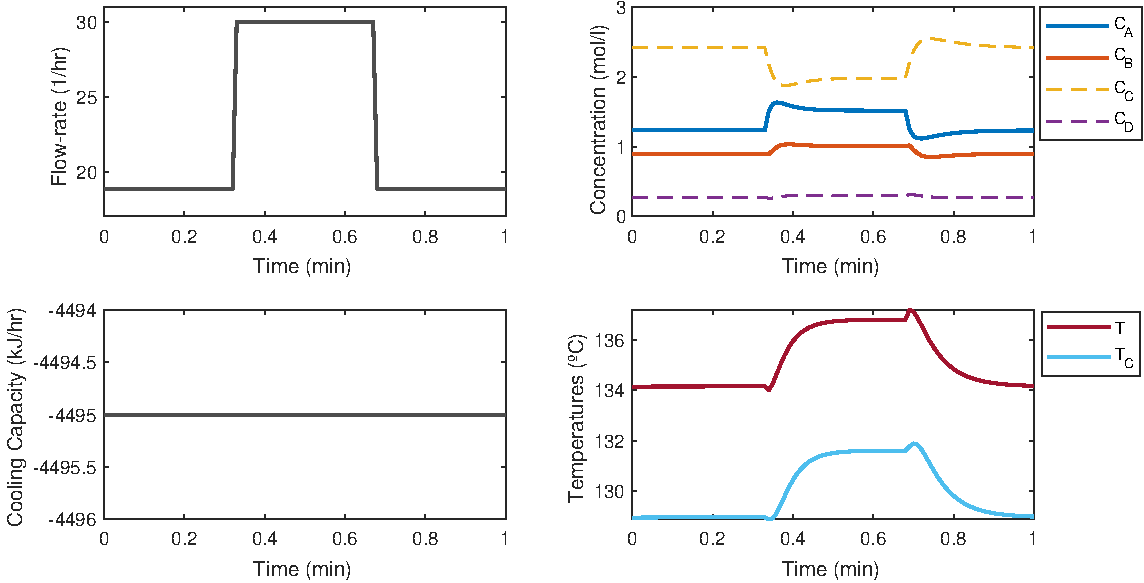
\includegraphics[width=\textwidth]{chapter7/dynamics01}};
		
		\begin{scope}[on background layer]
			\node[block, above of=plot, xshift=0.65cm, node distance=5cm, minimum width=0.91\textwidth] (legendBox) {};
		\end{scope}
		
		\definecolor{linecolor}{rgb}{0, 0.4470, 0.7410};
		\node at (legendBox.west) [xshift=0.6cm]  (legendStart) {};
		\node[right of=legendStart, node distance=1.5cm] (label) {$\rho_A$};		
		\draw[-, linecolor, line width=1.5pt] (legendStart) -- (label);
		
		\definecolor{linecolor}{rgb}{0.8500,0.3250,0.0980};
		\node[right of=label]  (legendStart) {};
		\node[right of=legendStart, node distance=1.5cm] (label) {$\rho_B$};		
		\draw[-, linecolor, line width=1.5pt] (legendStart) -- (label);
		
		\definecolor{linecolor}{rgb}{0.9290, 0.6940, 0.1250};
		\node[right of=label]  (legendStart) {};
		\node[right of=legendStart, node distance=1.5cm] (label) {$\rho_C$};		
		\draw[-, dashed, linecolor, line width=1.5pt] (legendStart) -- (label);
		
		\definecolor{linecolor}{rgb}{0.4940, 0.1840, 0.5560};
		\node[right of=label]  (legendStart) {};
		\node[right of=legendStart, node distance=1.5cm] (label) {$\rho_D$};		
		\draw[-, dashed, linecolor, line width=1.5pt] (legendStart) -- (label);
		
		\definecolor{linecolor}{rgb}{0.6350, 0.0780, 0.1840};
		\node[right of=label]  (legendStart) {};
		\node[right of=legendStart, node distance=1.5cm] (label) {$T$};		
		\draw[-, linecolor, line width=1.5pt] (legendStart) -- (label);
		
		\definecolor{linecolor}{rgb}{0.3010, 0.7450, 0.9330};
		\node[right of=label]  (legendStart) {};
		\node[right of=legendStart, node distance=1.5cm] (label) {$T_c$};		
		\draw[-, linecolor, line width=1.5pt] (legendStart) -- (label);
	\end{tikzpicture}	

	\caption{Non-linear simulation showing the manipulated variables (left) and correspondent response of the system variables (right) for a pulse change in the input flow-rate.}
	\label{fig:dynamics01}
\end{figure}

The simulation shows that both compounds $A$ and $B$ grows together when there is an increase in the input flow-rate, in which case the first exhibits a greater response than the other. Of course, this conclusion is direct from the fact that the input carries concentrations of this very same chemical. In respect to the temperatures, notice that, since the process is non-isothermal, the temperatures raised together with the increase in the reagents concentrations. Given that the temperature of the liquid inflow is actually lower than the tank temperature at the steady-state, it is possible to relate the increase in the temperature directly to the occurrence of the chemical reactions. This fact characterizes the process as an exothermic process, as it can be also noted from the first-principles model.

The second simulation was performed similarly, but applying a negative pulse to the jacket cooling capacity. The result is shown in Fig. \ref{fig:dynamics02}. As expected, the change in the cooling capacity affects the temperatures inside the reactor tank and inside the cooling jacket. The visualization also shows that the change in the temperature slightly changed the concentration of the substances inside the reactor. Therefore, it is possible to consider an indirect effect of this manipulated variable to these system variables.

\begin{figure}[ht] \centering
		\begin{tikzpicture}	[node distance=0.7cm]
		\node (plot) {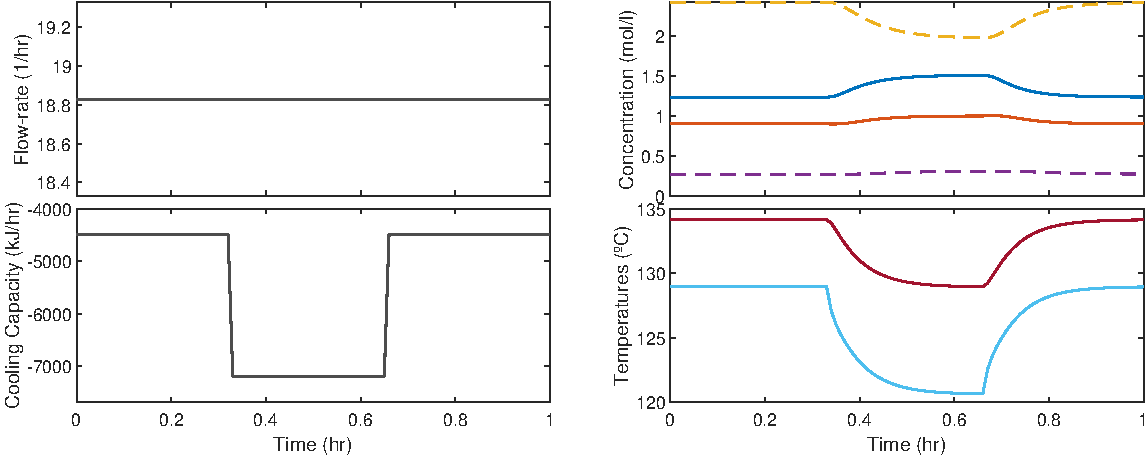
\includegraphics[width=\textwidth]{chapter7/dynamics02}};
		
		\begin{scope}[on background layer]
			\node[block, above of=plot, xshift=0.65cm, node distance=5cm, minimum width=0.91\textwidth] (legendBox) {};
		\end{scope}
		
		\definecolor{linecolor}{rgb}{0, 0.4470, 0.7410};
		\node at (legendBox.west) [xshift=0.6cm]  (legendStart) {};
		\node[right of=legendStart, node distance=1.5cm] (label) {$\rho_A$};		
		\draw[-, linecolor, line width=1.5pt] (legendStart) -- (label);
		
		\definecolor{linecolor}{rgb}{0.8500,0.3250,0.0980};
		\node[right of=label]  (legendStart) {};
		\node[right of=legendStart, node distance=1.5cm] (label) {$\rho_B$};		
		\draw[-, linecolor, line width=1.5pt] (legendStart) -- (label);
		
		\definecolor{linecolor}{rgb}{0.9290, 0.6940, 0.1250};
		\node[right of=label]  (legendStart) {};
		\node[right of=legendStart, node distance=1.5cm] (label) {$\rho_C$};		
		\draw[-, dashed, linecolor, line width=1.5pt] (legendStart) -- (label);
		
		\definecolor{linecolor}{rgb}{0.4940, 0.1840, 0.5560};
		\node[right of=label]  (legendStart) {};
		\node[right of=legendStart, node distance=1.5cm] (label) {$\rho_D$};		
		\draw[-, dashed, linecolor, line width=1.5pt] (legendStart) -- (label);
		
		\definecolor{linecolor}{rgb}{0.6350, 0.0780, 0.1840};
		\node[right of=label]  (legendStart) {};
		\node[right of=legendStart, node distance=1.5cm] (label) {$T$};		
		\draw[-, linecolor, line width=1.5pt] (legendStart) -- (label);
		
		\definecolor{linecolor}{rgb}{0.3010, 0.7450, 0.9330};
		\node[right of=label]  (legendStart) {};
		\node[right of=legendStart, node distance=1.5cm] (label) {$T_c$};		
		\draw[-, linecolor, line width=1.5pt] (legendStart) -- (label);
	\end{tikzpicture}	
	
	\caption{Non-linear simulation showing the manipulated variables (left) and correspondent response of the system variables (right) for a pulse change in the cooling capacity.}
	\label{fig:dynamics02}
\end{figure}

Now, the goal was to visualize if it is possible to increase the concentration of the chemicals through the reactions, while maintaining the tank temperature close to the steady-state value. For this reason, the last simulation considers a pulse to increase the input flow-rate while another pulse increases the magnitude of the cooling capacity. The result of this simulation is shown at Fig. \ref{fig:dynamics03}. Note that the tank temperature remained restricted to values closer to the steady-state point, whereas the concentrations were increased by the flow-rate input. Therefore, the possibility of increasing the production of a chemical without breaking safety constraints holds.

\begin{figure}[ht] \centering
		\begin{tikzpicture}	[node distance=0.7cm]
		\node (plot) {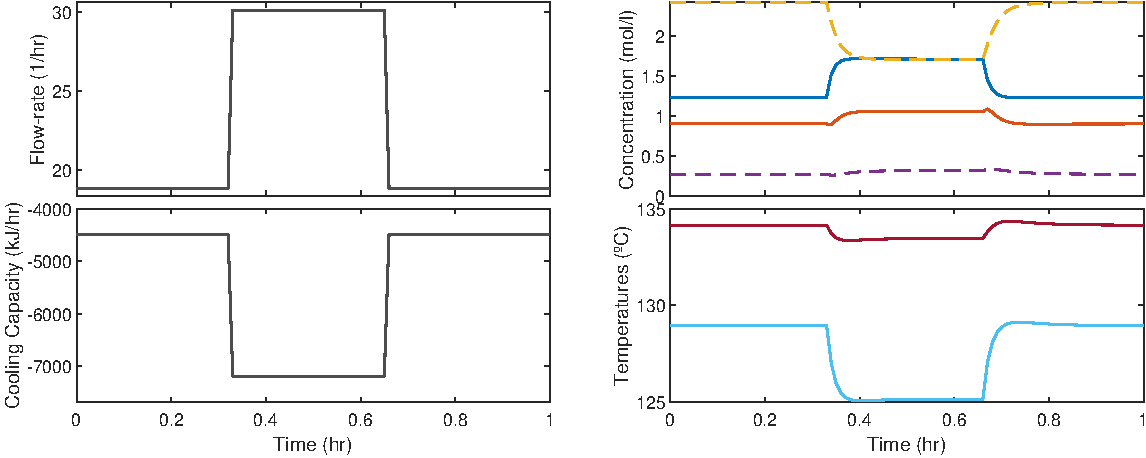
\includegraphics[width=\textwidth]{chapter7/dynamics03}};
		
		\begin{scope}[on background layer]
			\node[block, above of=plot, xshift=0.65cm, node distance=5cm, minimum width=0.91\textwidth] (legendBox) {};
		\end{scope}
		
		\definecolor{linecolor}{rgb}{0, 0.4470, 0.7410};
		\node at (legendBox.west) [xshift=0.6cm]  (legendStart) {};
		\node[right of=legendStart, node distance=1.5cm] (label) {$\rho_A$};		
		\draw[-, linecolor, line width=1.5pt] (legendStart) -- (label);
		
		\definecolor{linecolor}{rgb}{0.8500,0.3250,0.0980};
		\node[right of=label]  (legendStart) {};
		\node[right of=legendStart, node distance=1.5cm] (label) {$\rho_B$};		
		\draw[-, linecolor, line width=1.5pt] (legendStart) -- (label);
		
		\definecolor{linecolor}{rgb}{0.9290, 0.6940, 0.1250};
		\node[right of=label]  (legendStart) {};
		\node[right of=legendStart, node distance=1.5cm] (label) {$\rho_C$};		
		\draw[-, dashed, linecolor, line width=1.5pt] (legendStart) -- (label);
		
		\definecolor{linecolor}{rgb}{0.4940, 0.1840, 0.5560};
		\node[right of=label]  (legendStart) {};
		\node[right of=legendStart, node distance=1.5cm] (label) {$\rho_D$};		
		\draw[-, dashed, linecolor, line width=1.5pt] (legendStart) -- (label);
		
		\definecolor{linecolor}{rgb}{0.6350, 0.0780, 0.1840};
		\node[right of=label]  (legendStart) {};
		\node[right of=legendStart, node distance=1.5cm] (label) {$T$};		
		\draw[-, linecolor, line width=1.5pt] (legendStart) -- (label);
		
		\definecolor{linecolor}{rgb}{0.3010, 0.7450, 0.9330};
		\node[right of=label]  (legendStart) {};
		\node[right of=legendStart, node distance=1.5cm] (label) {$T_c$};		
		\draw[-, linecolor, line width=1.5pt] (legendStart) -- (label);
	\end{tikzpicture}	
	
	\caption{Non-linear simulation showing the manipulated variables (left) and correspondent response of the system variables (right) for a change in the input flow-rate and cooling capacity.}
	\label{fig:dynamics03}
\end{figure}

\subsection{Linearized model realization and simulation}

The discussion throughout the document focused on control design methods for linear systems. For this reason, the nonlinear model can not directly be used to develop the controllers, and a linearization (Theorem \ref{th:linearization}) of this model is required. First of all, consider the following choice for the state, input and output variables:
\begin{equation}
\begin{matrix}
	\bm{x}(t) = \begin{bmatrix}
		\rho_A(t) \\ 
		\rho_B(t) \\ 
		T(t) \\ 
		T_c(t)
	\end{bmatrix}; & \bm{u}(t) = \begin{bmatrix}
		q(t) \\ 
		Q(t) \\
	\end{bmatrix}; & \bm{y}(t) = \begin{bmatrix}
		\rho_B(t) \\ 
		T(t)
	\end{bmatrix}
\end{matrix}
.\end{equation}

By evaluating the derivative of each differential state equation in relation to each state variable, the obtained Jacobian is

\begin{equation} \label{eq:exoLinSS01}
	\bm{A} = \begin{bmatrix}
		-u_{1o} - K_1(x_{3o}) - 2K_3(x_{3o}) x_{1o} & 0 & \cfrac{K_1(x_{3o})}{d x_{3o}} x_{1e} + \cfrac{K_3(x_{3o})}{d x_{3o}} x_{1o}^2 & 0 \\ \\
		K_1(x_{3o}) 					 & -u_{1o} - K_2(x_{3o}) & \cfrac{K_1(x_{3o})}{d x_{3o}} x_{1e} \cfrac{K_2(x_{3o})}{d x_{3o}} x_{2e} & 0 \\ \\
		\cfrac{\partial H(x_{1o},x_{2o},x_{3o})}{\partial x_{1o}} & \cfrac{\partial H(x_{1o},x_{2o},x_{3o})}{\partial x_{2o}} & -u_{1e} - \alpha + \cfrac{\partial H(x_{1o},x_{2o},x_{3o})}{\partial x_{3o}} & \alpha \\ \\
		0 & 0 & \beta & -\beta \\
	\end{bmatrix}
,\end{equation} 

\noindent where the parameters $\alpha$ and $\beta$ are given by
\begin{equation}
\begin{matrix}
	\alpha = \cfrac{k_W A_r}{\varrho C_p V_r}; & \beta = \cfrac{k_W A_r}{m_K C_{pK}}
\end{matrix}
,\end{equation}

\noindent and the derivatives are calculated as
\begin{equation}
\begin{matrix*}[l]
	\cfrac{d K_i}{d x_{3o}} = \cfrac{E_1/R}{(x_{3o} + 273.15)^2} K_{i0} e^{\frac{-E_i / R}{x_{3o} + 273.15}}; \\ 
	\cfrac{\partial H}{\partial x_{1o}} = \cfrac{-1}{m_K C_{pK}} \left( K_1(x_{3o}) \Delta H_{AB} + 2 K_3(x_{3o}) x_{1o} \Delta H_{AD} \right); \\ \cfrac{\partial H}{\partial x_{2o}} = \cfrac{-1}{m_K C_{pK}} \left( K_2(x_{3o}) \Delta H_{BC} \right); \\
	\cfrac{\partial H}{\partial x_{3o}} = \cfrac{-1}{m_K C_{pK}} \left( \cfrac{d K_1}{d x_{3o}} x_{1o} \Delta H_{AB} + \cfrac{d K_2}{d x_{3o}} x_{2o} \Delta H_{BC} + \cfrac{d K_3}{d x_{3o}} x^2_{1o} \Delta H_{AC} \right).
\end{matrix*}
\end{equation}

Similarly, the derivative of each differential equation in relation to each input variable is evaluated, which results in the simpler Jacobian
\begin{equation} \label{eq:exoLinSS02}
	\bm{B} = \begin{bmatrix}
		\rho^{(A)}_{in} - x_{1o} & 0 \\
		-x_{2o}			& 0 \\
		T_{in} - x_{3o}    & 0 \\
		0 			    & \cfrac{1}{m_K C_{pK}}
	\end{bmatrix}
.\end{equation} 

Regarding the matrices $\bm{C}$ and $\bm{D}$, recall that only the variables $\rho_B$ and $T$ are measured in the process. The measurement, however, is assumed to be perfect, so that these matrices can be defined as
\begin{equation} \label{eq:exoLinSS03}
\begin{matrix}
	\bm{C} = \begin{bmatrix}
		0 & 1 & 0 & 0 \\ 0 & 0 & 1 & 0
	\end{bmatrix}; & \bm{D} = \bm{0}.
\end{matrix}
\end{equation} 

The linear model presented in \eqref{eq:exoLinSS01} is an approximation of the nonlinear model for any point in the state space, given that it is a steady-state point. To obtain feasible linearization points, the differential equation system is evaluated for all points where $\dot{\rho_A} = \dot{\rho_B} =\dot{T} =\dot{T_c} = 0$. To solve this system, the input variables are selected to be the interval defined by the physical variable restrictions. The result is shown in Fig. \ref{fig:ssValues} for the two measured variables. In this work, it is assumed the steady-state point given by $\bm{x}_o = [1.235, 0.90, 134.14, 128.95]^T$ and $\bm{x}_o = [18.83, -4495.7]^T$, indicated in the figure by a white cross.

\begin{figure}[ht] \centering
	\begin{subfigure}{0.45\textwidth}
		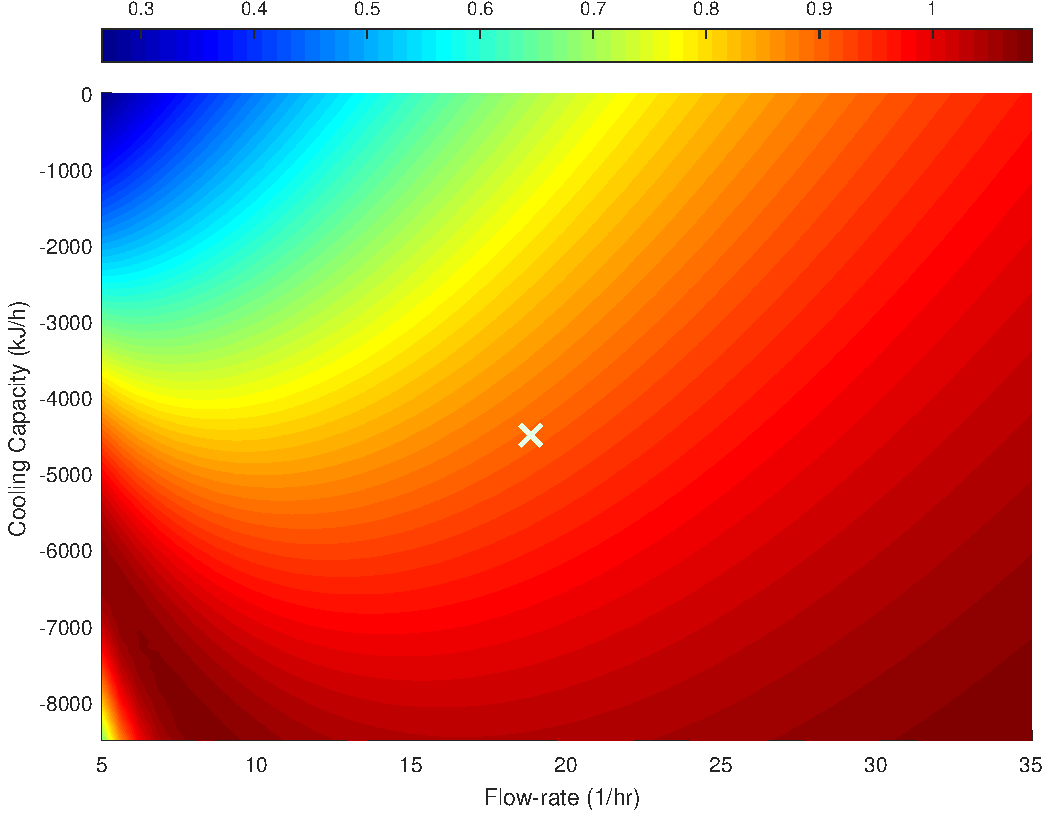
\includegraphics[width=\textwidth]{chapter7/ssValues01}
	\end{subfigure} \hfill
	\begin{subfigure}{0.45\textwidth}
		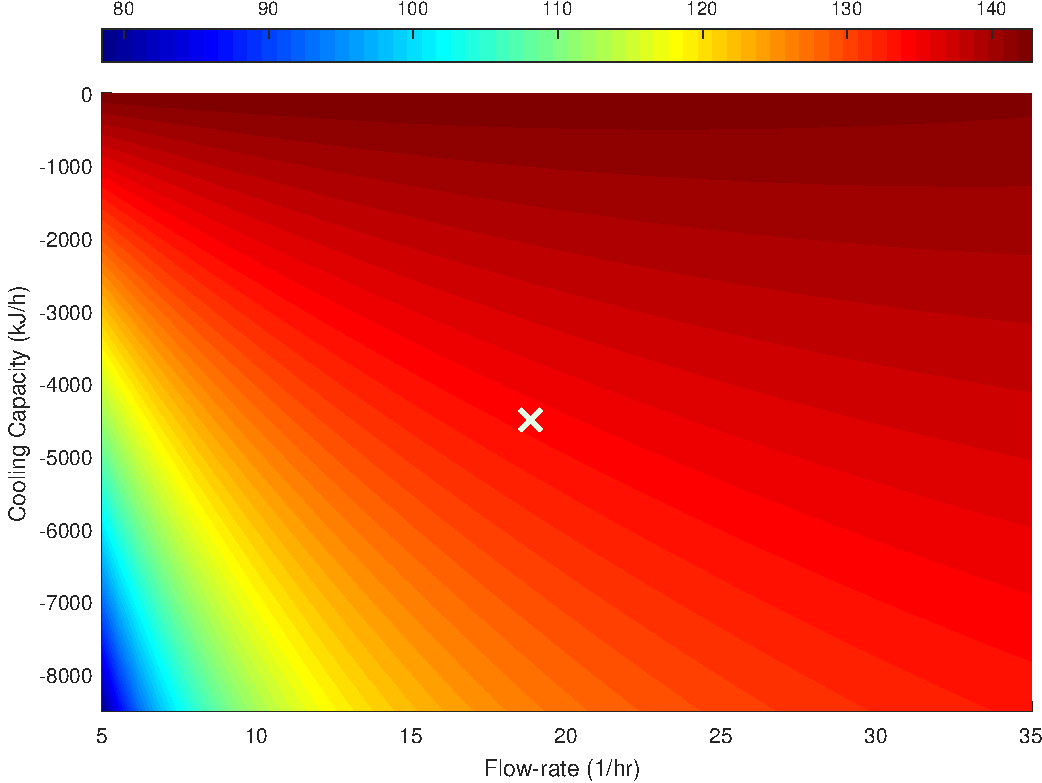
\includegraphics[width=\textwidth]{chapter7/ssValues02}
	\end{subfigure}
	
	\caption{Visualization of the steady-state values for the linearized model.}
	\label{fig:ssValues}
\end{figure}

Using the steady-state values just mentioned, a realization for the linearized model is obtained:
\begin{align}   \label{eq:exoReact01}
\left\{ \begin{matrix*}[l]
    \bm{A} = \begin{bmatrix*}[r]
		  -86.0962 &        0 &  -4.2010 &        0 \\
		   50.6146 & -69.4446 &   0.9958 &        0 \\
		  172.2263 & 197.9985 & -36.7597 &  30.7977 \\
		         0 &       0  &  86.6880 & -86.6880
    \end{bmatrix*} \hfill & &
    \bm{B} = \begin{bmatrix*}[r]
		 3.865  &       0 \\
		-0.900  &       0 \\
		-4.140  &       0 \\
		      0  &  0.100
    \end{bmatrix*} \hfill \\  \\ 
    \bm{C} = \begin{bmatrix}
        0 & 1 & 0 & 0 \\ 0 & 0 & 1 & 0
    \end{bmatrix} \hfill & &
    \bm{D} = \begin{bmatrix}
        0 & 0 \\ 0 & 0 \\ 0 & 0 \\ 0 & 0
    \end{bmatrix} \hfill
\end{matrix*} \right.
.\end{align}

In order to demonstrate that the linear model is a valid approximation of the nonlinear model, both systems were simulated in parallel for the same input signal. The simulation, as shown in Fig. \ref{fig:linear01}, starts at the steady-state values and then apply a sinusoidal change in the input to drag the system away from this initial point. As expected, the results shows that the linearized model is an accurate representation of the system, except when it is far from the steady-state values.

\begin{figure}[ht] \centering
		\begin{tikzpicture}	[node distance=1cm]
		\node (plot) {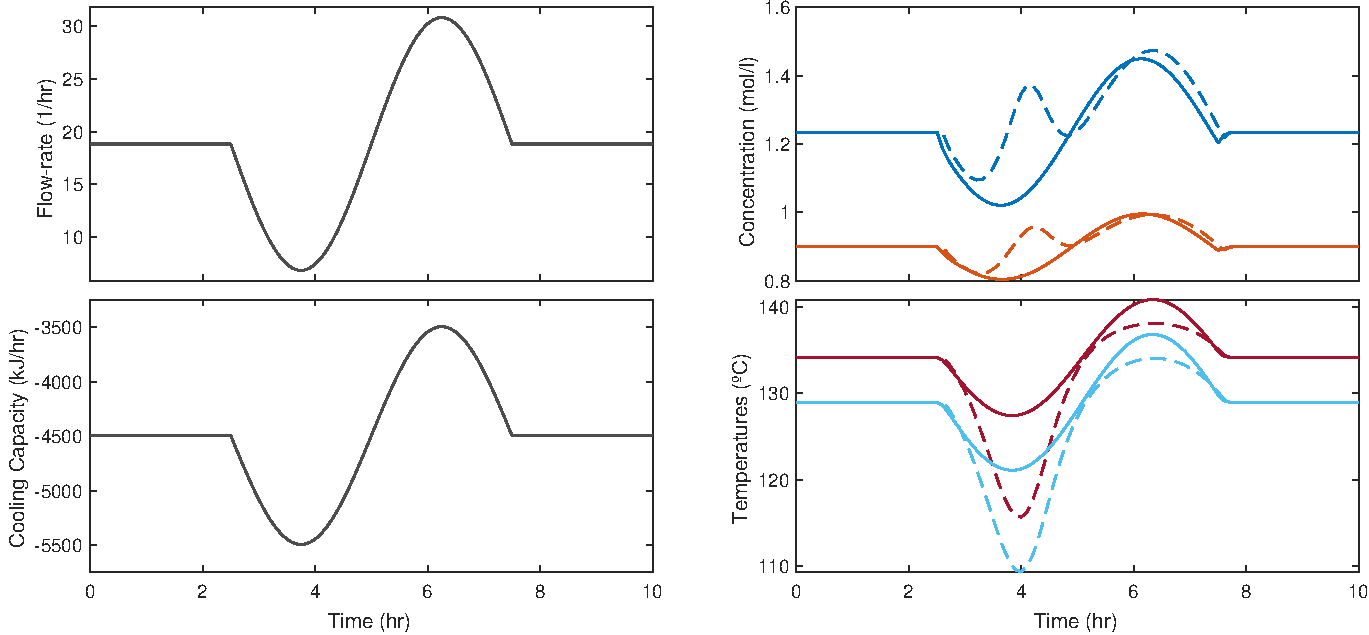
\includegraphics[width=\textwidth]{chapter7/linear01}};
		
		\begin{scope}[on background layer]
			\node[block, above of=plot, xshift=0.65cm, node distance=5.5cm, minimum width=0.7\textwidth] (legendBox) {};
		\end{scope}
		
		\definecolor{linecolor}{rgb}{0, 0.4470, 0.7410};
		\node at (legendBox.west) [xshift=0.6cm]  (legendStart) {};
		\node[right of=legendStart, node distance=1.5cm] (label) {$\rho_A$};		
		\draw[-, linecolor, line width=1.5pt] (legendStart) -- (label);
		
		\definecolor{linecolor}{rgb}{0.8500,0.3250,0.0980};
		\node[right of=label]  (legendStart) {};
		\node[right of=legendStart, node distance=1.5cm] (label) {$\rho_B$};		
		\draw[-, linecolor, line width=1.5pt] (legendStart) -- (label);
		
		\definecolor{linecolor}{rgb}{0.6350, 0.0780, 0.1840};
		\node[right of=label]  (legendStart) {};
		\node[right of=legendStart, node distance=1.5cm] (label) {$T$};		
		\draw[-, linecolor, line width=1.5pt] (legendStart) -- (label);
		
		\definecolor{linecolor}{rgb}{0.3010, 0.7450, 0.9330};
		\node[right of=label]  (legendStart) {};
		\node[right of=legendStart, node distance=1.5cm] (label) {$T_c$};		
		\draw[-, linecolor, line width=1.5pt] (legendStart) -- (label);
	\end{tikzpicture}	
	
	\caption{Simulation of both the nonlinear and linearized State-Space models. The nonlinear response is represented by the dashed lines.}
	\label{fig:linear01}
\end{figure}

%a
%
%\begin{figure}[ht] \centering
%	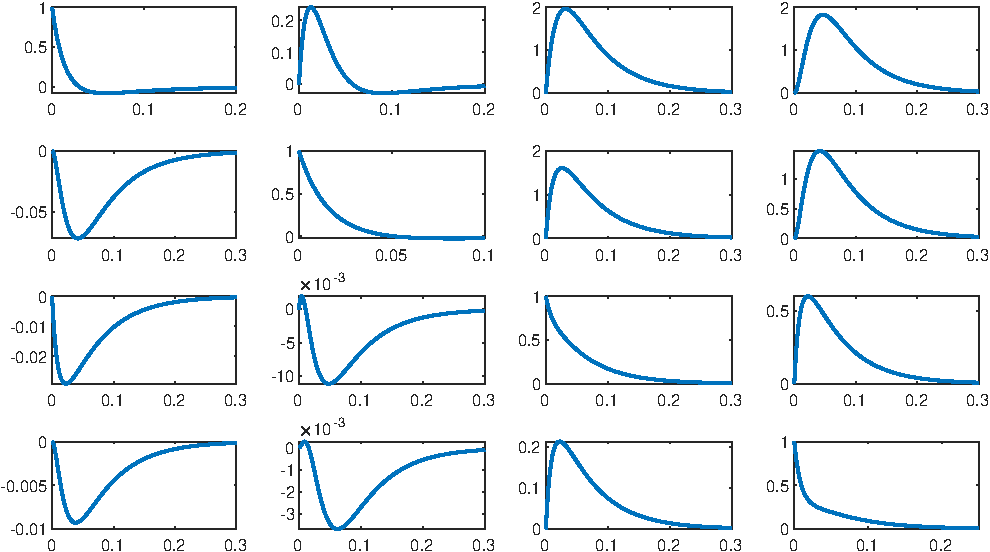
\includegraphics[width=\textwidth]{chapter7/matrixExp01}
%	\caption{a}
%	\label{fig:matrixExp01}
%\end{figure}	


\subsection{Linearized model properties}

Considering a State-Space realization, it is possible to access the system properties. First of all, the BIBO stability of the system was determined through the poles location in the complex plane. In the case of \eqref{eq:exoReact01}, the eigenvalues of $\bm{A}$ were calculated as $\bm{\lambda} = [-16.79, -54.84, -86.33, -121.01]$, which are all in right-hand side of the plane, i.e., $\text{Re}[\lambda_i]$, $\forall i \in [1,4]$. It is possible to conclude that, in the light of this model, the system is stable and does not require a special design for stabilizing controllers.

The next property to be accessed consists in the controllability of the system. Using the definition, the controllability matrix of this model was calculated as:
\begin{equation}
	\bm{\mathcal{C}} = \begin{bmatrix*}[r]
	 3.8650  &      0 & -315.3696  &       0   &  24465 & -12.9 & 2271  \\
   -0.9000   &      0 &  254.0027  &       0   & -32964 & 3.1  & -1250 \\
   -4.1400  &      0  &  639.6409  &  3.0798   & -38589 & -380.2  & 43720 \\
         0  &  0.1000 & -358.8883  &   -8.6688 &  86561 & 1018.5  & -121250 
	\end{bmatrix*}
.\end{equation}

\noindent This matrix has a row rank equal to 4, which is exactly the number of state variables. Therefore, it is concluded that this system is indeed controllable, meaning that it is possible to drive the system to any position in the space using a specific input signal. It is worth mentioning that this matrix exhibits some entries with high values, which can become numerically unstable in the case of augmenting the system.

Moreover, the last property of the system to be accessed concerns the observability of the system. Similarly to the controllability case, the observability matrix was calculated as:
\begin{equation}
	\bm{\mathcal{O}} = \begin{bmatrix*}[r]
         0 &   1.0000 &        0  &       0 \\	
         0 &        0 &   1.0000  &       0 \\ 
   50.6146 & -69.4446 &   0.9958  &       0 \\
  172.2263 & 197.9985 & -36.7597  & 30.7977 \\
   -7701.1 &   5019.7 &  -318.4  &  30.7 \\
   -11137 &  -21028 &   3495 &  -3802 \\
   862270  & -411630  &  51710  & -1246 \\
   496400  &  2152200 &  -432200  &  437200
	\end{bmatrix*}
.\end{equation}

\noindent This matrix has a column rank equal to 4, which, again, is exactly the number of state variables. Thus, it is possible to conclude that the system is observable, meaning that the information of any state can be reconstructed given only the outputs. 

\section{Optimal Control}

\subsection{Regulation}

The results for the controllers arrangements are now presented. The first controller simulated was the Linear Quadratic Regulator (LQR), as shown in Fig. \ref{fig:lqr01}. The simulation started with an initial state $x_1(0) = x_2(0) = 0$ (or, equivalently, $\Delta x_1(0) = -x_{1o}$ and $\Delta x_2(0) = -x_{2o}$) while maintaining the states $x_3$ and $x_4$ at the steady-state value. The goal of this simulation was to represent the scenario where the solution in the tank does not actually contain any concentration of the reagents or products. This scenario, thus, requires that the controller ``starts" the process by providing the flow of reagent necessary to achieve the desirable steady-state concentration of the controlled product. Notice that the resulting reactions will change the temperature inside the tank, requiring also that the controller manipulates the cooling capacity in order to control the reactor temperature.


\begin{figure}[ht] \centering
	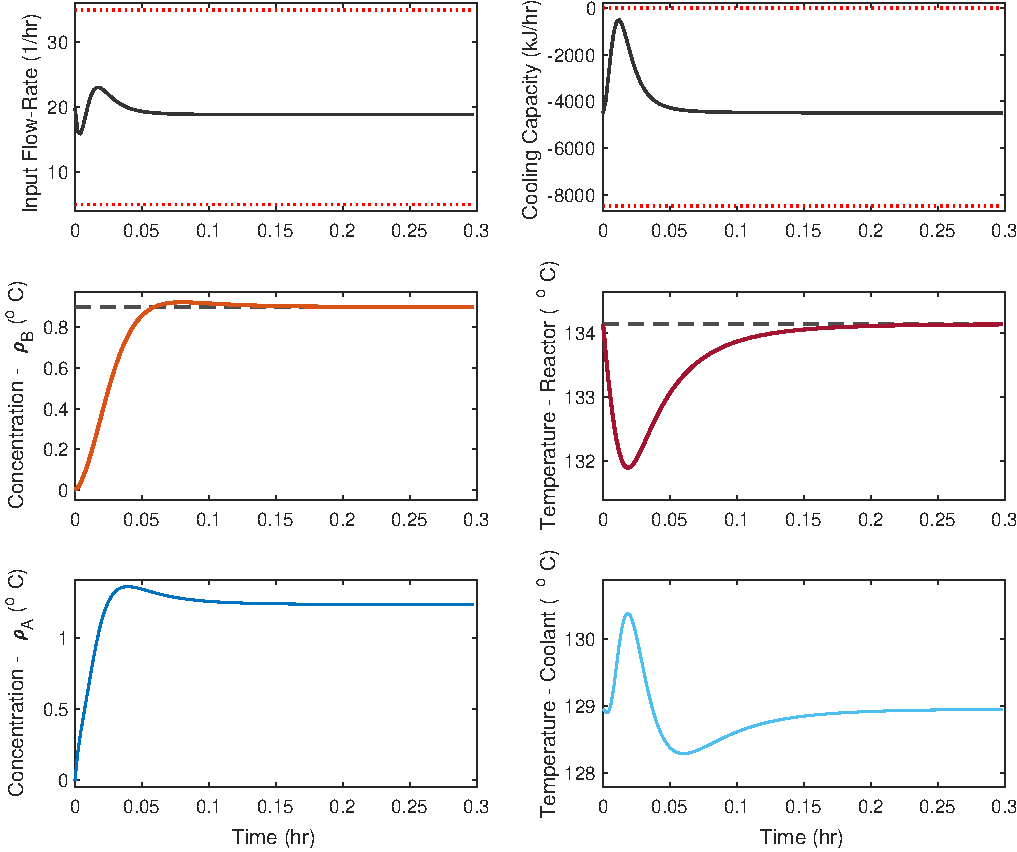
\includegraphics[width=\textwidth]{chapter7/lqr01}
	
	\caption{a}
	\label{fig:lqr01}
\end{figure}

As expected, the controller momentarily increases the input flow-rate in order to accelerate the production of compound $B$, returning to the steady-state value to achieve the desired reference. Notice that the input flow-rate does not grow further in the first minutes in order to avoid overshoots, which occurs in the results presented but with small magnitude. In respect to the reactor temperature, the controller was able to respond to the sudden change by decreasing the absolute value of the cooling capacity, causing the coolant to increase its temperature and, consequently, returns the reactor temperature to the reference. Therefore, the simulation shows that the proposed optimal controller is able to drive the process to a desired constant reference in an optimal manner, not causing overshoots and/or oscillations, in a small amount of time.

\begin{figure}[ht] \centering
	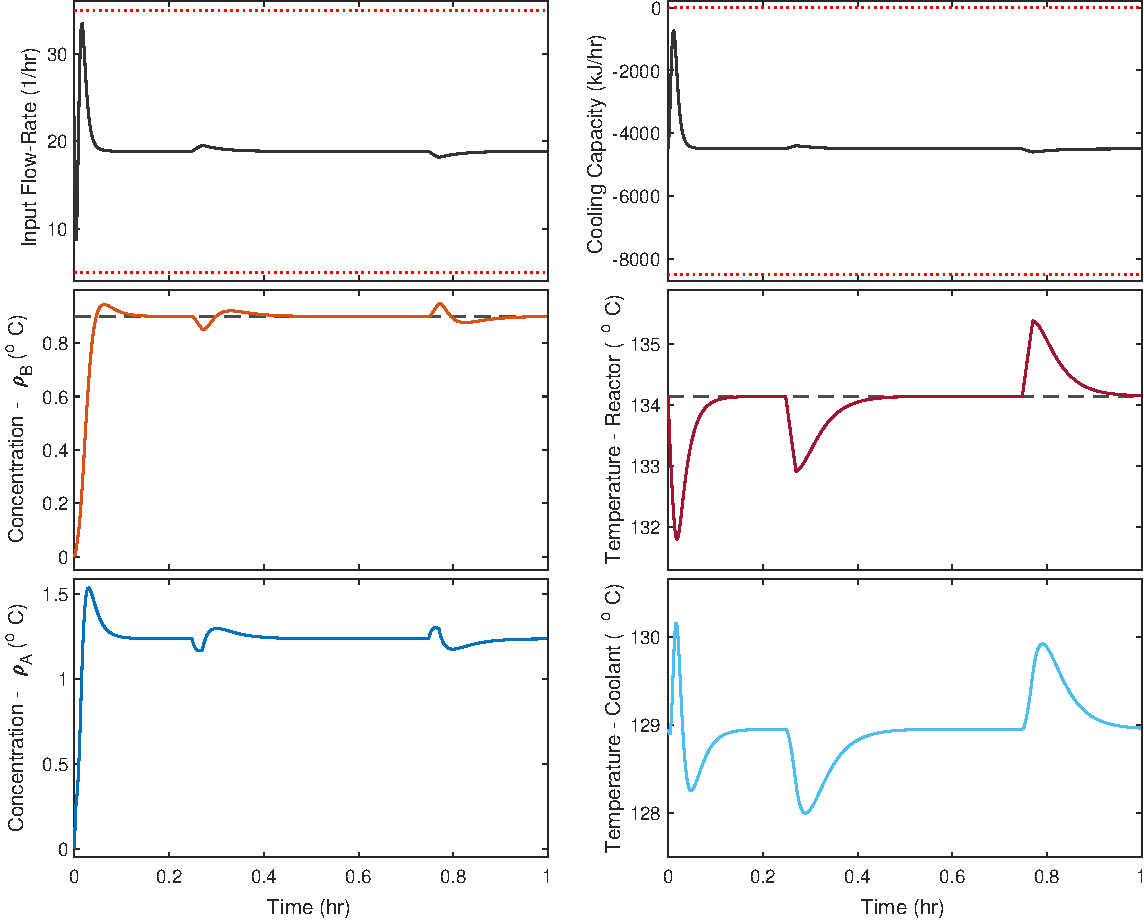
\includegraphics[width=\textwidth]{chapter7/lqr02}
	
	\caption{a}
	\label{fig:lqr02}
\end{figure}	

To further test the capabilities of this controller, the same control objective was considered, but while subjecting the actual system to disturbances in the system variables. Specifically, disturbances were applied to the inflow concentration and temperature, $\rho^{(A)}_{in}$ and $T_{in}$, respectively, to represent the scenario where the fluid entering the tank could be perturbed by previous processes or by instrumentation limitations. To simulate these cases, pulse signals of values $w_1 = \pm 0.5$ and $w_2 = \pm 2$ were applied to the nominal value of the inflow concentration and temperature, respectively. Each pulse starts at an odd multiple of $\lfloor T/4 \rfloor$ and lasts for $0.02T$ hours, where $T$ is the length of the simulation time vector, i.e., the total size of the control horizon. The simulation results are shown in Fig. \ref{fig:lqr02}.

First of all, it was observed that the control horizon had to be increased in order to allow the feedback controller to perceive the disturbance and corrects the system response accordingly. As a direct result of the larger horizon, the controller performed more aggressively at the first minutes. Despite of this, the input signals did not violated the defined constraints for the manipulated variables, indicated at the visualization by the red dotted lines. It was observed that the regulator is capable of react to the disturbances and provide a corrective action to return to the steady-state point. 

Until now, the experiments were done assuming that the optimal controller had direct access to the real system states. In a more realistic scenario, the states can only be reconstructed through noisy measurements of the system output. A Linear Quadratic Gaussian (LQG) controller is proposed to deal with this limitation, considering the same control objectives of the previous experiments. In the next simulations it was assumed a process noise $\bm{w} : \mathbb{R} \rightarrow \mathbb{R}^{4}$ and measurement noise $\bm{z} : \mathbb{R} \rightarrow \mathbb{R}^{2}$ described by the following Gaussian distributions:
\begin{equation}
\begin{matrix}
	\bm{w}(t) \sim \mathcal{N}\left( \begin{bmatrix} 0 \\ 0 \\ 0 \\ 0 \end{bmatrix}, \begin{bmatrix} 0.1 & 0 & 0 & 0 \\ 0 & 0.1 & 0 & 0 \\ 0 & 0 & 0.1 & 0 \\ 0 & 0 & 0 & 0.1 \end{bmatrix} \right) & 
\bm{z}(t) \sim \mathcal{N}\left( \begin{bmatrix} 0 \\ 0 \end{bmatrix}, \begin{bmatrix} 0.0001 & 0 \\ 0 & 0.1 \end{bmatrix} \right)
\end{matrix}
\end{equation}

The covariance matrix of the noise $\bm{w}(t)$ tries represents the uncertainty of the non-linear model behavior in respect to the linearized model, while the covariance matrix of $\bm{z}(t)$ aims to represent realistic limitation of measurement devices in respect to these variables. Initially, it is assumed that the Kalman-Bucy estimator can accurately estimate these covariances before optimizing each estimator gain $\bm{K}_e(t)$. The simulation results, for the scenario of starting the process, is shown in Fig. \ref{fig:lqg01}.
 
\begin{figure}[ht] \centering
	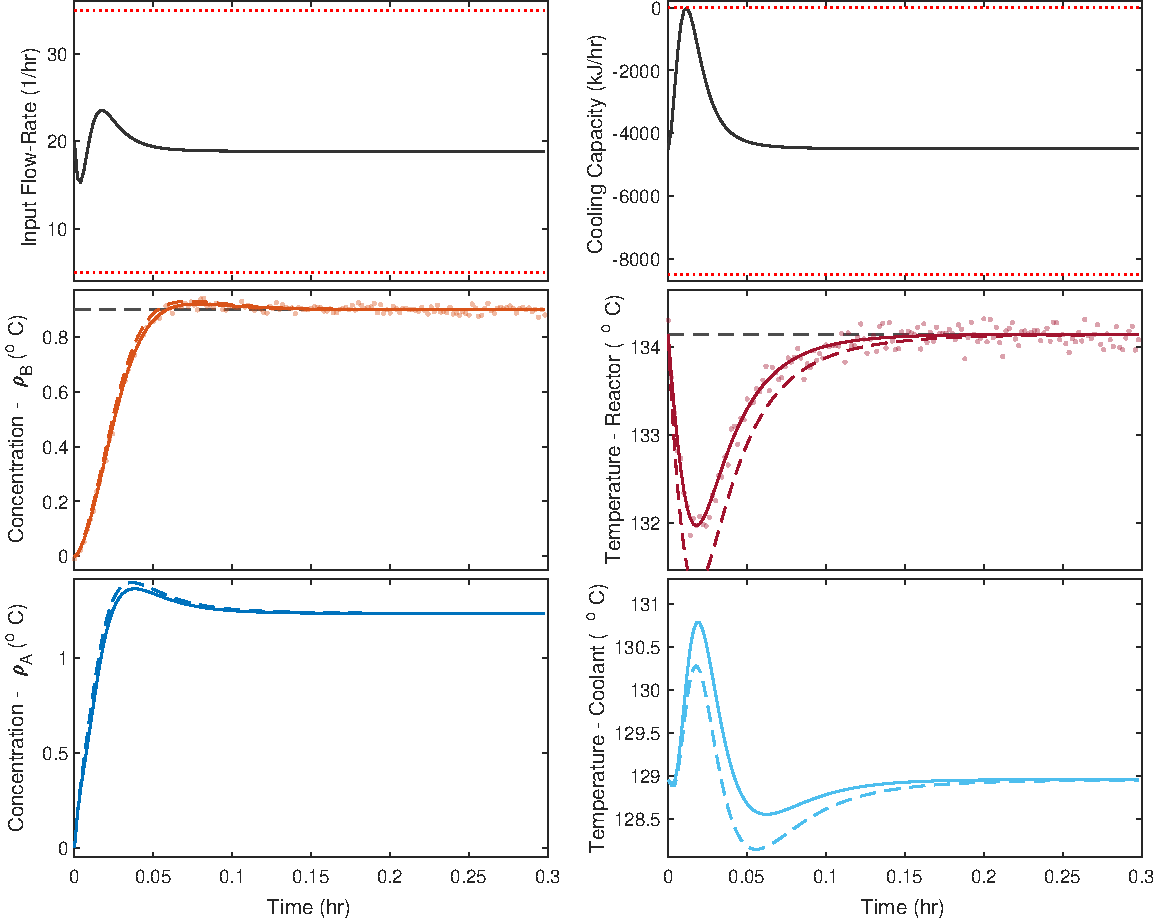
\includegraphics[width=\textwidth]{chapter7/lqg01}
	\caption{a}
	\label{fig:lqg01}
\end{figure}

The estimation of the covariance matrices gave the estimator enough information to accurately reconstruct the state vector from the observations. As it can be seen in the visualizations, this control-estimation operation is very similar to the one shown in Fig. \ref{fig:lqr01}, when the states were directly known. It is visible, however, a slightly greater peak value for the cooling capacity in this case. Thus, the LQG controller proved to be optimal even for in realistic configurations.

Furthermore, the same controller was also evaluated for the case where disturbances in the system variables are present. In this experiment, the same disturbance signal used in the LQR simulation is provided to the observed system. The results are shown in Fig. \ref{fig:lqg02}.

\begin{figure}[ht] \centering
	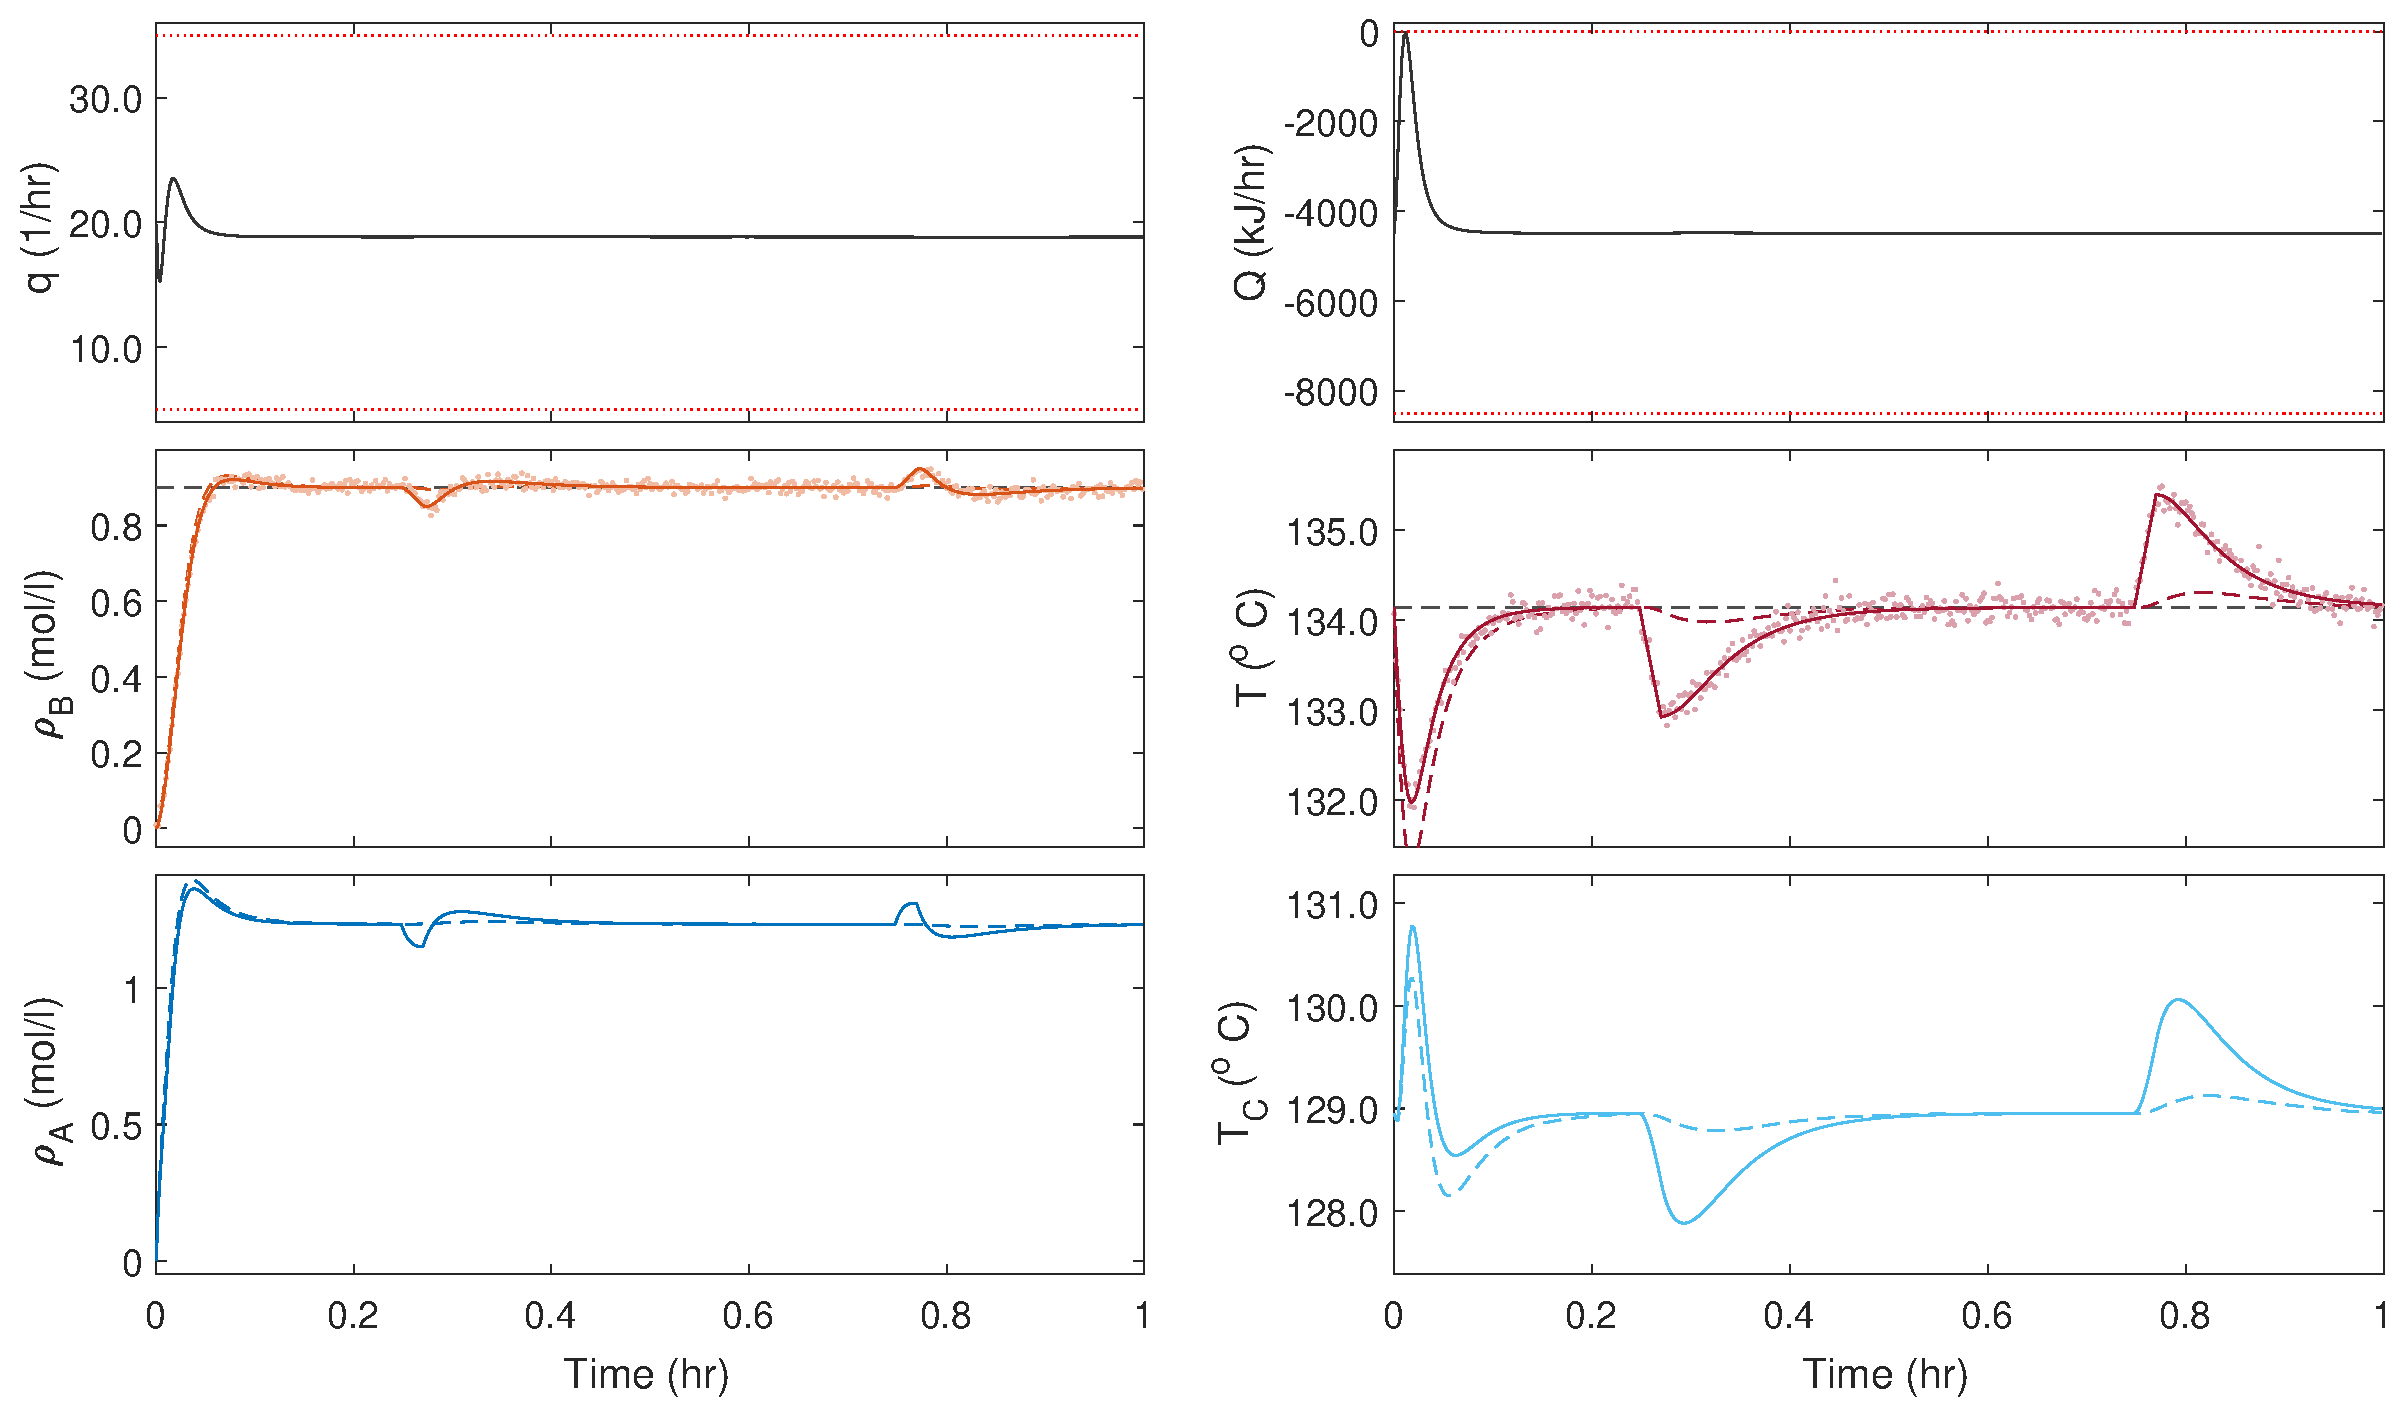
\includegraphics[width=\textwidth]{chapter7/lqg02}
	\caption{a}
	\label{fig:lqg02}
\end{figure}	

Doing a comparison with Fig. \ref{fig:lqr01}, it seems that the system responses are very similar. However, the controller in this case performed less aggressively, which resulted in a more damped response for the concentrations, in the beginning of the operation. The corrective actions for the disturbances were also smoother than of those before, and they are barely visible in the scale of the visualization. Finally, the performance metrics for the discussed controllers are displayed in Table \ref{tb:lqrMetrics}.

\begin{table}[ht]
	\centering
	\begin{tabular}{l | c c | c c c c}
		\textbf{Controller} & $\bm{Q}_{\Delta}$ & $\bm{R}_{\Delta}$ & \textbf{ISE} & \textbf{IAE} & \textbf{ITSE} & \textbf{ITAE} \\
		\hline
		$LQR_1$ & $\begin{bmatrix} 1 & 1 & 1 & 1 \end{bmatrix}$ & $\begin{bmatrix} 1 & 1 \end{bmatrix}$ & $\begin{pmatrix} 1 \\ 1 \end{pmatrix}$ & $\begin{pmatrix} 1 \\ 1 \end{pmatrix}$	& $\begin{pmatrix} 1 \\ 1 \end{pmatrix}$ & $\begin{pmatrix} 1 \\ 1 \end{pmatrix}$ \\
		$LQR_2$ & $\begin{bmatrix} 1 & 1 & 1 & 1 \end{bmatrix}$ & $\begin{bmatrix} 1 & 1 \end{bmatrix}$ & $\begin{pmatrix} 1 \\ 1 \end{pmatrix}$ & $\begin{pmatrix} 1 \\ 1 \end{pmatrix}$	& $\begin{pmatrix} 1 \\ 1 \end{pmatrix}$ & $\begin{pmatrix} 1 \\ 1 \end{pmatrix}$ \\
		$LQR_3$ & $\begin{bmatrix} 1 & 1 & 1 & 1 \end{bmatrix}$ & $\begin{bmatrix} 1 & 1 \end{bmatrix}$ & $\begin{pmatrix} 1 \\ 1 \end{pmatrix}$ & $\begin{pmatrix} 1 \\ 1 \end{pmatrix}$	& $\begin{pmatrix} 1 \\ 1 \end{pmatrix}$ & $\begin{pmatrix} 1 \\ 1 \end{pmatrix}$ \\
		$LQR_4$ & $\begin{bmatrix} 1 & 1 & 1 & 1 \end{bmatrix}$ & $\begin{bmatrix} 1 & 1 \end{bmatrix}$ & $\begin{pmatrix} 1 \\ 1 \end{pmatrix}$ & $\begin{pmatrix} 1 \\ 1 \end{pmatrix}$	& $\begin{pmatrix} 1 \\ 1 \end{pmatrix}$ & $\begin{pmatrix} 1 \\ 1 \end{pmatrix}$ \\
	\end{tabular}
	
	\caption{•}
	\label{tb:lqrMetrics}
\end{table}

\subsection{Tracking}

Now, the experiments for controllers that track non-constant references is presented. As in the previous subsection, the first controller simulated consists in the Linear Quadratic Regulator with Integral Action (LQRI), also known as Linear Quadratic Servo (LQ-Servo). The simulations starts with initial states equal to the steady-state values. The proposed scenario for this controller is to increase and then decrease the amount of compound $B$ that is produced, while maintaining the reactor temperature at a constant value. For the concentration control, the reference signal is comprised by a sequence of step functions which varies from approximately $12\%$ of the operation value, which is a realistic set-point change in such processes. The results of the simulation are shown in Fig. \ref{fig:lqri01}.

\begin{figure}[ht] \centering
	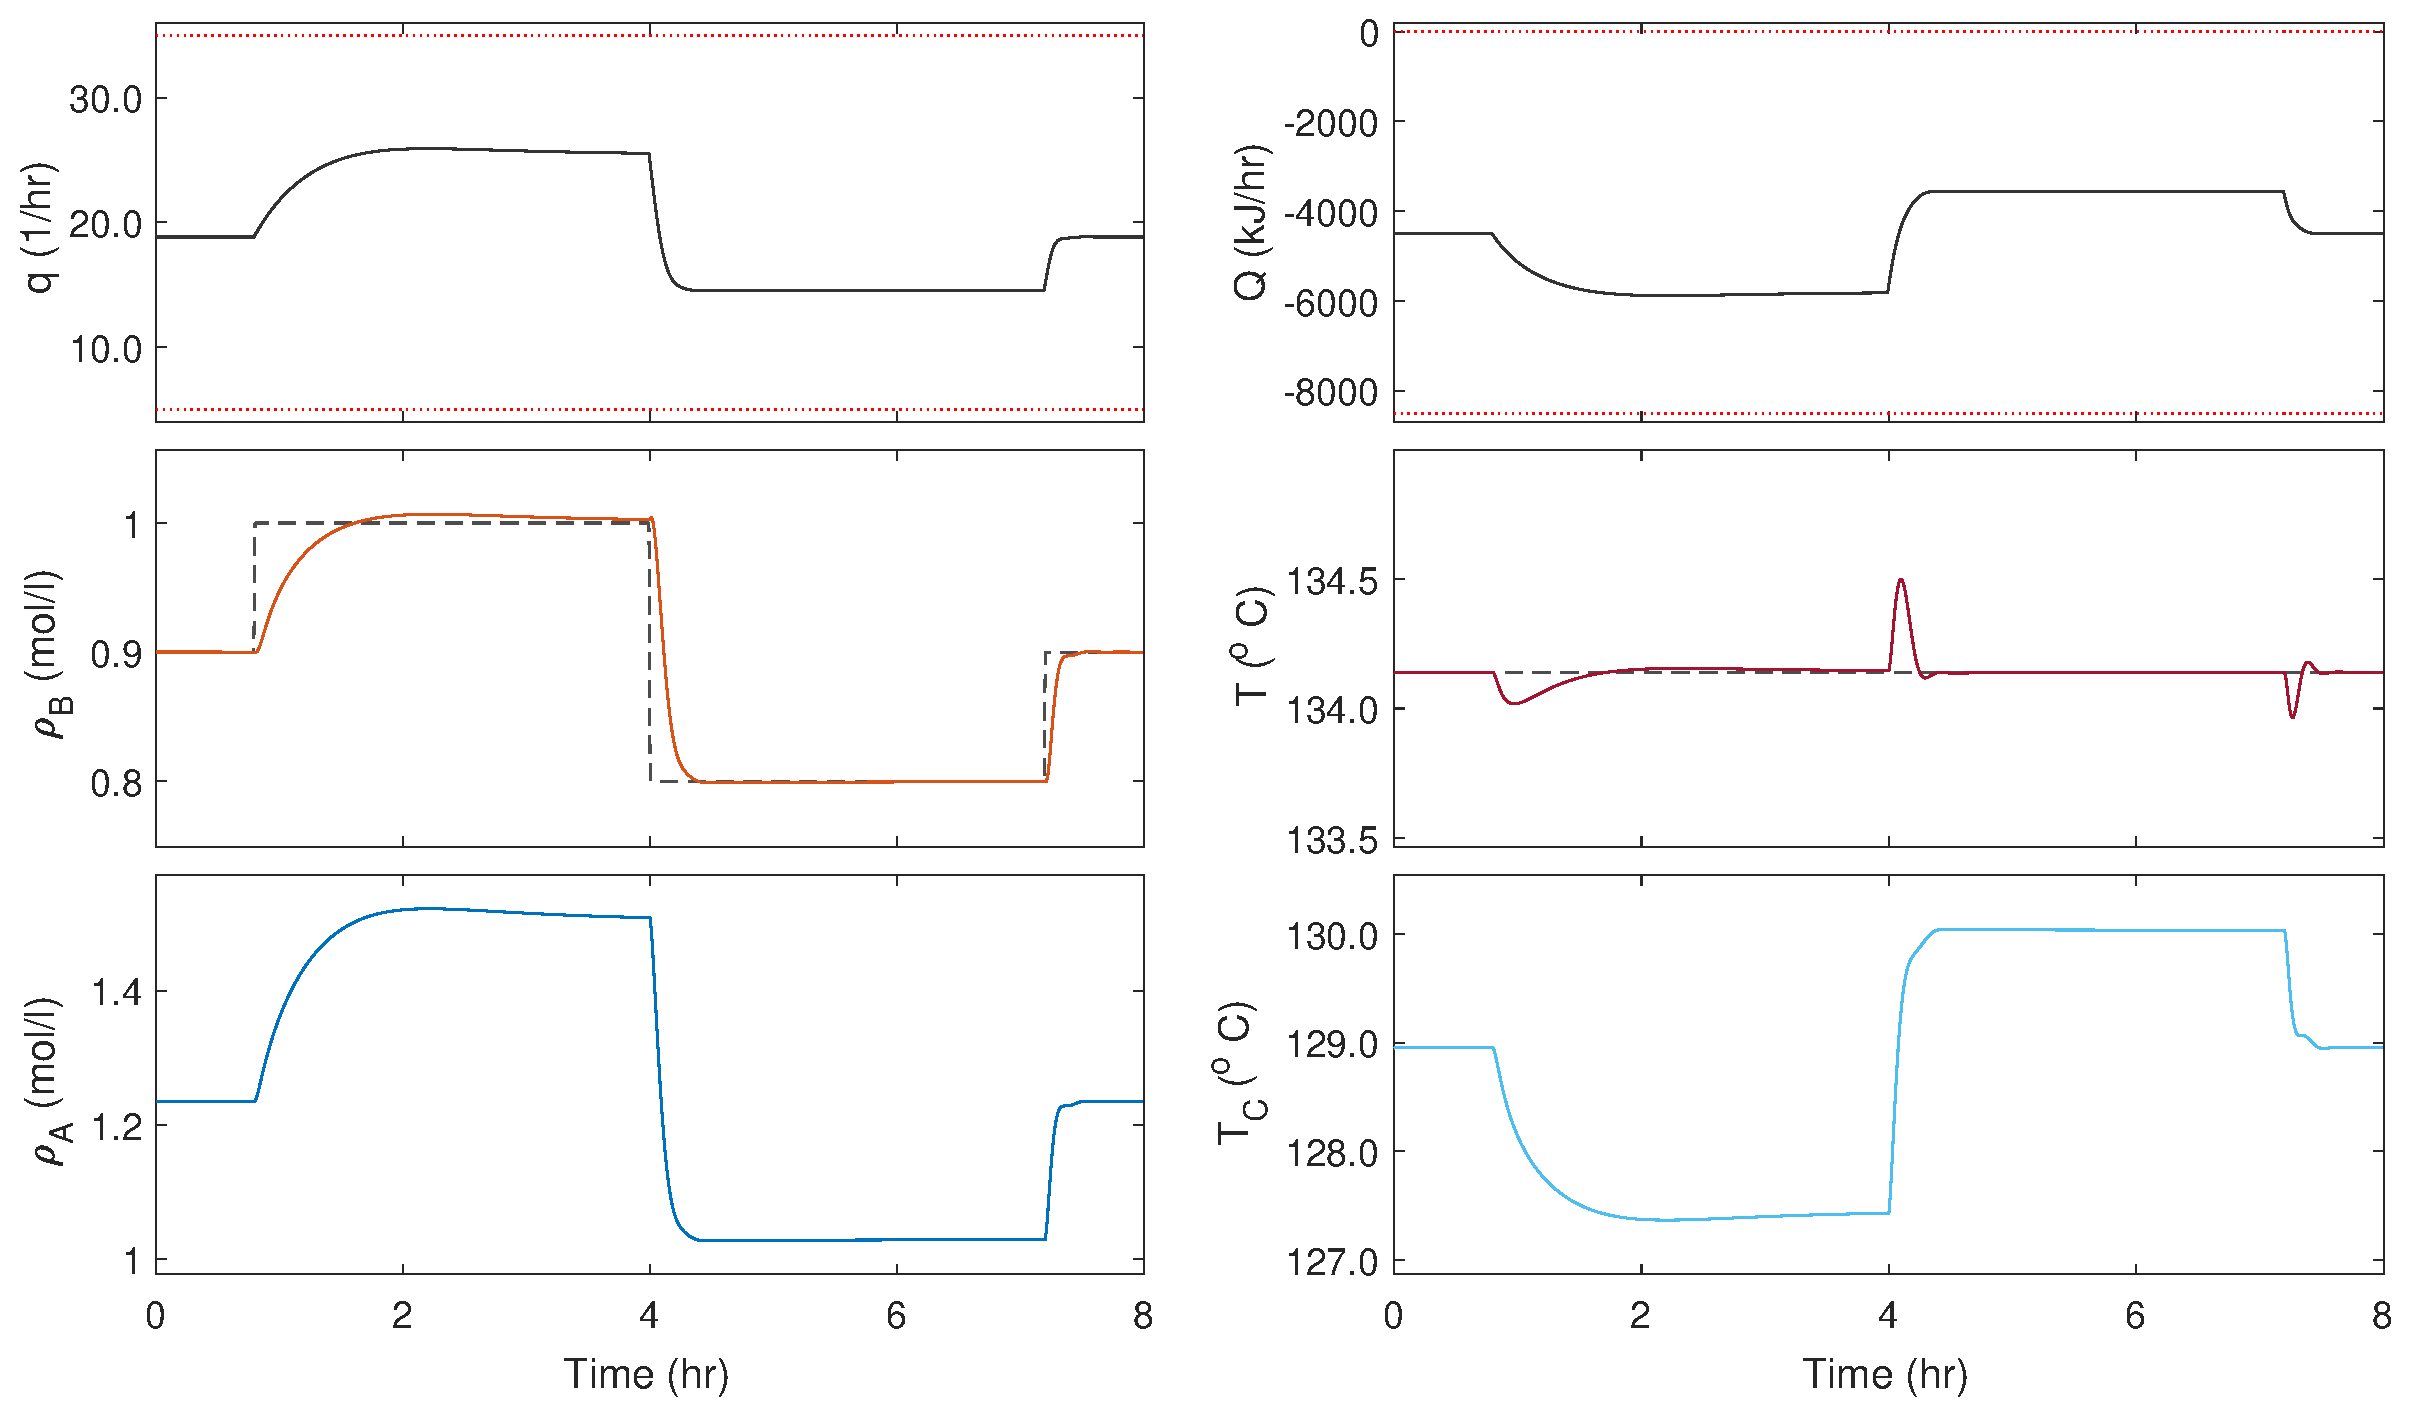
\includegraphics[width=\textwidth]{chapter7/lqri01}
	
	\caption{a}
	\label{fig:lqri01}
\end{figure}

After the introduction of the integral action, two more weights were needed to be selected for the controller optimization. As expected, the MIMO case actually imposes a trade-off between reaching the reference for the concentration and for the temperature, in the case that they do not represent a valid steady-state. Therefore, the choices of weights to the integral action has to take in account the fact that an aggressive set-point tracking may result in oscillatory, or even unstable, systems. To avoid these situations, the weights were selected to cause a smooth tracking, and the control horizon was expanded to allow the controller to operate for more hours. 

Despite the mentioned difficulties, the controller was able to drive the system as close as possible to the reference, while still obeying the manipulated variables constraints. Notice that, in the moments were the reference changes, the change in the concentration resulted in a momentarily change in the temperature, which is promptly corrected by the feedback action of the controller. This change, however, is very small and the temperature remained within an interval of $0.5ºC$ around the reference signal, which is an excellent result. Another nice response observed in the visualization comprises in the change in the coolant temperature, which follows closely the shape of the change in the cooling capacity. In the last simulations, this variable evolved in a similar manner to the reactor temperature, but, in this case, the first was directly manipulated to allow for the latter to stay at the steady-state value.

Following the same case of the previous subsection, the same controller was used to simulate a closed-loop operation in the case when disturbances to the real system are occurring. In this case, a pulse signal is applied to the same variables as in the last case, but for each time instant multiple of $\lfloor T/4 \rfloor$ with a duration of $0.02T$, which is a longer step in this case since $T$ is greater. The results are presented at Fig. \ref{fig:lqri02}. 

\begin{figure}[ht] \centering
	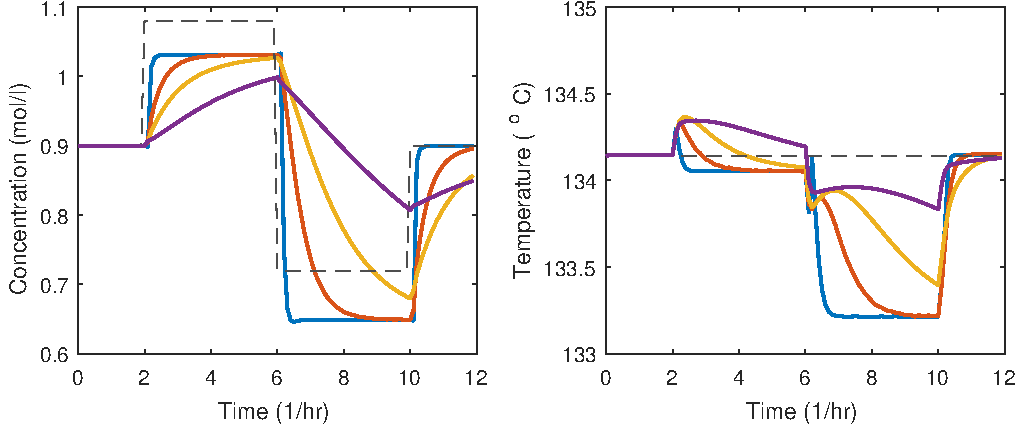
\includegraphics[width=\textwidth]{chapter7/lqri02}
	
	\caption{a}
	\label{fig:lqri02}
\end{figure}	

The first interesting phenomena to notice is that the system responded more aggressively to the disturbances that occurred between the time interval $t \in [0.8, 4]$ for which $r(t) = 1$, when compared to the disturbances occurring in the interval $t \in [4, 7.2]$ for which $r(t) = 0.8$. This is expected from the fact that the system has non-linear terms associated with the concentration $\rho_A$, which is greater at the first interval. The controller, however, was able to correct the disturbances and drive the system back to the reference in both cases, exhibiting a smoother response in the latter.

In the direction for a more realistic scenario, the same reference tracking just proposed was used together with a Linear Quadratic Gaussian, augmented with integral action, to perform the feedback over the estimated states. In this case, the integral of the error was calculated directly from the noise measurements, rather from an output calculated from the estimated states. The process and measurement noises used were the same as in the regulation case, and the covariance matrices were estimated directly from the noise signals. The resulting operation is displayed at Fig. \ref{fig:lqg01}.

\begin{figure}[ht] \centering
	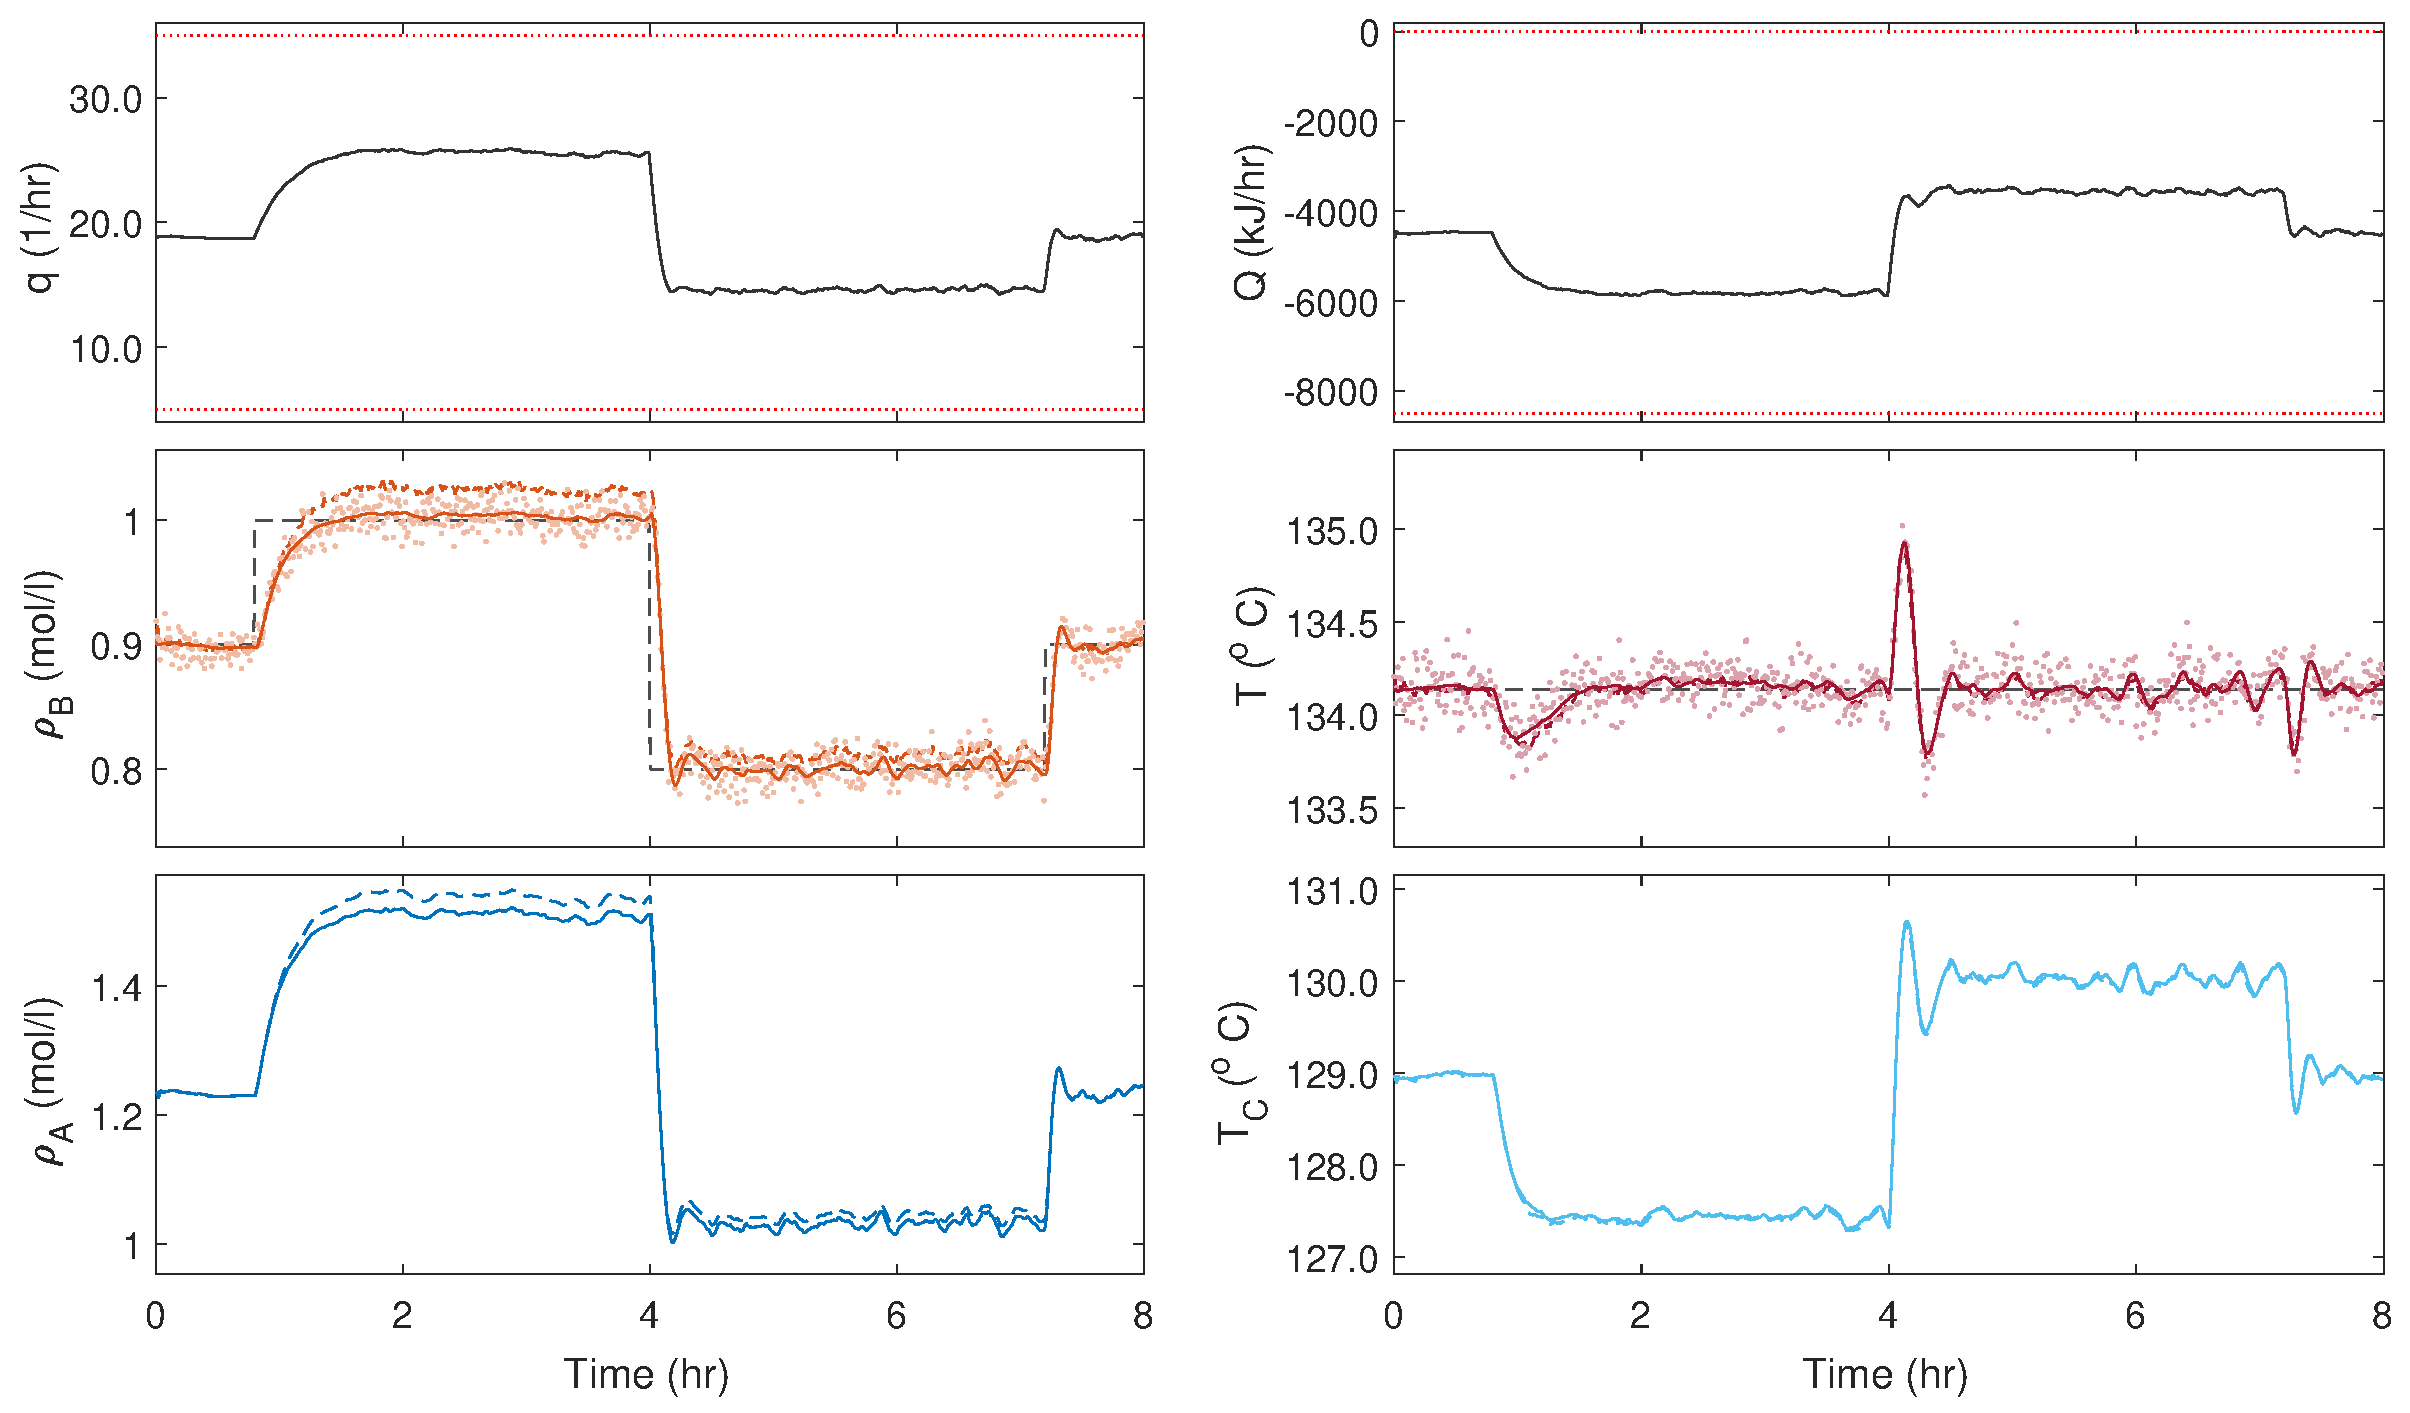
\includegraphics[width=\textwidth]{chapter7/lqgi01}
	\caption{a}
	\label{fig:lqgi01}
\end{figure}

The first difference noted was the fact that the weights for the augmented states for the LQG controller actually needed a value of greater magnitude than those used for the LQR case. Despite of this, the information on the covariances were enough to allow for an accurate estimation of the real system states, and the control performed was very similar to that obtained when directly accessing the system real states, just as expected. However, it is noticeable that the input signals yielded by the controller were actually smoother and resulted in an apparent better tracking. This can be explained by the fact that the assignment of weights for the augmented states allowed for a better trade-off between the concentration and temperature tracking, resulting in a smaller deviance.

For completeness, the same tracking objective was simulated for the case of disturbances actuating on the real system, just as in the previous cases, as shown in Fig. \ref{fig:lqgi02}. The resulting control was actually similar to the case observed from directly accessing the states. This fact proves the feasibility of using controller-estimator configurations for reference tracking control, even in the presence of disturbances to the process. 

\begin{figure}[ht] \centering
	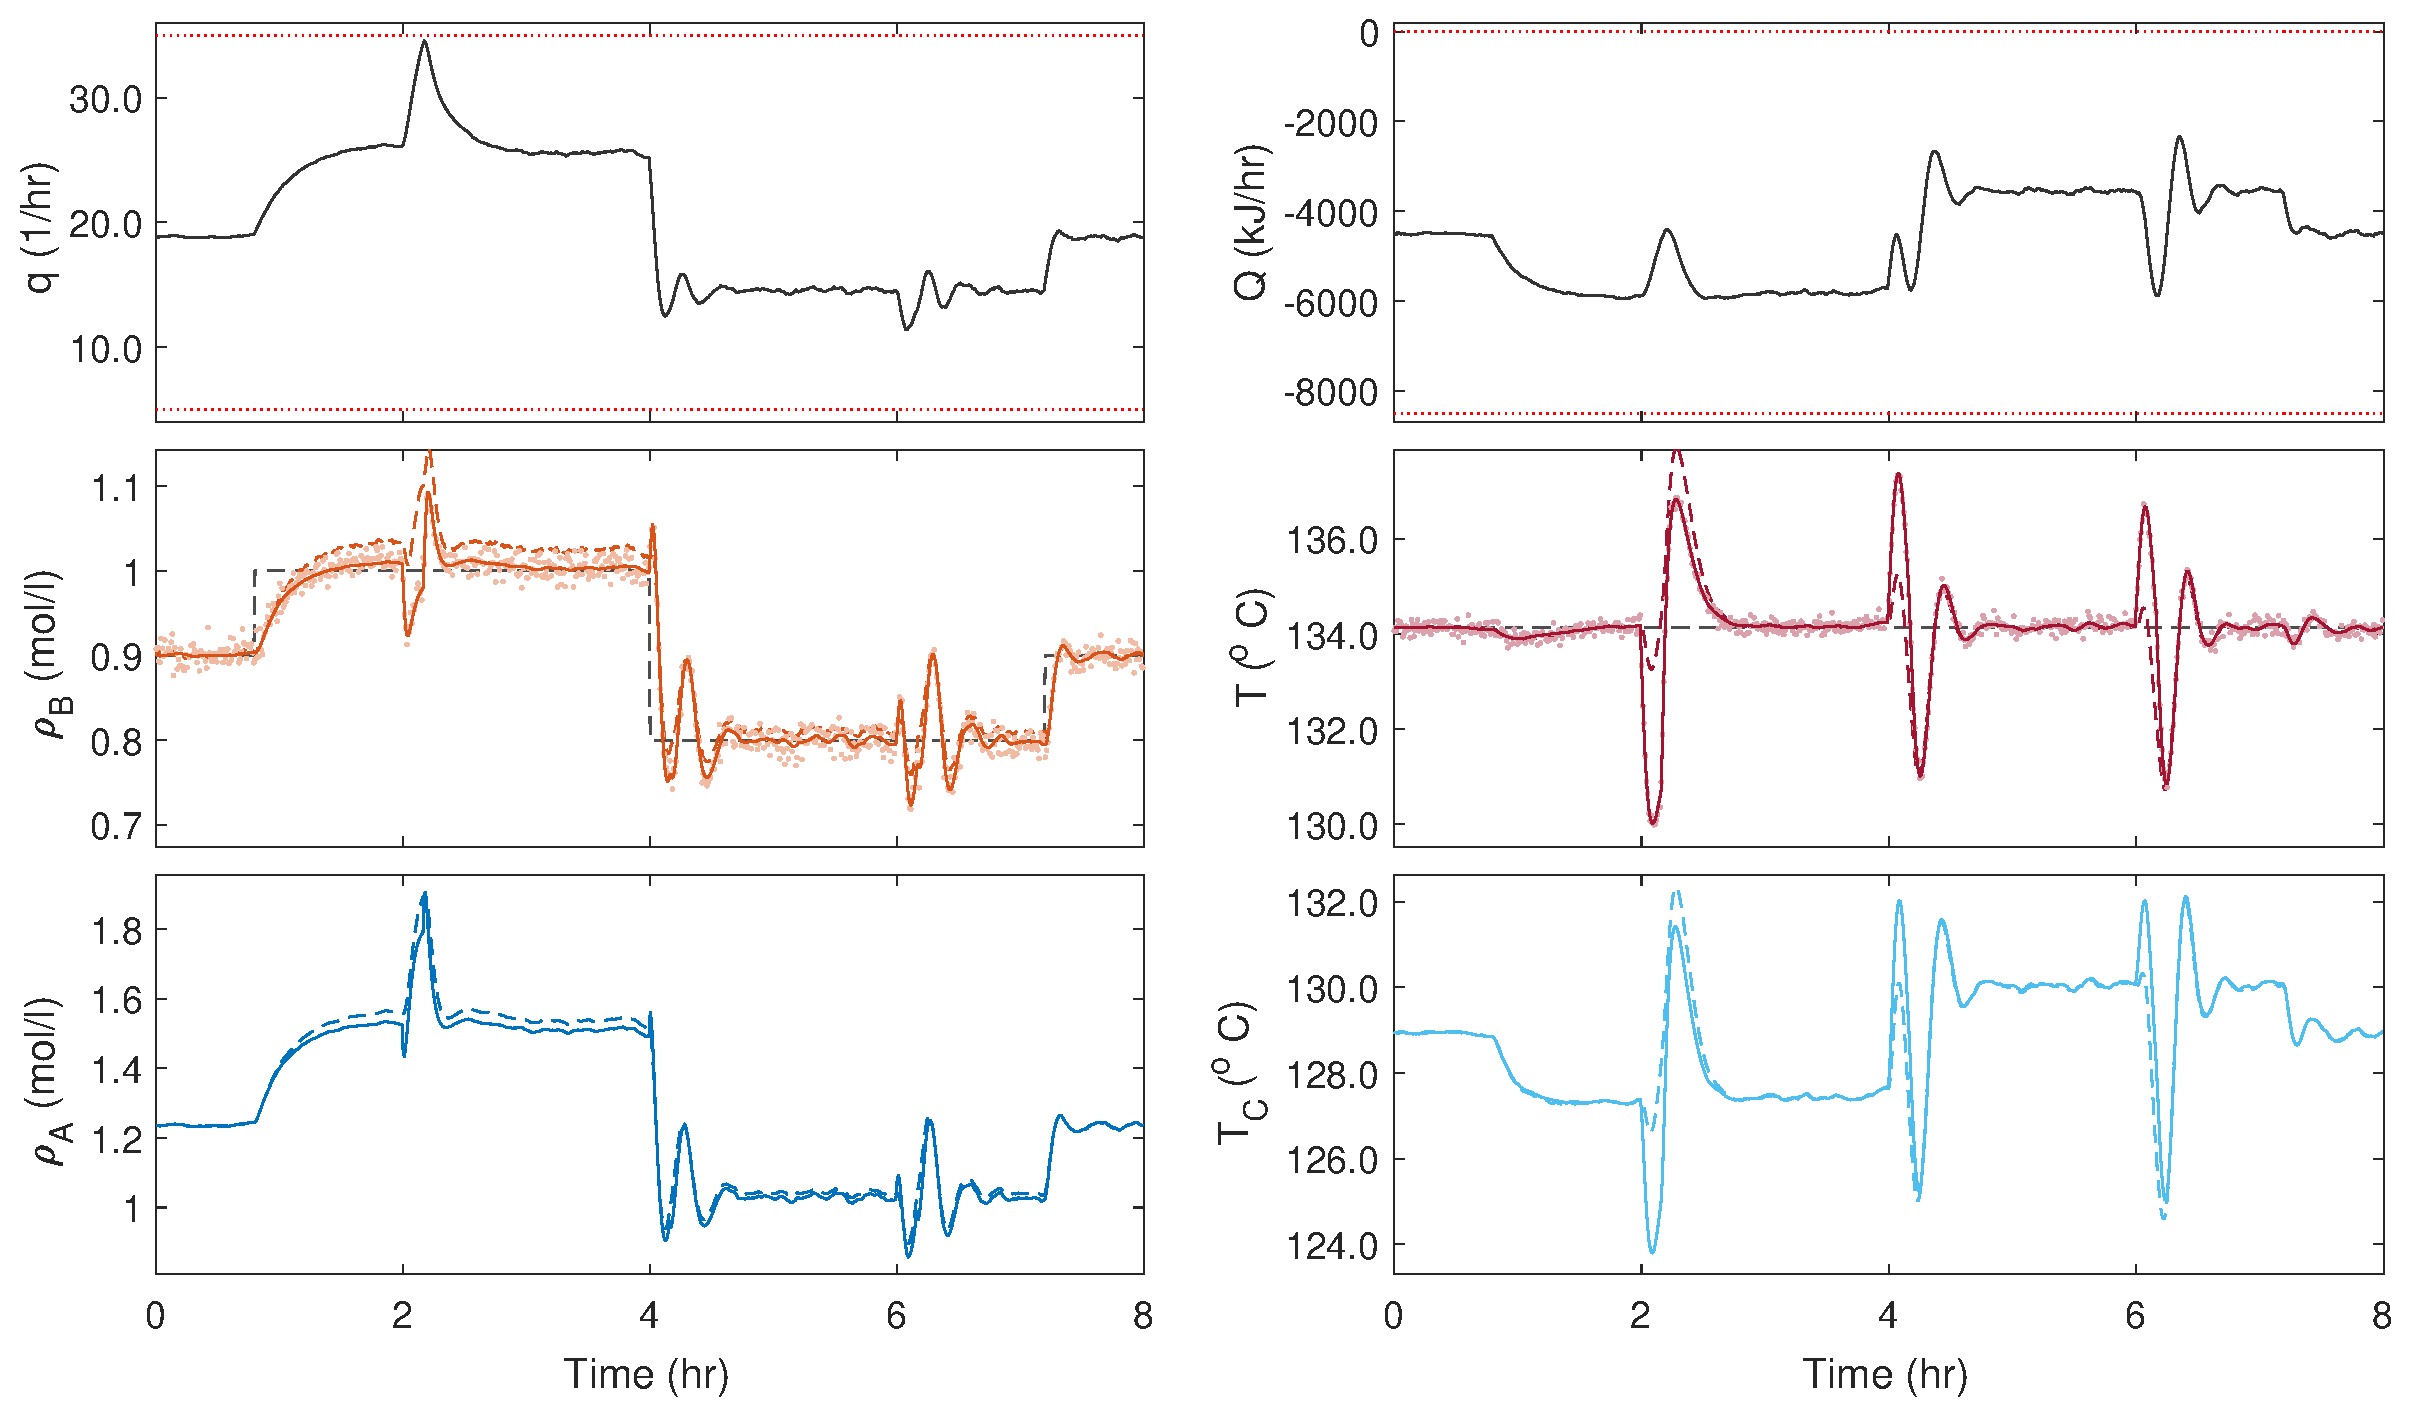
\includegraphics[width=\textwidth]{chapter7/lqgi02}
	\caption{a}
	\label{fig:lqgi02}
\end{figure}	

% 8 - Conclusion
% ---------------------------------------------------------------
\clearpage
\chapter{Conclusion}

This work has presented a self-contained mathematical framework to model and control chemical reactor systems, focusing on optimal control techniques. In this document, several results were presented and discussed in order to provide a complete understanding of the concepts and methods explored. The discussed methods were applied to a given model of a challenging real-world chemical reactor, which consists of a non-isothermal process following the Van de Vusse reaction scheme. The experiments have shown that optimal control is a feasible solution when the controller has direct access to the internal states of the system, but performed worse when the states are not accessible but estimated. The control simulations, however, still produced practical results that are realistic in respect to real plant of such processes.

The use of optimal controllers greatly reduces the complexity of the controller synthesis procedure, while ensuring an optimal operation. The methods presented can still be expanded to more complex formulations, which would allow for better performance in more adverse cases. Specifically, more advanced state estimation techniques can be considered to mitigate the problem of reference tracking, determining the integral action through an estimate of the controlled variables.

This work also emphasizes the possibility of formulating more advances techniques, within the scope of optimal control, to achieve better results. As future work, there is the necessity to decouple the control and estimator sample time from the continuous-time in which the real system operates, providing a more realistic configuration of feedback control loops. Additionally, non-linear state estimation techniques should be explored to solve the linearized Kalman filter limitation, and constrained optimal controllers should be explored to mathematically ensure that the hard constraints of the system are being respected.

% A - Apêndice A
% ---------------------------------------------------------------
\clearpage
\appendix
\chapter{Properties of Gaussian Distributions}

\begin{boxed-definition}{(Gaussian Distribution)} \label{def:gauss}
	A random variable $\bm{x} \in \mathbb{R}^n$ has a Gaussian distribution with mean $\bm{\mu} \in \mathbb{R}^n$ and covariance $\bm{\Sigma} \in \mathbb{R}^{n \times n}$, denoted as $\bm{x} \sim \mathcal{N}(\bm{x}|\bm{\mu}, \bm{\Sigma})$, if its probability density is described as:
	\begin{equation}
		\mathcal{N}(\bm{x}|\bm{\mu}, \bm{\Sigma}) = \cfrac{1}{(2\pi)^{n/2} | \bm{\Sigma} |^{1/2}} exp \left\{-\cfrac{1}{2} (\bm{x} - \bm{\mu})^T \Sigma^{-1} (\bm{x} - \bm{\mu}) \right\}
	.\end{equation}
\end{boxed-definition}

\begin{boxed-lemma}{(Joint distribution of Gaussians)} \label{le:jointGauss}
	Consider the random variables $\bm{x} \in \mathbb{R}^n$ and $\bm{y} \in \mathbb{R}^m$, which have the Gaussian distributions
	\begin{equation}
		\begin{matrix*}[l]
			p(\bm{x})\phantom{|x} = \mathcal{N}(\bm{\mu}, \bm{\Sigma}), \hfill \\
			p(\bm{y}|\bm{x}) = \mathcal{N}(\bm{A} \bm{x} + \bm{u}, \bm{L}),
		\end{matrix*}
	\end{equation}
	
	\noindent then the distribution of $(\bm{x}, \bm{y})$ and the marginal distribution of $\bm{y}$ are given as:
	\begin{equation}
	\begin{split}
		p\left( \begin{bmatrix} \bm{x} \\ \bm{y} \end{bmatrix} \right) &= \mathcal{N}\left( \left. \begin{bmatrix} \bm{x} \\ \bm{y} \end{bmatrix} \right| \begin{bmatrix} \bm{\mu} \\ \bm{A} \bm{\mu} + \bm{u} \end{bmatrix}, \begin{bmatrix} \bm{\Sigma} & \bm{\Sigma} \bm{A}^T \\ \bm{A} \bm{\Sigma} & \bm{A} \bm{\Sigma} \bm{A}^T + \bm{L} \end{bmatrix} \right), \\
		p(\bm{y})  &= \mathcal{N} \left( \bm{A} \bm{\mu} + u, \bm{A} \bm{\Sigma} \bm{A}^T + \bm{L} \right).
	\end{split}			
	\end{equation}
\end{boxed-lemma}

\begin{boxed-lemma}{(Conditional distribution of Gaussians)} \label{le:condGauss}
	Consider the random variables $\bm{x} \in \mathbb{R}^n$ and $\bm{y} \in \mathbb{R}^m$, which have the joint Gaussian distribution
	\begin{equation}
		p\left( \begin{bmatrix} \bm{x} \\ \bm{y} \end{bmatrix} \right) = \mathcal{N}\left( \left. \begin{bmatrix} \bm{x} \\ \bm{y} \end{bmatrix} \right| \begin{bmatrix} \bm{\mu}_{x} \\ \bm{\mu}_{y} \end{bmatrix}, \begin{bmatrix} \bm{\Sigma}_{xx} & \bm{\Sigma}_{xy} \\ \bm{\Sigma}_{xy}^T & \bm{\Sigma}_{yy} \end{bmatrix} \right),
	\end{equation}
	
	\noindent then the marginal and conditional distributions of $\bm{x}$ and $\bm{y}$ are given as:
	\begin{equation}
	\begin{split}
		p(\bm{x}) &= \mathcal{N}(\bm{x} | \bm{\mu}_{x}, \bm{\Sigma}_{xx}), \\
		p(\bm{y}) &= \mathcal{N}(\bm{y} | \bm{\mu}_{y}, \bm{\Sigma}_{yy}), \\
		p(\bm{x}|\bm{y}) &= \mathcal{N}(\bm{x} | \bm{\mu}_x + \bm{\Sigma}_{xy} \bm{\Sigma}_{yy}^{-1} (\bm{y} - \bm{\mu}_y), \bm{\Sigma}_{xx} - \bm{\Sigma}_{xy} \bm{\Sigma}_{yy}^{-1} \bm{\Sigma}_{xy}^T), \\
		p(\bm{y}|\bm{x}) &= \mathcal{N}(\bm{y} | \bm{\mu}_y + \bm{\Sigma}_{xy}^T \bm{\Sigma}_{xx}^{-1} (\bm{x} - \bm{\mu}_x), \bm{\Sigma}_{yy} - \bm{\Sigma}_{xy}^T \bm{\Sigma}_{xx}^{-1} \bm{\Sigma}_{xy}).
	\end{split}
	\end{equation}
\end{boxed-lemma}

% Bibliography
% ---------------------------------------------------------------
\clearpage
\addcontentsline{toc}{chapter}{Bibliography}

\bibliographystyle{apalike}
\bibliography{citations}

% ---------------------------------------------------------------
% End document
% ---------------------------------------------------------------

\end{document}

%%%%%%%%%%%%%%%%%%%%%%%%%%%%%%%%%%%
%% Drafts:
%%%%%%%%%%%%%%%%%%%%%%%%%%%%%%%%%%%
%%%%% Figure:
% \begin{figure}[ht]
%   \centering
%   \includegraphics[trim={0cm 0cm 0cm 0cm},clip,scale=1]{nameFigure}
%   \caption{Caption of the figure.}
%   \label{fig:nameFigure}
% \end{figure} \vskip0.25cm
%
%%%%% Equation:
% \begin{equation} \label{eq:nameEquation}
% \begin{split}
%    X = 1 + 1
% \end{split}
% \end{equation} \vskip0.25cm
%
%%%% Table:
% \begin{table}[hp]
%   \centering
%   \begin{tabular}{l | c c }
%   Principal & Coluna1 & Coluna2 \\
%   \hline 
%   ABC & 1 & 2 \\
%   DFG & 3 & 4 \\
%   HIJ & 5 & 6 \\
%   \end{tabular} 
%   \caption{Caption of the table.}
%   \label{table:nameTable} 
% \end{table} \vskip0.25cm

%\begin{figure}
%    \centering
%    \begin{minipage}[t][6cm][t]{.48\textwidth}
%	\begin{tikzpicture}
%	  \begin{axis}[enlargelimits=false, scale only axis, axis on top, width=0.8\textwidth,
%	  	xlabel={$u$ unemployment}, ylabel={$\pi$ inflation}]]
%		\addplot graphics [xmin=0,xmax=96,ymin=0,ymax=96] {chapter3/report_ch3_1_1};
%	  \end{axis}
%	 \end{tikzpicture}
%	\end{minipage}%
%	\hfill
%	\begin{minipage}[t][6cm][t]{0.48\textwidth}
%	\begin{tikzpicture}
%	  \begin{axis}[enlargelimits=false, scale only axis, axis on top, width=0.8\textwidth,
%	  	ylabel={$\pi$ inflation}]]
%		\addplot graphics [xmin=0,xmax=96,ymin=0,ymax=96] {chapter3/report_ch3_1_2};
%	  \end{axis}
%	\end{tikzpicture}%
%	\vspace{.6ex}
%	\begin{tikzpicture}
%		\begin{axis}[enlargelimits=false, scale only axis, axis on top, width=0.8\textwidth,
%	  	xlabel={$u$ unemployment}, ylabel={$\pi$ inflation}]]
%		\addplot graphics [xmin=0,xmax=96,ymin=0,ymax=96] {chapter3/report_ch3_1_3};
%		\end{axis}
%	\end{tikzpicture}
%	\end{minipage}%	
%    
%    \caption{A}
%    \label{fig:regulator01}
%\end{figure}